\documentclass[a4paper]{article}
\usepackage{vntex}

\usepackage{tcolorbox}
\newtcolorbox{Qbox}[1]{colback=green!5!white,colframe=green!75!black,fonttitle=\bfseries,title=#1}

%code C#
\usepackage{listings}
\usepackage{xcolor}

% Màu nền và màu sắc cho code
\definecolor{codebg}{rgb}{0.94, 1.0, 0.94}
\definecolor{keywordcolor}{rgb}{0.58, 0, 0.82}   % tím
\definecolor{stringcolor}{rgb}{0.0, 0.5, 0}      % xanh lá
\definecolor{commentcolor}{rgb}{0.0, 0.4, 0.4}   % xanh đậm
\definecolor{frameborder}{rgb}{0, 0, 0}          % đen

% Style cho C#
\lstdefinelanguage{CSharp}{
    language=[Sharp]C,
    morekeywords={async,await,var,dynamic,yield,get,set},
}

\lstdefinestyle{csharpstyle}{
    language=CSharp,
    backgroundcolor=\color{codebg},
    basicstyle=\ttfamily\footnotesize,
    keywordstyle=\color{keywordcolor}\bfseries,
    stringstyle=\color{stringcolor},
    commentstyle=\color{commentcolor}\itshape,
    frame=single,
    rulecolor=\color{frameborder},
    framerule=0.7pt,
    framesep=8pt,
    tabsize=4,
    showspaces=false,
    showstringspaces=false,
    breaklines=true
}

\usepackage{graphicx,wrapfig,lipsum}
\usepackage{float}
\usepackage{longtable}

%\usepackage[utf8]{inputenc}
%\usepackage[francais]{babel}
\usepackage{a4wide,amssymb,epsfig,latexsym,multicol,array,hhline,fancyhdr}
\usepackage{indentfirst}
\usepackage{amsmath}
\usepackage{amsfonts}
\usepackage{empheq}
\usepackage{lastpage}
\usepackage[lined,boxed,commentsnumbered]{algorithm2e}
\usepackage{enumerate}
\usepackage{color}
\usepackage{graphicx}							% Standard graphics package
\usepackage{array}
\usepackage{tabularx, caption}
\usepackage{multirow}
\usepackage{multicol}
\usepackage{rotating}
\usepackage{graphics}
\usepackage{geometry}
\geometry{
    left=2cm,      % lề trái
    right=2cm,     % lề phải
    % top=2cm,         % lề trên
    % bottom=2cm,      % lề dưới
    % bindingoffset=0.5cm, % dùng nếu in 2 mặt (thêm vào lề trái)
}
\usepackage{setspace}
\usepackage{epsfig}
\usepackage{tikz}
\usepackage{refcount}
\usetikzlibrary{arrows,snakes,backgrounds}
\usepackage{hyperref}
\hypersetup{urlcolor=blue,linkcolor=black,citecolor=black,colorlinks=true} 
\usepackage{subfigure}
\usepackage{fancybox}
\newcolumntype{C}[1]{>{\centering\arraybackslash}p{#1}}
\newcolumntype{M}[1]{>{\centering\arraybackslash}m{#1}}
%\usepackage{pstcol} 								% PSTricks with the standard color package

\newtheorem{theorem}{{\bf Định lý}}
\newtheorem{property}{{\bf Tính chất}}
\newtheorem{proposition}{{\bf Mệnh đề}}
\newtheorem{corollary}[proposition]{{\bf Hệ quả}}
\newtheorem{lemma}[proposition]{{\bf Bổ đề}}


%\usepackage{fancyhdr}
\setlength{\headheight}{40pt}
\pagestyle{fancy}
\fancyhead{} % clear all header fields
\fancyhead[L]{
 \begin{tabular}{rl}
    \begin{picture}(25,15)(0,0)
    \put(-5,-15){
\includegraphics[width=17mm, height=12mm]{hcmut.png}}
    %\put(0,-8){
\epsfig{width=10mm,figure=hcmut.eps}}
   \end{picture}&
	%
\includegraphics[width=8mm, height=8mm]{hcmut.png} & %
	\begin{tabular}{l}
		\textbf{\bf \ttfamily Trường Đại Học Bách Khoa Tp.Hồ Chí Minh}\\
		\textbf{\bf \ttfamily Khoa Khoa Học và Kỹ Thuật Máy Tính}
	\end{tabular} 	
 \end{tabular}
}
\fancyhead[R]{
	\begin{tabular}{l}
		\tiny \bf \\
		\tiny \bf 
	\end{tabular}  }
\fancyfoot{} % clear all footer fields
\fancyfoot[L]{\scriptsize \ttfamily Đồ án tốt nghiệp - CO4029 - 2025}
\fancyfoot[R]{\scriptsize \ttfamily Trang {\thepage}/\pageref{LastPage}}
\renewcommand{\headrulewidth}{0.1pt}
\renewcommand{\footrulewidth}{0.1pt}
%%%
\setcounter{secnumdepth}{4}
\setcounter{tocdepth}{3}
\makeatletter
\newcounter {subsubsubsection}[subsubsection]
\renewcommand\thesubsubsubsection{\thesubsubsection .\@alph\c@subsubsubsection}
\newcommand\subsubsubsection{\@startsection{subsubsubsection}{4}{\z@}%
                                     {-3.25ex\@plus -1ex \@minus -.2ex}%
                                     {1.5ex \@plus .2ex}%
                                     {\normalfont\normalsize\bfseries}}
\newcommand*\l@subsubsubsection{\@dottedtocline{3}{10.0em}{4.1em}}
\newcommand*{\subsubsubsectionmark}[1]{}
\makeatother

\begin{document}
\onehalfspacing
\begin{titlepage}


\begin{tikzpicture}[remember picture, overlay]

% Khung ngoài
\draw[line width=6pt]
  ([xshift=2cm,yshift=-2cm]current page.north west)
  rectangle
  ([xshift=-2cm,yshift=2cm]current page.south east);

% Khung trong
\draw[line width=3pt]
  ([xshift=2.3cm,yshift=-2.3cm]current page.north west)
  rectangle
  ([xshift=-2.3cm,yshift=2.3cm]current page.south east);

\end{tikzpicture}

\vspace{-1.5cm}

\begin{center}
\centering
\Large
\textbf{ĐẠI HỌC QUỐC GIA THÀNH PHỐ HỒ CHÍ MINH \\
TRƯỜNG ĐẠI HỌC BÁCH KHOA \\
KHOA KHOA HỌC VÀ KỸ THUẬT MÁY TÍNH }

\end{center}

\vspace{0.2cm}

\begin{figure}[h!]
\begin{center}

\includegraphics[width=7cm]{hcmut.png}
\end{center}
\end{figure}
\vspace{-0.7cm}
\begin{center}
		{\LARGE \bf BÁO CÁO} \\
        {\LARGE \bf ĐỒ ÁN TỐT NGHIỆP}
			\vspace*{1cm}
			\begin{center}
				\fontsize{24pt}{30pt} \bf{PHÁT TRIỂN GAME}\\
                \fontsize{24pt}{30pt}  \bf{FISHY BUSINESS} \\
                \vspace{1cm}
				\large \normalfont{NGÀNH: KHOA HỌC MÁY TÍNH}
			\end{center}

\vspace{1cm}

    \begin{tabular}{lll}
    \Large \bf HỘI ĐỒNG: &\Large 4L Khoa học Máy tính & 
    \vspace{0.2cm}\\
    \Large \bf GVHD:  &\Large Th.S Vương Bá Thịnh & 
    \vspace{0.2cm}\\
    \Large \bf SVTH1:  &\Large Lê Ngọc Hiền &\Large 2211024 \\
    \Large \bf SVTH2:  &\Large Huỳnh Trần Học Đăng &\Large 2210731\\
    \Large \bf SVTH3:  &\Large Nguyễn Mạnh Hùng &\Large 2211337 \\
    \end{tabular}
    \end{center}
    \vfill
    \vspace{0.5cm}
    \begin{center}
    {\large Thành phố Hồ Chí Minh, tháng 5/2026}
\end{center}
\end{titlepage}


%\thispagestyle{empty}
\newpage
\tableofcontents
\newpage
\listoffigures

\listoftables
\newpage
\section{Giới thiệu}
Mỗi trò chơi đều có bối cảnh ra đời, mục tiêu phát triển và phạm vi triển khai. Ngoài ra, không thể thiếu những điểm khác biệt so với các sản phẩm hiện có trên
thị trường. Trong phần này, nhóm sẽ làm rõ những điều trên.
\subsection{Bối cảnh và vấn đề đặt ra}
    Thị trường game hiện nay đang chứng kiến sự trỗi dậy mạnh mẽ của dòng game \textit{Social Deduction} (Suy luận xã hội) và \textit{Party Game}. Những cái tên như \textit{Among Us}, \textit{Goose Goose Duck} hay \textit{Party Animals} đã chứng minh một chân lý: người chơi hiện đại không chỉ tìm kiếm thử thách về kỹ năng, họ khao khát sự kết nối. Họ muốn một không gian ảo nơi họ có thể tương tác, lừa lọc, cười đùa và "tương tàn" với bạn bè mình.\\
    
    Bên cạnh đó, với công nghệ ngày càng phát triển ngày nay, các trò chơi điện tử từ đó cũng ngày càng được phổ biến với mọi người trên thế giới. Trong đó yếu tố 3D trong các trò chơi điện tử đã trở nên không quá xa lạ trên thế giới và ngày càng trở nên được yêu thích. Yếu tố 3D mang đến cho người chơi một gốc nhìn mới mẻ, rộng rãi và chân thực hơn, khả năng đem đến trải nghiệm tốt cho người chơi được cao hơn. Đồ họa 3D xuất hiện trong các trò chơi đã trở nên kích thích với không chỉ giới trẻ mà gần như với lứa tuổi trên thế giới.\\
    
    Tuy nhiên, khi nhìn vào các bản chuyển thể Board Game (trò chơi bàn cờ) lên nền tảng số hiện nay, nhóm nhận thấy một "lỗ hổng" rất lớn. Hầu hết các game Saboteur (Kẻ phá hoại) trên thị trường đều chỉ tập trung vào cơ chế bài bạc (2D) trên một mặt phẳng tĩnh. Điều này vô tình giết chết không khí của một buổi tụ tập. Cảm giác căng thẳng khi nhìn vào mắt đối phương, hay sự vui vẻ khi cùng nhau làm trò hề trong lúc chờ đến lượt đi... hoàn toàn biến mất.  \\
    
    Từ đó, nhóm đã chọn đề tài phát triển một trò chơi dạng Party Game kết hợp với board game và các hoạt động ngoài lề khác như thay đồ, đánh đàn, ... . Trò chơi kết hợp giữa board game, multiplayer và sự sáng tạo trong công nghệ trò chơi. Việc đưa các hoạt động ngoài lề vào trò chơi sẽ làm tăng thêm sự tương tác của các người chơi với nhau. Điều này có thể tạo nên sự mới lạ, thu hút người chơi khám phá các tính năng trong trò chơi, nhưng cũng cần bảo đảm giữ được các yếu tố cơ bản và tinh thần chiến thuật truyền thống của trò chơi chính là \textit{Saboteur} để giúp người chơi không bị quá xa lạ với trò chơi.

\subsection{Saboteur - Lựa chọn trong vô vàn board game}

Board game Saboteur ra mắt năm 2004, được thiết kế bởi Fréderic Moyersoen, nhanh chóng trở thành một trong những trò chơi nhóm nổi tiếng nhất nhờ lối chơi bluffing - tương tác - phản bội cực kỳ kịch tính. Lấy bối cảnh những người thợ mỏ cùng nhau đào đường hầm tìm kho báu nhưng luôn có kẻ phá hoại ẩn mình, Saboteur tạo nên sự pha trộn hoàn hảo giữa chiến thuật, đọc vị tâm lý và những màn phản đòn bất ngờ. Nhờ luật chơi đơn giản nhưng độ sâu chiến thuật cao, trò chơi phù hợp với nhiều độ tuổi và được dịch, phát hành rộng rãi trên toàn thế giới. Với tính chất tương tác mạnh và khả năng tạo ra vô số tình huống hài hước lẫn “plot twist”, Saboteur hoàn toàn xứng đáng được tái hiện trong một trò chơi online 3D nhiều người chơi, nơi người chơi không chỉ chơi bài mà còn giao tiếp, hành động và trải nghiệm cảm giác nghi kỵ - hợp tác sống động hơn bao giờ hết trong không gian cabin ảo.

\begin{figure}[H]
    \centering
    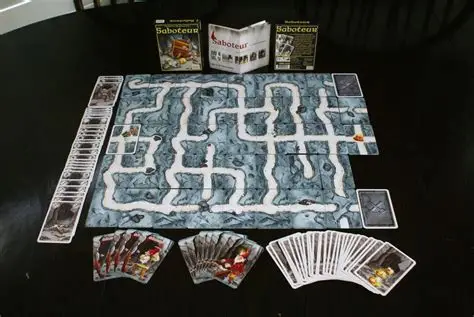
\includegraphics[width=0.75\linewidth]{5.Thiết kế//images/image.png}
    \caption{Bộ bài Saboteur đầy đủ}
    \label{fig:placeholder}
\end{figure}

Luật chơi của Saboteur \cite{saboteur2024} cụ thể như sau:

\begin{enumerate}
\item \textbf{Tổng quan và mục tiêu}

\begin{itemize}
  \item Số người chơi: 3--10.
  \item Mục tiêu:
  \begin{itemize}
      \item \textbf{Gold-Diggers}: mở đường từ Start đến Goal chứa vàng.
      \item \textbf{Saboteurs}: phá để Gold-Diggers không thể đến được vàng.
  \end{itemize}
\end{itemize}

\item \textbf{Trang bị trong bộ Saboteur}

\begin{itemize}
  \item 40 Thẻ đường (path cards): gồm 31 thẻ thông, 9 thẻ cụt
  \item 27 Thẻ hành động (action cards)
  \item 11 Thẻ vai trò (role cards)
\end{itemize}


\item \textbf{Bố trí bàn chơi (Setup)}

\begin{figure}[H]
    \centering
    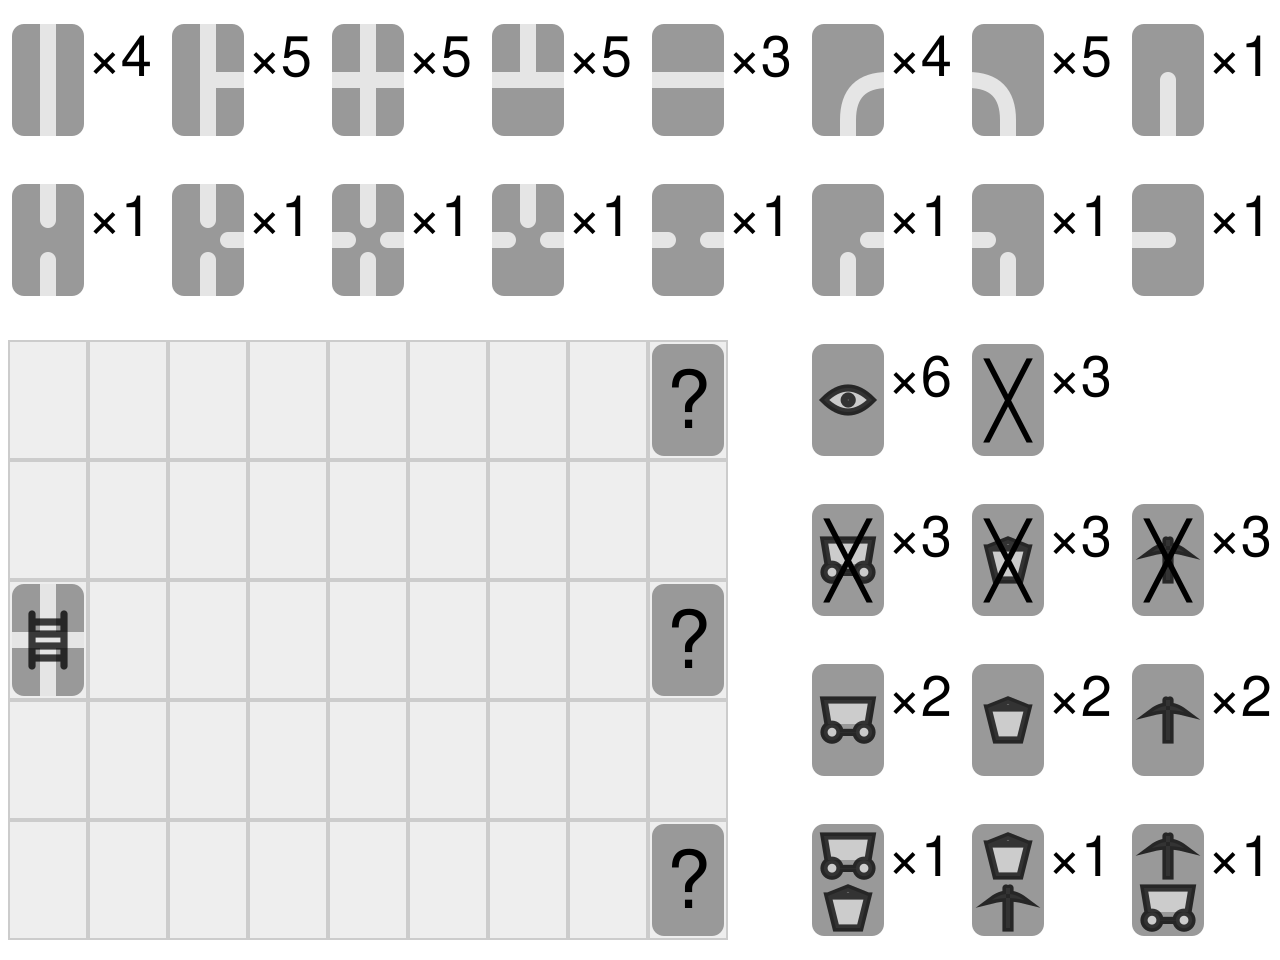
\includegraphics[width=0.75\linewidth]{5.Thiết kế//images/saboteurCards.png}
    \caption{Hình minh họa bộ thẻ và bàn chơi}
    \label{fig:cards-and-board}
\end{figure}


\begin{itemize}
  \item Đặt thẻ Start ở giữa bên trái.
  \item Đặt 3 thẻ Goal úp cách Start 7 khoảng thẻ: 1 giữa, 1 trên, 1 dưới.
  \item Vai trò và số thẻ phát cho mỗi người\\
  % \textbf{Số lượng vai trò theo số người chơi:}
    \begin{table}[h]
    \centering
        \begin{tabular}{|c|c|c|c|c|c|c|c|c|}
        \hline
        Tổng số Người chơi & 3 & 4 & 5 & 6 & 7 & 8 & 9 & 10 \\ \hline
        Số Saboteurs     & 1 & 1 & 2 & 2 & 3 & 3 & 3 & 4 \\ \hline
        Số Gold-Diggers  & 2 & 3 & 3 & 4 & 3 & 4 & 5 & 6 \\ \hline
        \end{tabular}
        \caption{Bảng số lượng vai trò theo số người chơi:}
        \label{tab:total-roles}
    \end{table}
    % \textbf{Số thẻ phát cho mỗi người:}
    \begin{table}[h]
    \centering
        \begin{tabular}{|c|c|c|c|c|c|c|c|c|}
        \hline
        Tổng số Người chơi      & 3 & 4 & 5 & 6 & 7 & 8 & 9 & 10 \\ \hline
        Thẻ mỗi người      & 6 & 6 & 6 & 5 & 5 & 4 & 4 & 4 \\ \hline
        \end{tabular}
        \caption{Bảng số thẻ phát cho mỗi người}
        \label{tab:cards-per-player}
    \end{table}

    \item Tất cả những lá bài còn lại được xáo lại thành chồng và để úp xuống bàn.
\end{itemize}


\item \textbf{Luật chơi}

\begin{itemize}
  \item Lượt xoay chiều kim đồng hồ.
  \item Mỗi lượt chọn một trong các hành động:
  \begin{enumerate}
    \item Đặt thẻ đường (path card).
    \item Chơi thẻ hành động (action card).
    \item Bỏ thẻ (discard).
  \end{enumerate}
  \item Sau khi xong lượt của mình, người chơi bốc lên thẻ trên cùng của deck, lượt chơi tiếp tục qua người tiếp theo.
  \item Gold-Diggers thắng khi có đường nối (phải là đường thông) từ start tới goal chứa vàng. Saboteurs thắng khi tất cả đã hết bài mà vẫn chưa nối được đường tới vàng.
\end{itemize}

% ========================================================
% 6. PATH CARDS
% ========================================================
\item \textbf{Thẻ đường (Path Cards)}
\begin{figure}[H]
    \centering
    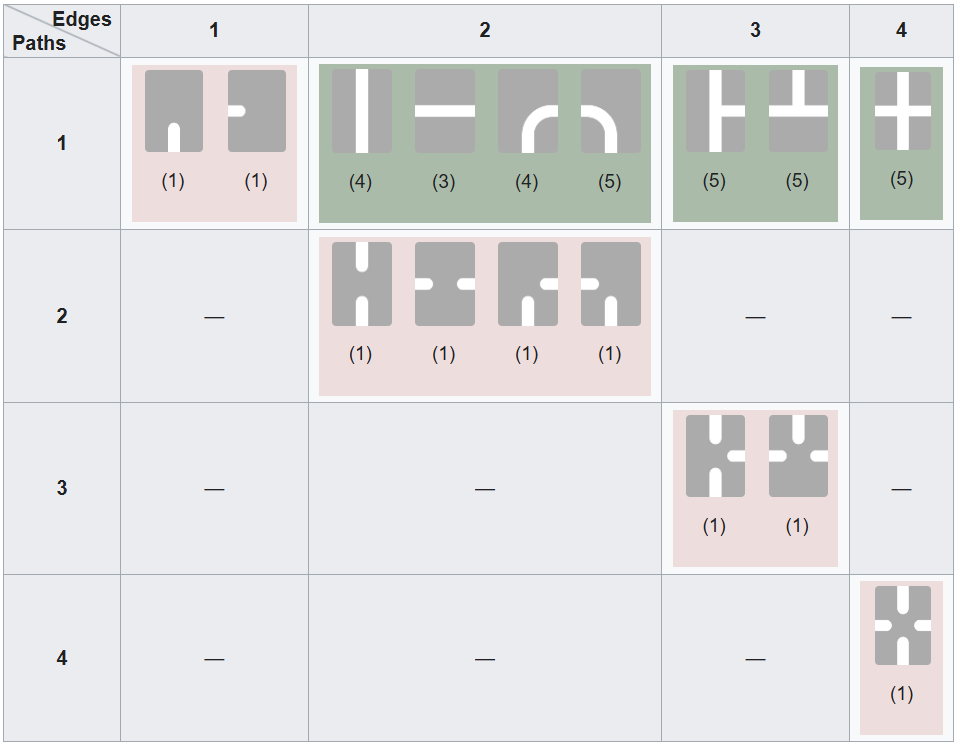
\includegraphics[width=0.75\linewidth]{5.Thiết kế//images/pathCards.png}
    \caption{Phân loại thẻ đường}
    \label{fig:placeholder}
\end{figure}
% \fbox{\parbox[c][4cm][c]{0.85\textwidth}{\centering (Placeholder) Các loại path cards}}
\begin{itemize}
  \item \textbf{Phân loại thẻ Đường}  
  Thẻ Đường (\emph{Path cards}) trong Saboteur được dùng để tạo ra mạng lưới đường hầm từ vị trí xuất phát đến các thẻ mục tiêu. Chúng được chia thành:
  \begin{itemize}
    \item \textbf{Thẻ đường thẳng}: nối liền hai đầu theo trục ngang hoặc dọc.
    \item \textbf{Thẻ giao nhau}: có nhiều nhánh rẽ, cho phép mở rộng đường theo nhiều hướng.
    \item \textbf{Thẻ cụt (dead-end)}: Có thể nối với các thể khác nhưng không được tính là thông đường.
    \item \textbf Các cạnh thẻ không có lối được tính là tường,  khiến người chơi không thể nối đường theo hướng đó.
  \end{itemize}

  \item \textbf{Cách đặt thẻ Đường hợp lệ}  
  Một thẻ Đường được xem là hợp lệ khi thỏa các điều kiện sau:
  \begin{itemize}
    \item Các đầu đường (lối ra) trên thẻ mới phải khớp với đầu đường của thẻ đã có trên bàn: đường nối với đường, tường nối với tường.
    \item Không được tạo ra một kết nối trái ngược (ví dụ: đầu đường mở nối vào tường bịt).
    \item Thẻ phải được đặt kề cạnh một thẻ đã có sẵn trong mạng lưới (không được “nhảy cóc”).
    % \item Người chơi không được phá vòng lặp đang tồn tại trừ khi dùng thẻ hành động chuyên biệt.
  \end{itemize}

  \item \textbf{Quy tắc xoay thẻ}  
  Tất cả thẻ Đường đều có thể được xoay 180° trước khi đặt xuống.  
  \begin{itemize}
    \item Người chơi không được xoay 90°; chỉ xoay 180° vì cấu trúc hầm được thiết kế theo hai hướng chính.
    \item Sau khi xoay, thẻ vẫn phải thỏa điều kiện kết nối hợp lệ như đã nêu ở mục trên.
  \end{itemize}

  \item \textbf{Phá đường bằng thẻ Bomb}  
  Thẻ \emph{Bomb} là thẻ hành động dùng để phá hủy một thẻ Đường đã được đặt trên bàn.
  \begin{itemize}
    \item Người chơi chọn một thẻ Đường bất kỳ (trừ thẻ Start và thẻ Goal) để loại bỏ.
    \item Sau khi phá, ô trống được để lại và không có thẻ nào tự động dịch chuyển vào.
    \item Bomb không được dùng để phá thẻ trên tay người chơi, chỉ phá thẻ đã đặt.
  \end{itemize}

\end{itemize}
% ========================================================
% 7. ACTION CARDS
% ========================================================
\item \textbf{Thẻ hành động (Action Cards)} 

Các thẻ hành động ảnh hưởng trực tiếp đến khả năng đặt thẻ đường hoặc quan sát thông tin trong ván chơi.  
Trong game có \textbf{3 loại công cụ}: 
\begin{itemize}
    \item Xe đẩy (\textit{Cart})
    \item Xẻng (\textit{Shovel})
    \item Mũ (\textit{Hat})
\end{itemize}

Nếu người chơi bị phá \textbf{bất kỳ một trong ba công cụ}, họ \textbf{không thể đặt thẻ đường}.  
Để sửa, người chơi phải dùng thẻ Repair tương ứng.

\begin{itemize}
    \item \textbf{Repair đơn}: sửa đúng 1 công cụ được chỉ định trên thẻ.
    \item \textbf{Repair kép}: sửa 1 trong 2 công cụ hiển thị trên thẻ (Có biến thể có thể sửa cả hai đồng thời).
\end{itemize}

\begin{table}[H]
\centering
\begin{tabular}{|c|p{7cm}|c|}
\hline
\textbf{Loại thẻ} & \textbf{Công dụng} & \textbf{Số lượng} \\ \hline
Sabotage & Phá 1 công cụ: Cart, Shovel hoặc Hat. Người bị phá không thể đặt Path cho đến khi được sửa. & 9 \\ \hline
Repair   & Sửa công cụ bị phá. Gồm: 6 thẻ đơn (mỗi loại công cụ 2 thẻ), 3 thẻ kép. & 9 \\ \hline
Map      & Cho phép xem lén 1 trong 3 thẻ Goal. Không được tiết lộ thông tin trừ khi tự nguyện. & 6 \\ \hline
Rockfall & Phá hủy 1 Path card trên bàn (trừ Start và 3 Goal). Thẻ bị phá được loại khỏi mỏ. & 3 \\ \hline
\end{tabular}
\end{table}

% \end{itemize}

\end{enumerate}
\subsection{Sáng tạo luật chơi mới - Biến thể Saboteur với  ngày đêm }
Biến thể mới giữ nguyên tinh thần bluffing và phản bội của Saboteur gốc nhưng bổ sung cơ chế pha \textbf{ngày} - \textbf{đêm}, thời gian giới hạn, tranh luận, bỏ phiếu và một số thẻ hành động mới mạnh mẽ hơn. Trò chơi vẫn chia hai phe: \textbf{Thiện (Gold-Diggers - Chó)} và \textbf{Ác (Saboteurs - Mèo)}, sử dụng bộ bài gồm thẻ đường (path cards) và thẻ hành động (action cards). Mục tiêu thắng thua giữ nguyên như phiên bản gốc.
\begin{enumerate}
\item \textbf{Chuẩn bị trước khi bắt đầu game}
\begin{itemize}
\item Chia vai trò (role cards) theo bảng phân bổ của phiên bản gốc (xem bảng \ref{tab:total-roles} - số lượng Saboteurs và Gold-Diggers theo tổng số người chơi).
\item \textbf{Thêm số lượng thẻ đường}: Sử dụng toàn bộ thẻ đường của bộ gốc, nhưng \textbf{ngẫu nhiên loại bỏ 10 thẻ đường} trước khi xào bài và để không ai biết chính xác số lượng cũng như loại thẻ đường nào còn lại trong bộ bài.
\item Chia bài cho mỗi người chơi như cũ theo bảng \ref{tab:cards-per-player} 
\item Xào phần bài còn lại thành chồng bài úp (draw pile).
\item Bố trí bàn chơi giống phiên bản gốc (xem hình \ref{fig:cards-and-board}).
\end{itemize}
\item \textbf{Cấu trúc một round}
\\
Mỗi round được chia thành hai pha chính: \textbf{Đêm} và \textbf{Ngày}.
\\
\textbf{Đêm (Night Phase):}
\begin{itemize}
\item Màn hình/bản đồ tối lại, người chơi \textbf{không nhìn thấy bất kỳ thay đổi nào trên bản đồ} ngoại trừ thông tin lượt hiện tại.
\item Thứ tự lượt chơi trong đêm được \textbf{xếp ngẫu nhiên} (không theo chiều kim đồng hồ như bản gốc).
\item Mỗi người chơi lần lượt thực hiện lượt:
\begin{itemize}
\item Bản đồ tạm thời hiện ra cho riêng người đó.
\item Trong \textbf{15--30 giây} (có thể tùy chỉnh), người chơi thực hiện một trong các hành động quen thuộc:
\begin{enumerate}
\item Đặt thẻ đường (path card) – phải tuân thủ đầy đủ quy tắc kết nối và xoay thẻ như bản gốc.
\item Chơi thẻ hành động (action card).
\item Bỏ bài (discard).
\end{enumerate}
\item Sau khi hết thời gian hoặc xác nhận hành động, bản đồ lại tối đi với người chơi đó.
\item Bốc 1 lá bài từ chồng bài úp (nếu còn).
\end{itemize}
\item Khi tất cả người chơi đã hoàn thành lượt trong đêm, pha Đêm kết thúc và chuyển sang pha Ngày.
\end{itemize}



\textbf{Ngày (Day Phase):}
\begin{itemize}
\item Bản đồ được chiếu sáng hoàn toàn, mọi người chơi cùng nhìn thấy toàn bộ thay đổi đã xảy ra trong pha Đêm.
\item Người chơi có \textbf{60 giây} (có thể tùy chỉnh) để \textbf{trò chuyện, tranh luận, biện minh} và đọc vị nhau.
\item Cuối pha Ngày, thực hiện \textbf{bỏ phiếu}:
\begin{itemize}
\item Có thể vote \textbf{skip} (không loại ai) hoặc vote một người chơi cụ thể.
\item Người bị vote nhiều phiếu nhất sẽ bị \textbf{cấm chơi 1 round tiếp theo} (không được hành động trong pha Đêm của round sau).
\end{itemize}
\end{itemize}

\item \textbf{Kết thúc game}
Giữ nguyên luật thắng thua của phiên bản gốc:
\begin{itemize}
\item Phe Thiện (Chó) thắng nếu có đường thông hợp lệ từ thẻ Start đến thẻ Goal chứa vàng.
\item Phe Ác (Mèo) thắng nếu hết bài trên tay tất cả người chơi mà vẫn chưa nối được đường đến vàng.
\end{itemize}
\item \textbf{Thẻ hành động mới (bổ sung thêm vào bộ bài)}
\begin{table}[H]
\centering
\begin{tabular}{|l|p{7cm}|p{5cm}|}
\hline
\textbf{Tên thẻ} & \textbf{Công dụng} & \textbf{Ghi chú} \\ \hline
Shield & Người chơi sẽ có khiên vĩnh viễn có thể đỡ được 1 đòn tấn công phá công cụ (Cart, Shovel, Hat) bởi thẻ Sabotage. & Có thể áp dụng cho bất cứ ai, không tích lũy \\ \hline
Binoculars & Khi sử dụng thẻ này, người chơi được nhìn thấy toàn bộ bản đồ từ lúc chơi thẻ cho đến hết Đêm hiện tại. & Có thể áp dụng cho bất cứ ai\\ \hline
Swap Goals & Trong Đêm, tráo vị trí ngẫu nhiên hoặc chỉ định của 3 thẻ Goal (khi chúng vẫn đang úp). & Thay đổi vị trí kho vàng thực sự \\ \hline
\end{tabular}
\caption{Các thẻ hành động mới}
\end{table}
\end{enumerate}


\subsection{Mục tiêu của đề tài}
    Từ những phân tích về thực trạng và nhu cầu thị trường nêu trên, nhóm thực hiện đề tài xác định các mục tiêu cốt lõi cần đạt được như sau:\\

    \textbf{Thứ nhất, số hóa và tự động hóa trọn vẹn luật chơi Saboteur:}
    Mục tiêu đầu tiên là xây dựng một hệ thống logic game hoàn chỉnh, đảm bảo tuân thủ chính xác luật chơi gốc của board game Saboteur. Hệ thống phải tự động xử lý các thao tác phức tạp như chia bài, kiểm tra vai trò (Role), thuật toán loang để xác định đường đi liên thông từ điểm xuất phát đến kho báu, và tính toán thắng thua. Điều này nhằm loại bỏ sự rườm rà trong việc thiết lập bàn chơi (setup) thủ công, giúp người chơi tập trung hoàn toàn vào chiến thuật.\\
    
    \textbf{Thứ hai, xây dựng thêm phiên bản Saboteur mở rộng kết hợp cơ chế Ma Sói (Werewolf):} Mục tiêu của đề tài là phát triển thêm một phiên bản Saboteur hoàn toàn mới bằng cách tích hợp các yếu tố đặc trưng của Ma Sói nhằm tăng tính chiến thuật và tương tác giữa người chơi. Cụ thể, trò chơi được thiết kế với hai giai đoạn ngày và đêm, cho phép người chơi thảo luận, suy luận và bỏ phiếu trong pha ngày để xác định người bị nghi ngờ; người có số phiếu cao nhất sẽ bị cấm lượt đi trong đêm tiếp theo. Sự kết hợp giữa cơ chế xây dựng đường đi của Saboteur và yếu tố ẩn vai trò, đấu trí của Ma Sói giúp tạo ra trải nghiệm chơi mới mẻ, kịch tính và giàu tính chiến thuật hơn so với các phiên bản hiện có.\\
    
    \textbf{Thứ ba, xây dựng môi trường tương tác xã hội 3D:}
    Khác với các ứng dụng chơi bài 2D truyền thống, mục tiêu của nhóm là tạo ra một không gian 3D sống động – nơi người chơi không chỉ là những cái tên trên bảng điểm. Người chơi sẽ được hóa thân vào các nhân vật (Avatar), có khả năng di chuyển tự do trong không gian sảnh chờ (Lobby) và bàn chơi. Mục tiêu là tái hiện cảm giác "tụ tập" thực tế, nơi các tương tác vật lý và phi ngôn ngữ được đề cao.\\
    
    \textbf{Thứ tư, phát triển các tính năng giải trí bổ trợ:}
    Để giải quyết bài toán "thời gian chết" (downtime) khi chờ đợi người khác đánh bài hoặc chờ đủ người tạo phòng, nhóm đặt mục tiêu tích hợp các mini-features mang tính giải trí cao. Cụ thể là hệ thống nhạc cụ ảo (cho phép người chơi tương tác phím để tạo âm thanh) và hệ thống thời trang (thay đổi ngoại hình nhân vật). Đây là yếu tố then chốt để giữ chân người chơi và tạo nên sự vui nhộn đặc trưng của dòng Party Game.\\
    
    \textbf{Thứ năm, hoàn thiện kỹ thuật Multiplayer thời gian thực:}
    Ứng dụng kiến thức về lập trình mạng để xây dựng hệ thống Client-Host ổn định. Đảm bảo sự đồng bộ mượt mà về vị trí nhân vật, trạng thái bàn chơi và các tương tác thời gian thực giữa nhiều người chơi khác nhau, giảm thiểu độ trễ (latency) để trải nghiệm không bị gián đoạn.
    
\subsection{Phạm vi thực hiện}

    Về nền tảng, trò chơi hướng đến việc chơi trò chơi trên nền tảng Window từ phiên bản Window 7 trở lên.
    
    Về đối tượng hướng đến của trò chơi, trò chơi hướng đến tất cả mọi người ở mọi lứa tuổi cần sự giải trí, sự mới mẻ, sự cạnh tranh và tư duy giải đố.


\subsection{Ý nghĩa và tính ứng dụng của đề tài}

    \textbf{Ý nghĩa khoa học và thực tiễn:}
    Việc thực hiện đề tài "Fishy Business" không chỉ là việc tạo ra một sản phẩm giải trí đơn thuần, mà còn là cơ hội để nhóm áp dụng tổng hợp các kiến thức nền tảng của ngành Khoa học máy tính.
    \begin{itemize}
        \item \textit{Thử thách về Lập trình mạng:} Đồng bộ hóa trạng thái trong môi trường 3D là một bài toán khó, đòi hỏi sự hiểu biết sâu sắc về cấu trúc gói tin, băng thông và xử lý độ trễ.
        \item \textit{Tư duy Thiết kế hệ thống (System Design):} Việc kết hợp giữa logic chặt chẽ của một game bài (Turn-based) với sự tự do của một game nhập vai (Real-time 3D) đòi hỏi một kiến trúc phần mềm linh hoạt, dễ bảo trì và mở rộng (Design Patterns).
    \end{itemize}
    
    \textbf{Tính ứng dụng:}
    \begin{itemize}
        \item \textit{Giải trí và Kết nối:} Trong bối cảnh làm việc và học tập từ xa ngày càng phổ biến, sản phẩm đóng vai trò là cầu nối giúp bạn bè, đồng nghiệp có không gian để "gặp gỡ" và giải trí cùng nhau mà không bị giới hạn bởi khoảng cách địa lý.
        \item \textit{Tiềm năng mở rộng:} Dự án được xây dựng với kiến trúc hướng đối tượng (OOP), do đó có thể dễ dàng mở rộng để tích hợp thêm nhiều board game khác nhau (như Ma Sói, Mèo Nổ) vào cùng một game trong tương lai, hướng tới mô hình "Metaverse" thu nhỏ cho board game.
    \end{itemize}

\subsection{So sánh một số game tương tự trên thị trường}
Để định vị sản phẩm rõ ràng hơn, nhóm tiến hành so sánh \textit{Fishy Business} với các sản phẩm cạnh tranh trên nền tảng PC và Web.

\subsubsection{Tabletop Simulator (PC - Steam)}
Đây là "tượng đài" của dòng game mô phỏng board game trên PC.
\begin{itemize}
    \item \textbf{Điểm mạnh:} Mô phỏng vật lý cực kỳ chân thực, kho game khổng lồ từ Workshop.
    \item \textbf{Điểm yếu cần khắc phục:} Tabletop Simulator là một môi trường "Sandbox" thuần túy. Nó không có luật chơi tự động (người chơi phải tự tính điểm, tự xào bài bằng tay ảo). Hơn nữa, nó khá nặng nề và phức tạp cho những người chơi casual (phổ thông). Người chơi không có nhân vật để đi lại tương tác với môi trường, dẫn đến thiếu cảm giác kết nối xã hội.
\end{itemize}

\subsubsection{Board Game Arena (Web-based)}
Nền tảng chơi board game trên trình duyệt web rất phổ biến.
\begin{itemize}
    \item \textbf{Điểm mạnh:} Nhanh, tiện, chạy trên mọi trình duyệt, luật chơi tự động hóa tốt.
    \item \textbf{Điểm yếu cần khắc phục:} Đồ họa 2D hoàn toàn tĩnh. Trải nghiệm chơi giống như đang làm việc với một file Excel có hình ảnh hơn là chơi game. Không có âm nhạc, không có không khí, không có tương tác giữa các người chơi ngoài khung chat text bé tí.
\end{itemize}

\subsubsection{Sự khác biệt của Fishy Business}
\textit{Fishy Business} chọn một lối đi riêng trên PC:
\begin{itemize}
    \item \textbf{Trải nghiệm 3D Native:} Không phải là web game, đây là một ứng dụng Windows Standalone tận dụng sức mạnh đồ họa để tạo ra không gian đẹp mắt.
    \item \textbf{Kết hợp hoàn hảo:} Nhóm lấy sự tiện lợi (luật chơi tự động) của \textit{Board Game Arena} kết hợp với sự tự do, vui nhộn (di chuyển, nghịch ngợm) của các game như \textit{Overcooked} hay \textit{Party Animals}.
    \item \textbf{Tính năng độc nhất:} \textit{Fishy Business} kết hợp cơ chế xây dựng đường đi của Saboteur với yếu tố ẩn vai trò và suy luận theo phong cách Ma Sói trong hai pha ngày – đêm, kèm hệ thống thảo luận và bỏ phiếu. Đặc biệt, cơ chế “cấm lượt đi” tạo ra biến động chiến thuật liên tục, mang lại trải nghiệm mới lạ và kịch tính hơn so với Saboteur truyền thống.
\end{itemize}

\newpage
\section{Yêu cầu của đề tài}
Dựa trên mục tiêu xây dựng một tựa game Multiplayer kết hợp giữa tư duy chiến thuật và tương tác xã hội trên nền tảng PC, nhóm xác định các yêu cầu cụ thể đối với hệ thống như sau. Việc phân định rõ ràng các nhóm yêu cầu này là kim chỉ nam cho quá trình thiết kế và lập trình ở các giai đoạn sau.
\subsection{Yêu cầu chức năng}
Đây là những tính năng cốt lõi mà hệ thống bắt buộc phải thực hiện được để đáp ứng nhu cầu của người chơi. Nhóm chia thành hai phân hệ chính: Gameplay và Social.

\subsubsection{Nhóm chức năng Gameplay (Core Loop - Saboteur)}
Hệ thống phải đảm bảo vận hành chính xác logic của board game Saboteur gốc:
\begin{itemize}
    \item \textbf{Quản lý phiên chơi:}
        \begin{itemize}
            \item Cho phép người chơi Tạo phòng (Host Game) và Tham gia phòng (Join Game/Quick Join) thông qua danh sách phòng.
            \item Hỗ trợ tối thiểu 3 người và tối đa 8 người trong một phiên chơi.
        \end{itemize}
    \item \textbf{Cơ chế chia bài và Phân vai:}
        \begin{itemize}
            \item Hệ thống tự động xáo bài và chia bài ngẫu nhiên cho người chơi theo số lượng quy định.
            \item Phân vai ngẫu nhiên (Thợ mỏ - \textit{Chó} hoặc Kẻ phá hoại - \textit{Mèo}) và đảm bảo bí mật vai trò của từng người chơi (chỉ người chơi đó mới thấy vai trò của mình).
        \end{itemize}
    \item \textbf{Cơ chế Đánh bài:}
        \begin{itemize}
            \item \textit{Thẻ đường hầm (Path Cards):} Người chơi có thể đặt thẻ lên bàn chơi. Hệ thống phải kiểm tra tính hợp lệ (logic khớp nối đường đi) trước khi cho phép đặt.
            \item \textit{Thẻ chức năng (Action Cards):} Hỗ trợ các thẻ phá hủy đường hầm, xem bản đồ kho báu, hoặc khóa/mở khóa hành động của người chơi khác.
        \end{itemize}
    \item \textbf{Cơ chế Chiến thắng:}
        \begin{itemize}
            \item Tự động phát hiện khi đường hầm nối liền từ điểm xuất phát đến kho báu (Phe chó thắng).
            \item Tự động kết thúc ván khi hết bài mà chưa tìm thấy kho báu (Phe mèo thắng).
        \end{itemize}
    \item \textbf{Chức năng của bản mở rộng:}
        \begin{itemize}
            \item Cơ chế day-night gồm các phiên như: day, night, discussion, voting.
            \item Chức năng của 3 lá bài mở rộng.
            \item Chức năng vote player, skip trong voting.
        \end{itemize}
\end{itemize}

\subsubsection{Nhóm chức năng Xã hội và Tương tác (Social \& Interactive)}
Tận dụng lợi thế 3D và nền tảng PC để tăng cường trải nghiệm:
\begin{itemize}
    \item \textbf{Điều khiển nhân vật:} Người chơi điều khiển nhân vật 3D di chuyển tự do trong sảnh chờ bằng cụm phím WASD và điều hướng camera bằng Chuột. Phím \textbf{E} để mở menu emotes, nhấn giữ \textbf{F} để tương tác với các vật thể, \textbf{Enter} để mở hộp thoại chat, nhấn giữ \textbf{V} để voice chat.
    \item \textbf{Hệ thống Nhạc cụ:}
        \begin{itemize}
            \item Cung cấp các nhạc cụ ảo ( Piano, ...) trong môi trường game.
            \item Cho phép người chơi kích hoạt nhạc cụ và sử dụng bàn phím máy tính để chơi các nốt nhạc (Note mapping). Âm thanh phát ra phải được đồng bộ đến tai của tất cả người chơi khác trong phòng.
        \end{itemize}
    \item \textbf{Hệ thống Thời trang:}
        \begin{itemize}
            \item Người chơi có thể truy cập kho đồ để thay đổi trang phục (Skin, Mũ, Phụ kiện) cho nhân vật.
            \item Sự thay đổi ngoại hình phải được cập nhật ngay lập tức cho các người chơi khác cùng thấy.
        \end{itemize}
    \item \textbf{Giao tiếp:} Hỗ trợ kênh Chat văn bản (Global Chat), hệ thống biểu cảm (Emotes/Animations) như vẫy tay, nhảy múa và voice chat.
\end{itemize}
\subsection{Yêu cầu phi chức năng}
Yêu cầu về chất lượng và hiệu suất hoạt động của hệ thống:

\begin{itemize}
    \item \textbf{Hiệu năng:}
        \begin{itemize}
            \item Game phải duy trì tốc độ khung hình ổn định (tối thiểu 60 FPS) trên các cấu hình máy tính tầm trung (có card đồ họa rời phổ thông hoặc onboard đời mới).
            \item Thời gian tải màn chơi không quá 10 giây.
        \end{itemize}
    \item \textbf{Độ trễ mạng:}
        \begin{itemize}
            \item Các thao tác quan trọng như đánh bài, di chuyển nhân vật phải được đồng bộ với độ trễ thấp (dưới 100ms trong điều kiện mạng ổn định) để tránh hiện tượng "teleport" hoặc lệch pha.
            \item Đặc biệt, tính năng đánh đàn yêu cầu độ trễ cực thấp để đảm bảo nhịp điệu bài hát không bị vỡ khi nhiều người cùng chơi (Jamming).
        \end{itemize}
    \item \textbf{Tính tin cậy:}
        \begin{itemize}
            \item Hệ thống phải xử lý được các ngoại lệ: người chơi (trừ host) đột ngột mất kết nối không được làm sập phòng chơi của những người còn lại.
        \end{itemize}
    \item \textbf{Khả năng mở rộng:} Kiến trúc code phải được tổ chức theo hướng Modular (mô-đun hóa) để dễ dàng thêm các loại bài mới, role mới hoặc nhạc cụ mới trong tương lai mà không phá vỡ logic cũ.
\end{itemize}

\subsection{Yêu cầu kỹ thuật}
Các ràng buộc về công nghệ và môi trường phát triển:

\begin{itemize}
    \item \textbf{Nền tảng vận hành:}
        \begin{itemize}
            \item Hệ điều hành: Windows 10 (64-bit) hoặc Windows 11.
            \item Thiết bị ngoại vi: Bắt buộc sử dụng Chuột và Bàn phím.
        \end{itemize}
    \item \textbf{Công cụ phát triển:}
        \begin{itemize}
            \item \textit{Game Engine:} Ổn định, hỗ trợ lập trình 3D, multiplayer và hỗ trợ build PC mạnh mẽ.
            \item \textit{Tools:} Visual Studio Code
        \end{itemize}
    \item \textbf{Giải pháp mạng:}
        \begin{itemize}
            \item Sử dụng kiến trúc Client-Server hoặc Host-Client.
            \item Thư viện mạng: Netcode for GameObjects (NGO) hoặc Photon Fusion (tùy chọn dựa trên độ phức tạp).
        \end{itemize}
    \item \textbf{Tài nguyên đồ họa (Assets):}
        \begin{itemize}
            \item Phong cách nghệ thuật: Low-poly và Cel-shading để phù hợp với không khí vui nhộn và tối ưu hiệu năng.
        \end{itemize}
\end{itemize}

\subsection{Yêu cầu trải nghiệm người dùng}

Đối với một game Party, cảm xúc của người chơi là yếu tố sống còn. Nhóm đặt ra các tiêu chuẩn UX sau:

\begin{itemize}
    \item \textbf{Tính trực qua:}
        \begin{itemize}
            \item Giao diện người dùng (UI) phải rõ ràng. Các lá bài trên tay phải dễ nhìn, dễ đọc thông tin.
            \item Thao tác kéo thả bài hoặc click chọn bài phải mượt mà, có phản hồi bằng âm thanh hoặc hiệu ứng hình ảnh khi tương tác thành công.
        \end{itemize}
    \item \textbf{Bầu không khí:}
        \begin{itemize}
            \item Môi trường 3D phải tạo cảm giác ấm cúng, vui vẻ.
            \item Âm nhạc nền nhẹ nhàng, không lấn át tiếng trò chuyện hoặc tiếng nhạc cụ do người chơi tạo ra.
        \end{itemize}
    \item \textbf{Tính phản hồi:}
        \begin{itemize}
            \item Các thông báo quan trọng (tới lượt chơi, tìm thấy vàng, bị phá bài) phải hiển thị nổi bật giữa màn hình.
            \item UI phản hồi nhanh chóng khi nhận tương tác.
            \item Khi người chơi bấm phím đánh đàn, âm thanh phải phát ra ngay lập tức để tạo cảm giác thỏa mãn.
        \end{itemize}
    \item \textbf{Khả năng tiếp cận:} Game cung cấp hướng dẫn cơ bản hoặc Tooltip, giúp người chưa từng chơi Saboteur cũng có thể nắm bắt nhanh chóng.
\end{itemize}

\newpage
\section{Nghiên cứu tổng quan}
Để xây dựng thành công tựa game "Fishy Business", nhóm đã tiến hành nghiên cứu các cơ sở lý thuyết và công nghệ nền tảng liên quan đến phát triển trò chơi điện tử trực tuyến. Nội dung nghiên cứu bao gồm tổng quan về game multiplayer, quy trình phát triển phần mềm, so sánh các game engine phổ biến và kiến trúc mạng máy tính.


\subsection{Tổng quan về game 3D Multiplayer}
    Trò chơi nhiều người chơi (Multiplayer Game) là một hệ thống thời gian thực phức tạp, nơi nhiều người chơi tương tác với nhau trong cùng một môi trường ảo.\\
    
    \textbf{Đặc điểm cốt lõi:}
    Khác với game Single-player (nơi mọi logic diễn ra cục bộ trên một máy), game Multiplayer đối mặt với thách thức lớn nhất là sự \textbf{đồng bộ hóa trạng thái}. Mọi hành động của người chơi A (di chuyển, đánh bài, đánh đàn) phải được truyền tải chính xác và gần như tức thời đến người chơi B, C, D,...
    \begin{itemize}
        \item \textit{Không gian 3D:} Việc đồng bộ trong không gian 3D phức tạp hơn 2D do phải xử lý dữ liệu biến đổi liên tục của vector vị trí (Position), góc xoay (Rotation) và các trạng thái vật lý (Physics) trên cả 3 trục (x, y, z).
        \item \textit{Vấn đề độ trễ:} Đây là yếu tố sống còn. Trên môi trường Internet, gói tin luôn có độ trễ. Các kỹ thuật như \textit{Client-side Prediction} (Dự đoán phía máy khách) và \textit{Lag Compensation} (Bù trễ) là những chủ đề nghiên cứu bắt buộc để đảm bảo trải nghiệm mượt mà.
    \end{itemize}
    
\subsection{Nghiên cứu và lựa chọn mô hình phát triển phần mềm}
Việc lựa chọn quy trình phát triển phần mềm phù hợp quyết định đến khả năng quản lý rủi ro và tiến độ của dự án. Nhóm đã nghiên cứu một số mô hình phổ biến sau:

    \subsubsection{Mô hình Thác nước (Waterfall)}
    \begin{figure}[H]
        \centering
        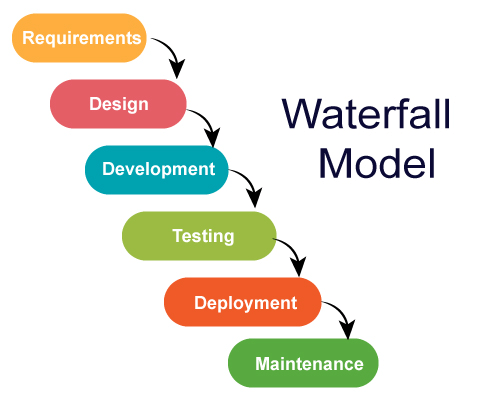
\includegraphics[width=0.7\linewidth]{3.Nghiên cứu/Images/WaterFall.png}
        \caption{Mô hình Waterfall}
        \label{fig:placeholder}
    \end{figure}

    Waterfall model được coi là mô hình phát triển phần mềm đầu tiên được sử dụng. Lý do việc mô hình này được gọi là thác nước vì các giai đoạn phát triển được thực hiện tuần tự và nối tiếp nhau, như một dòng nước chảy. Mỗi giai đoạn hoàn thành trước khi giai đoạn tiếp theo bắt đầu và không có sự quay lại. Do tính chất này, mỗi giai đoạn của mô hình thác nước phải được xác định chính xác.
    
    \subsubsection{Mô hình Agile}
    \begin{figure} [H]
        \centering
        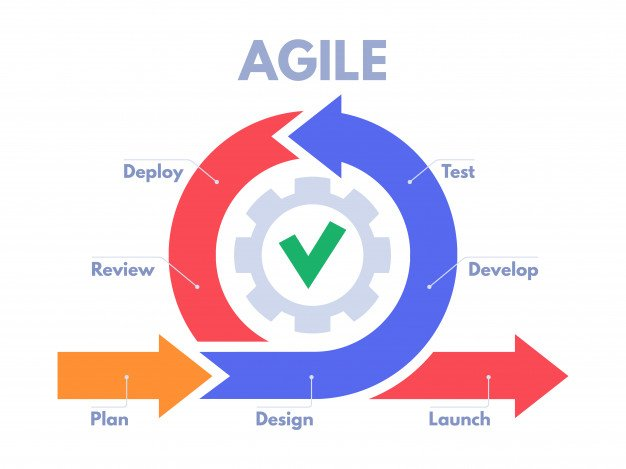
\includegraphics[width=0.7\linewidth]{3.Nghiên cứu//Images/Agile.png}
        \caption{Mô hình Agile}
        \label{fig:placeholder}
    \end{figure}
    Mô hình Agile là một phương pháp phát triển phần mềm linh hoạt. Agile model được tạo ra dựa trên 2 mô hình: Iterative (Lặp lại) và Incremental (Tăng dần). Nó tập trung vào việc phân phối sản phẩm thông qua các chu kỳ phát triển ngắn (gọi là sprint) và thường xuyên nhận phản hồi từ khách hàng. \\
    
    Agile giúp nhóm phát triển dễ dàng thích nghi với các thay đổi yêu cầu, đồng thời cải thiện chất lượng sản phẩm liên tục.
    
    \subsubsection{Quy trình Scrum}
    \begin{figure} [H]
        \centering
        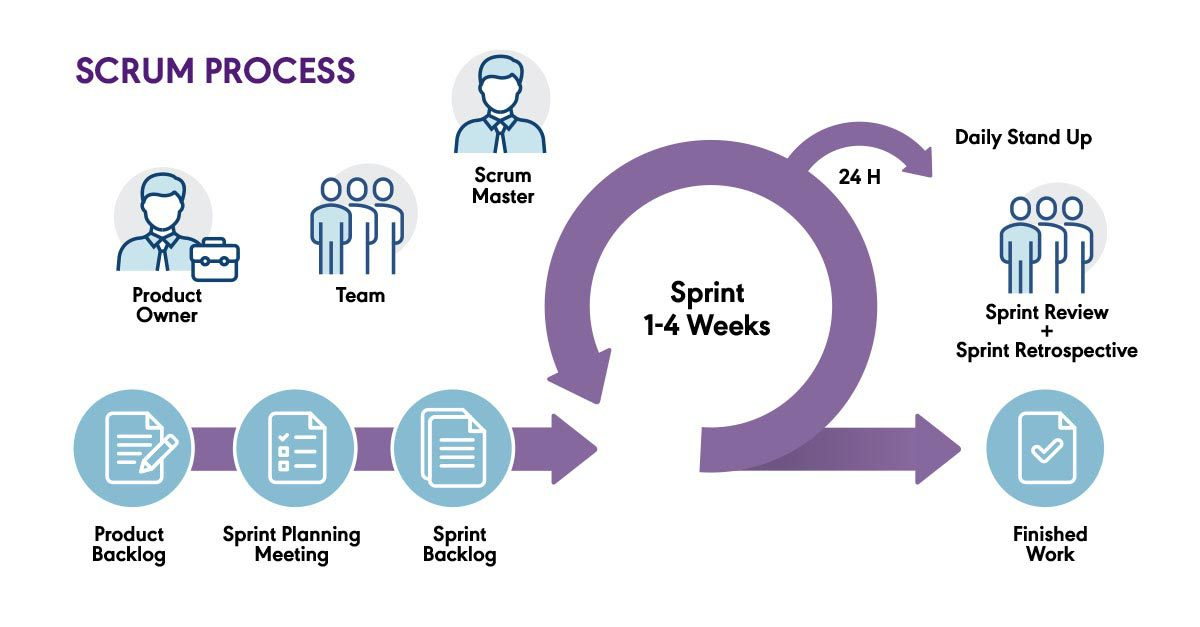
\includegraphics[width=0.75\linewidth]{3.Nghiên cứu//Images/Scrum.png}
        \caption{Scrum Process}
        \label{fig:placeholder}
    \end{figure}
    Scrum là một “khung quản lý dự án” được áp dụng rất rộng rãi từ những dự án đơn giản với một nhóm phát triển nhỏ cho đến những dự án có yêu cầu rất phức tạp với hàng trăm người tham gia. Ngoài ra, Scrum Process cũng phù hợp với những dự án đòi hỏi khung thời gian cố định. \\

    Trong Scrum, công việc sẽ được chia nhỏ thành nhiều giai đoạn gọi là Sprint. Mỗi Sprint chỉ kéo dài từ 1 đến 4 tuần, không quá một tháng. Đầu Sprint sẽ lên kế hoạch làm những yêu cầu nào rồi thực hiện code và test. Cuối Sprint là một sản phẩm hoàn thiện cả code lẫn test có thể demo và chạy được.

    \subsubsection{So sánh các mô hình phát triển dự án phần mềm}
    Mỗi mô hình phát triển dự án đều có các đặc điểm nổi trội riêng, Do đó để phân tích rõ hơn việc lựa chọn giữa các mô hình phát triển để thực hiện dự án, dưới đây là bảng so sánh điểm mạnh và điểm yếu giữa các mô hình:
    \begin{table}[H]
    \centering
    \begin{tabular}{|p{2cm}|p{6cm}|p{6cm}|}
    \hline
    \textbf{Mô hình} & \textbf{Điểm mạnh} & \textbf{Điểm yếu}\\
    \hline
    \textbf{Waterfall} & 
            $\bullet$ Phù hợp với dự án nhỏ và ngắn hạn
            
            $\bullet$ Dễ quản lý, có kế hoạch rõ ràng từ đầu.
            
            $\bullet$ Có sự ổn định cao, ít thay đổi và xác định yêu cầu rõ ràng.
        & 
            $\bullet$ Rất khó để quay lại giai đoạn nào khi nó đã kết thúc
            
            $\bullet$ Ít tính linh hoạt và phạm vi điều chỉnh của nó khá là khó khăn, tốn kém.
         \\
    \hline
    \textbf{Agile} & 
            $\bullet$ Tăng cường khả năng làm việc nhóm.
            
            $\bullet$ Các chức năng được rõ ràng và dễ quản lý.
            
            $\bullet$ Có tính linh hoạt cao.
        & 
            $\bullet$ Không phù hợp với các dự án phức tạp.
            
            $\bullet$ Phụ thuộc vào yếu tố bên ngoài
            
            $\bullet$ Khó kiểm soát tiến độ và deadline.
            
            $\bullet$ Dễ mất định hướng nếu không có kế hoạch rõ ràng.
         \\
    \hline
    \textbf{Scrum} & 
            $\bullet$ Quản lý tiến độ chặt chẽ theo Sprint.
            
            $\bullet$ Theo dõi hiệu suất làm việc rõ ràng.
            
            $\bullet$ Phân chia công việc cụ thể, rõ trách nhiệm.
        & 
            $\bullet$ Nhiều họp, tốn thời gian quy trình.
            
            $\bullet$ Không linh hoạt như Agile thuần.
            
            $\bullet$ Hạn chế việc thay đổi đột ngột giữa Sprint.
         \\
    \hline
    \end{tabular}
    \caption{Bảng So sánh các mô hình phát triển dự án phần mềm}
\end{table}
    Qua bảng phân tích trên, nhóm nhận thấy các đặc điểm của mô hình Scrum là phù hợp với dự án của nhóm nhất. Do đó nhóm quyết định sử dụng mô hình Scrum để phát triển dự án.



\subsection{Nghiên cứu và lựa chọn các công cụ hỗ trợ quản lý dự án}
Trong quy trình Scrum, việc quản lý mã nguồn và tiến độ là bắt buộc. Do đó nhóm đã chọn các công cụ phổ biến sau.
\subsubsection{Discord}
    \begin{figure} [H]
        \centering
        
\includegraphics[width=0.4\linewidth]{3.Nghiên cứu//Images/Discord.png}
        % \caption{Discord}
        \label{fig:placeholder}
    \end{figure}
    Discord là một nền tảng giao tiếp trực tuyến được sử dụng rộng rãi trong lĩnh vực công nghệ thông tin nói chung và lập trình game nói riêng. Trong quá trình thực hiện dự án, Discord đóng vai trò là công cụ hỗ trợ chính cho việc quản lý nhóm, trao đổi kỹ thuật và phối hợp công việc giữa các thành viên. Nhóm sử dụng Discord để tổ chức các buổi họp trực tuyến, thảo luận về hướng phát triển game cũng như xử lý các vấn đề phát sinh trong quá trình làm.\\
    
    Discord cho phép tạo nhiều kênh thảo luận khác nhau theo từng mục đích cụ thể như trao đổi chung, lập trình, thiết kế gameplay và báo lỗi. Việc phân chia kênh giúp nội dung trao đổi được sắp xếp khoa học, tránh chồng chéo thông tin và nâng cao hiệu quả làm việc nhóm. Bên cạnh đó, Discord còn hỗ trợ chia sẻ nhanh các tài nguyên như mã nguồn, hình ảnh, video minh họa gameplay và các tài liệu thiết kế.\\

    Ngoài ra, nền tảng này còn hỗ trợ lưu trữ lịch sử trò chuyện, giúp các thành viên dễ dàng theo dõi lại quá trình thảo luận và quyết định kỹ thuật đã được thống nhất trước đó. Nhờ các tính năng trên, Discord góp phần nâng cao khả năng phối hợp, giảm thời gian trao đổi và hỗ trợ hiệu quả cho việc quản lý và phát triển dự án theo mô hình Scrum.

\subsubsection{Git}
\begin{figure} [H]
    \centering
    
\includegraphics[width=0.4\linewidth]{3.Nghiên cứu//Images/Git.png}
    % \caption{Git}
    \label{fig:placeholder}
\end{figure}
    Git là một hệ thống quản lý phiên bản phân tán mã nguồn mở, được Linus Torvalds phát triển vào năm 2005 nhằm đáp ứng nhu cầu quản lý mã nguồn hiệu quả trong quá trình phát triển nhân hệ điều hành Linux. Cho đến nay, Git đã trở thành một trong những hệ thống quản lý phiên bản phổ biến và được sử dụng rộng rãi nhất trong lĩnh vực phát triển phần mềm. Git cho phép theo dõi toàn bộ lịch sử thay đổi của mã nguồn và hỗ trợ nhiều người làm việc đồng thời trên cùng một dự án.\\

    Một trong những ưu điểm nổi bật của Git là tốc độ xử lý nhanh, khả năng hoạt động ổn định ngay cả với các dự án có quy mô lớn. Git có giao diện dòng lệnh đơn giản, giúp các thành viên trong nhóm dễ dàng tiếp cận và sử dụng. Với đặc tính phân tán hoàn toàn, mỗi thành viên đều sở hữu một bản sao đầy đủ của mã nguồn trên máy cục bộ, cho phép làm việc ngoại tuyến và đồng bộ dữ liệu linh hoạt với các thành viên khác trong nhóm.\\

    Ngoài ra, Git hỗ trợ mạnh mẽ cho việc phát triển song song thông qua cơ chế nhánh (branch), giúp nhiều người có thể phát triển các chức năng khác nhau cùng lúc mà không ảnh hưởng trực tiếp đến mã nguồn chính. Git còn sử dụng các hàm băm mật mã để đảm bảo tính toàn vẹn của dữ liệu, giúp phát hiện nhanh chóng các thay đổi không hợp lệ hoặc sai sót trong quá trình chỉnh sửa mã nguồn. Nhờ những ưu điểm trên, Git đóng vai trò quan trọng trong việc quản lý mã nguồn hiệu quả cho dự án của nhóm.

\subsubsection{Github}
\begin{figure} [H]
    \centering
    
\includegraphics[width=0.4\linewidth]{3.Nghiên cứu//Images/Github.png}
    % \caption{Github}
    \label{fig:placeholder}
\end{figure}
GitHub là một nền tảng lưu trữ và quản lý mã nguồn trực tuyến dựa trên hệ thống quản lý phiên bản Git, được sử dụng rộng rãi trong cộng đồng phát triển phần mềm. Trong quá trình thực hiện dự án, GitHub được nhóm sử dụng để lưu trữ mã nguồn, đồng bộ dữ liệu giữa các thành viên và quản lý tiến độ phát triển dự án.\\

GitHub hỗ trợ làm việc nhóm thông qua các chức năng như kho lưu trữ (repository), nhánh (branch), gộp mã (merge) và yêu cầu hợp nhất (pull request). Nhờ đó, các thành viên có thể phát triển song song các chức năng khác nhau mà không gây ảnh hưởng trực tiếp đến mã nguồn chính. Ngoài ra, GitHub còn cung cấp hệ thống theo dõi lỗi (Issues), giúp ghi lại các lỗi phát sinh và phân công nhiệm vụ cho từng thành viên một cách rõ ràng.\\

Bên cạnh đó, GitHub còn lưu trữ đầy đủ lịch sử thay đổi của mã nguồn, giúp dễ dàng kiểm tra, khôi phục các phiên bản trước khi cần thiết. Nhờ những tính năng trên, GitHub đóng vai trò quan trọng trong việc quản lý mã nguồn, hỗ trợ làm việc nhóm hiệu quả và đảm bảo tính an toàn cho dự án của nhóm.

\subsubsection{Jira}
\begin{figure} [H]
    \centering
    
\includegraphics[width=0.4\linewidth]{3.Nghiên cứu//Images/Jira.png}
    % \caption{Jira}
    \label{fig:placeholder}
\end{figure}
Jira là một công cụ quản lý dự án và theo dõi tiến độ công việc do công ty Atlassian phát triển, được sử dụng phổ biến trong các dự án phát triển phần mềm theo mô hình Agile và Scrum. Trong quá trình thực hiện dự án của nhóm, Jira được nhóm sử dụng để quản lý công việc, theo dõi tiến độ từng giai đoạn và kiểm soát hiệu quả làm việc của các thành viên.\\

Jira cho phép tạo và quản lý các đầu việc (Issue) như Task, Bug, Story, từ đó phân công nhiệm vụ cụ thể cho từng thành viên trong nhóm. Mỗi công việc đều có trạng thái rõ ràng như ``To Do'', ``In Progress'', ``Done'', giúp nhóm dễ dàng theo dõi tiến độ thực hiện. Bên cạnh đó, Jira còn hỗ trợ xây dựng bảng Scrum, lập kế hoạch Sprint và theo dõi khối lượng công việc trong từng Sprint một cách trực quan.\\

Ngoài ra, Jira còn cung cấp các công cụ thống kê và báo cáo tiến độ như biểu đồ Burndown Chart, Velocity Chart, giúp nhóm đánh giá hiệu suất làm việc theo từng giai đoạn. Nhờ những tính năng trên, Jira hỗ trợ hiệu quả cho việc quản lý tiến độ, phân công nhiệm vụ và kiểm soát chất lượng dự án theo mô hình Scrum.



\subsection{Nghiên cứu so sánh và lựa chọn Game Engine}
Game engine là một phần mềm chuyên dụng được sử dụng để thiết kế và phát triển trò chơi điện tử. Có thể hiểu đơn giản, game engine đóng vai trò là một phần mềm trung gian, kết nối và quản lý sự tương tác giữa nhiều thành phần trong cùng một hệ thống trò chơi. Các chức năng cốt lõi của game engine chủ yếu liên quan đến việc làm việc trực tiếp với phần cứng, bao gồm: công cụ dựng hình đồ họa hai chiều và ba chiều, hệ thống vật lý dùng để phát hiện và xử lý va chạm, xử lý âm thanh, quản lý hình ảnh động.\\

Ngoài các chức năng cơ bản, nhiều game engine hiện nay còn tích hợp các gói mở rộng nhằm hỗ trợ những tính năng nâng cao như kết nối mạng, xử lý luồng dữ liệu, tối ưu hóa quá trình kết xuất hình ảnh và hiệu năng của trò chơi. Nhờ có game engine, quá trình phát triển trò chơi điện tử được rút ngắn đáng kể, giúp lập trình viên tiết kiệm thời gian và công sức thông qua việc tái sử dụng và mở rộng các thành phần có sẵn để tạo ra nhiều sản phẩm game khác nhau.\\

Hiện nay, trên thị trường có rất nhiều game engine với những ưu điểm và hạn chế riêng, phù hợp với từng thể loại trò chơi và mục đích phát triển khác nhau. Một số game engine phổ biến sẽ được trình bày ở các mục tiếp theo.

\subsubsection{Unity}

\begin{figure} [H]
    \centering
    
\includegraphics[width=0.4\linewidth]{3.Nghiên cứu//Images/Unity.png}
    % \caption{Unity}
    \label{fig:placeholder}
\end{figure}
Unity là một game engine được phát hành lần đầu vào năm 2005 và nhanh chóng trở thành một trong những nền tảng phát triển trò chơi phổ biến nhất hiện nay. Unity được nhiều nhà phát triển lựa chọn nhờ tính linh hoạt, dễ sử dụng và khả năng hỗ trợ xây dựng trò chơi đa nền tảng như Windows, Linux, macOS, thiết bị di động (Android, iOS) và trình duyệt web. Game engine này đặc biệt phổ biến trong lĩnh vực phát triển game di động và các trò chơi độc lập (indie).\\

Unity hỗ trợ phát triển cả trò chơi hai chiều (2D) và ba chiều (3D), cho phép mô phỏng các tương tác và hiệu ứng trong môi trường ảo một cách trực quan. Ngôn ngữ lập trình chính được sử dụng trong Unity là C\#, giúp lập trình viên dễ dàng tiếp cận và phát triển các chức năng cho trò chơi. Bên cạnh đó, Unity còn hỗ trợ các pipeline kết xuất hình ảnh hiện đại như HDRP (High Definition Render Pipeline) và URP (Universal Render Pipeline), giúp nâng cao chất lượng đồ họa và tối ưu hiệu năng.\\

Ngoài các công cụ phát triển cốt lõi, Unity còn cung cấp kho tài nguyên phong phú thông qua Unity Asset Store, bao gồm mô hình 3D, âm thanh, plugin và các công cụ hỗ trợ phát triển game. Đồng thời, Unity sở hữu một cộng đồng phát triển lớn và năng động, sẵn sàng hỗ trợ và giải đáp các thắc mắc cho người mới. Nhờ những ưu điểm trên, Unity là một lựa chọn phù hợp cho việc phát triển đồ án lập trình game của nhóm.


\subsubsection{Unreal Engine}

\begin{figure} [H]
    \centering
    
\includegraphics[width=0.3\linewidth]{3.Nghiên cứu//Images/Unreal.png}
    % \caption{Unreal Engine}
    \label{fig:placeholder}
\end{figure}
Unreal Engine là một game engine mạnh mẽ do Epic Games phát triển, được phát hành lần đầu vào năm 1998 và hiện nay đã trở thành một trong những công cụ phổ biến nhất trong lĩnh vực phát triển game 3D. Unreal Engine được sử dụng rộng rãi để phát triển các trò chơi có đồ họa chất lượng cao trên nhiều nền tảng như Windows, macOS, Linux, console và thiết bị di động.\\

Unreal Engine hỗ trợ lập trình bằng ngôn ngữ C++ và hệ thống lập trình trực quan Blueprint, giúp cả lập trình viên chuyên nghiệp lẫn người mới đều có thể tiếp cận và phát triển trò chơi. Engine này nổi bật với khả năng kết xuất hình ảnh chân thực, hệ thống ánh sáng tiên tiến, vật lý mạnh mẽ và các công cụ hỗ trợ trí tuệ nhân tạo cho nhân vật trong game.\\

Ngoài ra, Unreal Engine còn cung cấp nhiều công cụ hỗ trợ phát triển như hệ thống vật lý, âm thanh, mạng và tối ưu hiệu năng. Cùng với cộng đồng người dùng lớn và kho tài nguyên phong phú, Unreal Engine là lựa chọn phù hợp cho các dự án game quy mô lớn và các trò chơi đòi hỏi chất lượng đồ họa cao.


\subsubsection{Godot}

\begin{figure} [H]
    \centering
    
\includegraphics[width=0.4\linewidth]{Godot.png}
    % \caption{Godot Engine}
    \label{fig:placeholder}
\end{figure}
Godot là một game engine mã nguồn mở được phát triển nhằm phục vụ cho việc xây dựng các trò chơi 2D và 3D. Godot nổi bật với ưu điểm miễn phí hoàn toàn, không yêu cầu trả phí bản quyền và cho phép người dùng toàn quyền chỉnh sửa mã nguồn theo nhu cầu. Nhờ đó, Godot được sử dụng rộng rãi trong cộng đồng lập trình game độc lập (indie) và giáo dục.\\

Godot hỗ trợ đa nền tảng như Windows, Linux, macOS, Android, iOS và trình duyệt web. Engine này sử dụng các ngôn ngữ lập trình như GDScript (ngôn ngữ riêng của Godot có cú pháp tương tự Python), C\#, và C++. Hệ thống scene và node của Godot giúp việc tổ chức đối tượng trong game trở nên rõ ràng, linh hoạt và dễ quản lý.\\

Ngoài ra, Godot còn tích hợp sẵn các hệ thống vật lý, âm thanh, xử lý va chạm, hoạt ảnh và trí tuệ nhân tạo. Với dung lượng nhẹ, giao diện thân thiện, cộng đồng phát triển ngày càng lớn và tài liệu hướng dẫn phong phú, Godot là một lựa chọn phù hợp cho các dự án game nhỏ, game học tập và đồ án lập trình game.

\subsubsection{So sánh các game engine}
Mỗi phần mềm Game engine đều có các đặc điểm nổi trội riêng, Do đó để phân tích rõ hơn việc lựa chọn giữa các Game engine để thực hiện dự án, dưới đây là bảng so sánh điểm mạnh và điểm yếu giữa các phần mềm Game engine:

\begin{table}[H]
\centering
\begin{tabular}{|p{2cm}|p{4cm}|p{4cm}|p{4cm}|}
\hline
\textbf{Tiêu chí} & \textbf{Unity} & \textbf{Unreal Engine} & \textbf{Godot} \\
\hline
\textbf{Ngôn ngữ} 
& C\#: Dễ học, phổ biến 
& C++ / Blueprint: Mạnh, khó 
& GDScript: Giống Python, dễ \\
\hline
\textbf{Đồ họa} 
& Tốt (URP, HDRP) 
& Rất cao (Nanite, Lumen) 
& Khá, nhẹ \\
\hline
\textbf{2D/3D} 
& Mạnh cả 2D và 3D 
& Mạnh 3D 
& Mạnh 2D, 3D cơ bản \\
\hline
\textbf{Hiệu năng} 
& Tốt, ổn định 
& Rất cao 
& Nhẹ, đủ dùng \\
\hline
\textbf{Cộng đồng} 
& Rất lớn 
& Lớn 
& Đang phát triển \\
\hline
\textbf{Phần cứng} 
& Trung bình 
& Cao 
& Thấp \\
\hline
\textbf{Networking} 
& Mạnh (Netcode, Photon) 
& Tích hợp tốt 
& Cơ bản \\
\hline
\textbf{Chi phí} 
& Miễn phí cơ bản 
& Có phí theo điều kiện 
& Miễn phí 100\% \\
\hline
\textbf{Phù hợp} 
& Mobile, Indie, AR/VR 
& AAA, đồ họa cao 
& Học tập, Indie nhỏ \\
\hline
\end{tabular}
\caption{So sánh ngắn gọn Unity, Unreal Engine và Godot}
\end{table}


\textbf{Kết luận:} Nhóm chọn \textbf{Unity} vì sự cân bằng giữa hiệu năng và tính dễ sử dụng của ngôn ngữ C\#, đồng thời hệ sinh thái hỗ trợ Multiplayer của Unity rất phong phú phù hợp cho quy mô nhóm sinh viên.


\newpage
\section{Cơ sở lý thuyết và công nghệ sử dụng cho networking}
\subsection{So sánh các giải pháp Networking}
Hiện nay, trên thị trường có nhiếu công cụ (framework) hỗ trợ lập trình multiplayer cho Unity rất mạnh mẽ. Trong đó có những công cụ bên thứ ba có thể tích hợp vào Unity như \textbf{Photon} (PUN, Fusion, Quantum), \textbf{Mirror Networking} và cũng có những công cụ do chính Unity phát triển như \textbf{Netcode for GameObjects} (NGO), \textbf{Netcode for Entities}. Sau đây, nhóm sẽ phân tích và so sánh các giải pháp trên nhằm đưa ra được lựa chọn hợp lý cho công cụ lập trình Networking của dự án.
\subsubsection{Photon}
    Trong Photon có 3 giải pháp chính cho Networking là PUN (Photon Unity Networking), Fusion và Quantum. Dưới đây là so sánh tổng quan về 3 giải pháp trên.

    \begin{table}[H]
        \centering
        \begin{tabular}{|c|M{3cm}|M{3.5cm}|M{3cm}|} 
            \hline
                \textbf{Đặc điểm} & \textbf{PUN} & \textbf{Fusion} & \textbf{Quantum} \\
                \hline
                Cơ chế đồng bộ & State sync (thủ công cổ điển) & Snapshot-based (Host mode/Dedicated Server) & Deterministic lockstep\\
                \hline
                Độ khó sử dụng & Dễ & Trung bình & Khó \\
                \hline
                Độ trê & Trung bình & Thấp & Cực thấp \\
                \hline
                Ưu điểm & Dễ dùng, nhiều tài liệu hướng dẫn & Hiệu năng tốt hơn PUN, hỗ trợ rollback, prediction & Hiệu năng cao nhất, chống gian lận, đa nền tảng \\
                \hline
                Nhược điểm & Chậm, đã ngừng phát triển & Cần nhiều kiến thức networking hơn & Phải code ESC theo kiểu của Quantum\\
                \hline
                Dòng game phù hợp & Casual, board game (nhẹ, ít vật thể) & FPS, 3D action (yêu cầu realtime, nhiều tác động vật lý) & MOBA, Fighting (cần đột chính xác rất cao, anti-cheat)\\
                \hline
        \end{tabular}
        \caption{So sánh 3 giải pháp Photon hỗ trợ}
        \label{tab:photon}
    \end{table}

    
    \begin{figure}[!h]
    \centering
    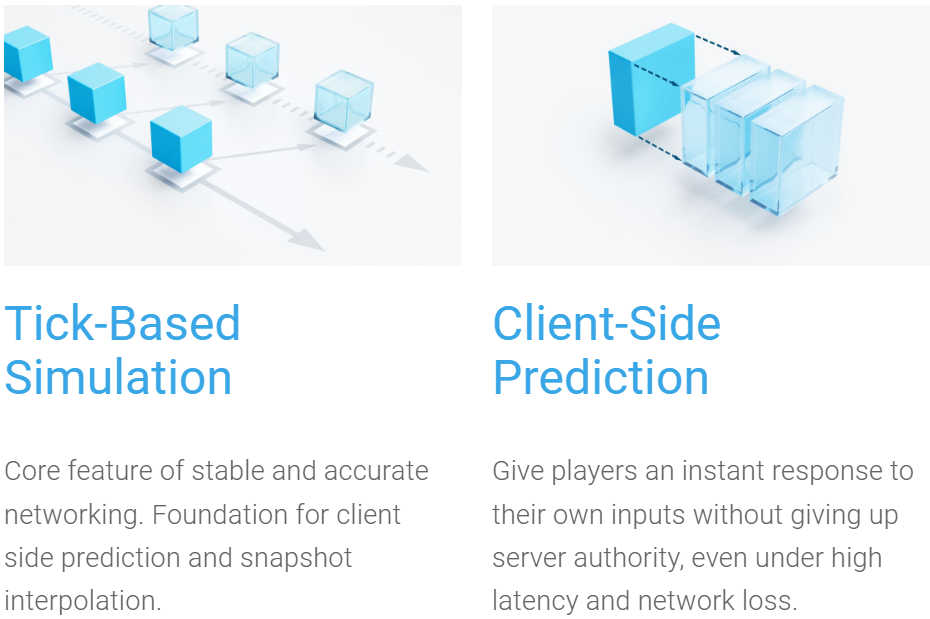
\includegraphics[width=8cm]{4.Cơ sở/images/fusion-1.png}
    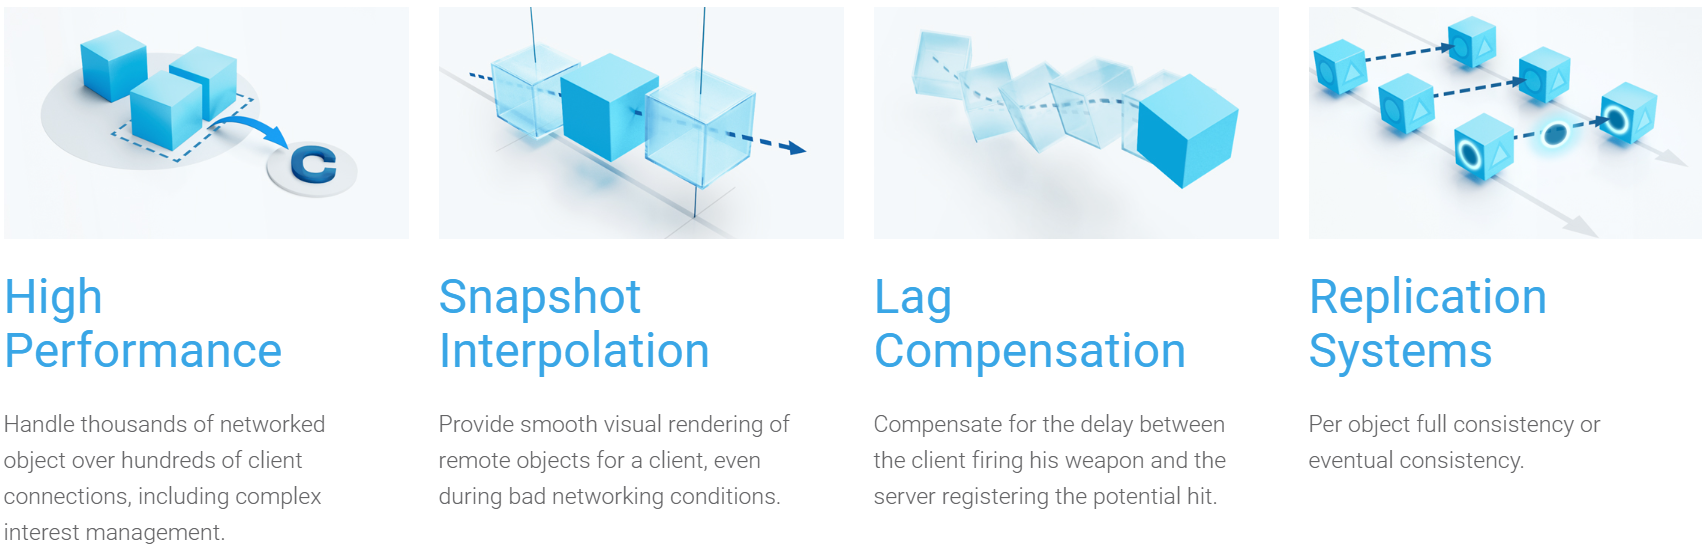
\includegraphics[width=12cm]{4.Cơ sở/images/fusion-2.png}
    \caption{Tính năng chính của Photon Fusion}
    \label{fig:fusion}
    \end{figure}

% Nếu gói subcaption gây lỗi, hãy thử dùng gói subfigure: \usepackage{subfigure}

\begin{figure}[!h]
    \centering
    \begin{minipage}{0.35\textwidth} 
        \centering
        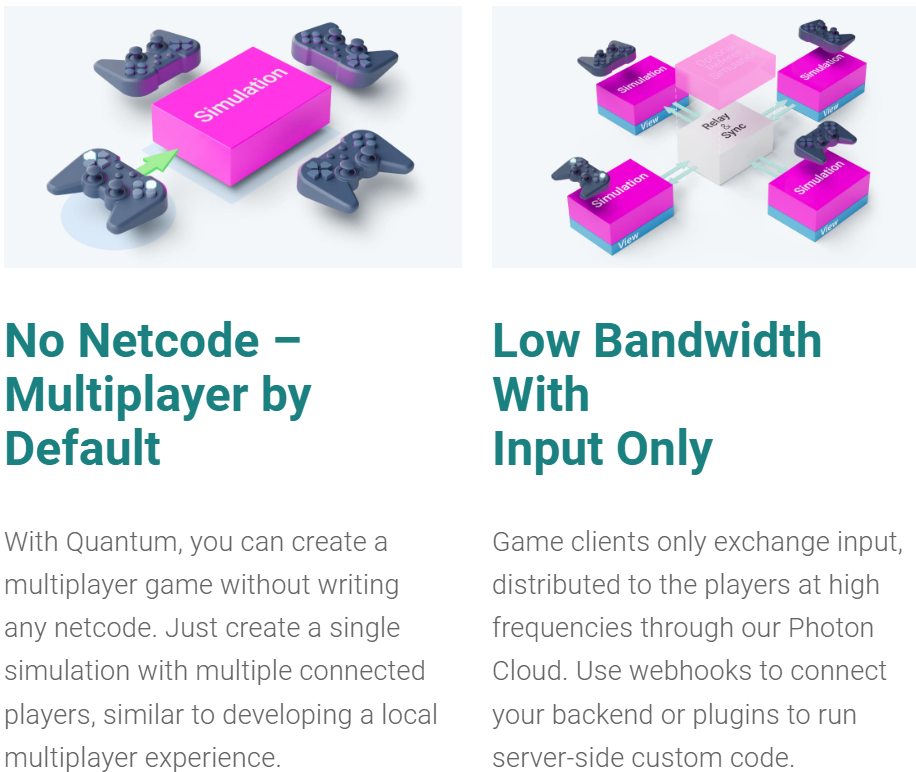
\includegraphics[width=\linewidth]{4.Cơ sở/images/quantum-1.png}
    \end{minipage}
    \begin{minipage}{0.35\textwidth} 
        \centering
        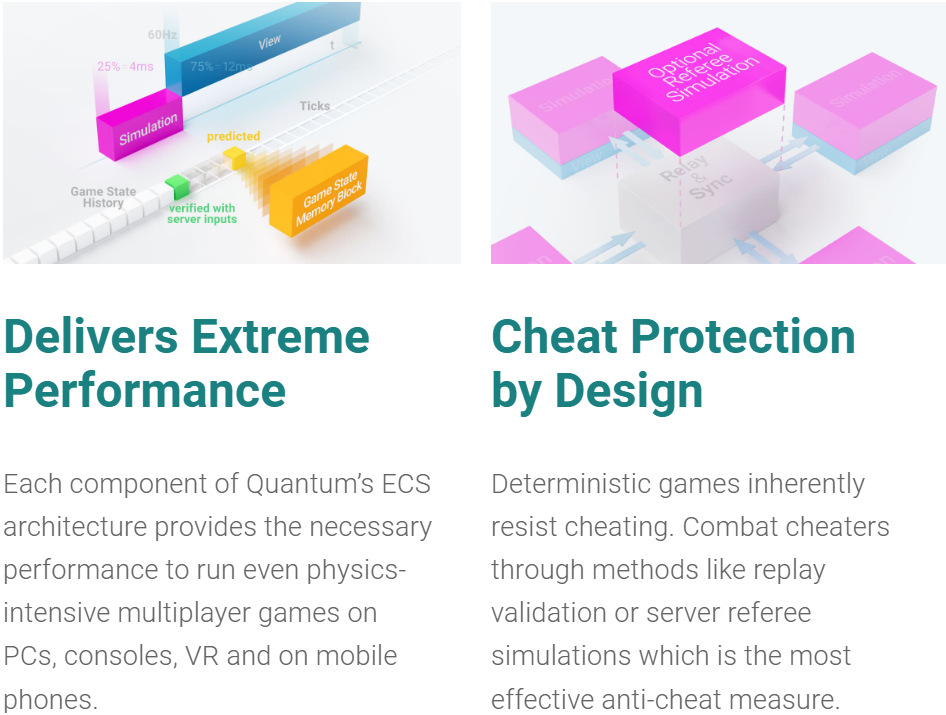
\includegraphics[width=\linewidth]{4.Cơ sở/images/quantum-2.png}
    \end{minipage}
    \centering
    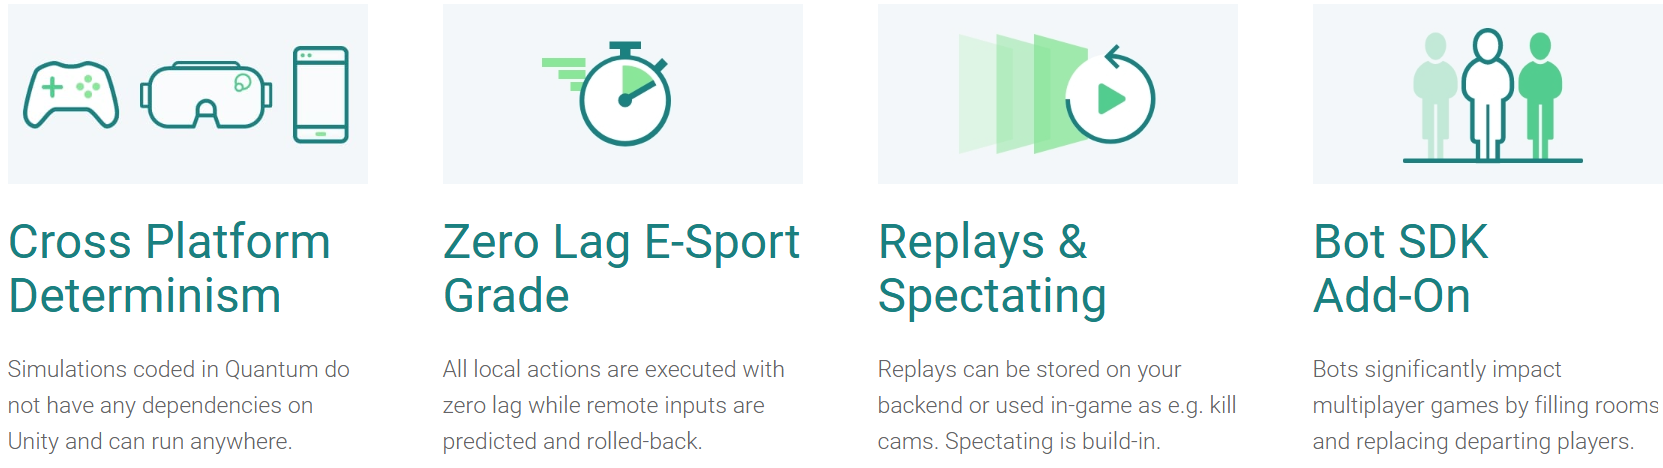
\includegraphics[width=12cm]{4.Cơ sở/images/quantum-3.png}

    \caption{Tính năng chính của Photon Quantum}
    \label{fig:fusion}
\end{figure}
    
    Hiện tại, các giải pháp trên của Photon đều cung cấp gói miễn phí với giới hạn số người dùng trực truyến cùng lúc (CCU) tối đa là 20 và chỉ dành cho phiên bản phát triển (development only). 

    \begin{figure}[!h]
    \centering
    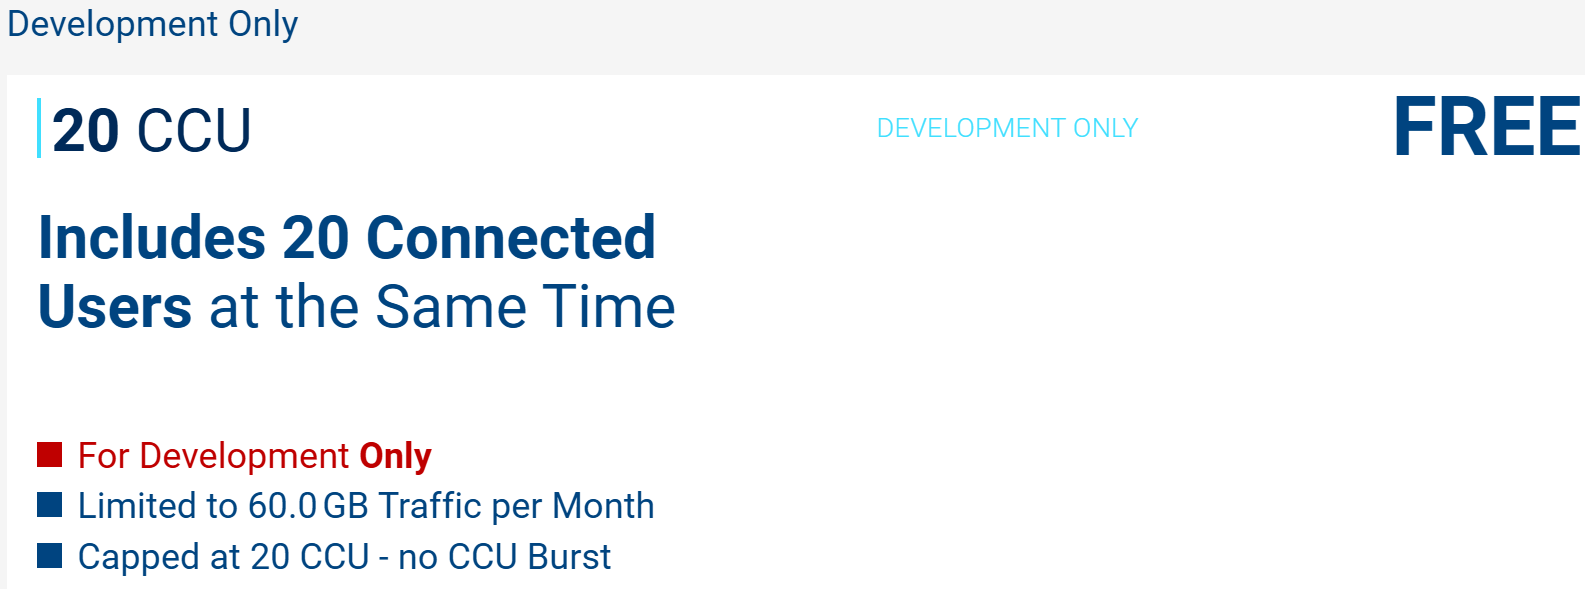
\includegraphics[width=12cm]{4.Cơ sở/images/photon-price-1.png}
    \caption{Gói dịch vụ miễn phí của Photon (PUN, Fusion, Quantum) cho bản phát triển}
    \label{fig:photon-price-1}
    \end{figure}
    
    Riêng công cụ Fusion và Quantum thì có thêm 1 gói miễn phí cho phiên bản phát hành (chỉ 1 app duy nhất) với giới hạn CCU tối đa lên đến 100 kèm theo tăng traffic mỗi tháng (từ 60GB lên 0.3TB).
    \begin{figure}[!h]
    \centering
    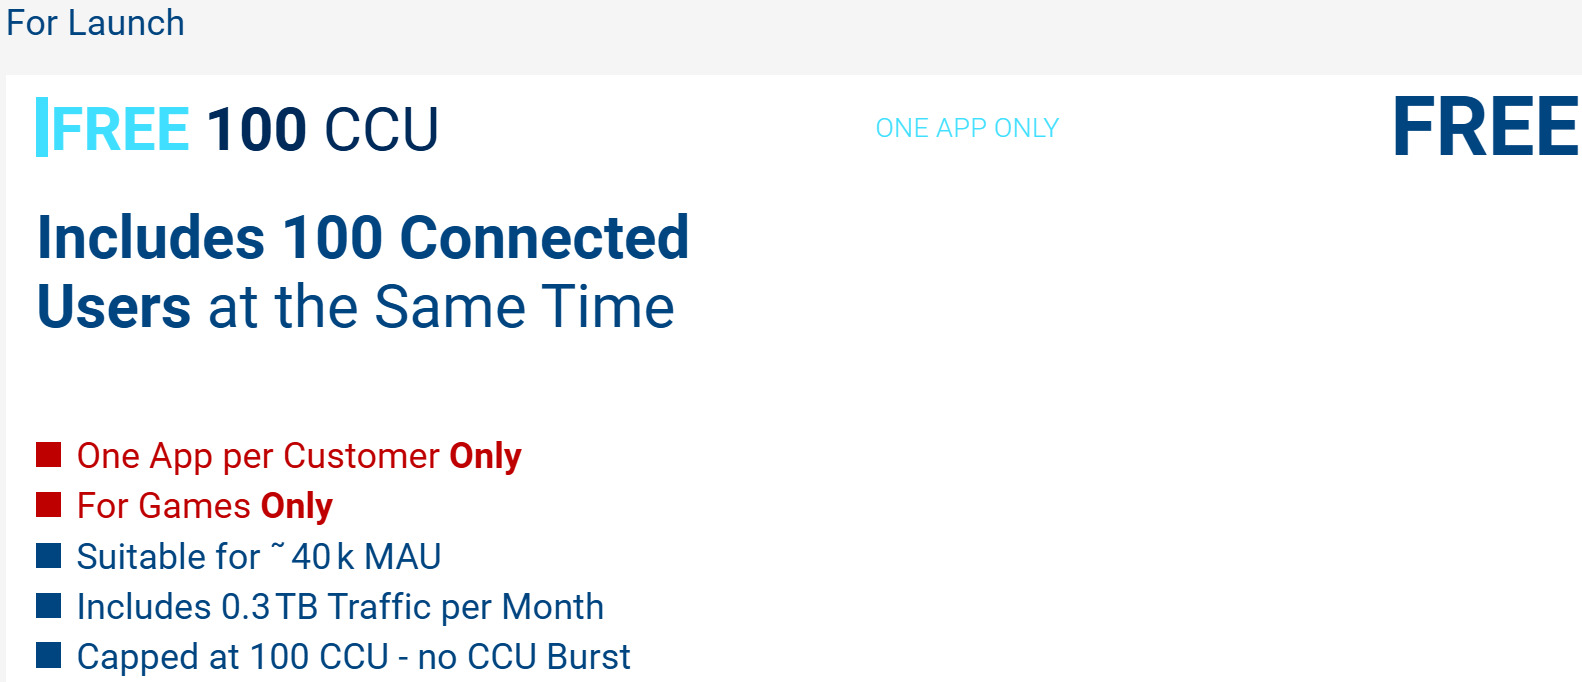
\includegraphics[width=12cm]{4.Cơ sở/images/photon-price-2.png}
    \caption{Gói dịch vụ miễn phí của Photon (Fusion, Quantum) cho bản phát hành}
    \label{fig:photon-price-2}
    \end{figure}
    
    Các gói dịch vụ cao cấp hơn của Photon (mở giới hạn traffic, CCU) phải trả phí (95\$/12 tháng, 125\$/tháng, 250\$/tháng, 500\$/tháng) 
    \begin{figure}[!h]
    \centering
    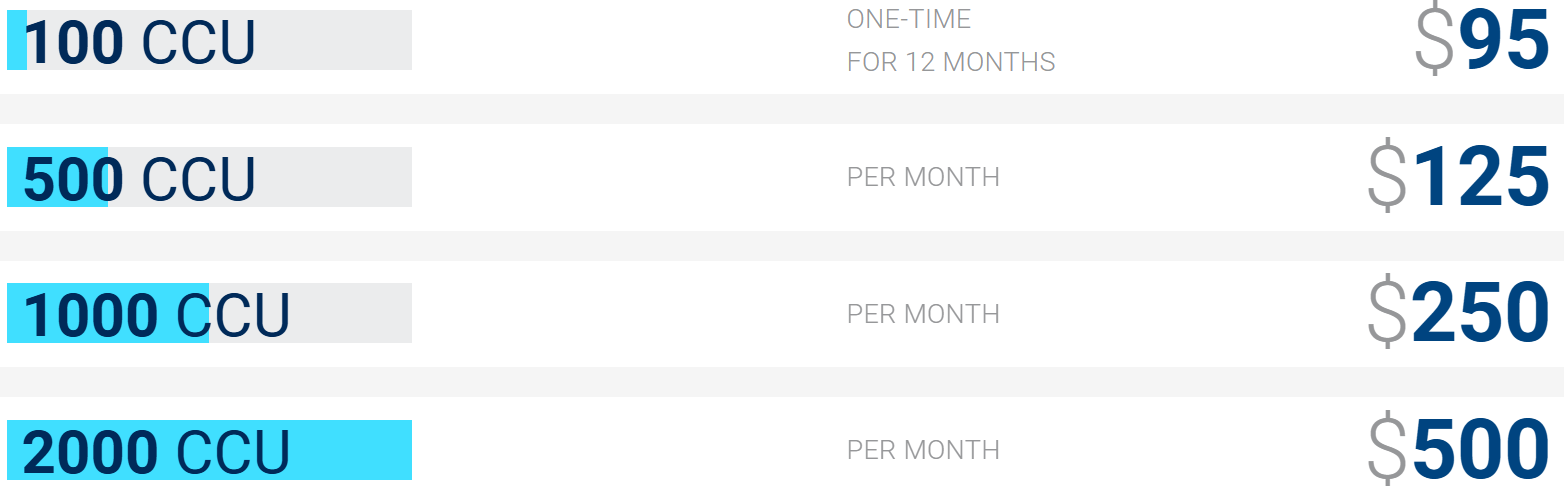
\includegraphics[width=12cm]{4.Cơ sở/images/photon-price-3.png}
    \caption{Gói dịch vụ trả phí của Photon (PUN, Fusion, Quantum)}
    \label{fig:photon-price-3}
    \end{figure}
    
\newpage
\subsubsection{Mirror Networking:}
Mirror Networking là một thư viện mã nguồn mở dùng cho networking trong Unity. Thư viện này hoàn toàn miễn phí và luôn được cập nhật đều đặn đến hiện tại. Mirror Networking hô trợ host mode (P2P) và cả dedicated server. Nhờ những đặc tính của một thư viện mã nguồn mở, công cụ này cung cấp khả năng linh hoạt, tùy biến cao. Điều này phù hợp cho nhóm phát triển nhỏ (indie), yêu cầu cao cho việc kiểm soát logic server, mạng chặt chẽ, mở rộng tùy ý. Giải pháp này không giới hạn về CCU, nhưng sẽ phụ thuộc vào cấu hình server mà nhà phát triển xây dựng.
\subsubsection{Netcode for GameObjects (NGO)}
NGO (Netcode for GameObjects) là một công cụ chính thức được Unity phát triển và là giải pháp mặc định cho quá trình phát triển game Multiplayer trong unity. NGO có giao diện sử dụng dễ dàng, thân thuộc nhờ việc xây dựng trên workflow truyền thống của Unity (GameObject, MonoBehaviour,...). 

Các dịch vụ Multiplayer khác của Unity cũng được tích hợp vào NGO:
\begin{itemize}
    \item Lobby: có thể hỗ trợ lên đến 150 người chơi 1 phòng
    \item Player Authentication: xác thực người dùng đa nền tảng (facebook, google, anonymous,...)
    \item Matchmaker: hỗ trợ cơ chế ghép trận
    \item Relay: hỗ trợ cho P2P
    \item Friends; hỗ trợ cơ chế bạn bè
    \item Vivox: hỗ trợ cơ chế voice chat, text chat
\end{itemize}

NGO hỗ trợ 2 kiến trúc mạng chính là Client-Server (Dedicated server) và Client-Host. Về giao thức truyền tải mạng, NGO sử dụng UPD đạng tin cậy (Reliable UDP), giao thức này vừa kế thừa đặc điểm tốc độ cao của UDP truyền thống, vừa kết hợp đặc tính tin cậy (tính đảm bảo chuyển giao, tính thứ tự) của giao thức TCP.\\

Với gói dịch vụ miễn phí, NGO cung cấp giới hạn CCU tối đa mỗi tháng lên đến 50 và với mỗi mốc vượt ngưỡng sẽ trả phí (pay as you go).
\begin{figure}[!h]
    \centering
    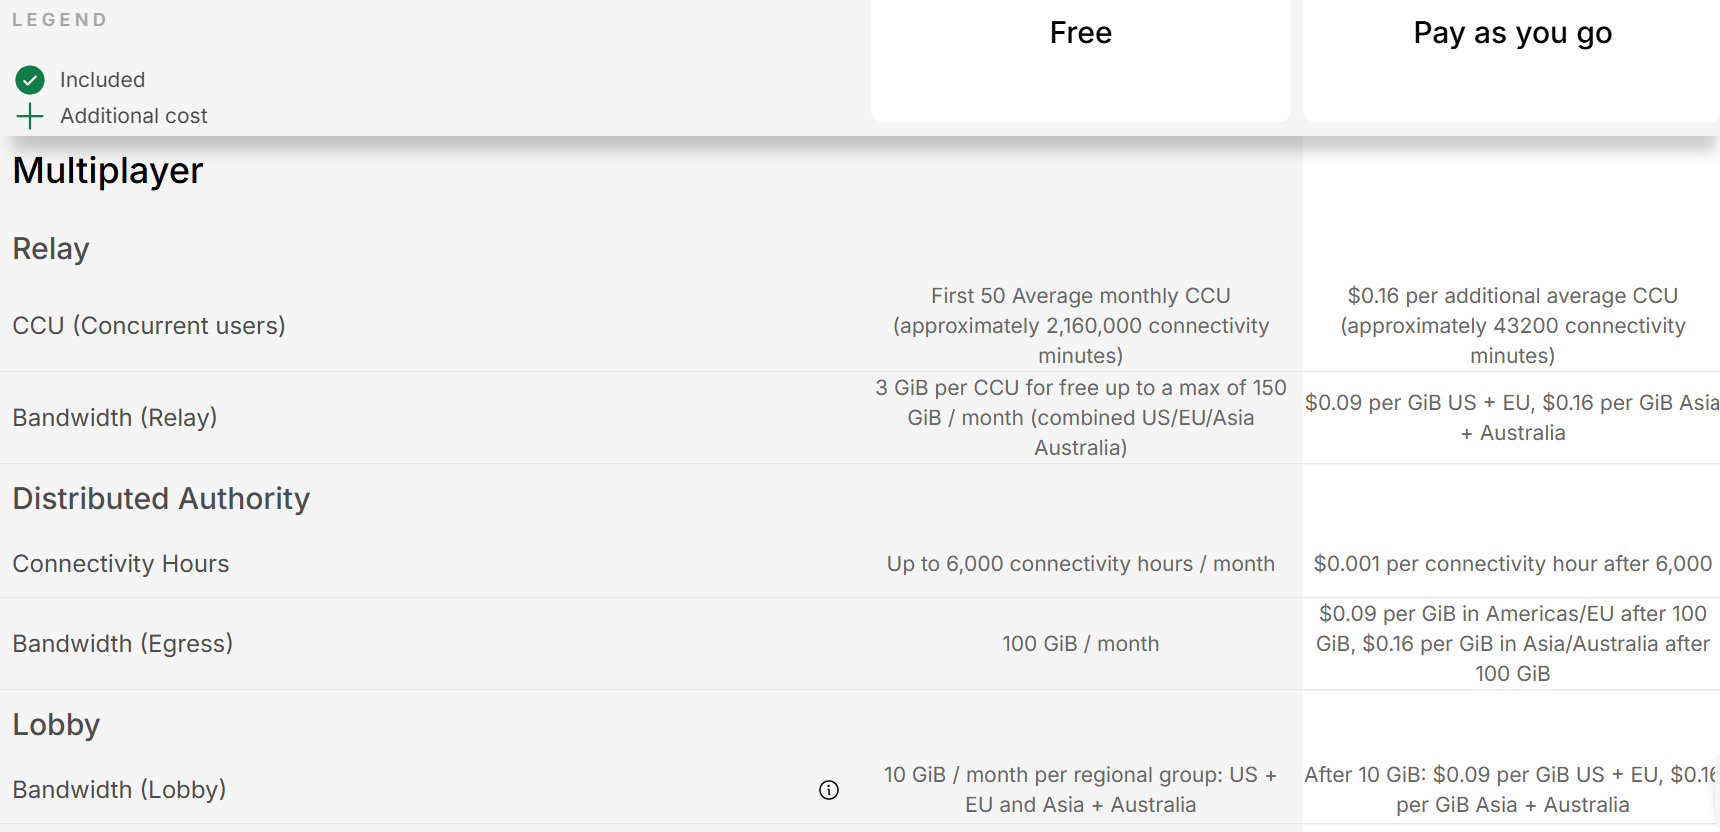
\includegraphics[width=12cm]{4.Cơ sở/images/ngo-price.png}
    \caption{Gói dịch vụ cho Multiplayer của Unity}
    \label{fig:ngo-price}
\end{figure}

Tuy hỗ trợ nhiều dịch vụ, nhưng hệ thống của NGO chỉ phù hợp cho dự án quy mô nhỏ (khoảng 8-16 người chơi 1 phòng). Với các game có số lượng người chơi lớn, hiệu suất của NGO sẽ giảm mạnh. Ngoài ra, NGO cũng không hỗ trợ Client-side Prediction và Lag Compensation, điều này gây khó khăn trong việc hiện thực các game hành động nhanh, FPS khi nhà phát triển phải tự triển khai toàn bộ, làm tăng độ phức tạp của dự án.
\subsubsection{Netcode for Entities}
Tương tự NGO, Netcode for Entities cũng là một công cụ chính thức do Unity phát triển. Tuy nhiên, công cụ này tập trung tối ưu cho những game đòi hỏi số lượng người chơi lớn, xử lý nhiều logic, vật lý cho nhiều vật thể cùng lúc. Netcode for Entities được dùng kết hợp với hệ thống ECS (Entity Component System) và DOTS (Data-Oriented Technology Stack) để tối ưu hiệu suất xử lý đồng thời nhiều đối tượng. Ngoài ra, công cụ này cũng có thể dễ dàng tích hợp với dịch vụ của Unity như NGO.
\subsection{Lý do chọn Unity NGO}
NGO được chọn vì là giải pháp chính thức và khuyến nghị từ Unity, đảm bảo tương thích cao và cập nhật, hỗ trợ thường xuyên. Nó hỗ trợ dễ dàng client-host model, tích hợp với Unity Multiplayer Services (như Relay cho NAT punchthrough), và hiệu suất ổn cho game 3D turn-based. So với Photon, NGO rẻ hơn (dựa trên Unity subscription); so với Mirror, NGO đơn giản hơn cho người mới. So với Netcode for Entities thì NGO đơn giản và phù hợp với dự án hơn, vì kích thước game giới hạn tối đa chỉ là 8 người chơi. Do vậy, NGO là giải pháp tốt nhất về độ phức tạp và chi phí, có thể triển khai dễ dàng cùng như thuận lợi cho việc phát triển các dịch vụ khác của Unity (authentication, voice chat,...).
\subsection{Kiến trúc Network}
Unity Netcode for GameObjects (NGO) cung cấp nhiều mô hình kiến trúc mạng khác nhau nhằm đáp ứng được nhu cầu của từng loại game multiplayer cụ thể. Mô hình kiến trúc mạng sẽ quyết định cách thức mà dữ liệu được truyền đi giữa các máy, việc máy nào sẽ thực thi logic, cũng như tính bảo mật và hiệu suất của hệ thống. NGO sử dụng 2 kiến trúc mạng chính là Client-Server (dedicated server) và Client-Host. Để lựa chọn được kiến trúc mạng phù hợp theo từng giai đoạn của dự án, sau đây nhóm sẽ phân tích tổng quan về hai kiến trúc mạng trên.
\subsubsection{Mô hình Client-Host}
Trong mô hình Client-Host, có một người chơi sẽ lá Host (vừa là Client, vừa là Server) chạy logic Client như những người chơi khác, đồng thời cũng chạy logic của Server. Các người chơi khác là Client sẽ kết nối tới người chơi Host như một kết nối tới Server.
\begin{figure}[H]
    \centering
    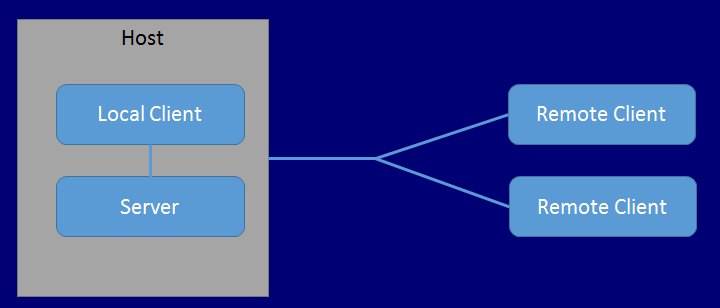
\includegraphics[width=12cm]{4.Cơ sở/images/client-host.png}
    \caption{Mô hình Client-Host}
    \label{fig:ngo-price}
\end{figure}

\begin{itemize}
    \item \textbf{Đặc điẻm chính:}
    \begin{enumerate}[+]
        \item Server ở đây chạy trực tiếp trên máy người chơi (Host).
        \item Không dùng máy chủ riêng.
        \item Máy người chơi Host xử lý toàn bộ logic gameplay và đồng bộ các trạng thái ở máy người chơi client.
    \end{enumerate}
    \item \textbf{Ưu điểm:}
    \begin{enumerate}[+]
        \item Mô hình đơn giản giúp dễ triển khai, phát triển nhanh, phù hợp với game nhỏ.
        \item Không tốn chi phí thuê máy chủ riêng.
    \end{enumerate}
    \item \textbf{Nhược điểm:}
    \begin{enumerate}[+]
        \item Hệ thống phụ thuộc vào cấu hình cũng như mạng của máy Host, máy Host lag thì tất cả người chơi khác đều ảnh hưởng và khi máy Host sập thì game cũng sập.
        \item Tính bảo mật, chống gian lận kém vì người chơi Host quản lý toàn bộ thông tin tất cả người chơi trong phòng và trạng thái gameplay.
    \end{enumerate}
\end{itemize}
\subsubsection{Mô hình Client-Server (Dedicated Server)}
Với mô hình Client-Server, server được chạy trên máy riêng (thường là máy áo), không phải là người chơi. Các người chơi là client sẽ kết nối với server và gửi dữ liệu hoặc gọi lệnh từ server, server sẽ xử lý logic và trả về cho client.
\begin{figure}[!h]
    \centering
    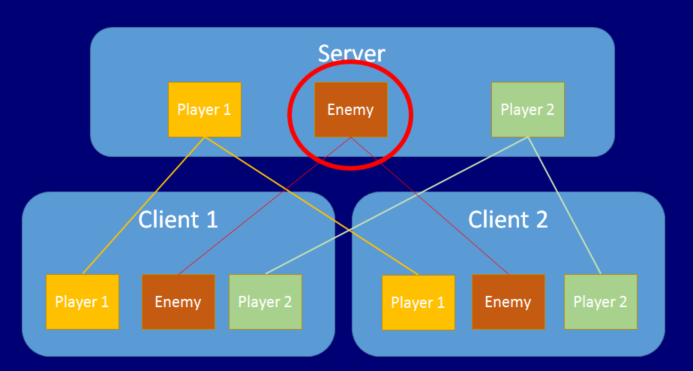
\includegraphics[width=12cm]{4.Cơ sở/images/client-server.png}
    \caption{Mô hình Client-Server (Dedicated Server)}
    \label{fig:client-server}
\end{figure}
\begin{itemize}
    \item \textbf{Đặc điểm chính:}
    \begin{enumerate}[+]
        \item Server là máy chạy độc lập (24/7)
        \item Logic gameplay chỉ được chạy trên server
        \item Client chỉ đóng vai trò hiển thị dữ liệu được server xử lý.
    \end{enumerate}
    \item \textbf{Ưu điểm:} 
    \begin{enumerate}[+]
        \item Tính ổn định cao vì server là máy chạy độc lập, không bị ảnh hưởng bởi người chơi. Người chơi rớt mạng hoặc thoát thì server vẫn chạy.
        \item Tính công bằng, chống gian lận cao do mọi logic và dữ liệu gameplay tập trung ở server, người chơi không có quyền xem dữ liệu người chơi khác cũng như chỉnh sửa dữ liệu gameplay.
        \item Khả năng mở rộng cao khi cần nâng cấp hệ thống (tăng tốc độ truyền, tăng lượng người chơi đồng thời) vì chỉ cần nâng cấp cấu hình máy ảo.
    \end{enumerate}
    \item \textbf{Nhược điểm:} 
    \begin{enumerate}[+]
        \item Tốn chi phí vận hành máy chạy server.
        \item Độ phức tạp cao hơn vì cần có kiến thức về hosting, devops và tối ưu cấu trúc code cho headless server.
    \end{enumerate}
\end{itemize}
\subsubsection{Lý do chọn kiến trúc Client-Host ở giai đoạn phát triển đồ án}
Nhóm quyết định chọn kiến trúc Client-Host cho giai đoạn làm đồ án vì 2 lý do chính là tối ưu tốc độ phát triển dự án và tối ưu về chi phí.
\begin{itemize}
    \item Tối ưu tốc độ phát triển dự án:
    \begin{enumerate}[+]
        \item Kiến trúc Client-Host có thể triển khai dễ dàng trong Unity Editor, không cần triển khai backend, nghiên cứu hosting/devops.
        \item Nhóm phát triền có thể tập trung hơn vào phát triển gameplay, UI của game.
        \item Vì người chơi Host cũng chính là Server nên mỗi lần chơi thử không cần tốn thời gian theo dõi trạng thái server, thuận tiện hơn cho quá trình tìm lỗi.
        \item Giai đoạn phát triển chưa cần quá quan tâm đến độ trễ (không quá ảnh hưởng đến game dạng turn-based) cũng như tính công bằng, bảo mật.
    \end{enumerate}
    \item Tối ưu chi phí: Dự án giai đoạn thử nghiệm ban đầu chưa cần phải thuê dịch vụ máy ảo/hosting nên không tốn chi phí.
\end{itemize}    
\subsubsection{Lý do quyết định chuyển sang kiến trúc Client-Server trong tương lai}
Nhóm dự kiến sẽ chuyển kiến trúc mạng từ Client-Host sang Client-Server trong tương lai, sau khi đã hoàn thiện các logic gameplay cốt lõi và cải tiến UI của game. Mục đính chỉnh của việc này là nhằm tăng chất lượng game về nhiều mặt:
\begin{enumerate}[$\bullet$]
    \item Tính ổn định: Server không còn phụ thuộc vào máy người chơi, điều này giúp cho người chơi có thể ròi phòng bất ký lúc nào (kể cả host) mà không làm gián đoạn game.
    \item Tính công bằng, bảo mật: Chỉ có server mới giữ và xử lý toàn bộ thông tin người chơi và gameplay, người chơi chỉ có quyền xem dữ liệu của bản thân.
    \item Tính mở rộng: Việc xây dựng game trên kiến trúc Client-Server giúp cho nhóm phát triển có thể dễ dàng mở rộng hệ thống game hơn vì khi server không còn là người chơi, việc mở rộng server sẽ trở nên dễ dàng hơn. Các nền tảng phát hành game cũng đòi hỏi điều này đối với các tựa game multiplayer.
\end{enumerate}
\subsection{Giải pháp voice chat Vivox}
Trong các game multiplayer, đặc biệt là dạng board game như nhóm đang triển khai, hệ thống voice chat đóng vai trò rất quan trọng trong việc giúp tăng độ tương tác giữa các người chơi.

Hiện tại trên thị trường có một số giải pháp voice chat có thể tich hợp vào Unity như Vivox, Photon Voice 2, Dissonance Voice và Steam Voice Chat. Sau đây nhóm sẽ đưa ra lý do giải pháp Vivox được chọn để triển khai bằng cách đánh giá tổng quan các giải pháp trên.
\begin{enumerate}[$\bullet$]
    \item \textbf{Vivox:}
    \begin{enumerate}[-]
        \item Miễn phí lên đến tối đa 5000 người dùng hoạt động cùng lúc (5000 PCU)
        \item Được tích hợp trực tiếp trong Unity Service.
        \item API gọn, hỗ trợ channel-based, tùy chỉnh âm lượng theo người chơi.
        \item Chất lượng âm tốt, phù hợp, ổn định với game giải trí.
        \item Hỗ trợ tích hợp thêm text chat nhanh chóng.
    \end{enumerate}
    \item \textbf{Photon Voice 2:}
    \begin{enumerate}[-]
        \item Miễn phí tới 20 CCU (kèm theo của dịch vụ Photon Cloud).
        \item Phù hợp với game dạng realtime (FPS, action).
        \item Overkill với dạng game turn-based, ít hành động.
    \end{enumerate}
    \item \textbf{Dissonance Voice Chat:}
    \begin{enumerate}[-]
        \item Giá công cụ 50 USD (Unity Asset Store).
        \item Chạy local server, tính tùy biến cao.
        \item Phải tự thiết lập backend hoặc tích hợp thủ công với NGO.
        \item Tốt cho dạng game LAN.
    \end{enumerate}
    \item \textbf{Steam Voice Chat:}
    \begin{enumerate}[-]
        \item Miễn phí và ổn định.
        \item Chỉ dùng được cho game phát hành trên Steam.
        \item Không hỗ trợ chia channel dễ dàng như Vivox.
    \end{enumerate}
\end{enumerate}

Từ các đặc điểm trên, Vivox là giải pháp tốt nhất không chỉ về chi phí, tính năng mà còn về phù hợp nhất với thể loại game và phù hợp cả với hệ thông NGO mà nhóm đã chọn trước đó. Do đó, nhóm chọn sử dụng Vivox để phát triển hệ thống voice chat và text chat trong game.
\subsection{Design Pattern trong dự án}
\subsubsection{Singleton}

Singleton là một trong những mẫu thiết kế phổ biến nhất trong phát triển game, đặc biệt trong Unity. Mẫu này đảm bảo chỉ tồn tại duy nhất một thể hiện (\textit{instance}) của một lớp trong suốt vòng đời ứng dụng, đồng thời cung cấp điểm truy cập toàn cục tới thể hiện đó. Singleton thường được sử dụng cho các hệ thống quan trọng như \texttt{GameManager}, \texttt{AudioManager}, \texttt{UIManager} hoặc \texttt{NetworkManager}.

\begin{enumerate}[$\bullet$]
    \item{\textbf{Ưu điểm:}}
    \begin{enumerate}[+]
    \item \textbf{Dễ truy cập và tiện lợi:} Mọi thành phần trong game có thể dễ dàng lấy instance thông qua thuộc tính tĩnh, ví dụ \texttt{GameManager.Instance}, giảm nhu cầu truyền tham chiếu.
    \item \textbf{Đảm bảo tính duy nhất:} Ngăn chặn việc tạo nhiều đối tượng quản lý gây xung đột tài nguyên hoặc trạng thái.
    \item \textbf{Phù hợp cho các hệ thống global:} Các hệ thống cần tồn tại xuyên suốt nhiều scene có thể hoạt động ổn định nhờ \texttt{DontDestroyOnLoad}.
    \item \textbf{Dễ triển khai:} Chỉ cần cấu trúc đơn giản, thuận lợi cho cả lập trình viên mới.
\end{enumerate}
\newpage
\item{\textbf{Nhược điểm:}}
\begin{enumerate}[+]
    \item \textbf{Tạo ra Global State:} Việc quản lý trạng thái toàn cục khiến quá trình debug khó khăn hơn và dễ phát sinh lỗi không lường trước.
    \item \textbf{Tăng sự phụ thuộc (tight coupling):} Các lớp trong hệ thống dễ bị phụ thuộc trực tiếp vào Singleton, dẫn đến kiến trúc kém linh hoạt.
    \item \textbf{Khó khăn trong Unit Testing:} Singleton sử dụng trạng thái tĩnh, khiến việc reset hoặc mock dữ liệu trở nên phức tạp.
    \item \textbf{Dễ bị lạm dụng:} Việc dùng Singleton không hợp lý có thể phá vỡ tính module hóa và vi phạm nguyên tắc thiết kế SOLID.
    \item \textbf{Vấn đề cạnh tranh tài nguyên (concurrency):} Trong môi trường multiplayer hoặc multithread, Singleton cần cơ chế đồng bộ để tránh lỗi race condition.
\end{enumerate}
\end{enumerate}


% Singleton đảm bảo chỉ có một instance của class, cung cấp global access. Trong Unity, áp dụng cho GameManager để quản lý state game (score, level). Implement: Private constructor, static instance. Ưu điểm: Dễ truy cập, tránh duplicate. Nhược điểm: Khó test, có thể gây global state issues.

\subsubsection{Observer Pattern}

Observer Pattern là một mẫu thiết kế hành vi cho phép nhiều đối tượng (\textit{observers}) đăng ký và theo dõi sự thay đổi từ một nguồn phát (\textit{subject}). Khi trạng thái của \textit{subject} thay đổi, tất cả các \textit{observers} sẽ tự động được thông báo và cập nhật theo. Phương pháp này giúp loại bỏ sự phụ thuộc chặt chẽ giữa các đối tượng và mang lại khả năng mở rộng linh hoạt, đặc biệt trong những hệ thống có nhiều thành phần cần phản ứng đồng bộ với dữ liệu hoặc sự kiện.

Trong phát triển game bằng Unity, Observer Pattern trở nên đặc biệt hiệu quả nhờ kiến trúc dựa trên \texttt{ScriptableObject} theo khuyến nghị trong bài trình bày \textit{“Game Architecture with Scriptable Objects”} tại Unite Austin 2017 \cite{hipple2017}. Thay vì để các GameObject gọi trực tiếp lẫn nhau hoặc tạo chuỗi tham chiếu phức tạp, Unity có thể sử dụng các \textit{Event Channels}—một dạng ScriptableObject đóng vai trò trung gian. Các hệ thống khác nhau (UI, gameplay, NPC, player controller, animation, v.v.) chỉ cần đăng ký lắng nghe các sự kiện được phát ra từ một Event Channel, mà không cần biết đối tượng nào đã gửi sự kiện.

Cách tiếp cận này mang lại nhiều ưu điểm:
\begin{itemize}
    \item \textbf{Giảm phụ thuộc (decoupling)} giữa các hệ thống: sender và receiver không cần tham chiếu trực tiếp đến nhau.
    \item \textbf{Dễ mở rộng và bảo trì}: thêm hoặc bỏ một observer không ảnh hưởng luồng xử lý.
    \item \textbf{Tái sử dụng logic}: cùng một sự kiện có thể được nhiều hệ thống lắng nghe, như UI cập nhật thông tin, hiệu ứng âm thanh, hoặc logic gameplay.
    \item \textbf{Thân thiện với workflow của Unity}: ScriptableObject sống độc lập với scene, giúp các sự kiện có thể dùng chung xuyên suốt toàn bộ trò chơi.
\end{itemize}

Với dự án, Observer Pattern được ứng dụng vào nhiều cơ chế như: truyền sự kiện thay đổi trạng thái người chơi, thông báo khi người chơi tương tác đồ vật, cập nhật UI theo hành động trong Cabin, hay đồng bộ các sự kiện bắt đầu/thoát khỏi bàn board game. Nhờ sử dụng Event Channels, các thành phần trong game chỉ cần đăng ký lắng nghe sự kiện (OnGameStart, OnSitDown, OnInteractObject, \ldots) mà không cần duy trì quan hệ tham chiếu phức tạp giữa các script.

Áp dụng Observer Pattern theo phương pháp từ Unite Austin 2017 giúp kiến trúc của trò chơi gọn gàng hơn, dễ mở rộng và ít lỗi hơn, đồng thời phù hợp với quy mô một dự án nhiều người chơi, nơi các hệ thống UI, network, hành vi nhân vật và bàn board game cần được đồng bộ và hoạt động trơn tru.

\begin{lstlisting}[style=csharpstyle, caption={Event Channel trong dự án}]
using UnityEngine;
using UnityEngine.Events;

/// <summary>
/// This class is used for Events that have no arguments (Example: Start game event)
/// </summary>
[CreateAssetMenu(menuName = "Events/Void Event Channel")]
public class VoidEventChannelSO : ScriptableObject
{
    public UnityAction OnEventRaised = delegate { };

    public void RaiseEvent() => OnEventRaised.Invoke();
}
\end{lstlisting}


% Observer cho phép objects subscribe/unsubscribe để nhận notify khi state thay đổi, decoupling components. Trong Unity, dùng cho event system như player death notify UI update. Implement qua UnityEvent hoặc custom. Ưu điểm: Loose coupling, dễ mở rộng.
\subsubsection{State Pattern}

State Pattern là một mẫu thiết kế quan trọng trong phát triển game hiện đại, được trình bày rõ trong cuốn \textit{Game Programming Algorithms and Techniques}\cite{madhav2013}. Mục tiêu của mẫu thiết kế này là quản lý hành vi của một thực thể thông qua nhiều trạng thái khác nhau mà không cần sử dụng các cấu trúc điều kiện phức tạp như \texttt{if-else} hoặc \texttt{switch-case}. \\

Thay vào đó, mỗi trạng thái được tách thành một lớp độc lập, chịu trách nhiệm cho ba giai đoạn vòng đời chính: \textbf{OnEnter}, \textbf{OnTick} và \textbf{OnExit}. Cách tiếp cận này mang lại nhiều lợi ích: mã nguồn rõ ràng và dễ bảo trì, hành vi được tách bạch theo trạng thái, dễ mở rộng thêm trạng thái mới và dễ dàng kiểm soát quá trình chuyển đổi giữa các trạng thái.\\

Trong dự án, người chơi có nhiều trạng thái khác nhau như \textit{Idle}, \textit{Move}, \textit{Jump}, \textit{Sit}, v.v. Mỗi trạng thái được xây dựng dựa trên interface \texttt{IState} để đảm bảo cấu trúc nhất quán và dễ dàng quản lý.

\newpage 
\begin{lstlisting}[style=csharpstyle, caption={Interface IState trong dự án}]
public interface IState
{
    public void OnEnter();
    public void OnTick();
    public void OnExit();
}
\end{lstlisting}

Interface trên định nghĩa một quy tắc chung cho tất cả các trạng thái. Mọi trạng thái mới đều phải thực hiện ba phương thức này, từ đó đảm bảo rằng vòng đời của trạng thái được tuân thủ chặt chẽ.

\begin{lstlisting}[style=csharpstyle, caption={Ví dụ: IdleState}]
public class IdleState : IState
{
    protected Animator _animator;
    protected PlayerController _host;   
    protected static readonly int _animHash = Animator.StringToHash("Idle");

    public IdleState(PlayerController host, Animator animator)
    {
        _host = host;
        _animator = animator;
    }

    public virtual void OnEnter()
    {
        _animator.Play(_animHash);
        _host.Movement = Vector3.zero;
    }

    public virtual void OnExit() { }

    public virtual void OnTick() { }
}
\end{lstlisting}

Ví dụ trên mô tả trạng thái \textit{Idle}. Khi bước vào trạng thái này, nhân vật sẽ phát animation đứng yên và đặt vector chuyển động về 0. Trạng thái tự quản lý hành vi của nó, không gây ảnh hưởng đến các trạng thái khác, đúng theo tinh thần của State Pattern.

\begin{lstlisting}[style=csharpstyle, caption={Hàm chuyển trạng thái trong State Machine}]
private void ToState(IState newState)
{
    if (_currentState == newState) return;
    _currentState.OnExit();
    _currentState = newState;
    _currentState.OnEnter();
}
\end{lstlisting}

Hàm \texttt{ToState} là trung tâm của hệ thống State Machine: đảm bảo quá trình thoát khỏi trạng thái cũ và khởi tạo trạng thái mới được thực hiện đúng thứ tự. Đồng thời, việc gọi \texttt{OnTick} mỗi khung hình sẽ giúp trạng thái hiện tại xử lý logic của nó một cách độc lập.

\begin{lstlisting}[style=csharpstyle, caption={Hàm Update trong game loop}]
void Update()
{
    if (!IsOwner)
        return;
    _currentState.OnTick();
}
\end{lstlisting}

Tổng kết lại, việc áp dụng State Pattern giúp hệ thống điều khiển nhân vật trong dự án trở nên linh hoạt, dễ mở rộng, rõ ràng và ít lỗi hơn, phù hợp với kiến trúc được khuyến nghị trong tài liệu của Sanjay Madhav.

% Dựa theo giải pháp State Pattern trong cuốn sách Game Programming Algorhitms and Techniques của tác giả Sanjay Madhav


% State pattern cho phép object thay đổi behavior khi state thay đổi, như player states (idle, running, jumping). Strategy tương tự nhưng cho algorithms interchangeable, như AI behaviors (patrol, attack). Trong dự án, dùng cho player controller và enemy AI. Ưu điểm: Clean code, dễ maintain.


\newpage
\section{Đặc tả chi tiết các lược đồ}
\subsection{Thiết kế chi tiết các use-case và kịch bản}
\subsubsection{Tổng quan}
Sơ đồ use-case \textbf{màn hình chính}:
\begin{figure}[H]
    \centering
    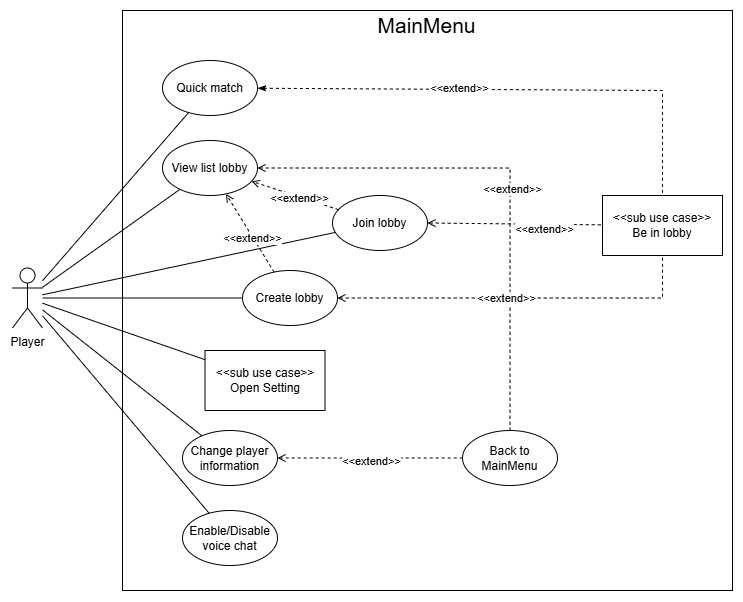
\includegraphics[width=0.75\linewidth]{4.Đặc tả chi tiết các lược đồ/Use-case/images/MainMenu.png}
    \caption{Use-case mô tả màn hình chính}
    \label{fig:placeholder}
\end{figure}

Người chơi có thể chỉnh sửa thông tin cá nhân, vào phòng chơi bằng cách chọn phòng hoặc tạo phòng hoặc vào phòng nhanh (quick match). Cùng với đó còn có các chức năng khác người dùng có thể thực hiện trong các use-case phụ trong use-case màn hình chính, cụ thể use-case bao gồm các use-case phụ sau:
\begin{itemize}
    \item \textbf{Mở cài đặt}: Tại đây sẽ dẫn người chơi vào use-case Settings, use-case này mô tả các hoạt động có thể thực hiện được khi mở cài đặt.
    \item \textbf{Trong phòng}: tại đây  sẽ dẫn người chơi vào use-case In Lobby, use-case này mô tả các hoạt động có thể thực hiện được khi vào đã vào trong lobby.
\end{itemize}
\subsubsection{Trong lobby}
Sơ đồ use-case trong lobby:
\begin{figure}[H]
    \centering
    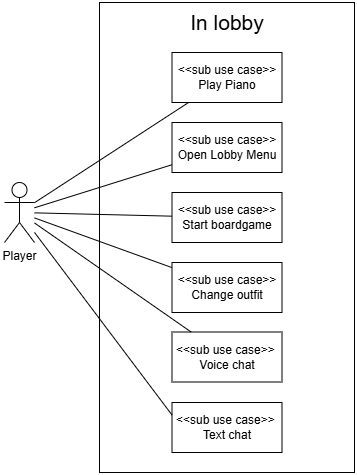
\includegraphics[width=0.75\linewidth]{4.Đặc tả chi tiết các lược đồ/Use-case/images/InLobby.png}
    \caption{Use-case mô tả trong lobby}
    \label{fig:placeholder}
\end{figure}
Người chơi có thể thực hiện các use-case phụ trong use-case trong lobby, cụ thể use-case bao gồm các use-case phụ sau:
\begin{itemize}
    \item \textbf{Chơi đàn piano}: Tại đây sẽ dẫn người chơi vào use-case Play Piano, use-case này mô tả các hoạt động cần thiết để có thể chơi được đàn piano.
    \item \textbf{Mở Lobby menu}: Tại đây sẽ dẫn người chơi vào use-case LobbyMenu, use-case này mô tả các các khả năng của người chơi khi mở Lobby Menu, bao gồm kick người chơi khác, xem thông tin phòng, ...
    \item \textbf{Bắt đầu chơi boardgame}: Tại đây sẽ dẫn người chơi vào use-case Play BoardGame, use-case này mô tả các hoạt động cần thiết để có thể vào chơi được boardgame.
    \item \textbf{Thay đổi trang phục}: Tại đây sẽ dẫn người chơi vào use-case Change Outfit, use-case này mô tả các bước cần thực hiện để có thể thay đổi được trang phục.
    \item \textbf{Voice chat}: Tại đây sẽ dẫn người chơi vào use-case Voice chat, use-case này mô tả các bước cần thực hiện để có thể sử dụng voice chat.
    \item \textbf{Text chat}: Tại đây sẽ dẫn người chơi vào use-case Text chat, use-case này mô tả các bước cần thực hiện để có thể sử dụng text chat.
\end{itemize}
\subsubsection{Lobby Menu}
Sơ đồ use-case Lobby Menu:
\begin{figure}[H]
    \centering
    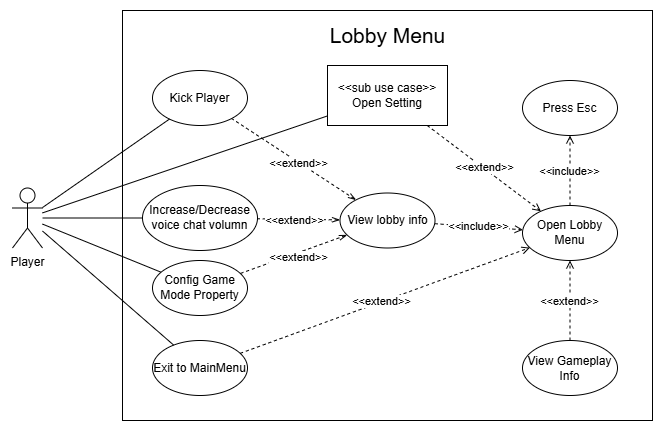
\includegraphics[width=0.75\linewidth]{4.Đặc tả chi tiết các lược đồ/Use-case/images/LobbyMenu.png}
    \caption{Use-case mô tả Lobby Menu}
    \label{fig:placeholder}
\end{figure}


\begin{table}[H]
\centering
\begin{tabular}{|p{4cm}|p{10cm}|}
\hline
\textbf{Use-case name} & Lobby Menu \\ \hline
\textbf{Actor} & Người chơi \\ \hline
\textbf{Descriptions} & Use-case này sẽ chỉ ra các luồng thực thi sau khi mở Lobby Menu. \\ \hline
\textbf{Pre-conditions} & Phải vào được trong lobby \\ \hline
\textbf{Trigger} & Người chơi nhấn nút “Esc” sau khi đã vào lobby. \\ \hline
\textbf{Post-conditions} & Người chơi chọn hành động mà mình muốn thực hiện \\ \hline
\textbf{Normal Flow} &
\begin{enumerate}
\item Người chơi nhấn nút \textbf{"Esc"} mở Lobby Menu.
\item Người chơi chọn các hành động player muốn.
\item Người chơi nhấn nút \textbf{"Esc"} để đóng Lobby Menu
\item Use-case kết thúc sau khi Lobby Menu được đóng thành công.
\end{enumerate}
\\ \hline
\textbf{Alternative Flow} &
\begin{enumerate}
\item[A1.] Sau khi mở được Lobby Menu, nếu người chơi muốn kick player khác thì người chơi nhấn "LOBBY INFO" sau đó chọn người chơi muốn kick và nhấn dấu x (chỉ chủ phòng mới có thể kick).
\item[A2.] Sau khi mở được Lobby Menu, nếu người chơi muốn Tăng/giảm âm lượng voice thì người chơi nhấn "LOBBY INFO", sau đó người tăng/giảm âm lượng voice chat của người chơi khác hoặc chính mình.
\item[A3.] Sau khi mở được Lobby Menu, nếu người chơi muốn điều chỉnh thông số của game mode thì người chơi nhấn "LOBBY INFO", sau đó nhấn nút nút mũi tên ">" rồi chọn game mode và điều chỉnh thông số của mode đó.
\item[A4.] Sau khi mở được Lobby Menu, nếu người chơi muốn thoát ra màn hình chính (rời khỏi phòng) thì người chơi nhấn nút "LEAVE GAME".
\item[A5. ] Sau khi mở được Lobby Menu, nếu người chơi muốn mở setting thì người chơi nhấn nút "SETTINGS".
\end{enumerate}
\\ \hline
\textbf{Exception Flow} &
Không có
\\ \hline
\end{tabular}
\end{table}
\subsubsection{Start Board Game}
Sơ đồ use-case Start Board Game:
\begin{figure}[H]
    \centering
    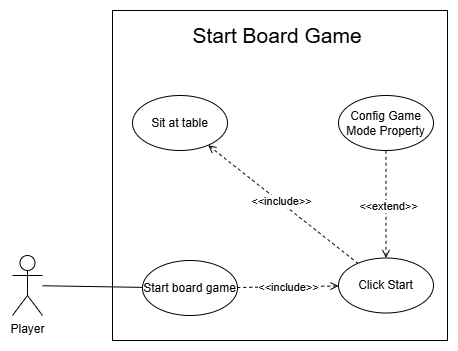
\includegraphics[width=0.75\linewidth]{4.Đặc tả chi tiết các lược đồ/Use-case/images/StartBoardGame.png}
    \caption{Use-case mô tả Start Board Game}
    \label{fig:placeholder}
\end{figure}


\begin{table}[H]
\centering
\begin{tabular}{|p{4cm}|p{10cm}|}
\hline
\textbf{Use-case name} & Start Board Game \\ \hline
\textbf{Actor} & Người chơi \\ \hline
\textbf{Descriptions} & Use-case này sẽ chỉ ra các bước cần thực hiện để có thể chơi được board game. \\ \hline
\textbf{Pre-conditions} & Phải vào được trong lobby \\ \hline
\textbf{Trigger} & Người chơi nhấn nút “Start” sau khi đã ngồi vào bàn và có từ 3 người chơi đang ngồi. \\ \hline
\textbf{Post-conditions} & Không có \\ \hline
\textbf{Normal Flow} &
\begin{enumerate}
\item Người chơi di chuyển đến ghế trống quanh bàn.
\item Người chơi nhấn giữ \textbf{''F''} để ngồi vào bàn.
\item Người chơi nhấn Start để bắt đầu vào game.
\end{enumerate}
\\ \hline
\textbf{Alternative Flow} &
\begin{enumerate}
\item[A1.] Trước bước 3, người chơi có thể chọn game mode và điều chỉnh thông số cần thiết của game mode đó.
\end{enumerate}
\\ \hline
\textbf{Exception Flow} &
\begin{enumerate}
\item[E1.] Tại bước 2, nếu bàn đang chơi thì không thể ngồi vào được
\item[E2.] Tại bước 3, nếu không đủ số người chơi đang ngồi thì không thể nhấn nút Start được.
\end{enumerate}
\\ \hline
\end{tabular}
\end{table}
\subsubsection{Setting}
Sơ đồ use-case Setting:
\begin{figure}[H]
    \centering
    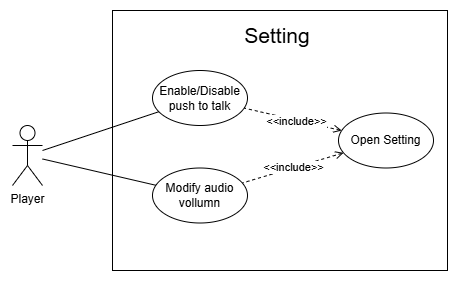
\includegraphics[width=0.75\linewidth]{4.Đặc tả chi tiết các lược đồ/Use-case/images/Setting.png}
    \caption{Use-case mô tả Setting}
    \label{fig:placeholder}
\end{figure}


\begin{table}[H]
\centering
\begin{tabular}{|p{4cm}|p{10cm}|}
\hline
\textbf{Use-case name} & Setting \\ \hline
\textbf{Actor} & Người chơi \\ \hline
\textbf{Descriptions} & Use-case này sẽ chỉ ra các luồng thực thi sau khi mở Setting. \\ \hline
\textbf{Pre-conditions} & Không có \\ \hline
\textbf{Trigger} & Người chơi nhấn nút “SETTINGS” sau khi đã vào lobby hoặc bên ngoài MainMenu. \\ \hline
\textbf{Post-conditions} & Người chơi chọn hành động mà mình muốn thực hiện \\ \hline
\textbf{Normal Flow} &
\begin{enumerate}
\item Nếu đang ở trong lobby thì mở Lobby Menu và nhấn nút "SETTINGS", còn nếu đang ở MainMenu thì chỉ cần nhấn nút "SETTINGS".
\item Người chơi điều chỉnh các thông số.
\item Người chơi nhấn nút "Back" để đóng Setting
\item Use-case kết thúc sau khi Setting được đóng thành công.
\end{enumerate}
\\ \hline
\textbf{Alternative Flow} &
\begin{enumerate}
\item[A1.] Sau khi mở được Setting, nếu người chơi muốn tắt/bật mic của chính mình thì tick vào mục Push-to-talk và nhấn "Save" để lưu.
\item[A2.] Sau khi mở được Setting, nếu người chơi muốn tăng/giảm âm lượng thì kéo slider của mục "Music Volumn" hoặc "Sfx Volumn" tương ứng và nhấn "Save" để lưu.
\end{enumerate}
\\ \hline
\textbf{Exception Flow} &
Không có
\\ \hline
\end{tabular}
\end{table}
\subsubsection{Change outfit}
Sơ đồ use-case Change outfit:
\begin{figure}[H]
    \centering
    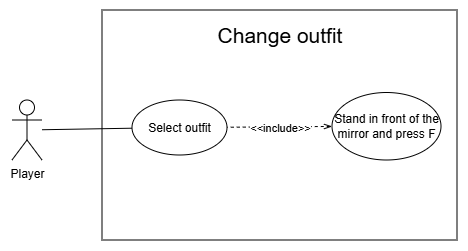
\includegraphics[width=0.75\linewidth]{4.Đặc tả chi tiết các lược đồ/Use-case/images/ChangeOutfit.png}
    \caption{Use-case mô tả Change outfit}
    \label{fig:placeholder}
\end{figure}


\begin{table}[H]
\centering
\begin{tabular}{|p{4cm}|p{10cm}|}
\hline
\textbf{Use-case name} & Change outfit \\ \hline
\textbf{Actor} & Người chơi \\ \hline
\textbf{Descriptions} & Use-case này sẽ chỉ ra các bước cần thực hiện để có thể thay đổi trang phục. \\ \hline
\textbf{Pre-conditions} & Phải vào được trong lobby \\ \hline
\textbf{Trigger} & Không có. \\ \hline
\textbf{Post-conditions} & Không có \\ \hline
\textbf{Normal Flow} &
\begin{enumerate}
\item Người chơi di chuyển đến trước gương.
\item Người chơi nhấn giữ \textbf{''F''} để vào trang thái thay trang phục.
\item Người chơi chọn trang phục mình muốn bằng cách nhấn các mũi tên tương ứng với loại trang phục.
\item Người chơi nhấn giữ \textbf{''F''} để thoát trạng thái thay trang phục.
\item Use-case kết thúc sau khi người chơi thoát trạng thái thay trang phục.
\end{enumerate}
\\ \hline
\textbf{Alternative Flow} &
Không có
\\ \hline
\textbf{Exception Flow} &
Không có
\\ \hline
\end{tabular}
\end{table}
\subsubsection{Play Piano}
Sơ đồ use-case Play Piano:
\begin{figure}[H]
    \centering
    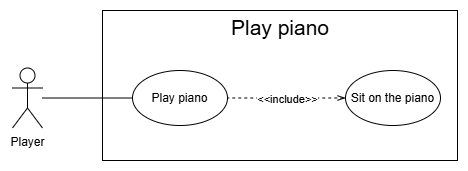
\includegraphics[width=0.75\linewidth]{4.Đặc tả chi tiết các lược đồ/Use-case/images/PlayPiano.png}
    \caption{Use-case mô tả Play Piano}
    \label{fig:placeholder}
\end{figure}


\begin{table}[H]
\centering
\begin{tabular}{|p{4cm}|p{10cm}|}
\hline
\textbf{Use-case name} & Play Piano \\ \hline
\textbf{Actor} & Người chơi \\ \hline
\textbf{Descriptions} & Use-case này sẽ chỉ ra các bước cần thực hiện để có thể chơi đàn piano. \\ \hline
\textbf{Pre-conditions} & Phải vào được trong lobby \\ \hline
\textbf{Trigger} & Không có. \\ \hline
\textbf{Post-conditions} & Không có \\ \hline
\textbf{Normal Flow} &
\begin{enumerate}
\item Người chơi di chuyển đến trước ghế ở piano.
\item Người chơi nhấn giữ \textbf{''F''} để ngồi vào ghế.
\item Người chơi bắt đầu chơi đàn bằng cách nhấn 7 phím đầu tiên của 3 hàng trên bàn phím.
\item Người chơi nhấn giữ \textbf{''F''} để đứng dậy.
\item Use-case kết thúc sau khi người chơi đứng dậy.
\end{enumerate}
\\ \hline
\textbf{Alternative Flow} &
Không có
\\ \hline
\textbf{Exception Flow} &
Không có
\\ \hline
\end{tabular}
\end{table}
\subsubsection{Voice Chat}
Sơ đồ use-case Voice chat:
\begin{figure}[H]
    \centering
    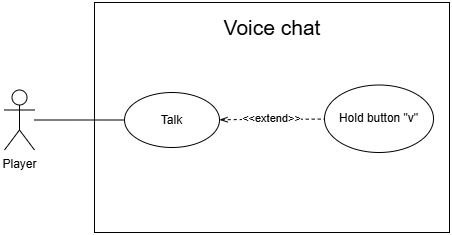
\includegraphics[width=0.75\linewidth]{4.Đặc tả chi tiết các lược đồ/Use-case/images/VoiceChat.png}
    \caption{Use-case mô tả Voice chat}
    \label{fig:placeholder}
\end{figure}


\begin{table}[H]
\centering
\begin{tabular}{|p{4cm}|p{10cm}|}
\hline
\textbf{Use-case name} & Voice chat \\ \hline
\textbf{Actor} & Người chơi \\ \hline
\textbf{Descriptions} & Use-case này sẽ chỉ ra các bước cần thực hiện để có thể sử dụng voice chat được. \\ \hline
\textbf{Pre-conditions} & Phải vào được trong lobby \\ \hline
\textbf{Trigger} & Không có. \\ \hline
\textbf{Post-conditions} & Không có \\ \hline
\textbf{Normal Flow} &
\begin{enumerate}
\item Người chơi nhấn giữ phím ''V''.
\item Người chơi bắt đầu nói chuyện bình thường.
\item Use-case kết thúc sau khi người chơi thả nút ''v''.
\end{enumerate}
\\ \hline
\textbf{Alternative Flow} &
\begin{enumerate}
\item[E1.] Tại bước 1, nếu người chơi đã bật sẵn chế độ "Push-to-talk" trong setting thì không cần bước 1 và đi đến luôn bước 2
\end{enumerate}
\\ \hline
\textbf{Exception Flow} &
Không có
\\ \hline
\end{tabular}
\end{table}
\subsubsection{Text Chat}
Sơ đồ use-case Text chat:
\begin{figure}[H]
    \centering
    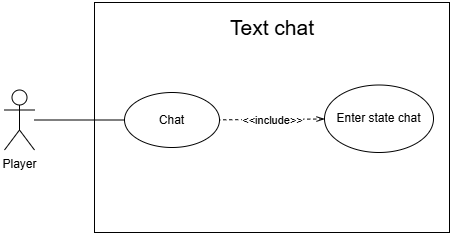
\includegraphics[width=0.75\linewidth]{4.Đặc tả chi tiết các lược đồ/Use-case/images/TextChat.png}
    \caption{Use-case mô tả Text Chat}
    \label{fig:placeholder}
\end{figure}


\begin{table}[H]
\centering
\begin{tabular}{|p{4cm}|p{10cm}|}
\hline
\textbf{Use-case name} & Text chat \\ \hline
\textbf{Actor} & Người chơi \\ \hline
\textbf{Descriptions} & Use-case này sẽ chỉ ra các bước cần thực hiện để có thể sử dụng text chat được. \\ \hline
\textbf{Pre-conditions} & Phải vào được trong lobby \\ \hline
\textbf{Trigger} & Không có. \\ \hline
\textbf{Post-conditions} & Không có \\ \hline
\textbf{Normal Flow} &
\begin{enumerate}
\item Người chơi nhấn phím ''Enter'' để vào chế độ chat.
\item Người chơi bắt đầu ghi các tin nhắn mong muốn.
\item Người chơi nhấn phím ''Enter'' để gửi tin nhắn.
\item Use-case kết thúc sau khi người chơi nhấn phím ''Enter'' để thoát khỏi chế độ chat.
\end{enumerate}
\\ \hline
\textbf{Alternative Flow} &
Không có
\\ \hline
\textbf{Exception Flow} &
Không có
\\ \hline
\end{tabular}
\end{table}


\newpage
% \section{Đặc tả các lược đồ}
% \subsection{Các use-case và các kịch bản}
\subsection{Thiết kế class diagram}

\begin{figure}[H]
    \centering
    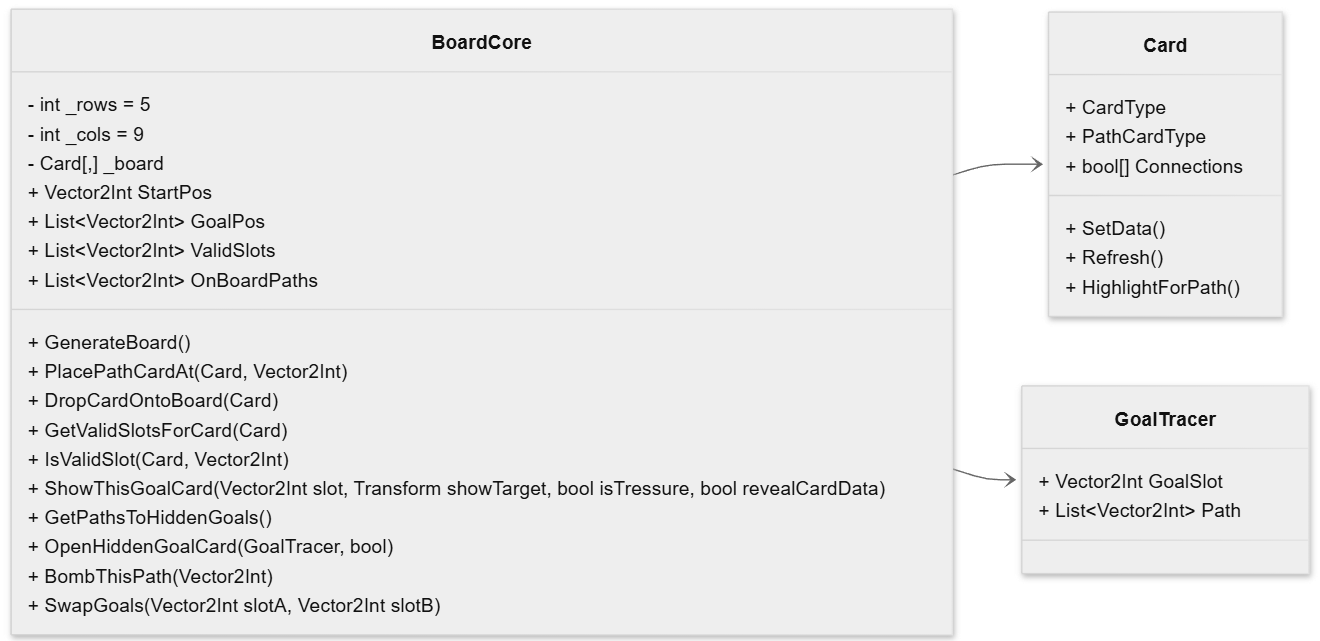
\includegraphics[width=0.9\linewidth]{9.Đặc tả các lược đồ/diagram/board_core.png} 
    \caption{Board Core}
    \label{fig:placeholder}
\end{figure}
\textbf{BoardCore} là thành phần cốt lõi quản lý logic bàn cờ trong trò chơi. Lớp chịu trách nhiệm khởi tạo bàn cờ (GenerateBoard), đặt và kiểm tra vị trí các lá bài đường đi, quản lý các mục tiêu ẩn, cùng các chức năng đặc biệt như phá đường và hoán đổi thẻ dích,... Lớp tương tác chặt chẽ với lớp \textbf{Card} và \textbf{GoalTracer} để xử lý kết nối đường đi và tương tác với thẻ dích.

\begin{figure}[H]
    \centering
    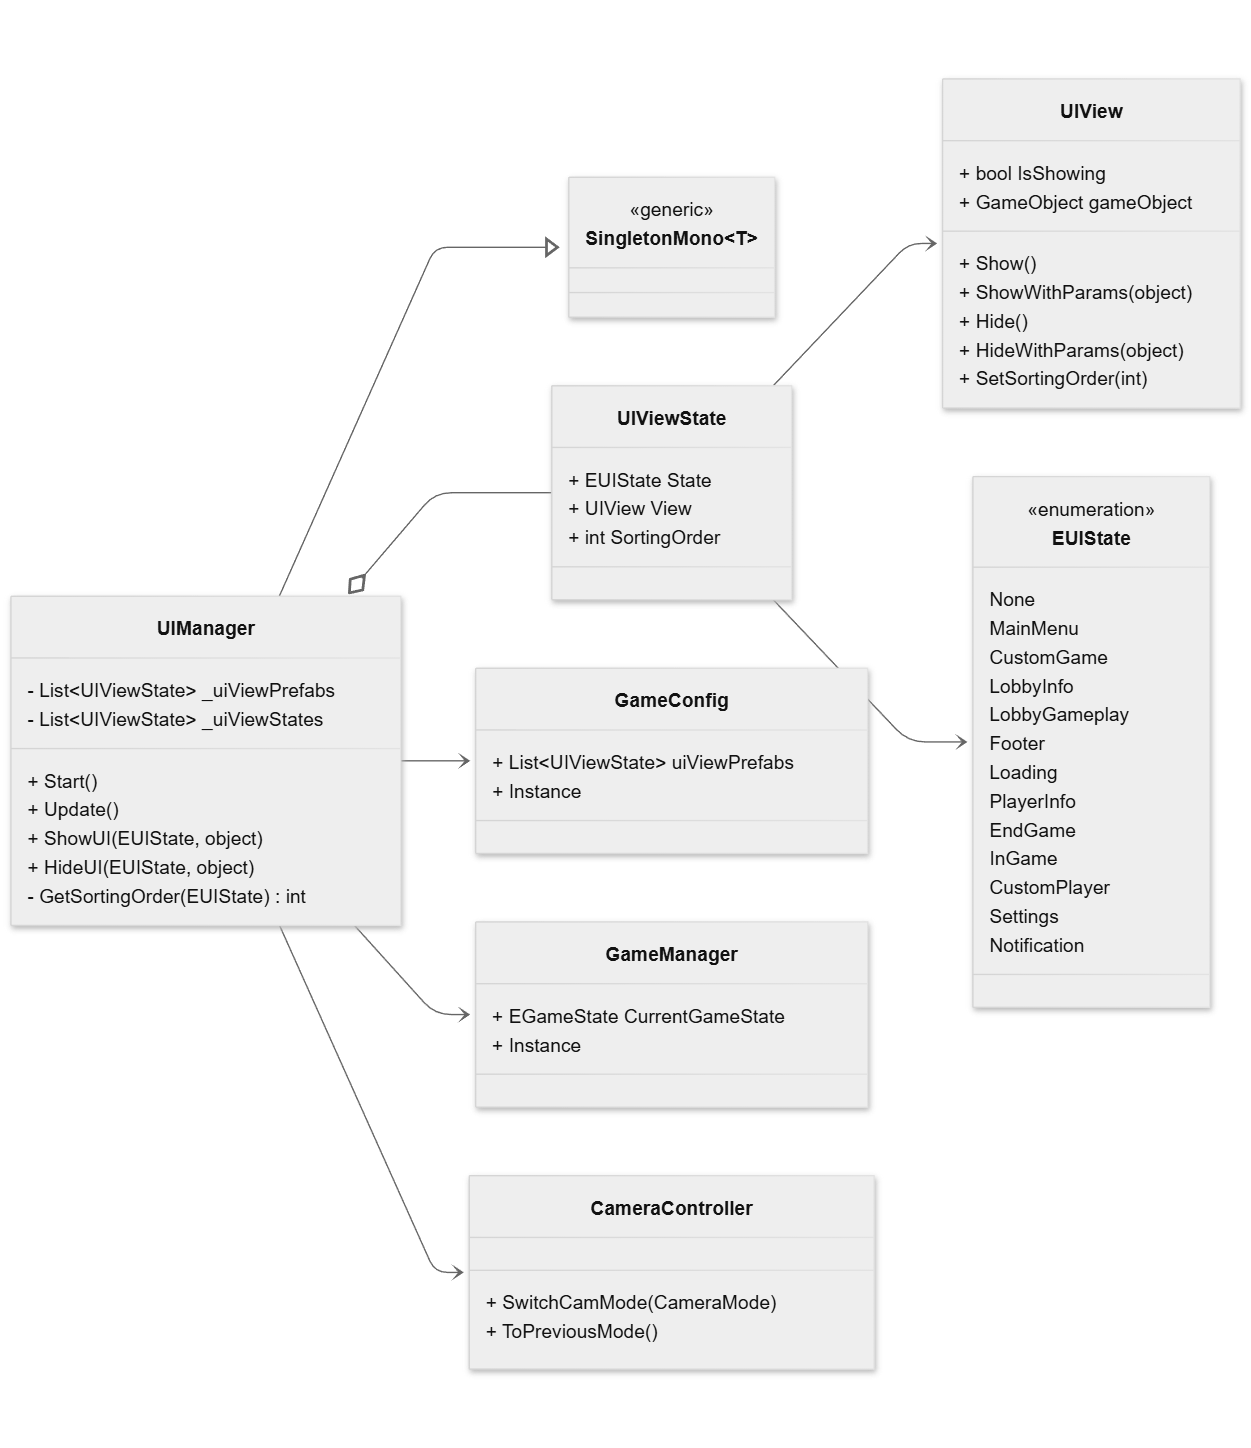
\includegraphics[width=0.9\linewidth]{9.Đặc tả các lược đồ/diagram/UIManager.png}
    \caption{UI Manger}
    \label{fig:placeholder}
\end{figure}
\textbf{UIManager} kế thừa từ \textit{SingletonMono} chịu trách nhiệm quản lý và hiển thị các giao diện người dùng theo trạng thái (EUIState). Lớp sử dụng cơ chế UIViewState và UIView để kiểm soát việc show/hide các giao diện, sắp xếp thứ tự (sorting order).

\begin{figure}[H]
    \centering
    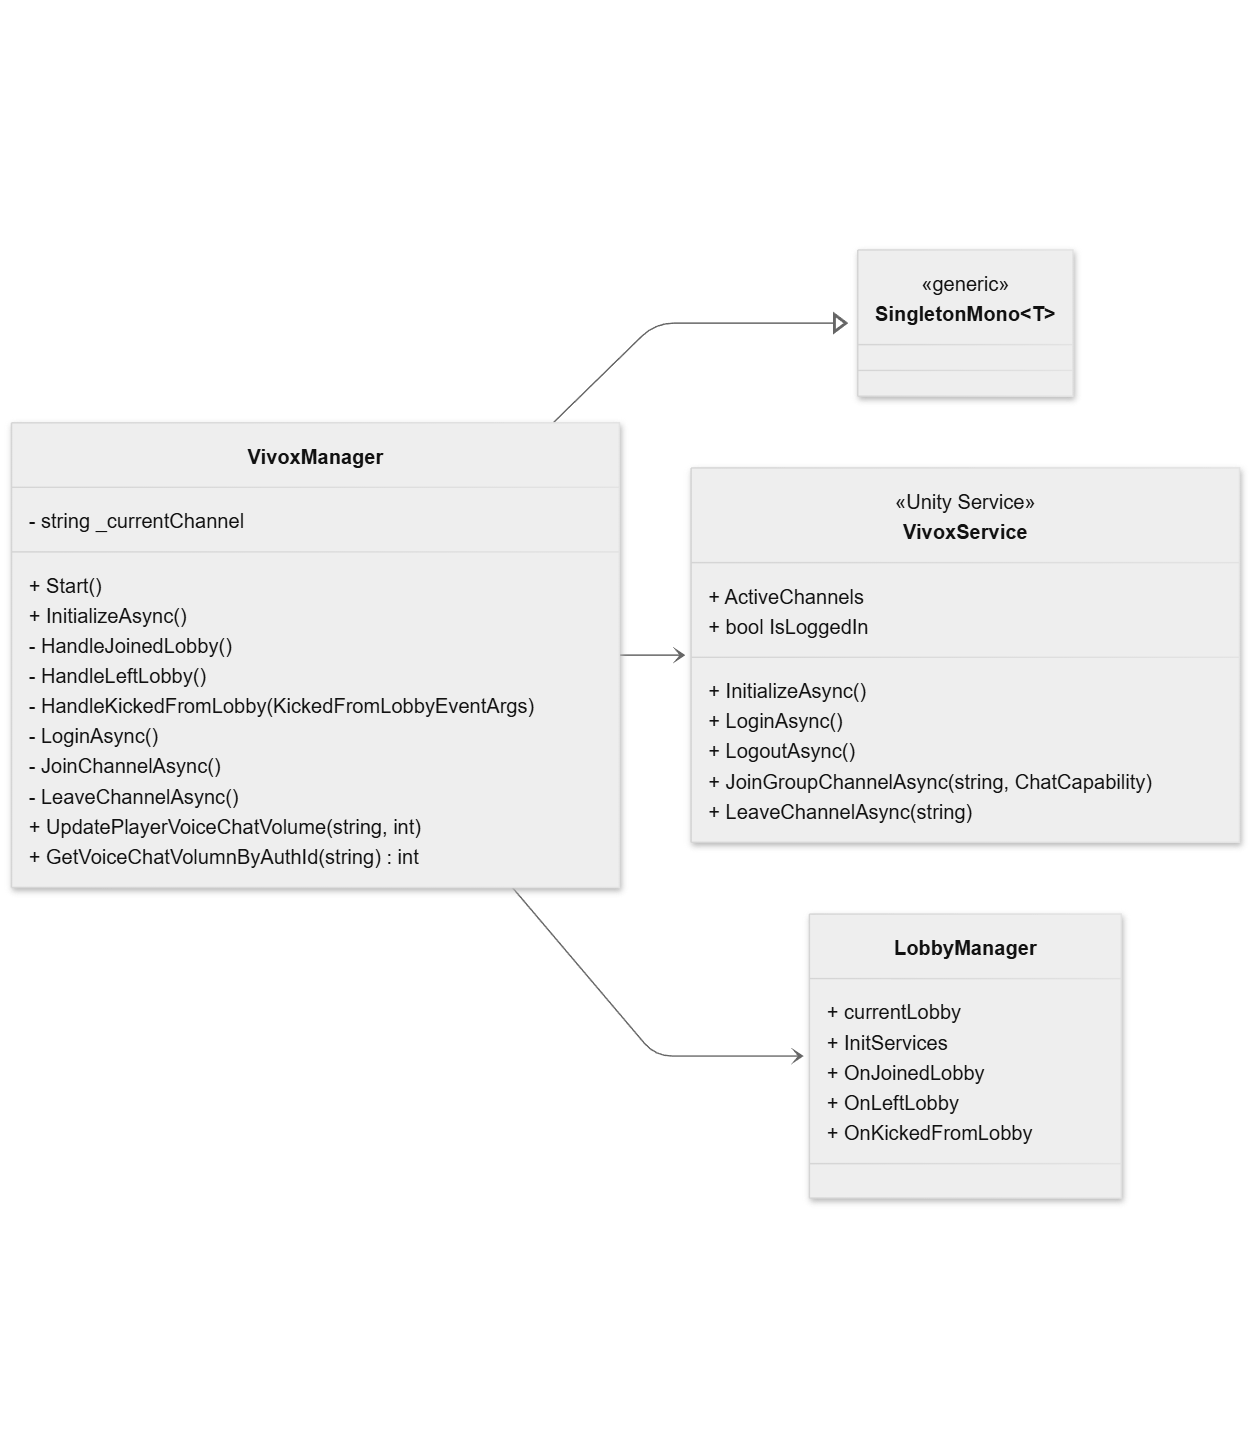
\includegraphics[width=0.9\linewidth]{9.Đặc tả các lược đồ//diagram/vivox_voice_manager.png}
    \caption{Vivox Voice Manager}
    \label{fig:placeholder}
\end{figure}
\textbf{VivoxManager} kế thừa từ \textit{SingletonMono} quản lý hệ thống voice-text chat trong trò chơi. Lớp xử lý việc đăng nhập Vivox, tham gia/rời kênh thoại theo lobby, và điều chỉnh âm lượng giọng nói của từng người chơi.

\noindent
\begin{figure}[H]
    \centering
    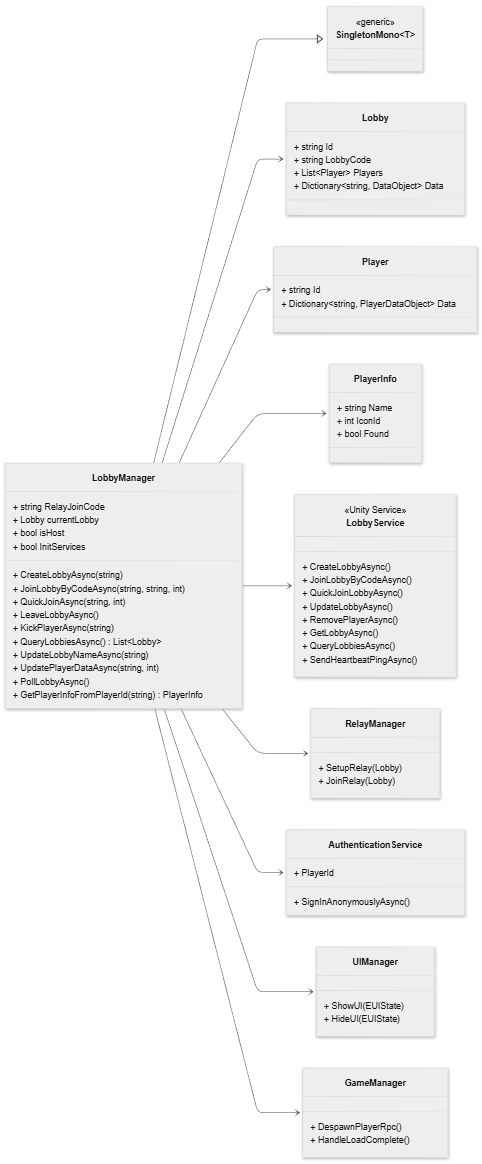
\includegraphics[width=0.5\linewidth]{9.Đặc tả các lược đồ//diagram/lobby_manager.png}
    \caption{Lobby Manager}
    \label{fig:placeholder}
\end{figure}
\textbf{LobbyManager} kế thừa từ \textit{SingletonMono} chịu trách nhiệm quản lý toàn bộ các chức năng liên quan đến lobby. Lớp cung cấp các phương thức bất đồng bộ để tạo lobby, tham gia lobby (quick join hoặc bằng code), cập nhật thông tin lobby, kick người chơi và tích hợp Relay để kết nối mạng. Lớp tương tác chặt chẽ với \textit{LobbyService}, \textbf{RelayManager} và \textit{AuthenticationService} của Unity.

\begin{figure}[H] 
    \centering
    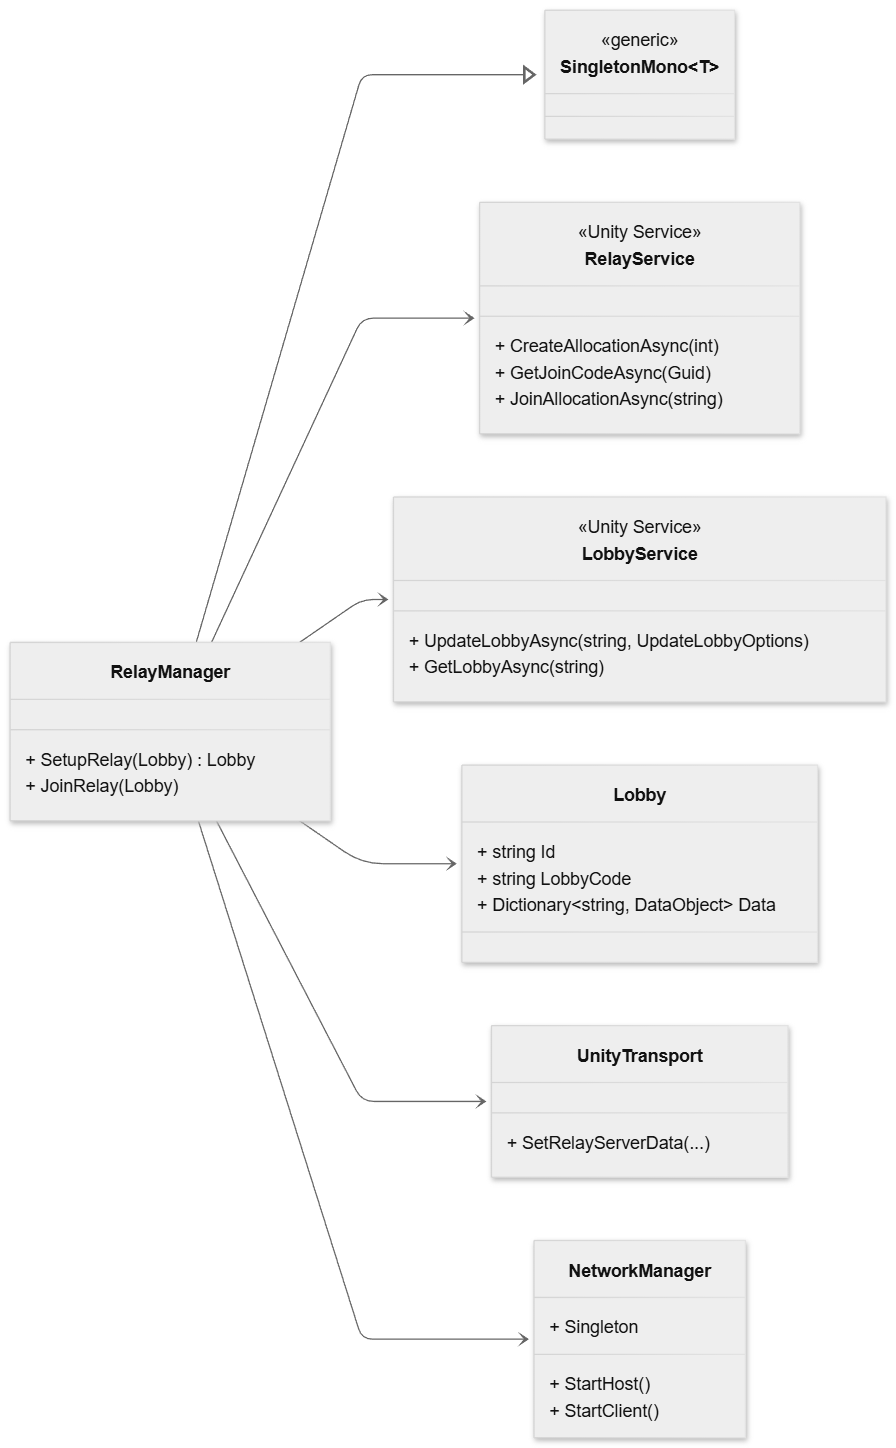
\includegraphics[width=0.6\linewidth]{9.Đặc tả các lược đồ//diagram/relay_manager.png}
    \caption{Relay Manager}
    \label{fig:placeholder}
\end{figure}
\textbf{RelayManager} kế thừa từ \textit{SingletonMono} chịu trách nhiệm thiết lập và quản lý kết nối Relay của Unity để hỗ trợ giao tiếp mạng P2P. Lớp cung cấp các chức năng SetupRelay và JoinRelay, tương tác với \textit{RelayService} và \textit{LobbyService} nhằm tạo allocation và thiết lập server relay cho các phiên chơi.

\begin{figure}[H]
    \centering
    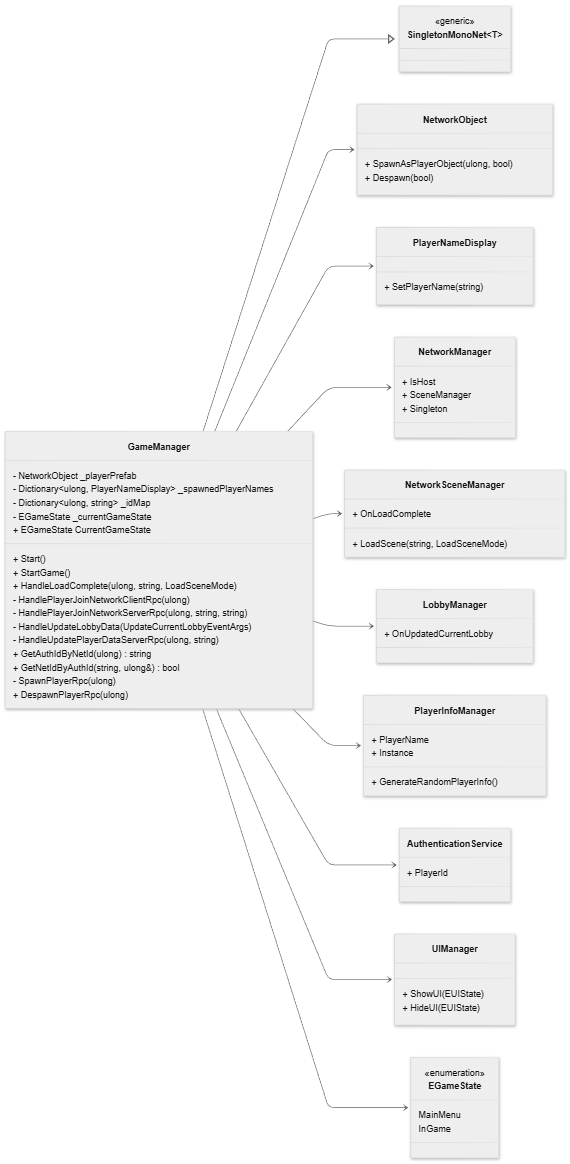
\includegraphics[width=0.5\linewidth]{9.Đặc tả các lược đồ/diagram/game_manager.png}
    \caption{Game Manger}
    \label{fig:placeholder}
\end{figure}
\textbf{GameManager} kế thừa từ \textit{SingletonMonoNet} đóng vai trò trung tâm quản lý trạng thái và vòng đời của trò chơi. Lớp xử lý việc spawn/despawn người chơi, chuyển cảnh, đồng bộ trạng thái lobby và quản lý game state (EGameState). Đây là lớp chính kết nối giữa hệ thống mạng (\textit{NetworkManager}), lobby và giao diện người chơi.
\begin{figure}[H]
    \centering
    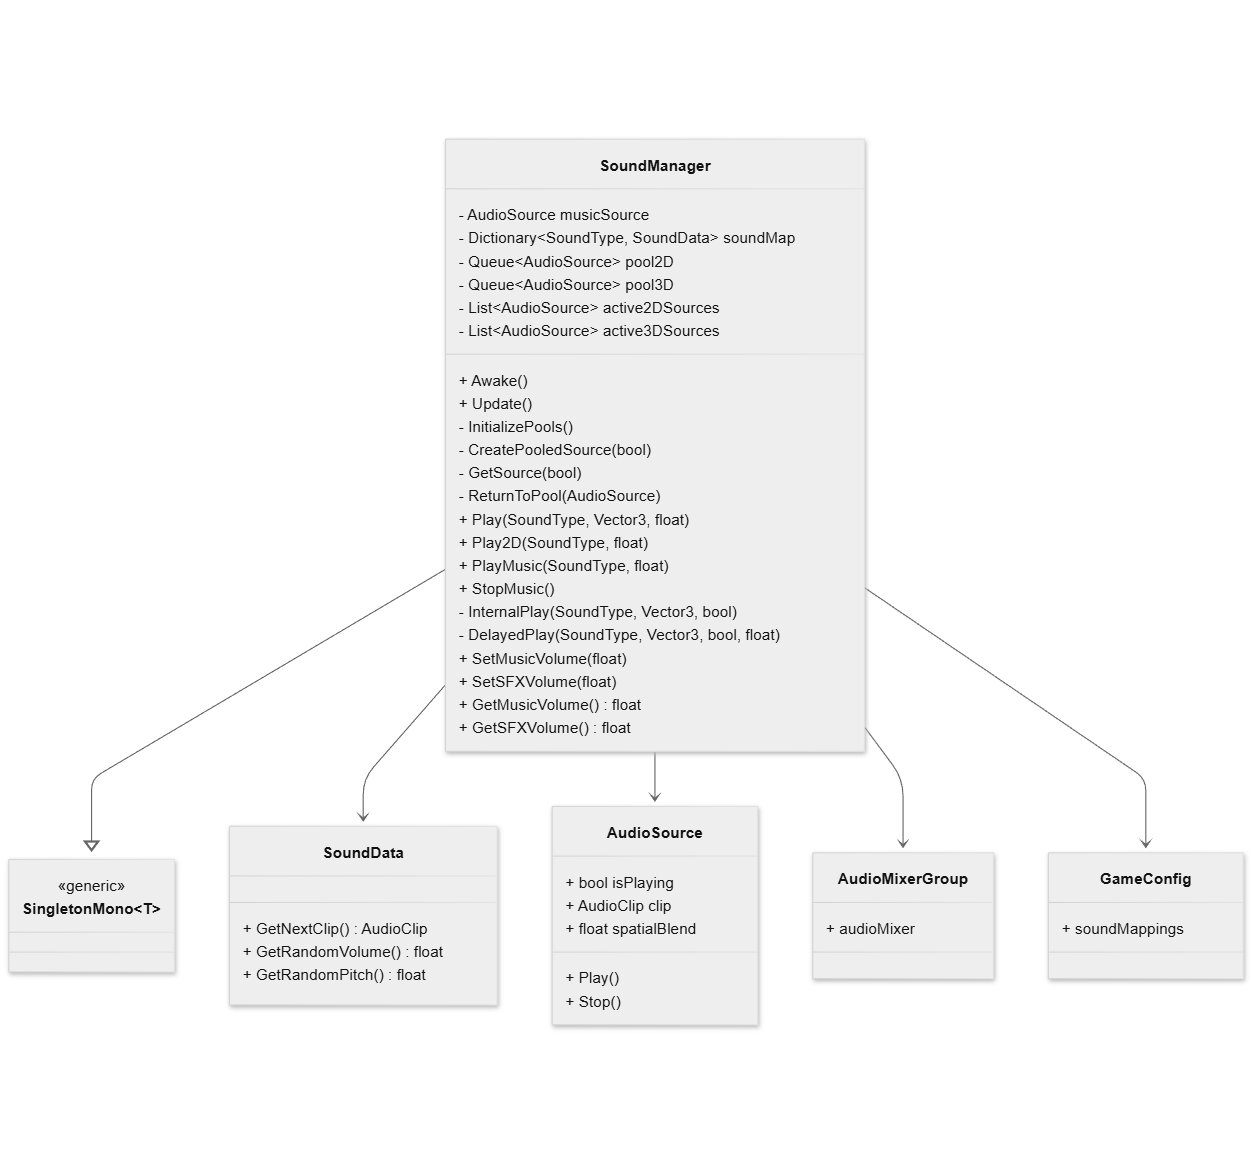
\includegraphics[width=0.9\linewidth]{9.Đặc tả các lược đồ/diagram/sound_manager.png}
    \caption{Sound Manger}
    \label{fig:placeholder}
\end{figure}
\textbf{SoundManager} kế thừa từ \textit{SingletonMono} quản lý hệ thống âm thanh toàn cục của trò chơi. Lớp hỗ trợ phát nhạc nền, hiệu ứng âm thanh 2D/3D với hệ thống object pooling, điều chỉnh âm lượng và quản lý các AudioSource một cách hiệu quả.

\newpage
% \section{Đặc tả các lược đồ}
% \subsection{Các use-case và các kịch bản}
\subsection{Thiết kế class diagram}

\begin{figure}[H]
    \centering
    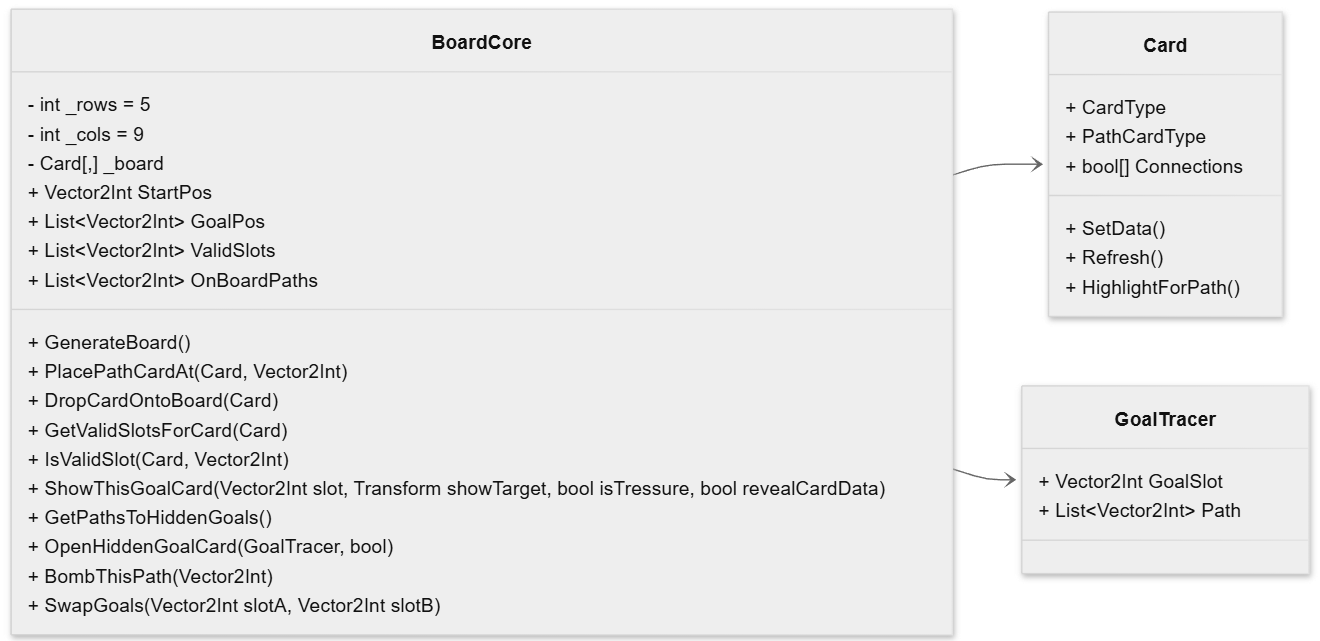
\includegraphics[width=0.9\linewidth]{9.Đặc tả các lược đồ/diagram/board_core.png} 
    \caption{Board Core}
    \label{fig:placeholder}
\end{figure}
\textbf{BoardCore} là thành phần cốt lõi quản lý logic bàn cờ trong trò chơi. Lớp chịu trách nhiệm khởi tạo bàn cờ (GenerateBoard), đặt và kiểm tra vị trí các lá bài đường đi, quản lý các mục tiêu ẩn, cùng các chức năng đặc biệt như phá đường và hoán đổi thẻ dích,... Lớp tương tác chặt chẽ với lớp \textbf{Card} và \textbf{GoalTracer} để xử lý kết nối đường đi và tương tác với thẻ dích.

\begin{figure}[H]
    \centering
    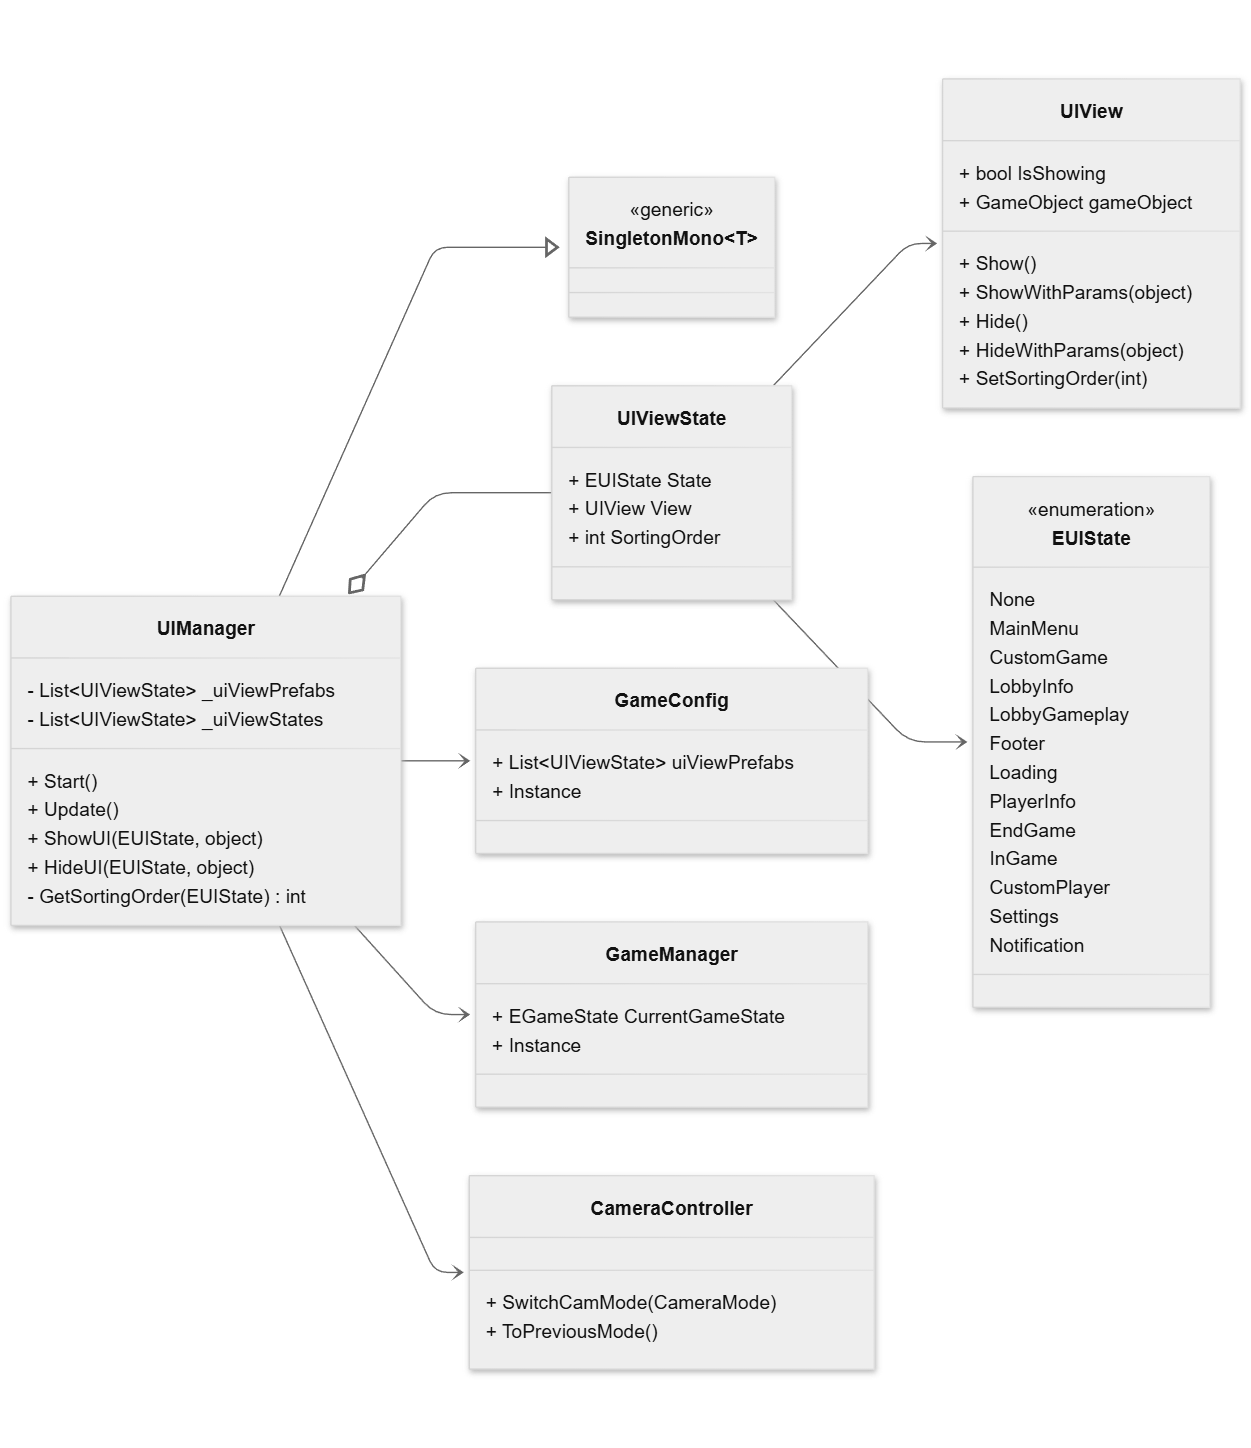
\includegraphics[width=0.9\linewidth]{9.Đặc tả các lược đồ/diagram/UIManager.png}
    \caption{UI Manger}
    \label{fig:placeholder}
\end{figure}
\textbf{UIManager} kế thừa từ \textit{SingletonMono} chịu trách nhiệm quản lý và hiển thị các giao diện người dùng theo trạng thái (EUIState). Lớp sử dụng cơ chế UIViewState và UIView để kiểm soát việc show/hide các giao diện, sắp xếp thứ tự (sorting order).

\begin{figure}[H]
    \centering
    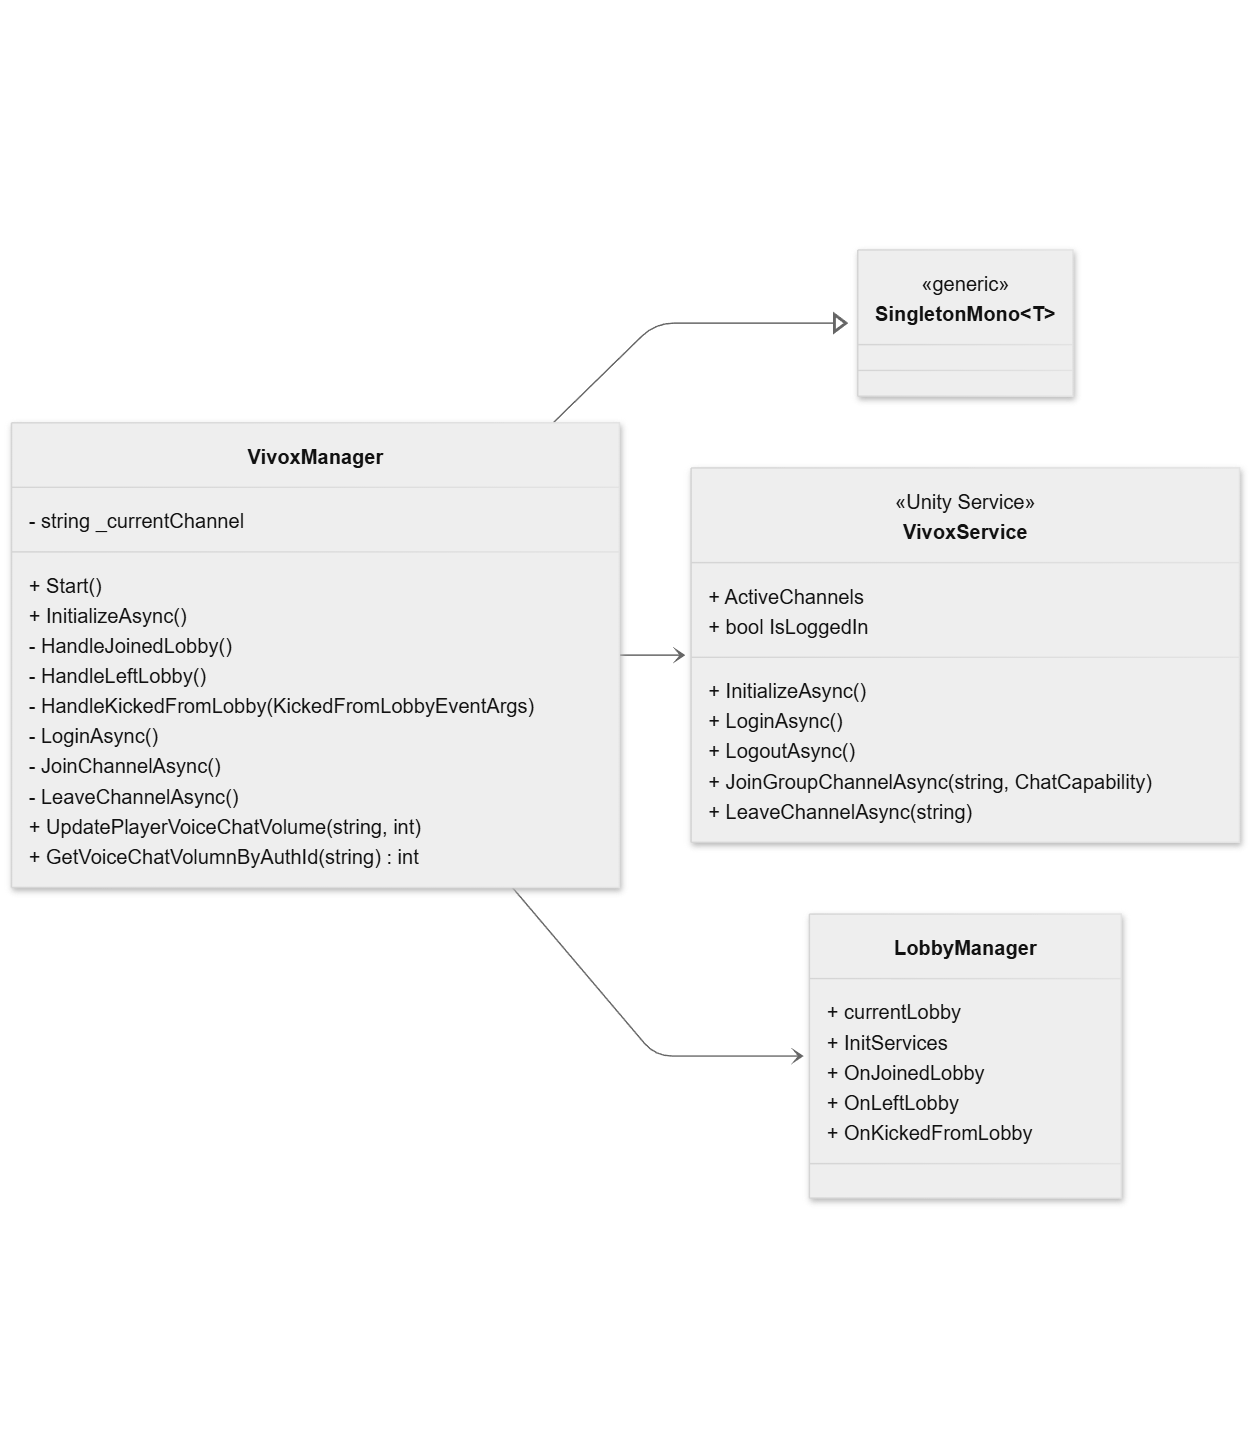
\includegraphics[width=0.9\linewidth]{9.Đặc tả các lược đồ//diagram/vivox_voice_manager.png}
    \caption{Vivox Voice Manager}
    \label{fig:placeholder}
\end{figure}
\textbf{VivoxManager} kế thừa từ \textit{SingletonMono} quản lý hệ thống voice-text chat trong trò chơi. Lớp xử lý việc đăng nhập Vivox, tham gia/rời kênh thoại theo lobby, và điều chỉnh âm lượng giọng nói của từng người chơi.

\noindent
\begin{figure}[H]
    \centering
    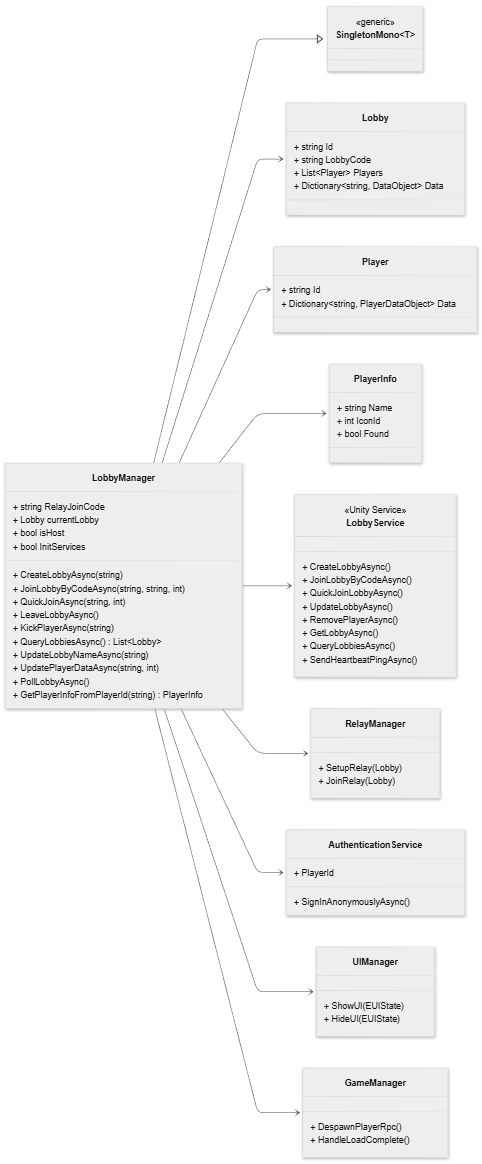
\includegraphics[width=0.5\linewidth]{9.Đặc tả các lược đồ//diagram/lobby_manager.png}
    \caption{Lobby Manager}
    \label{fig:placeholder}
\end{figure}
\textbf{LobbyManager} kế thừa từ \textit{SingletonMono} chịu trách nhiệm quản lý toàn bộ các chức năng liên quan đến lobby. Lớp cung cấp các phương thức bất đồng bộ để tạo lobby, tham gia lobby (quick join hoặc bằng code), cập nhật thông tin lobby, kick người chơi và tích hợp Relay để kết nối mạng. Lớp tương tác chặt chẽ với \textit{LobbyService}, \textbf{RelayManager} và \textit{AuthenticationService} của Unity.

\begin{figure}[H] 
    \centering
    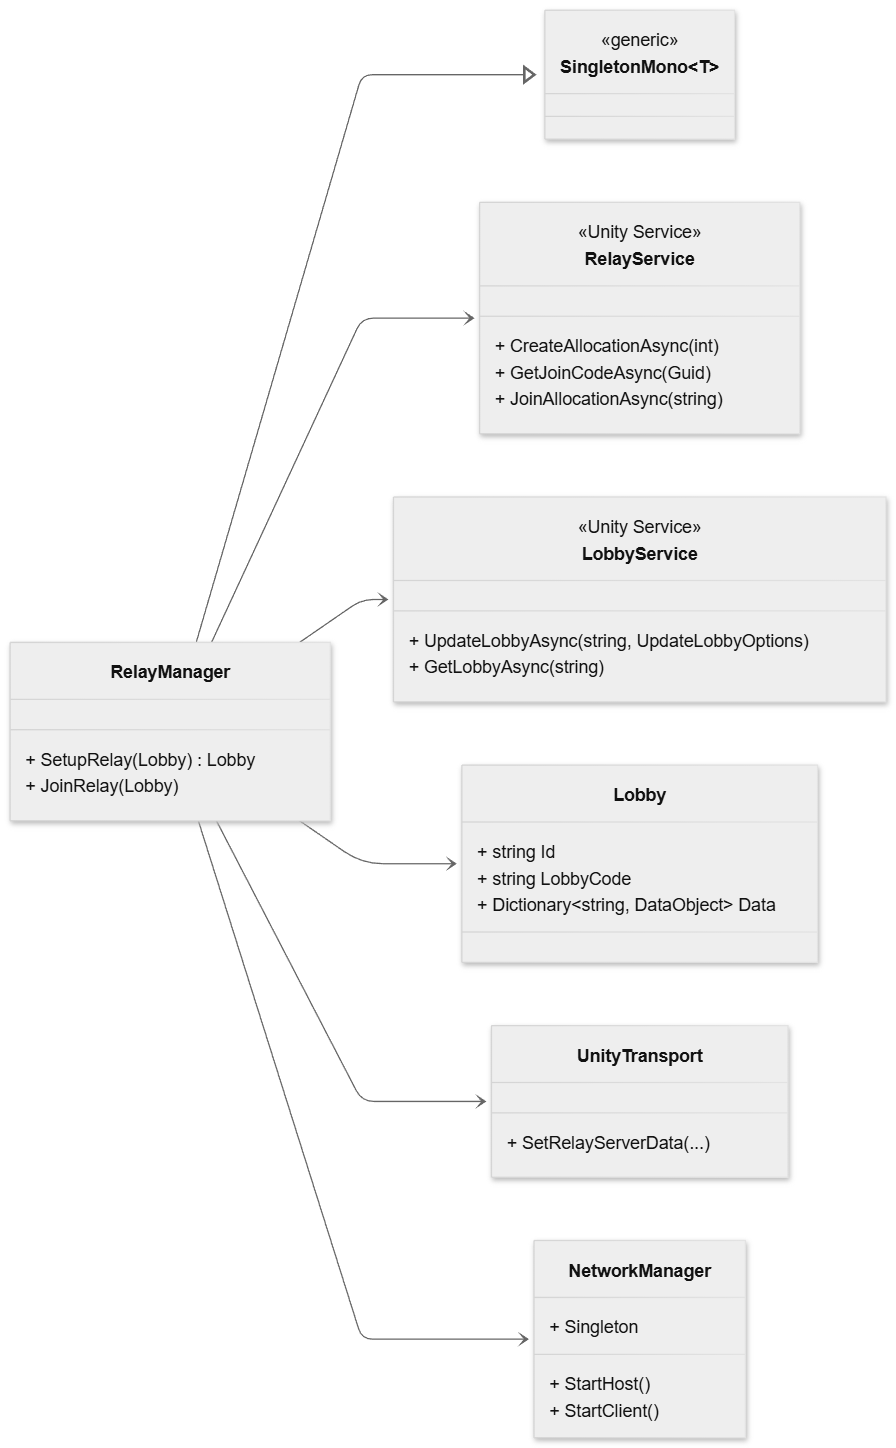
\includegraphics[width=0.6\linewidth]{9.Đặc tả các lược đồ//diagram/relay_manager.png}
    \caption{Relay Manager}
    \label{fig:placeholder}
\end{figure}
\textbf{RelayManager} kế thừa từ \textit{SingletonMono} chịu trách nhiệm thiết lập và quản lý kết nối Relay của Unity để hỗ trợ giao tiếp mạng P2P. Lớp cung cấp các chức năng SetupRelay và JoinRelay, tương tác với \textit{RelayService} và \textit{LobbyService} nhằm tạo allocation và thiết lập server relay cho các phiên chơi.

\begin{figure}[H]
    \centering
    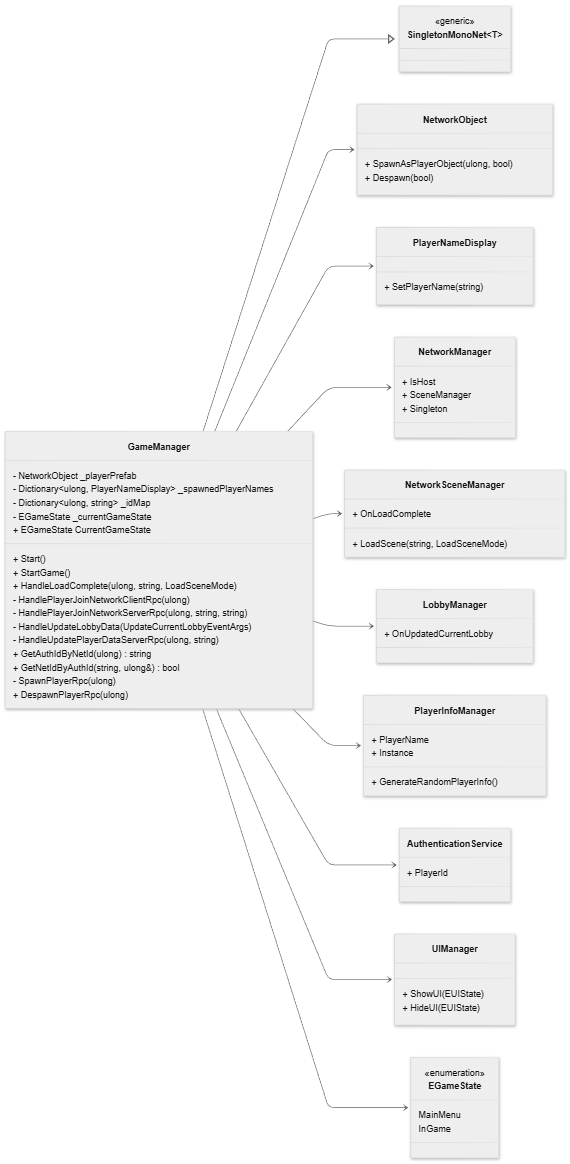
\includegraphics[width=0.5\linewidth]{9.Đặc tả các lược đồ/diagram/game_manager.png}
    \caption{Game Manger}
    \label{fig:placeholder}
\end{figure}
\textbf{GameManager} kế thừa từ \textit{SingletonMonoNet} đóng vai trò trung tâm quản lý trạng thái và vòng đời của trò chơi. Lớp xử lý việc spawn/despawn người chơi, chuyển cảnh, đồng bộ trạng thái lobby và quản lý game state (EGameState). Đây là lớp chính kết nối giữa hệ thống mạng (\textit{NetworkManager}), lobby và giao diện người chơi.
\begin{figure}[H]
    \centering
    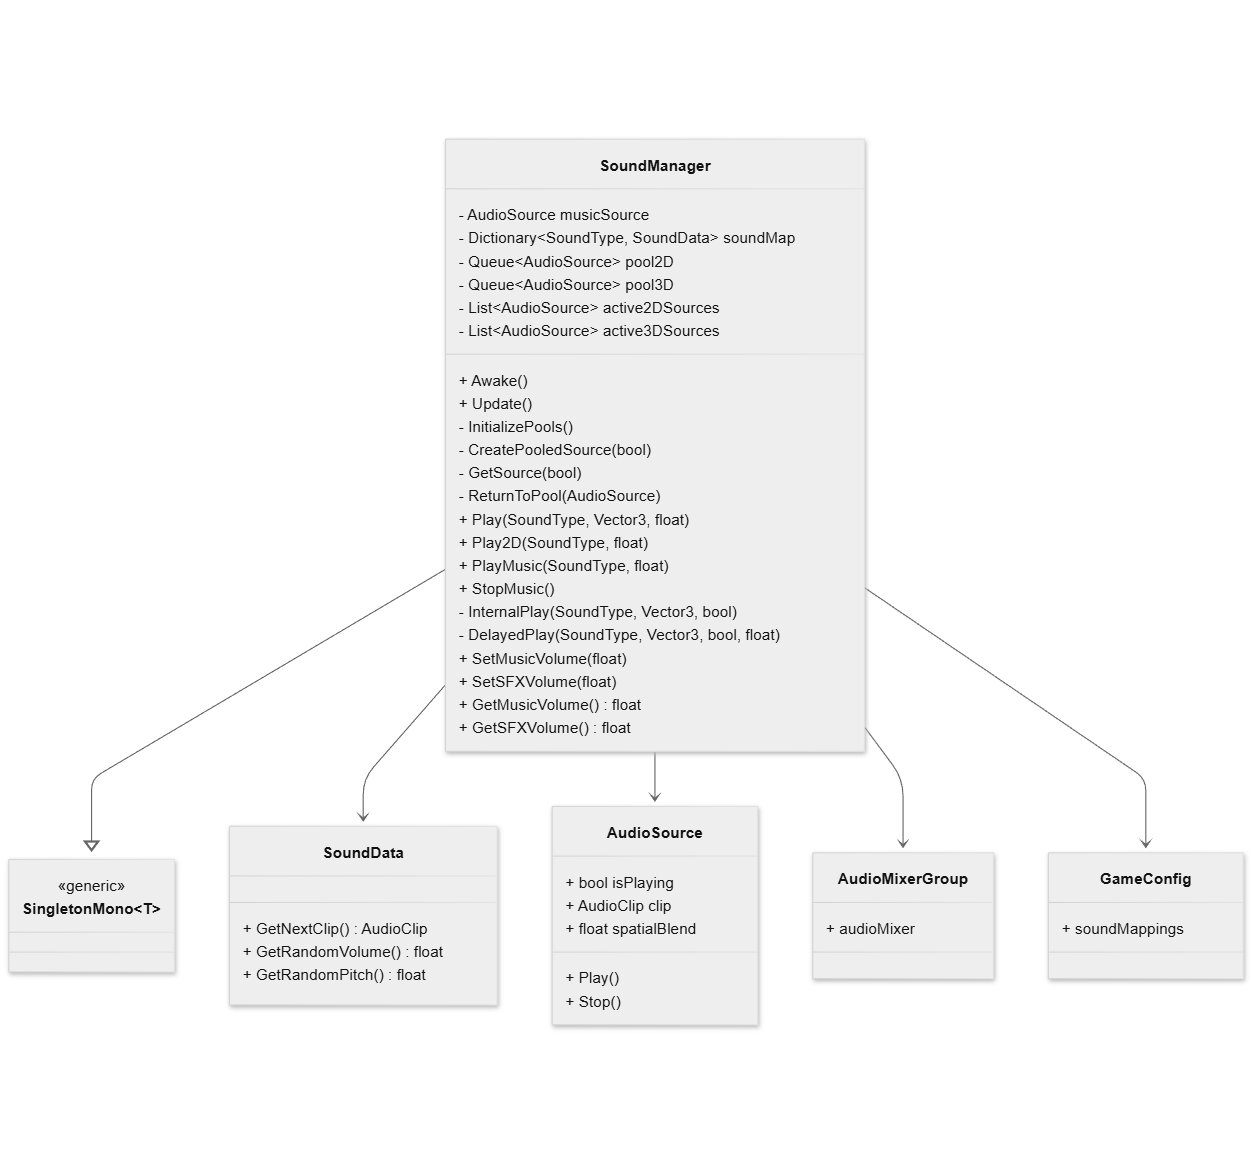
\includegraphics[width=0.9\linewidth]{9.Đặc tả các lược đồ/diagram/sound_manager.png}
    \caption{Sound Manger}
    \label{fig:placeholder}
\end{figure}
\textbf{SoundManager} kế thừa từ \textit{SingletonMono} quản lý hệ thống âm thanh toàn cục của trò chơi. Lớp hỗ trợ phát nhạc nền, hiệu ứng âm thanh 2D/3D với hệ thống object pooling, điều chỉnh âm lượng và quản lý các AudioSource một cách hiệu quả.
\section{Phân tích \& Thiết kế hệ thống}
\subsection{Các Stakeholder và User story}
\subsubsection{Stakeholder}
Hệ thống bao gồm stakeholder là người chơi, chính là những người tham gia trò chơi, có thể là một hoặc nhiều người tùy theo số lượng người vào cùng 1 phòng trong trò chơi.
\subsubsection{User story của người chơi}
Ta có thể có được các user story đối với các chức năng, trường hợp trong trò chơi. Cụ thể về các user story:

\begin{itemize}
    \item  Đối với user story về các luồng thực thi ở trang chủ của trò chơi, là người chơi, tôi có thể:
        \begin{itemize}
            \item Chọn tạo phòng hoặc tham gia phòng của người chơi khác.
            \item Điều chỉnh các thông số cấu hình của trò chơi khi truy cập vào cài đặt.
            \item Xem thông tin cá nhân của người chơi.
            \item Xem thông tin về nhà phát triển của trò chơi.
        \end{itemize}
    \item Đối với user story về các luồng thực thi khi đã vào phòng của trò chơi, là người chơi, tôi có thể:
        \begin{itemize}
            \item Xem thông tin phòng chơi.
            \item Sử dụng các nhạc cụ có trong phòng.
            \item Thay đổi trang phục.
            \item Ngồi vào bàn và bắt đầu chơi (nếu đã đủ số lượng người chơi tối thiểu).
            \item Nếu là chủ phòng thì có thể kick người chơi khác khỏi phòng của mình.
        \end{itemize}
    \item Đối với user story về gameplay của trò chơi, là người chơi, tôi có thể:
        \begin{itemize}
            \item Xem hướng dẫn về trò chơi như luật, cách chơi về board game.
            \item Kết thúc màn chơi hiện tại. Sau khi kết thúc, tôi có thể chọn một trong các lựa chọn: bắt đầu lại hoặc rời khỏi ghế và làm những thứ khác.
        \end{itemize}
    \item Đối với user story về các tùy chỉnh cấu hình khi truy cập vào cài đặt trong trò chơi, là người chơi, tôi có thể:
        \begin{itemize}
            \item Điều chỉnh các thông số chung của trò chơi như âm nhạc, âm thanh.
        \end{itemize}
\end{itemize}
\subsection{Kiến trúc tổng thể}
Dự án được xây dựng bằng Unity, sử dụng công cụ NGO (Network for GameObjects) cho phần Networking (multiplayer) và thiết kế dựa trên mô hình Client-Host ở giai đoạn này (giai đoạn 1).
\subsubsection{Kiến trúc dự án Unity}
Một dự án được xây dựng trên kiến trúc gồm có 3 lớp chính:
\begin{enumerate}[$\bullet$]
    \item Lớp Asset: chứa các model 3D, texture, material, file nhạc, âm thanh, script, prefab,...
    \item Lớp Runtime: gồm các Scene và toàn bộ GameObject cùng với các component của nó khi game chạy.
    \item Lớp Engine System: gồm hệ thống vật lý, âm thanh, render, input, event loop của engine Unity.
\end{enumerate}

Các lớp được hoạt động theo mô hình pipeline của Unity. Trong quá trình phát triển, lập trình viên tương tác chính với các GameObject, Component và các tài nguyên của game (lớp Asset). Sau đây nhóm sẽ nêu các đặc điểm chính của các thành phần quan trọng mà nhà phát triển sẽ làm việc trong dự án Unity:
\begin{enumerate}[$\bullet$]
    \item \textbf{GameObject}: 
    \begin{enumerate}[-]
        \item Đây là thực thể cơ bản nhất trong Scene, nó hoạt động như một container trống chứa các Component.
        \item Đại diện cho các đối tượng trong game như: nhân vật, camera, UI, map,...
        \item Không chứ bất kì logic nào, tất cả logic, hành vi do các component xử lý.
        \item Tổ chức cấu trúc dạng cha-con (hierachy) trực quan.
    \end{enumerate}
    \begin{figure}[!h]
        \centering
        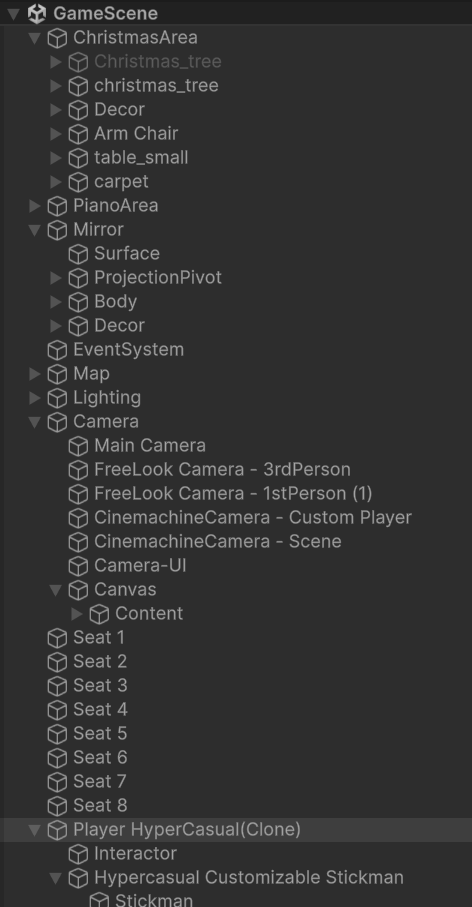
\includegraphics[width=3cm]{5.Thiết kế/images/game-object.png}
        \caption{Cấu trúc mẫu của các GameObject trong Scene (GameScene)}
        \label{fig:game-object}
    \end{figure}
    \newpage
    \item \textbf{Component}:
    \begin{enumerate}[-]
        \item Là nơi định nghĩa các hành vi và dữ liệu của GameObject. Ví dụ như Component Transform là một component bắt buộc có của mọi GameObject, nó giúp biểu diễn vị trí (tọa độ, hướng) và scale của đối tượng.
        \item Gồm các Component được viết sẵn của Unity và các script do lập trình tự viết. 
        \item Tính tái sử dụng cao, dễ mở rộng.
    \end{enumerate}
    \begin{figure}[!h]
        \centering
        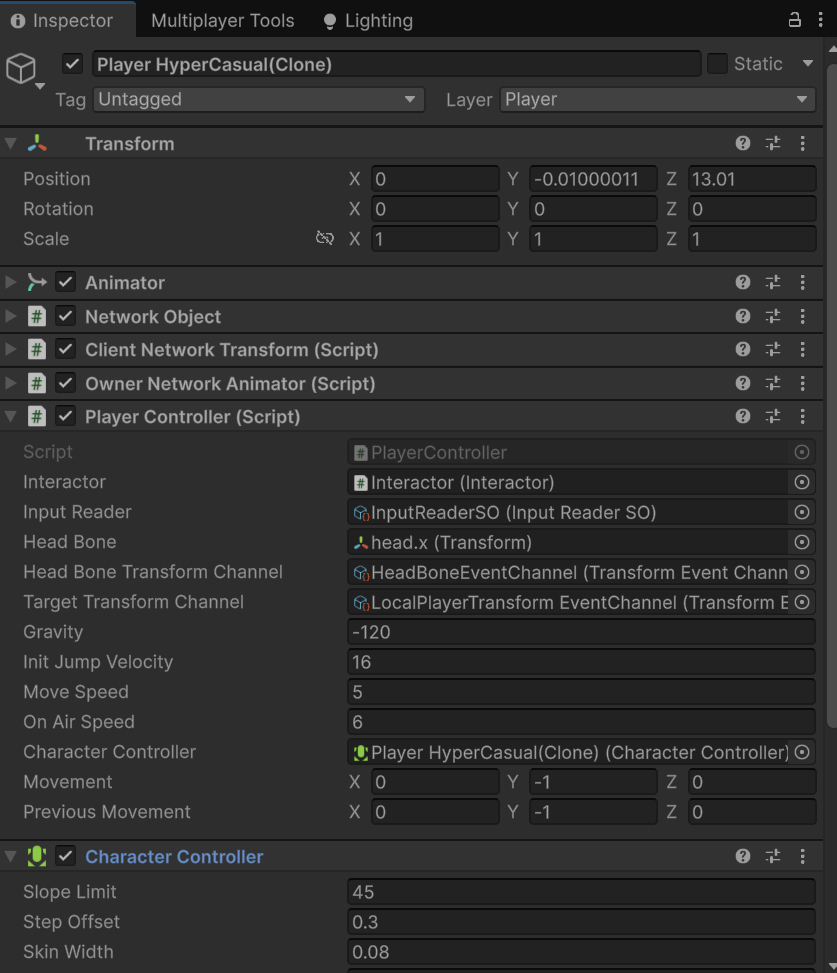
\includegraphics[width=8cm]{5.Thiết kế/images/component.png}
        \caption{Cấu trúc mẫu của các Component trong GameObject (Player)}
        \label{fig:component}
    \end{figure}
    \item \textbf{MonoBehaviour}:
    \begin{enumerate}[-]
        \item Là một class nền tảng của Unity Engine, cung cấp các callback trong lifecycle của Unity:
        \begin{enumerate}[+]
            \item Awake(): khởi tạo dữ liệu của class, chạy khi object được load vào Scene.
            \item Start(): chạy duy nhất 1 lần ngay trước frame đầu tiên sau khi object được kích hoạt.
            \item Update(): chạy mỗi frame khi được kích hoạt.
            \item FixUpdate(): tương tự Update nhưng FPS được giữ cố định, thường dùng cho các logic vật lý.
            \item LateUpdate(): chạy ngay sau Update chạy xong.
            \item OnEnable()/OnDisable(): chạy khi đối tượng được bật/tắt.
            \item OnDestroy(): Chạy khi object bị xóa khỏi Scene, dùng để dọn dẹp tài nguyên.
        \end{enumerate}
        \item Hỗ trợ liên kết dữ liệu giữa các component với hệ thống của Unity, hỗ trợ lập trình event-driven.
    \end{enumerate}
    \newpage
    \item \textbf{ScriptableObject}:
    \begin{enumerate}[-]
        \item Là một asset chứa dữ liệu, độc lập với scene và lifetime của Unity.
        \item Thường dùng lưu trữ dữ liệu tĩnh, có thể tái sử dụng cho nhiều đối tượng như Stats nhân vật, Skill data, Game Config...
        \item Phù hợp cho mô hình Data-Oriented.
    \end{enumerate}
    \begin{figure}[!h]
        \centering
        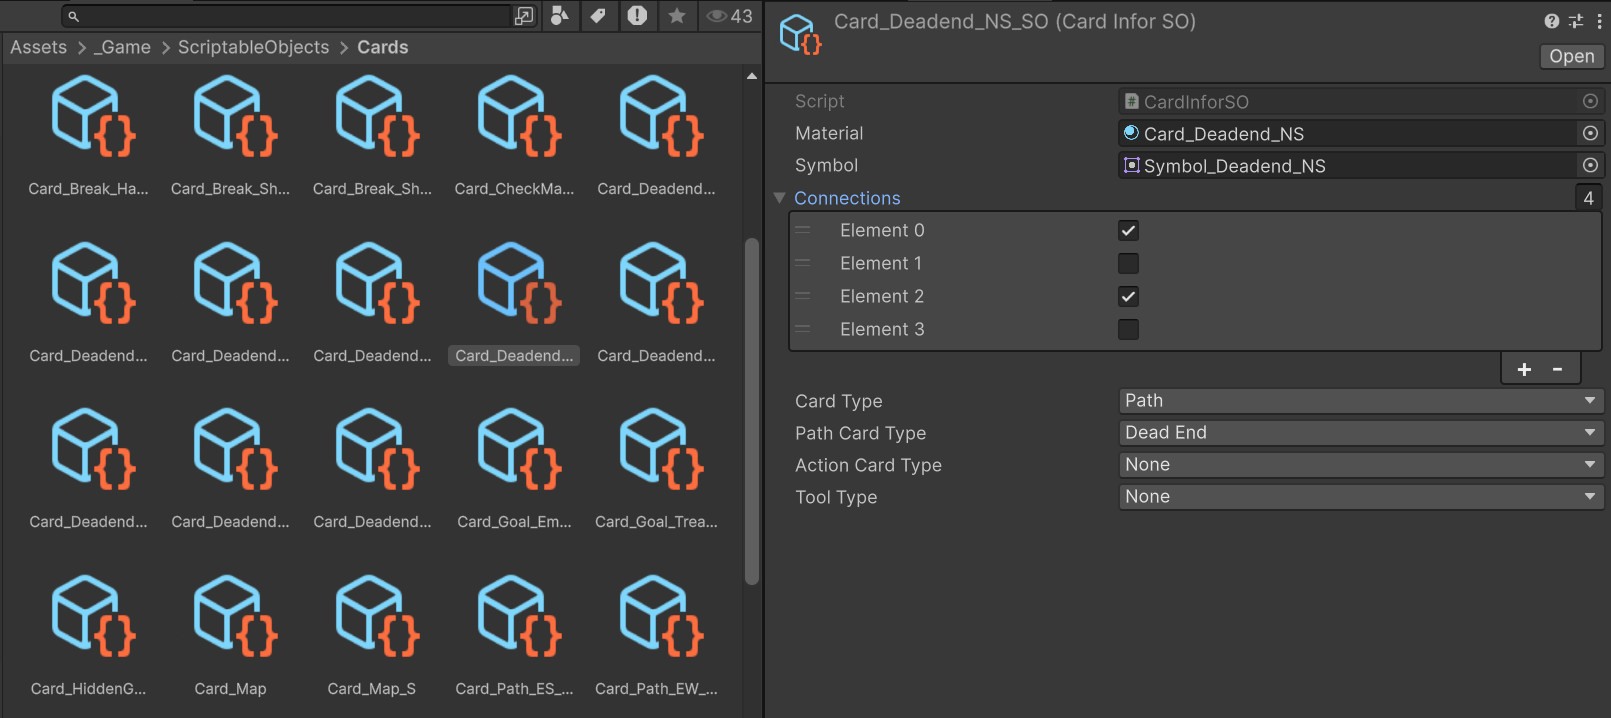
\includegraphics[width=10cm]{5.Thiết kế/images/scriptable-object.png}
        \caption{Các scriptable object sử dụng để lưu dữ liệu Card trong game}
        \label{fig:scriptable-object}
    \end{figure}
    \newpage
    \item \textbf{Prefab}:
    \begin{enumerate}[-]
        \item Là một asset lưu trữ toàn bộ thông tin của một GameObject.
        \item Dùng để tái sử dụng các đối tượng trong game như nhân vật, card ...
        \item Có cơ chế Prefab Variant giúp tạo các Prefab con kế thừa Prefab gốc (Prefab cha thay đổi thì Prefab con cũng thay đổi theo).
    \end{enumerate}
    \begin{figure}[!h]
        \centering
        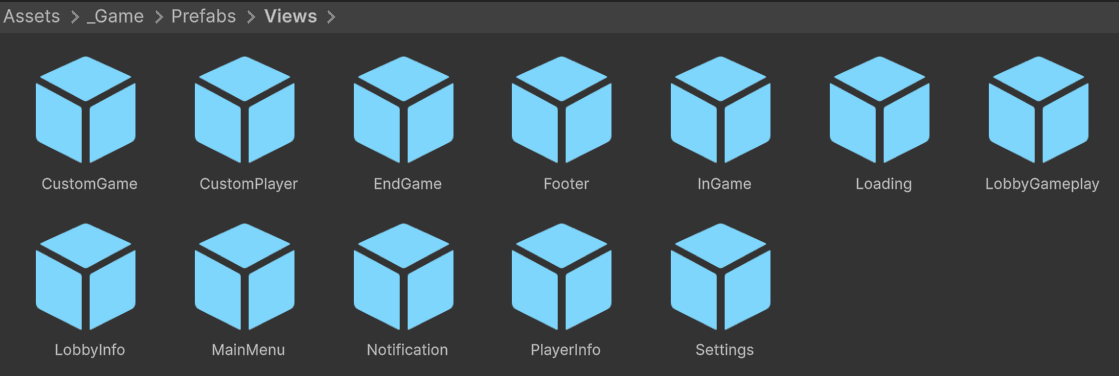
\includegraphics[width=10cm]{5.Thiết kế/images/prefab.png}
        \caption{Các prefab lưu trữ GameObject của UI các screen trong game}
        \label{fig:prefab}
    \end{figure}
    \item \textbf{Scene}:
    \begin{enumerate}[-]
        \item Là không gian chứa tất cả các GameObject.
        \item Thường được chia ra theo module để dễ quản lý: Boot Scene, Gameplay...
        \item Có thể mở nhiều scene cùng lúc (thường dùng cho tách riêng scene UI và scene gameplay).
    \end{enumerate}
   
\end{enumerate}
\subsubsection{Kiến trúc NGO}
NGO là công cụ hỗ trợ xây dụng game multiplayer dựa theo mô hình GameObject do Unity phát triển. NGO có mục tiêu chính là đơn giản hóa các đồng bộ trạng thái, xử lý RPC (remote procedure call), quản lý các kết nối người dùng trong mạng, đồng thời hỗ trợ các kiến trúc mạng khác nhau như client-host và client-server authoritative,

Trong NGO, vòng đời mạng tổng quan như sau:
\begin{enumerate}[+]
    \item Khởi tạo \textbf{NetworkManager}.
    \item Chọn chế độ chạy: Host/Client/Server.
    \item Server khởi tạo danh sách các kết nối.
    \item Server tạo các NetworkObject và thông báo tới Client.
    \item Client tạo bản sao và đồng bộ các trạng thái.
    \item Vòng lặp cập nhật (network tick), xử lý RPC.
    \item Dọn dẹp khi kết thúc: hủy các NetworkObject và hủy các kết nối mạng.
\end{enumerate}

Sau đây, nhóm sẽ giới thiệu các thành phần chính được sử dụng trong một dự án dùng NGO:
\begin{enumerate}[$\bullet$]
    \item \textbf{NetworkManager}:
    \begin{enumerate}[-]
        \item Là thành phần (Component) điều khiển chính của hệ thống mạng, quản lý đồng thời nhiều chức năng:
        \begin{enumerate}[+]
            \item Khởi tạo server, host hoặc client.
            \item Điều khiển tầng vận chuyển (Unity Transport/Custom Transport)
            \item Kiểm soát cập nhật mạng (tick mạng).
            \item Quản lý lifecycle của các NetworkObject trong mạng (tạo/hủy)
            \item Lưu trữ trạng thái, thông tin của các đối tượng kết nối trong mạng (client, server).
        \end{enumerate}
        \item Giao thức mặc định sử dụng là Unity Transport (UTP) hỗ trợ UDP tin cậy, QoS, kết hợp với Relay thông qua Unity Service, 
    \end{enumerate}   
    \item \textbf{NetworkObject}:
    \begin{enumerate}[-]
        \item Là Component bắt buộc cho bất ký GameObject nào muốn tồn tại trong mạng multiplayer, có vai trò quan trọng:
        \begin{enumerate}[+]
            \item Cung cấp mã định danh duy nhất (NetworkInstanceId) giữa tất cả các client.
            \item Quy định ai là chủ sở hữu (owner) của object.
        \end{enumerate}
        \item Chịu sử quản lý của NetworkManager khi tạo/hủy. Các thao tác server thực hiện để tạo (spawn) một NetworkGameobject:
        \begin{enumerate}[+]
            \item Server tạo instance trong scene.
            \item Object sẽ được cấp mã định danh.
            \item Server gửi thông báo đến tất cả các client.
            \item Client tạo bản sao tương ứng với NetworkObject được tạo trên server,
        \end{enumerate}
    \end{enumerate}
    \item \textbf{NetworkBehaviour}:
    \begin{enumerate}[-]
        \item Là một Component kế thừa từ MonoBehaviour và có thêm thêm các tính năng về mạng:
        \begin{enumerate}[+]
            \item Hỗ trợ RPC.
            \item Có thể sở hữu được NetworkVariable.
            \item Hỗ trợ các callback mạng như: OnNetworkSpawn(), OnNetworkDespawn(),...
        \end{enumerate}
        \item Được sử dụng đồng thời với MonoBehaviour để tách riêng logic runtime và các logic mạng:
        \begin{enumerate}[+]
            \item MonoBehaviour: xử lý input, animation, các UI local, audio...
            \item NetworkBehaviour: Xử lý đồng bộ, RPC, kiểm tra quyền,...
        \end{enumerate}
    \end{enumerate}
    \item \textbf{RPC (Remote Procedure Call)}:

    Là cơ chế gửi lời gọi hàm giữa client và server. Trong NGO cung cấp 2 loại RPC chính là ServerRpc và ClientRpc.
    \begin{enumerate}[-]
        \item \textbf{ServerRpc:}

        Gửi từ Client đến Server
        \begin{enumerate}[+]
            \item Đặc điểm: Chỉ chạy trên server, có thể được gửi từ owner hoặc non-owner, có hỗ trợ đảm bảo thứ tự và tin cậy.
            \item Ứng dụng: client gửi input cho server, gửi yêu cầu spawn object cho server (ví dụ như bán đạn), thông báo hành động (ví dụ như chọn bài).
        \end{enumerate}
        \item \textbf{ClientRpc:}

        Gửi từ Server đến Client
        \begin{enumerate}[+]
            \item Đặc điểm: Gửi đến mọi client hoặc một client cụ thể, thường dùng cho các sự kiện tức thời.
            \item Ứng dụng: Thông báo hiệu ứng (ví dụ như nổ, va chạm), cập nhật trạng thái (ví dụ như bắt đầu game).
        \end{enumerate}
    \end{enumerate}
    \item \textbf{NetworkVariable}:
    \begin{enumerate}[-]
        \item Là cơ chế giúp tối ưu quá trình đồng bộ dữ liệu game, tự động cập nhật trạng thái thay vì phải gửi RPC thủ công (giảm tải RPC).
        \item Hỗ trợ phân quyền đọc/ghi rõ ràng.
        \item Hỗ trợ callback khi giá trị thay đổi.
        \item Ứng dụng phổ biến trong đồng bộ thời gian (cooldown/countdown), điểm, máu...
    \end{enumerate}
    \item \textbf{NetworkList}:
    \begin{enumerate}[-]
        \item Là một dạng NetworkVariable chứa danh sách.
        \item Tự động đồng bộ các thay đổi trên danh sách (thêm, xóa, sửa) mà không cần gửi toàn bộ danh sách.
        \item Ứng dụng phổ biến với danh sách người chơi, kho đồ (inventory), bảng điểm,...
    \end{enumerate}
    \item \textbf{NetworkTransform}:
    \begin{enumerate}[-]
        \item Là Component chuyên dùng để tự động đồng bộ transform (vị trí, góc xoay, scale) của NetworkObject.
        \item Hỗ trợ tùy chỉnh thông số muốn đồng bộ để tối ưu tải.
        \item Hỗ trợ cơ chế interpolation giúp chuyển động mượt hơn.
    \end{enumerate}
\end{enumerate}

\subsection{Hệ thống Lobby}
Trong game multiplayer, hệ thống Lobby đóng vai trò quan trọng, cung cấp cho người chơi những chức năng chính như:
\begin{enumerate}[+]
    \item Tạo phòng.
    \item Tham gia phòng.
    \item Rời phòng.
    \item Mời người chơi khác ra khỏi phòng (dành cho host).
    \item Kết nối các người chơi trong phòng qua hệ thống trung gian của Unity (Relay).
    \item Đồng bộ thông tin người chơi trong phòng.
\end{enumerate}

Kiến trúc tổng thể của hệ thống Lobby gồm 3 phần chính:
\begin{enumerate}[$\bullet$]
    \item Unity Lobby Service:
    
    Là một dịch vụ cung cấp sẵn của Unity, quản lý danh sách người chơi, thông tin phòng và thông tin người chơi. Duy trì kết nối của phòng bằng heartbeat (khi không còn người trong phòng thì phòng sẽ bị hủy).
    \item Unity Relay Service:

    Là dịch vụ của Unity giúp tạo server trung gian để kết nối các người chơi trong phòng, giúp vượt qua các rào cản về NAT và firewall (NAT Tranversal), tăng tính bảo mật nhờ việc che giấu đi địa chỉ IP của người kết nối trong phòng.
    \item Lớp quản lý trong game:

    Nhóm thiết kế 2 Component là LobbyManager và RelayManager nhằm phụ trách logic phòng và relay cho game thông qua các dịch vụ đã có sẵn của Unity.
\end{enumerate}
    Sau đây, nhóm sẽ trình bày luồng hoạt động của các chức năng chỉnh của hệ thống phòng.
    
\subsubsection{Tạo phòng}
    \begin{enumerate}[-]
        \item Host nhấn "Create Lobby"
        \item LobbyService được gọi và tạo một phòng cho host.
        \item RelayService được gọi và tạo Allocation.
        \item Thông tin Relay Allocation được cập nhật vào dữ liệu của phòng (Relay Join Code).
        \item Host gọi NetworkManager và bắt đầu kết nối chế độ host (StartHost()).
        \item Hệ thống bắt đầu gọi Heartbeat và Polling.
        \item Người chơi host được chuyển sang scene gameplay.
    \end{enumerate}

\subsubsection{Tham gia phòng}
    \begin{enumerate}[-]
        \item Client nhấn "Join" vào phòng (từ danh sách phòng được lấy từ LobbyService).
        \item LobbyService trả về phòng tương ứng với phòng Client đã nhấn.
        \item Client tham gia Relay Allocation (bằng Relay Join Code trong dữ liệu phòng).
        \item Client gọi NetworkManager và bắt đầu kết nối chế độ client (StartClient()).
        \item Hệ thống gọi Polling để cập nhật dữ liệu Lobby.
        \item Người chơi client được chuyển qua scene gameplay nhờ đồng bộ với host bằng NetworkManager.
    \end{enumerate}
    
\subsubsection{Rời phòng}
    \begin{enumerate}[-]
        \item Nếu là host thì phòng sẽ bị xóa hoàn toàn, nếu là client thì người chơi bị xóa khỏi phòng (sử dụng LobbyService),
        \item Dừng tất cả các coroutine về heartbeat và polling.
        \item Người chơi được chuyển về scene main menu.
    \end{enumerate}
    
\subsubsection{Kick khỏi phòng}
    \begin{enumerate}[-]
        \item Host có thể kick người chơi bằng cách xóa người chơi khỏi phòng (sử dụng LobbyService).
        \item Người chơi bị kick sẽ cập nhật thông tin phòng thông qua polling và thấy mình không còn trong phòng.
        \item Dừng tất cả các coroutine về heartbeat và polling.
        \item Người chơi bị kick được chuyển về scene main menu.
    \end{enumerate}
    
\subsubsection{Đồng bộ trạng thái phòng (Polling)}
    Vì hệ thống phòng không phải là realtime nên người chơi phải liên tục lấy dữ liệu mới (mỗi 5 giây).
    \begin{enumerate}[-]
        \item Gọi LobbyService để lấy thông tin phòng bằng mã phòng đã lưu lại từ trước.
        \item Kiểm tra thay đổi dữ liệu của phòng: 
        \begin{enumerate}[+]
            \item Phòng còn không?
            \item Người chơi có bị kick không?
            \item Có người chơi khác vào hay thoát không?
        \end{enumerate}
        \item Gửi các event tương ứng (OnUpdatedCurrentLobby, OnPlayerJoinedLobby, OnPlayerLeftLobby).
    \end{enumerate}
    
\subsubsection{Duy trì phòng bằng Heartbeat}
    Vì hệ thống Unity Lobby sẽ tự động xóa phòng nếu không có heartbeat trong 30 giây, do đó người chơi host sẽ thực hiện coroutine heartbeat mỗi 15 giây dùng LobbyService gửi heartbeat cho phòng.

\subsection{Hệ thống voice-text chat Vivox tích hợp với Lobby}
Hệ thống voice-text chat Vivox mà nhóm là chọn có giao diện tương tác rất dễ dàng tích hợp vào hệ thống Lobby sẵn có. Sau đây nhóm sẽ mô tả luồng hoạt động của hệ thống voice-text chat này:
\begin{enumerate}[$\bullet$]
    \item Khi người chơi vào lobby:
    \begin{enumerate}[-]
        \item Người chơi đăng nhập vào hệ thống Vivox nếu chưa đăng nhập.
        \item Người chơi tham gia vào channel voice-text chat theo mã lobby.
        \item Người chơi bắt đầu có thể trò chuyện với các người chơi khác trong channel.
        \item Người chơi có thể tùy chỉnh âm lượng (local) của các người chơi khác trong channel voice chat.
        \item Người chơi có thể theo dõi lịch sử text chat trong channel text chat (30 tin nhắn gần nhất).
    \end{enumerate}
    \item Khi người chơi thoát lobby:
    \begin{enumerate}[-]
        \item Người chơi thoát channel voice-text chat.
        \item Nếu người chơi đăng xuất khỏi vivox nếu là thoát hẳn game.
    \end{enumerate}
\end{enumerate}
% \subsection{Thiết kế Gameplay}
% \subsection{Thiết kế Gameplay}

Bản đồ Cabin là không gian sinh hoạt chung nơi người chơi
có thể di chuyển tự do, tương tác với các đồ vật trong nhà và tham gia vào nhiều trò board game khác nhau. Cabin hoạt động như một sảnh chờ mở rộng kết hợp gameplay tương tác, giúp người chơi giao lưu, thao tác vui nhộn và trải nghiệm các trò chơi dạng board game.

\begin{itemize}

    \item \textbf{Mục tiêu tổng quan:}  
    Người chơi khám phá cabin. Tương tác với các vật thể như nhạc cụ, Tủ đồ, máy phát nhạc, bàn ghế,.. Ngồi vào bàn chơi và tham gia vào các mini board game. Mỗi trò chơi có luật riêng. Hiện tại nhóm chỉ tập trung vào 1 board game là \textit{Fishy Business} lấy cảm hứng từ Saboteur. Cabin đóng vai trò môi trường trung gian nơi người chơi tự do khám phá, giao lưu, tương tác.

    \item \textbf{Cơ chế di chuyển và tương tác:}  
    \begin{itemize}
        \item Người chơi điều khiển nhân vật dạng third-person controller. Có thể nhảy và đi trên cầu thang.
        \item Cabin chứa nhiều vật thể có thể tương tác: ghế, sofa, tủ, đồ trang trí, cửa đẩy.
        \item Tiếp cận tủ đồ cho phép người chơi thay đổi trang phục, tăng tính cá nhân hóa.
        \item Tiếp cận nhạc cụ cho phép người chơi chơi nhạc bằng bàn phím, tăng tính giải trí, giết thời gian chết.
        \item Khi tiếp cận một bàn board game, người chơi nhấn tương tác để ngồi vào 
    \end{itemize}

    \item \textbf{Hệ thống bàn board game:}  
    Dựa trên luật chơi Saboteur đã nghiên cứu:
    \begin{itemize}
        \item Sau khi đủ số lượng người chơi ngồi vào bàn, một người bất kỳ nhấn "Start" và bắt đầu game.
        \item Tay bài hiện ở dưới màn hình, chọn bài và đặt bài bằng chuột.
        \item Có thể quan sát bàn và các người chơi khác. Có cơ chế điểu khiền đầu bằng chuột giúp người chơi thể hiện gật đầu hay lắc đầu.
        \item Kết thúc trò chơi, hiển thị UI thắng/thua.
    \end{itemize}

    \item \textbf{Giao tiếp trong cabin:}  
    \begin{itemize}
        \item Voice chat
        \item Chat trong Cabin (global chat).
        \item Biểu cảm nhân vật (emote).
    \end{itemize}

    \item \textbf{Điều kiện hoàn thành:}  
    Cabin không có điều kiện thắng thua chung. Người chơi tự do chọn mini-game yêu thích và hoàn thành các ván chơi nhỏ, sau đó quay lại cabin để chọn bàn khác.
\end{itemize}


\newpage

\section{Kết quả}

\subsection{Cài đặt}
Trò chơi được cài đặt rất đơn giản, chỉ cần tải tệp trên trang \href{https://lehien6601.itch.io/fishy-business}{lehien6601.itch.io/fishy-business} về, giải nén ra và chọn vào tệp Fishy-Bussiness.exe để khởi động trò chơi.

\subsection{Trang chủ}
Đầu tiên là giao diện \textbf{Trang chủ}, là nơi trò chơi hiển thị đầu tiên khi người chơi khởi động:
\begin{figure}[H]
    \centering
    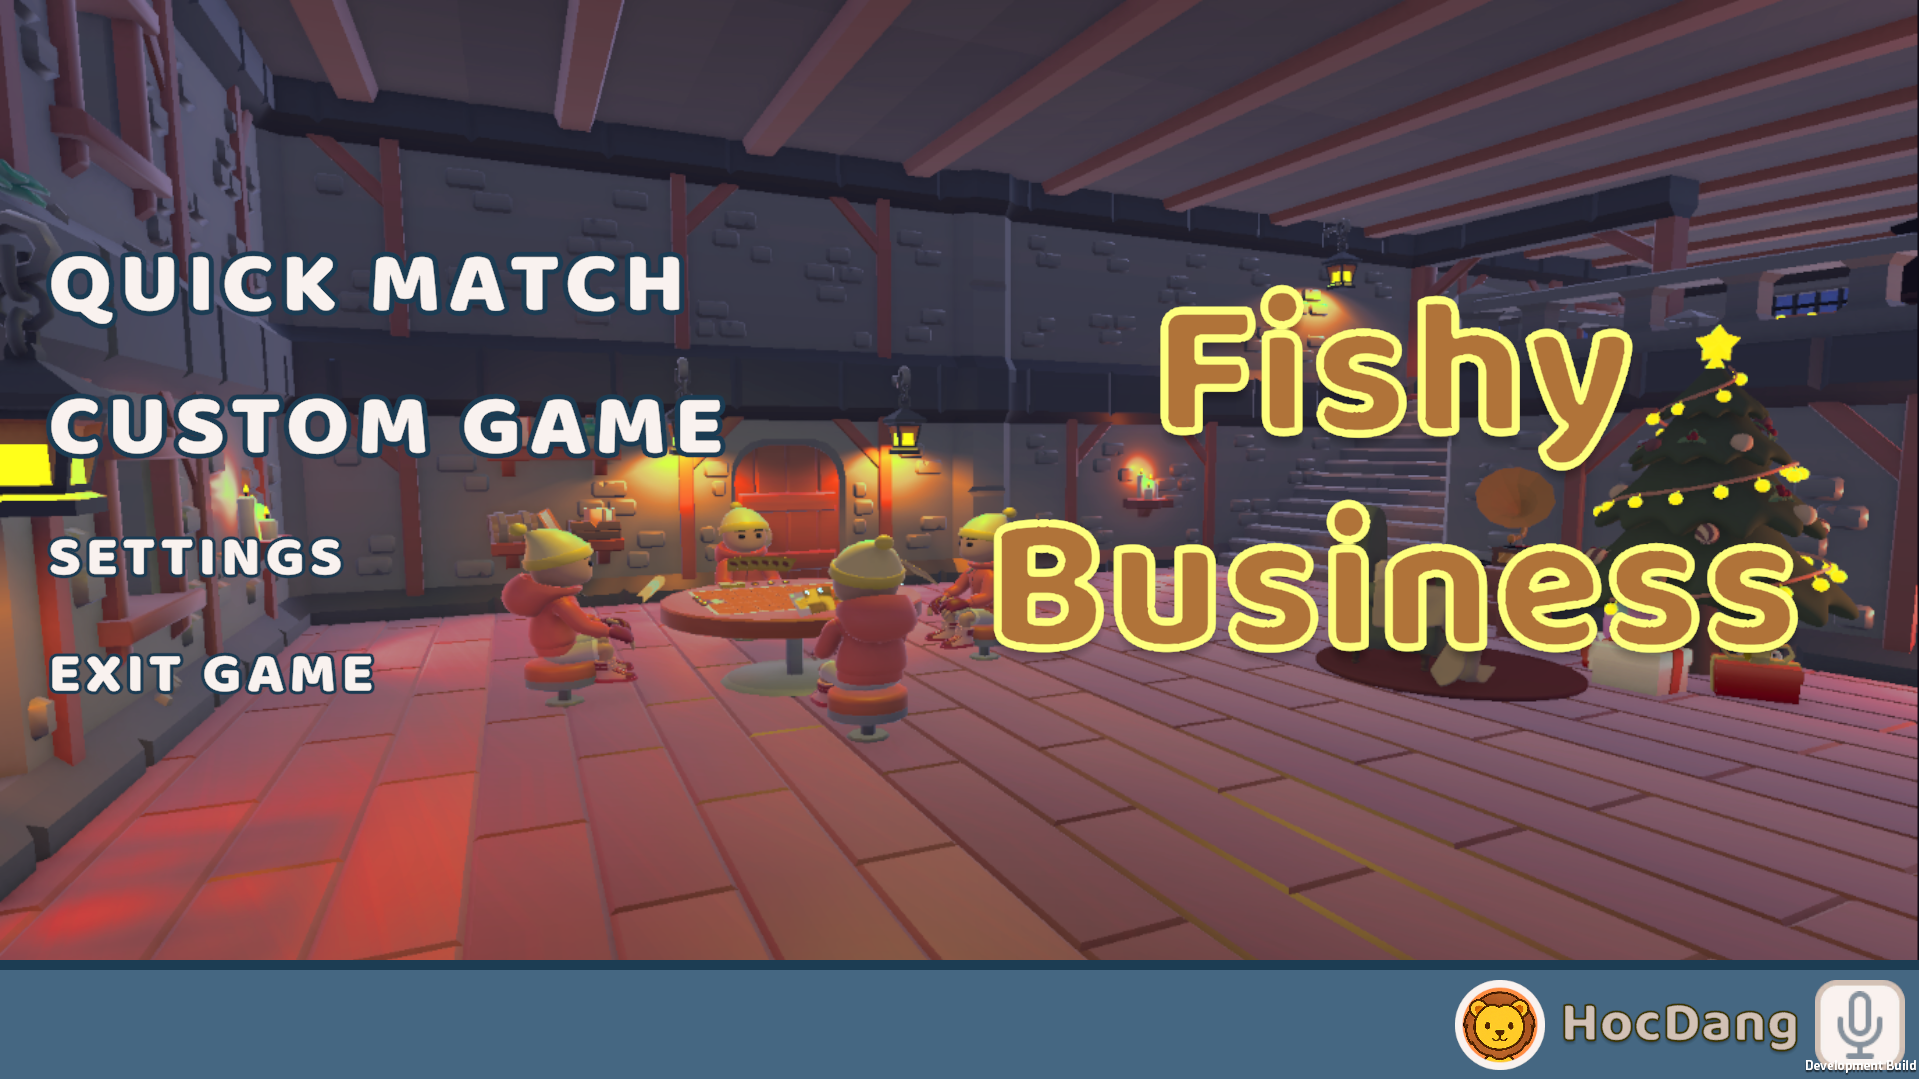
\includegraphics[width=0.75\linewidth]{10.Kết quả/images/MainMenu.png}
    \caption{Screenshot màn hình \textbf{Trang chủ} của trò chơi}
    \label{fig:game-object}
\end{figure}
Tại đây, người chơi có thể chọn:
\begin{itemize}
    \item \textbf{Quick Match} để tham gia vào 1 phòng chơi ngẫu nhiên (nếu có), 
    \item \textbf{Custom Game} để xem các phòng chơi hiện có và tham gia 1 phòng chơi trong số đó hoặc tạo 1 phòng chơi mới,
    \item  \textbf{Settings} để điều chỉnh các thống số hệ thống. 
    \item \textbf{Exit Game} để thoát trò chơi.
\end{itemize}

Ở góc dưới bên phải màn hình sẽ là thông tin của người chơi, người chơi có thể thay đổi thông tin bằng cách nhấn vào góc dưới đó.

\begin{figure} [H]
    \centering
    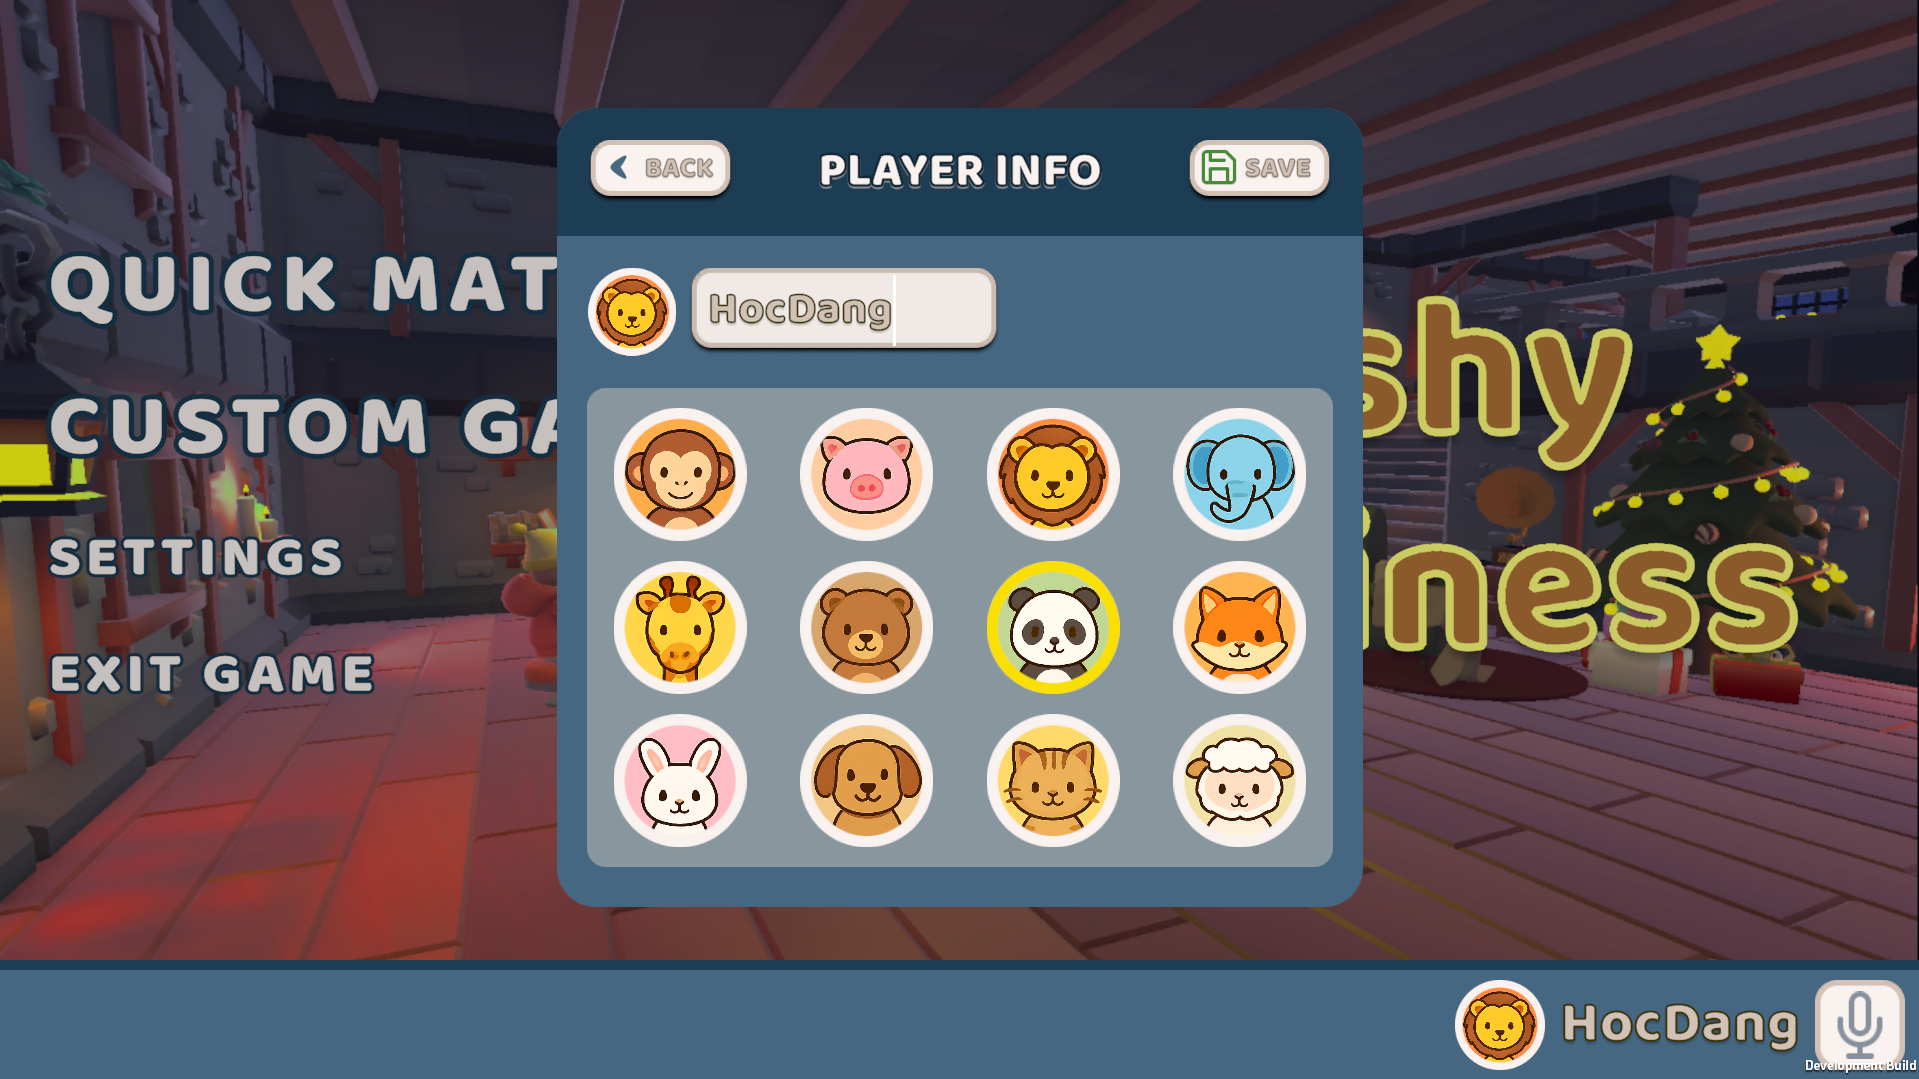
\includegraphics[width=0.75\linewidth]{10.Kết quả//images/ChangeName&Icon.png}
    \caption{Screenshot màn hình thay đổi tên và icon}
    \label{fig:placeholder}
\end{figure}

Sau khi nhấn nút \textbf{Custom Game} từ trang chủ, hệ thống hiển thị danh sách các phòng chơi hiện có như hình dưới đây:
\begin{figure}[H]
    \centering
    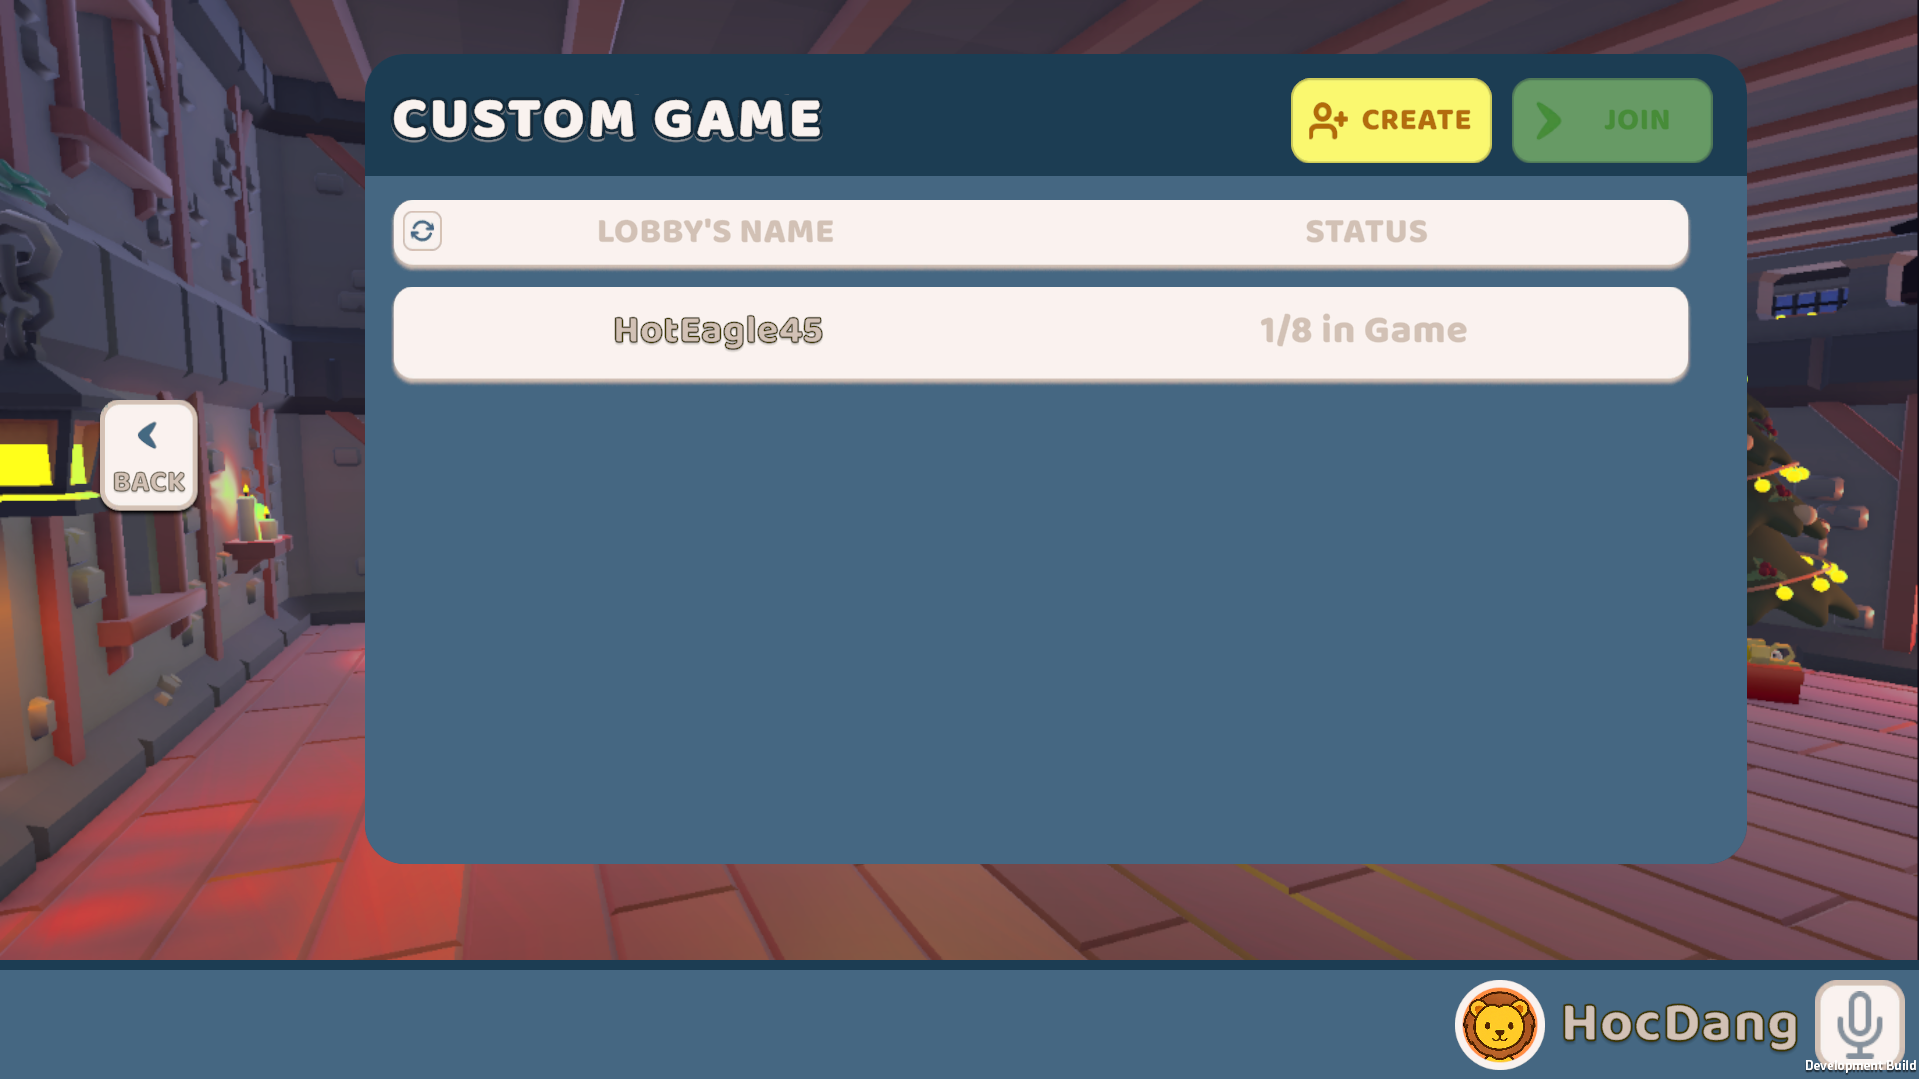
\includegraphics[width=0.75\linewidth]{10.Kết quả/images/CustomGame.png}
    \caption{Screenshot màn hình \textbf{Custom Game} của trò chơi}
    \label{fig:game-object}
\end{figure}
Ở giao diện này, người chơi có thể chọn 1 phòng chơi hiện có và chưa đầy người chơi (8 người) và nhấn nút \textbf{Join} để tham gia vào phòng chơi đó. Người chơi cũng có thể chọn \textbf{Create} để tạo phong chơi mới.
\begin{figure}[H]
    \centering
    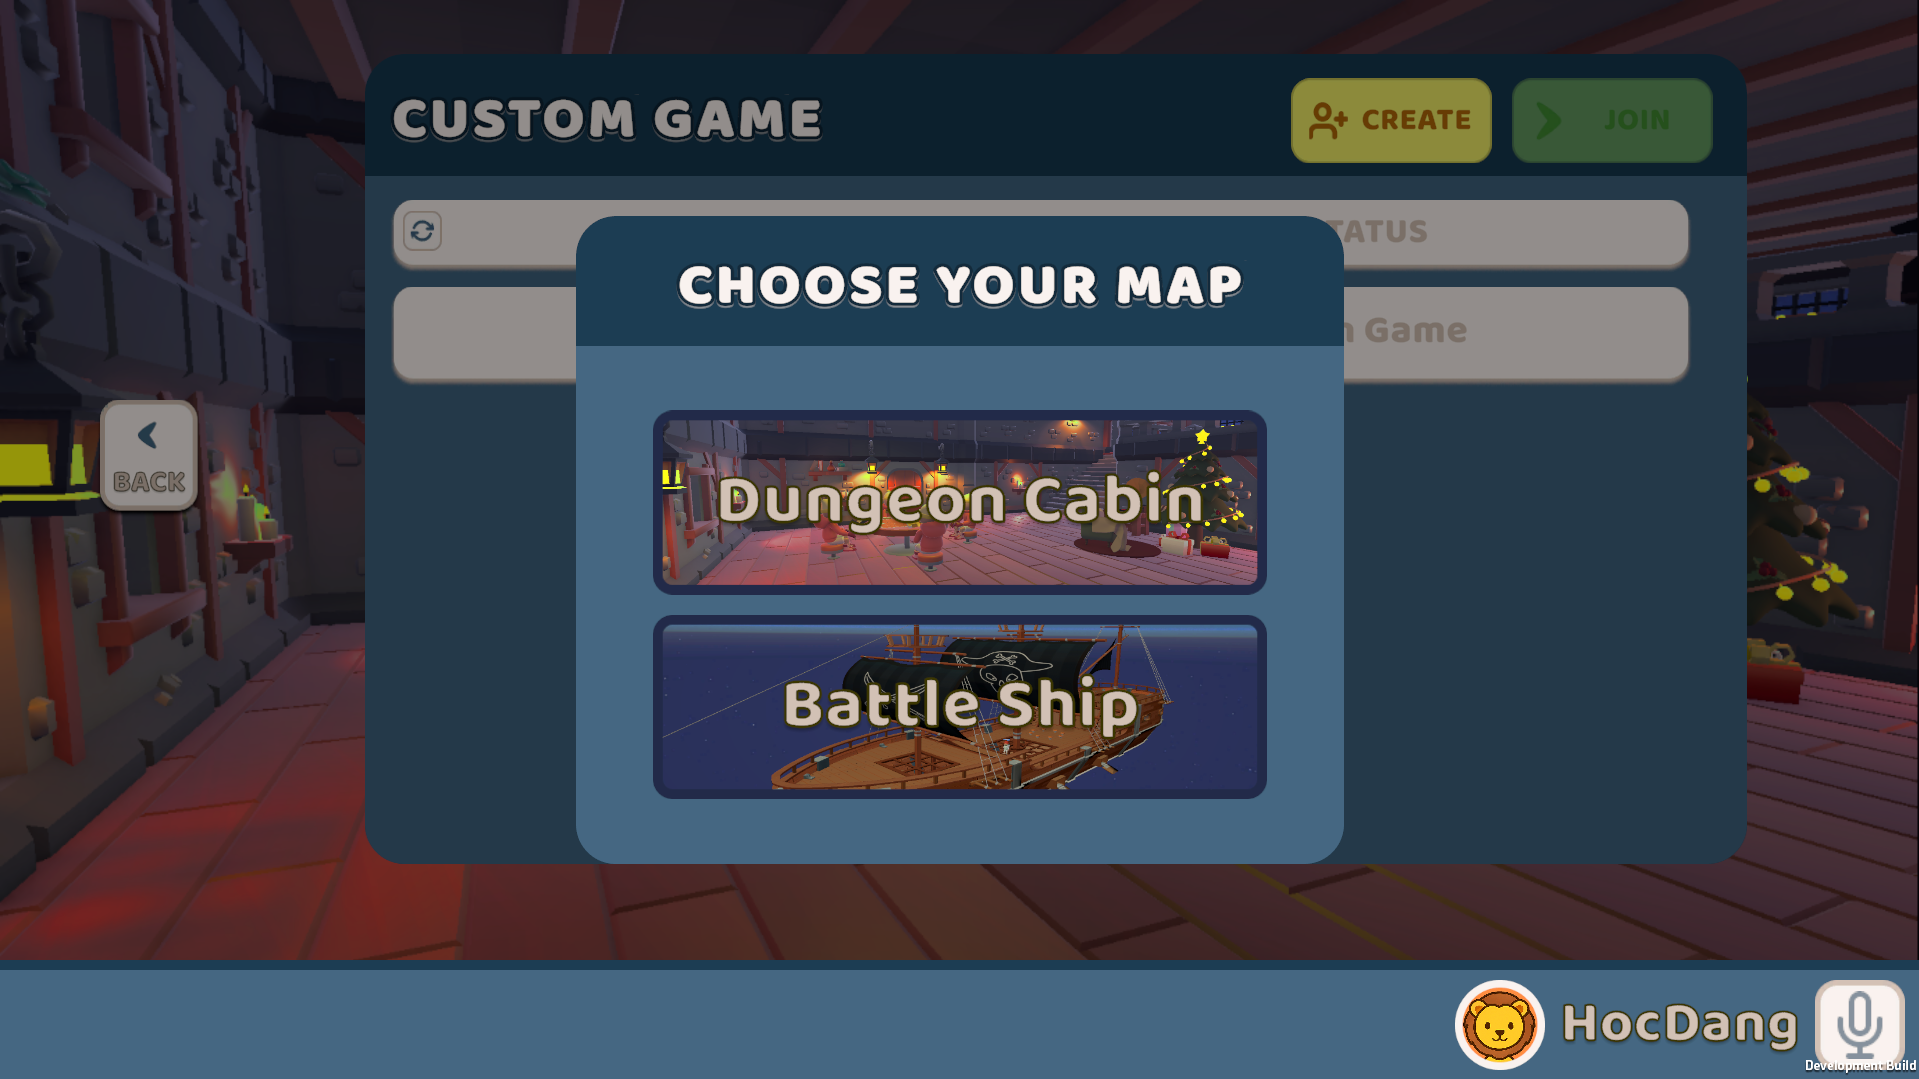
\includegraphics[width=0.75\linewidth]{10.Kết quả/images/ChooseMap.png}
    \caption{Screenshot màn hình chọn bản đồ của trò chơi}
    \label{fig:game-object}
\end{figure}
Tại đây, người chơi có thể chọn 1 trong 2 bản đồ để hoàn thành tạo 1 phòng chơi với bản đồ đó.
%\subsection{Phòng chơi}
Sau khi đã vào 1 phòng chơi bất kỳ, nhân vật của người chơi sẽ xuất hiện trong bản đồ.
\begin{figure}[H]
    \centering
    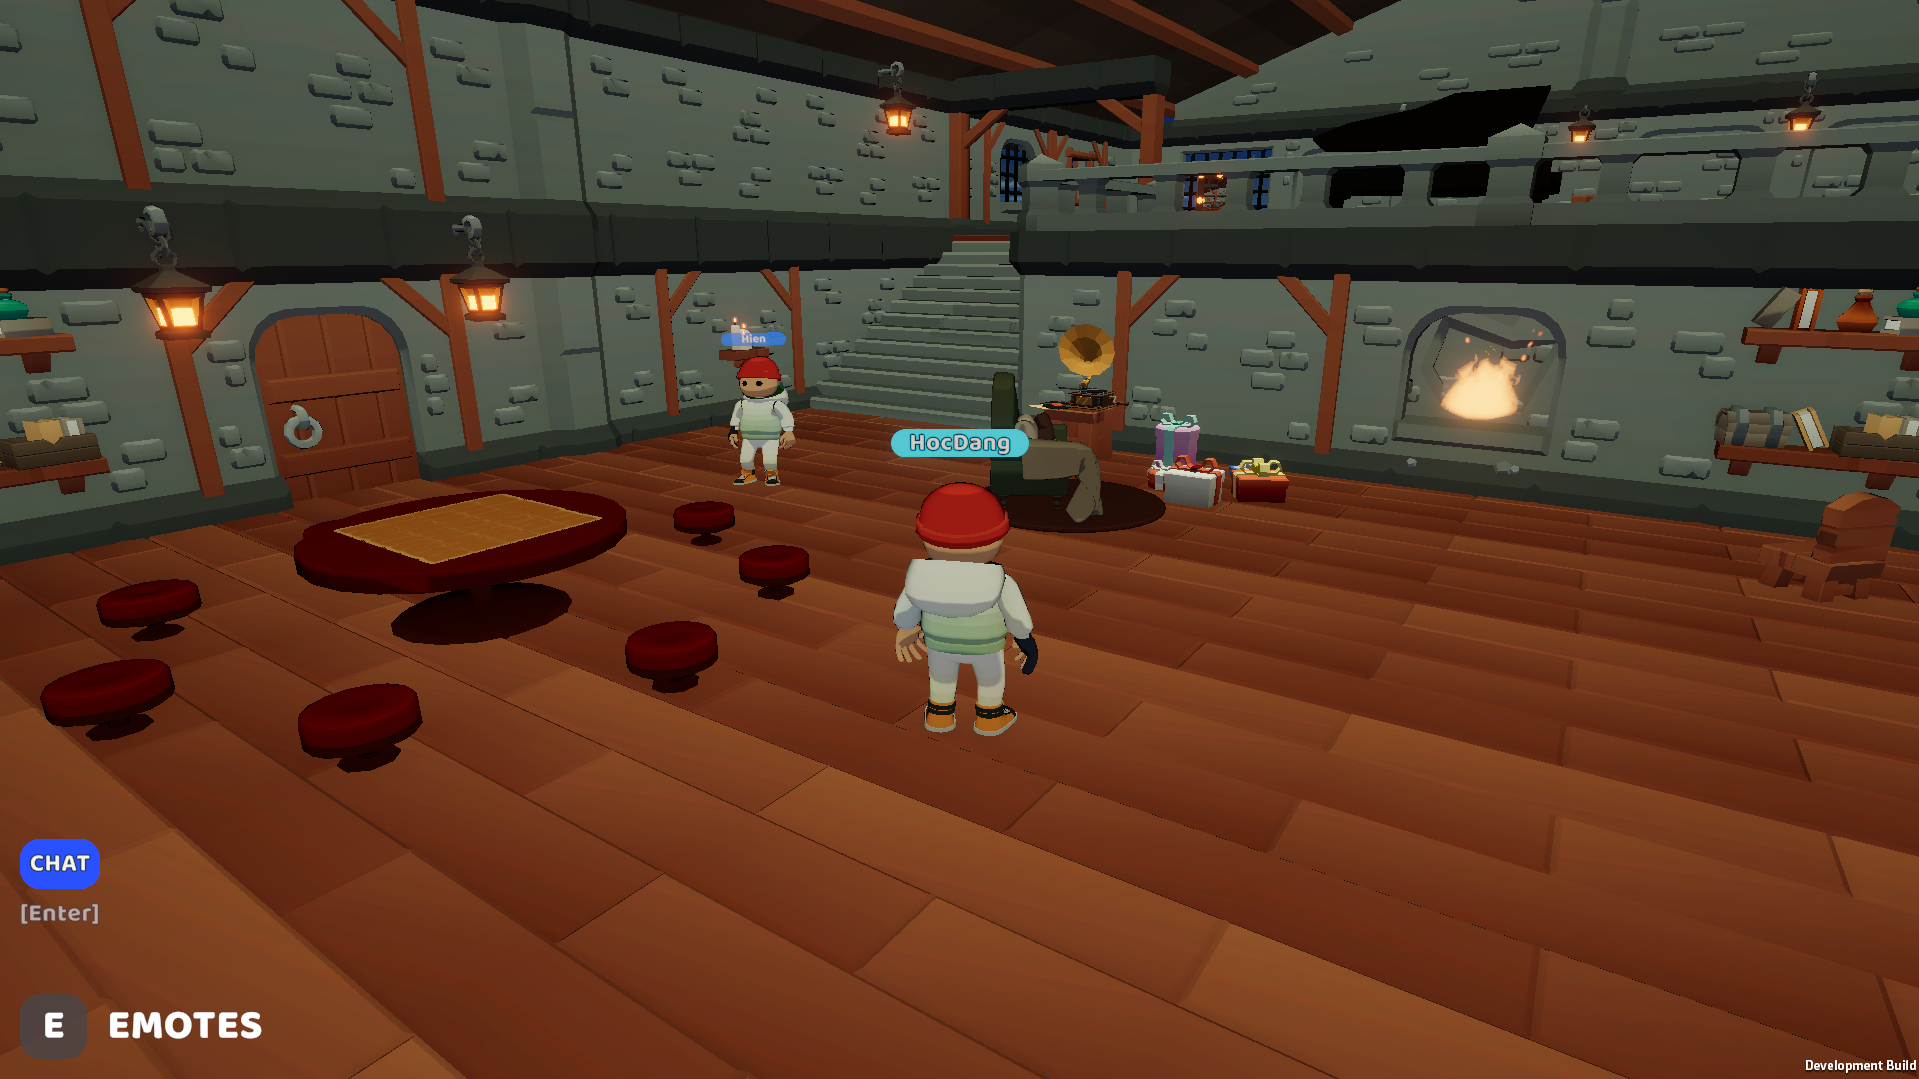
\includegraphics[width=0.75\linewidth]{10.Kết quả/images/DugeonMap.png}
    \caption{Screenshot màn hình bản đồ Dungeon Cabin của trò chơi}
    \label{fig:placeholder}
\end{figure}

\begin{figure}[H]
    \centering
    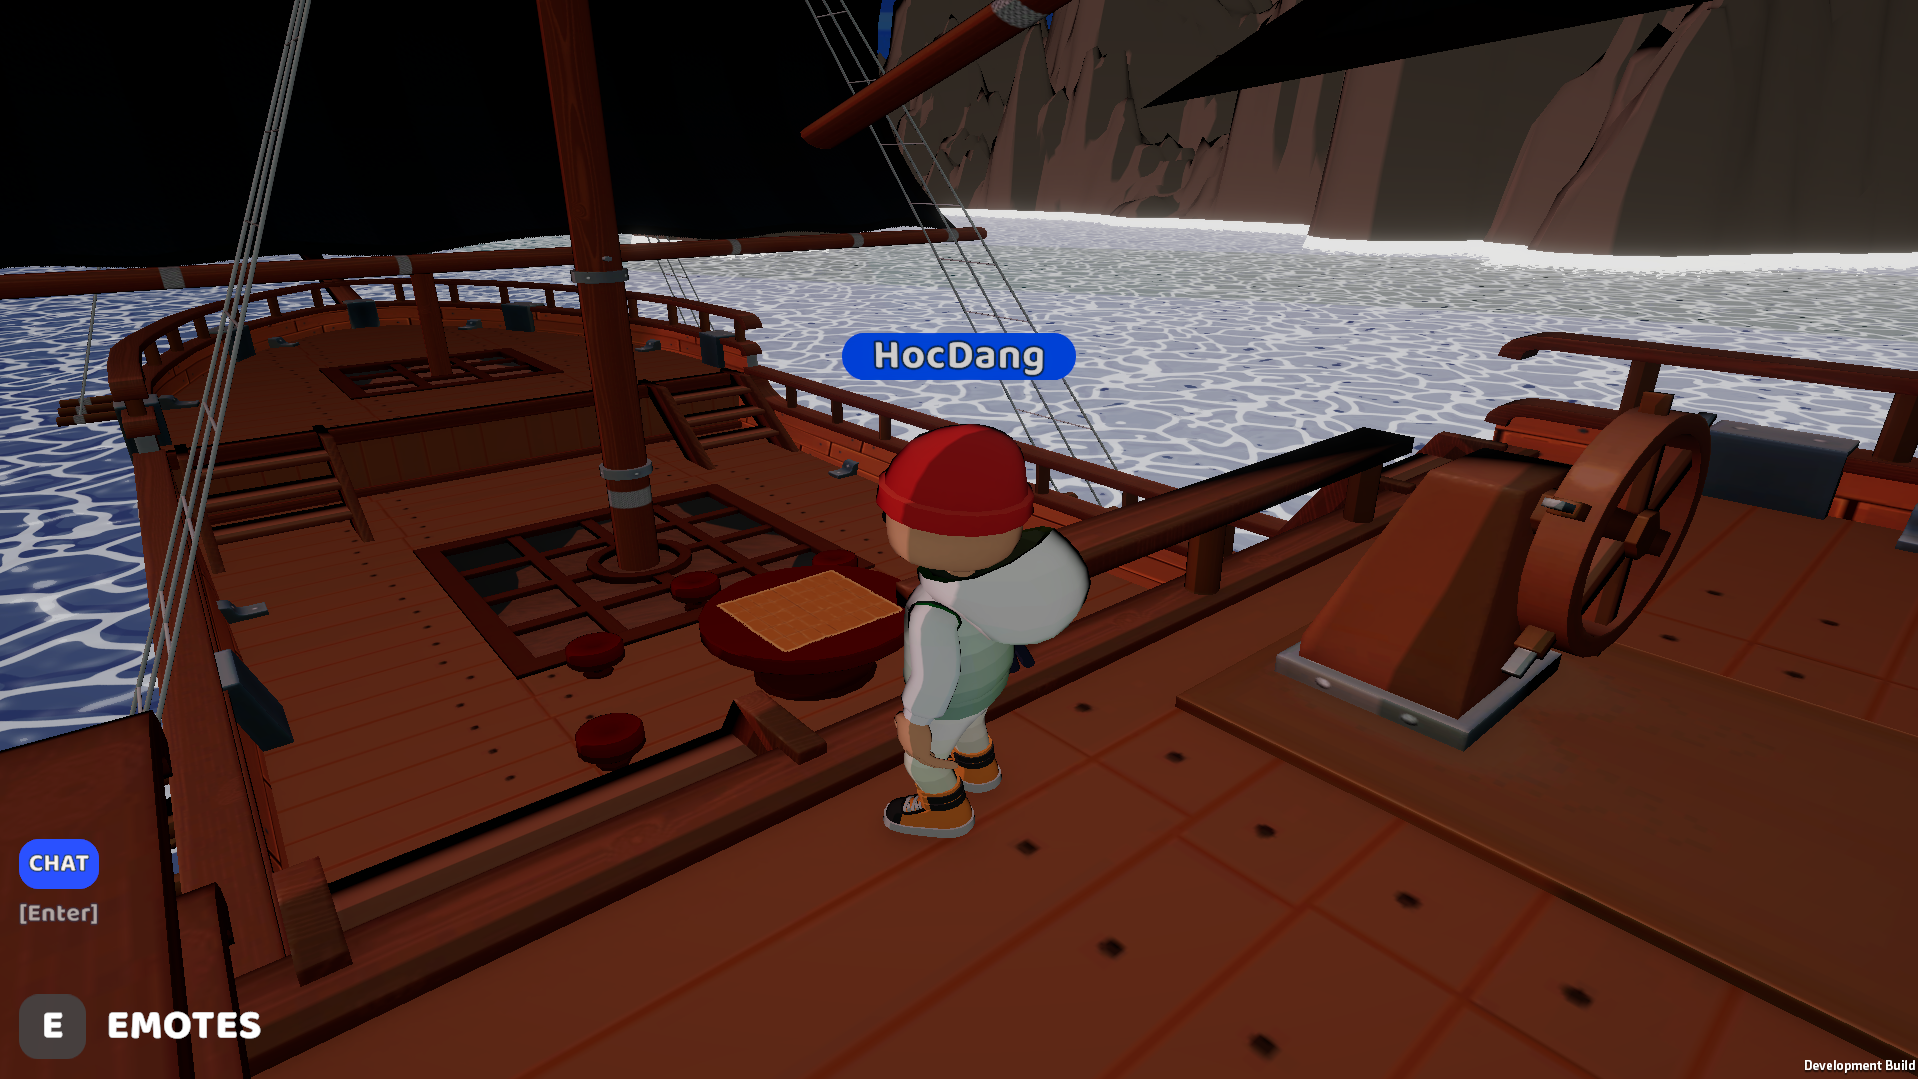
\includegraphics[width=0.75\linewidth]{10.Kết quả/images/BattleShipMap.png}
    \caption{Screenshot màn hình bản đồ Battle Ship của trò chơi}
    \label{fig:placeholder}
\end{figure}

Sau khi xuất hiện trong bản đồ, người chơi có thể đến gần các chiếc ghế xung quanh chiếc bàn và nhấn giữ nút "F" để ngồi vào bàn, khi đó sẽ hiện ra giao diện cấu hình cho game mode gồm 2 mdoe là classic (Saboteur gốc) và Day Night (Saboteur kết hợp với Ma sói).
\begin{figure}[H]
    \centering
    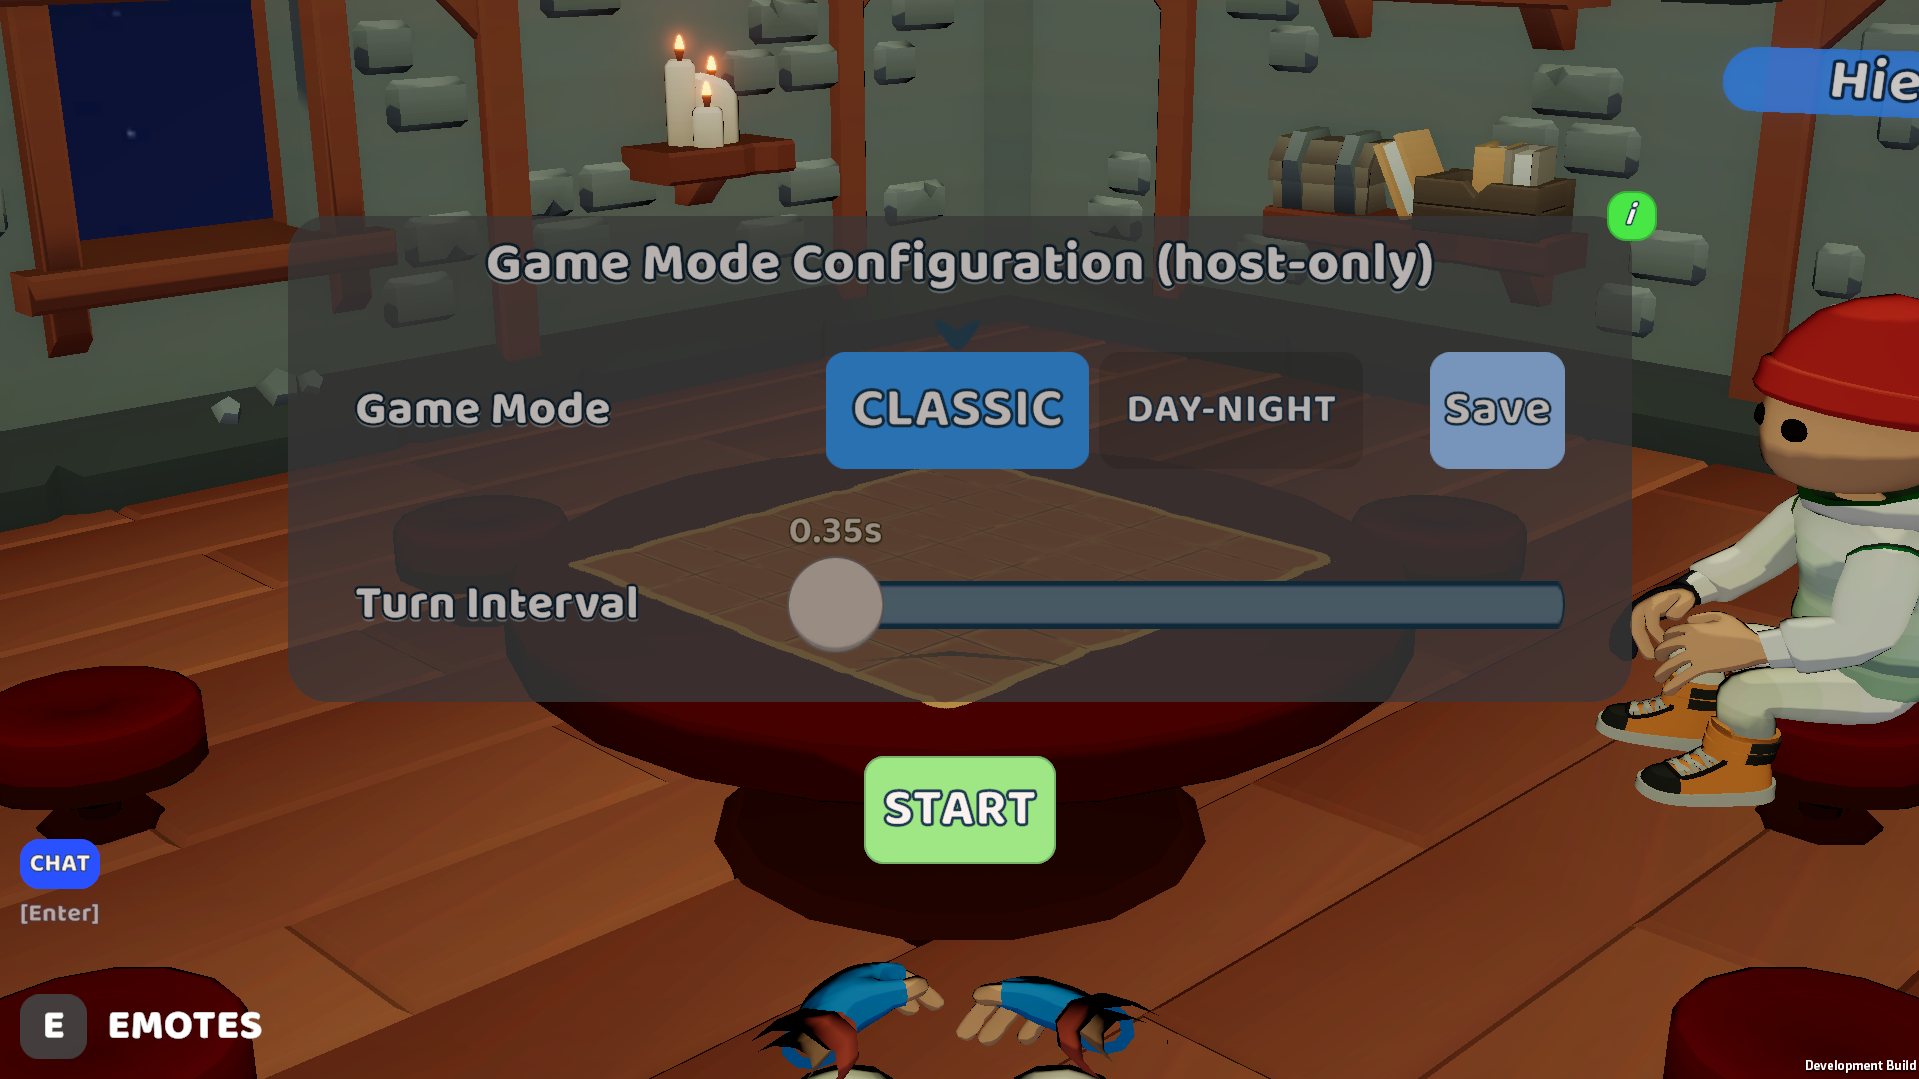
\includegraphics[width=0.75\linewidth]{10.Kết quả/images/ClassicConfig.png}
    \caption{Screenshot màn hình cấu hình Classic mode của trò chơi}
    \label{fig:placeholder}
\end{figure}

\begin{figure}[H]
    \centering
    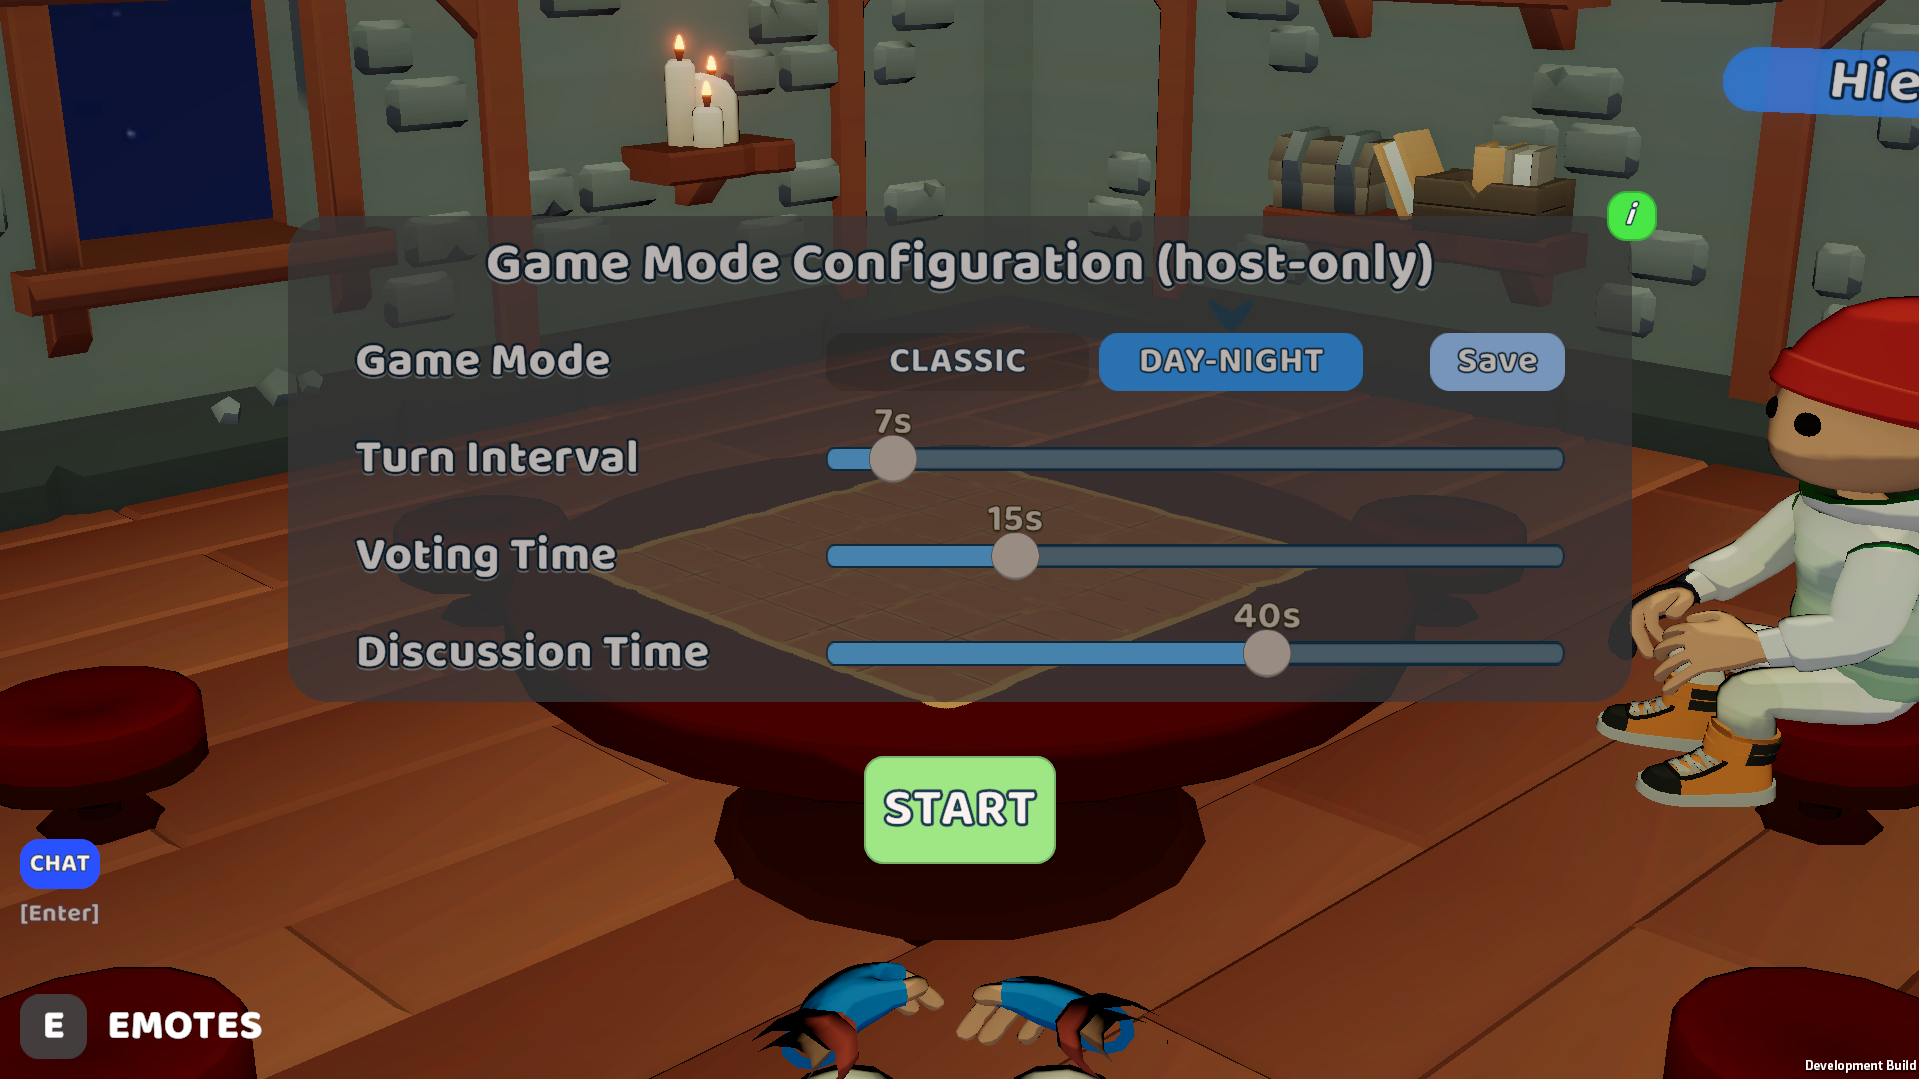
\includegraphics[width=0.75\linewidth]{10.Kết quả/images/DayNightConfig.png}
    \caption{Screenshot màn hình cấu hình Day Night mode của trò chơi}
    \label{fig:placeholder}
\end{figure}
Sau khi điều chỉnh thông số xong, người chơi chỉ cần nhấn nút "Save" và Start để bắt đầu vào trò chơi (chỉ chủ phòng mới có thể điều chỉnh thông số được).
\\
\begin{itemize}
    \item Classic Mode
        Tại đây, người chơi có thể chơi theo kim đồng hồ như Saboteur gốc.
        \begin{figure} [H]
            \centering
            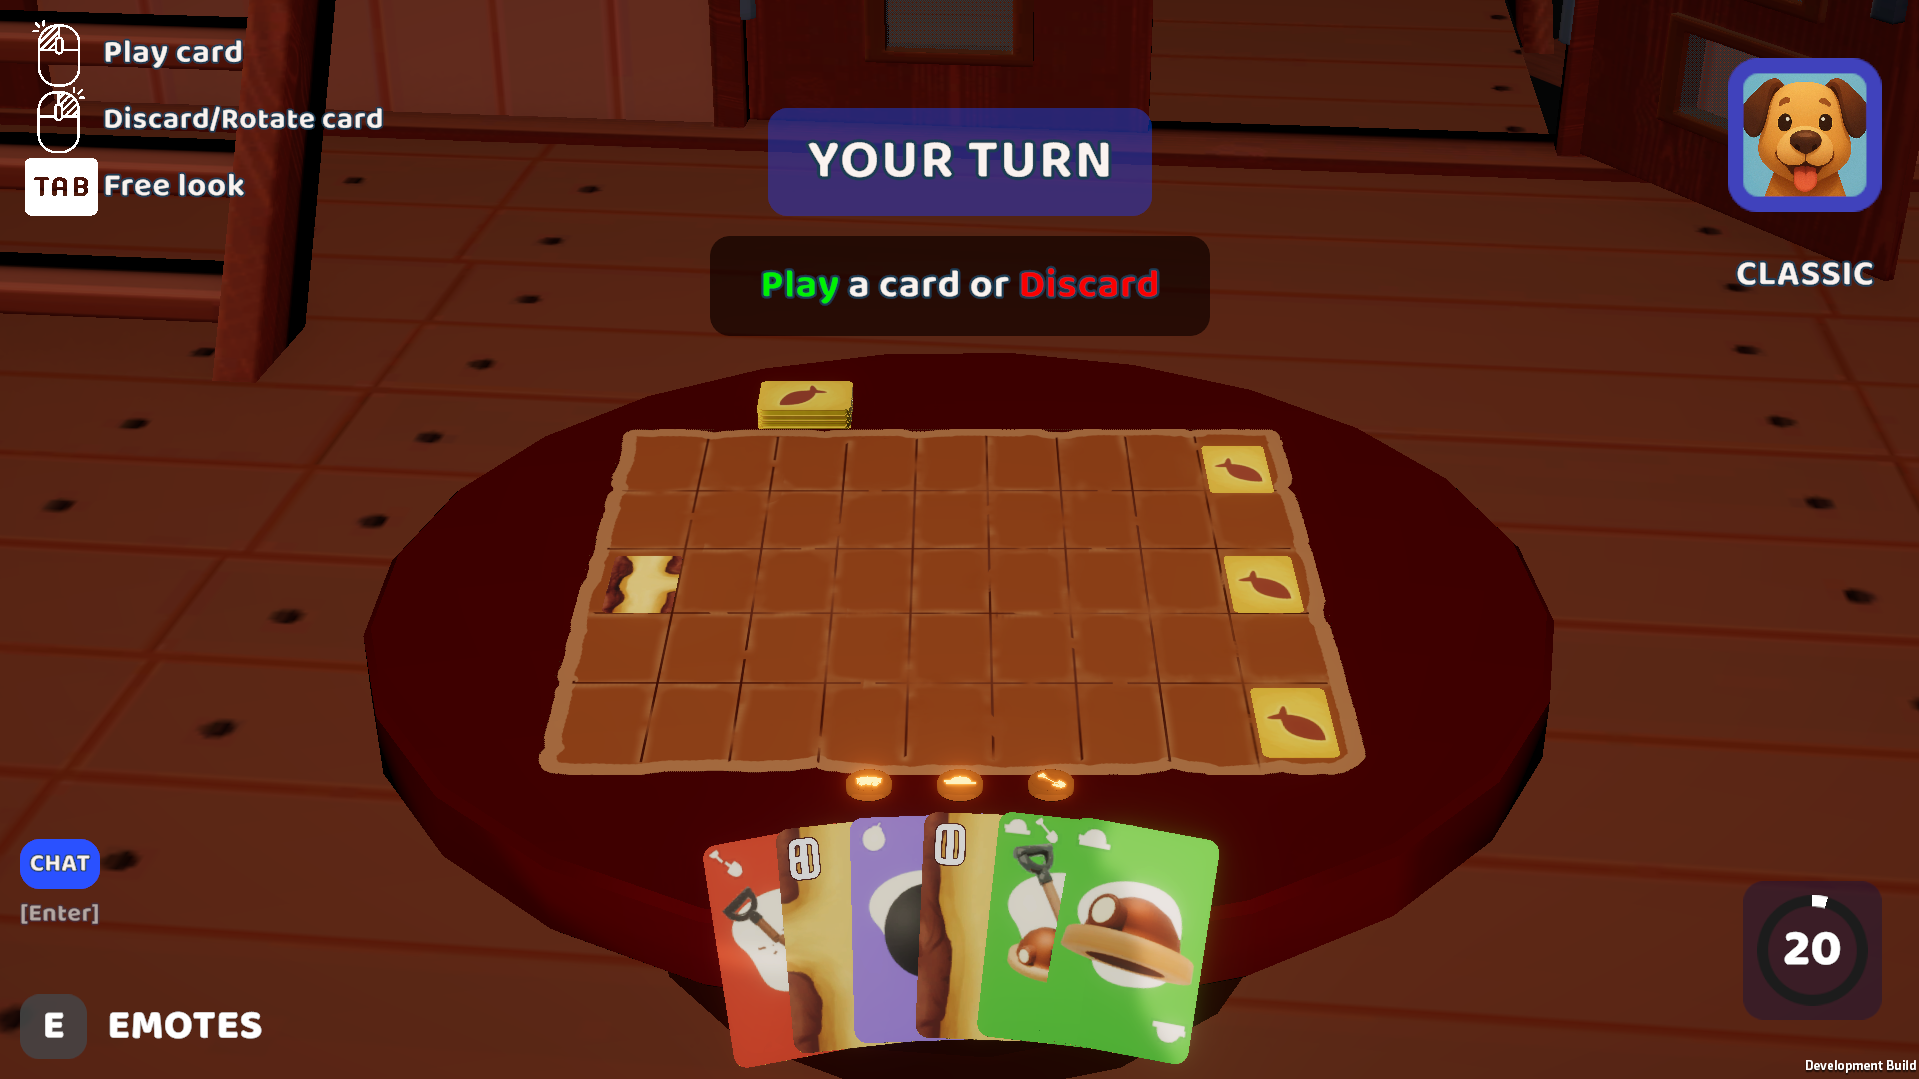
\includegraphics[width=0.75\linewidth]{10.Kết quả//images/ClassicMode.png}
            \caption{Screenshot màn hình bắt đầu Classic Mode của trò chơi}
            \label{fig:placeholder}
        \end{figure}
        Ở day phase, người chơi có thể thực hiện các hành động tự do như đặt đường, phá rối người khác, sử dụng các thẻ chức năng mà không sợ bị người khác thấy (trừ những người đã sử dụng thẻ nhìn xuyên đêm). Sau khi thực hiện 1 hành động xong thì sẽ kết thúc lượt.
    \item Day Night Mode
        \begin{figure} [H]
            \centering
            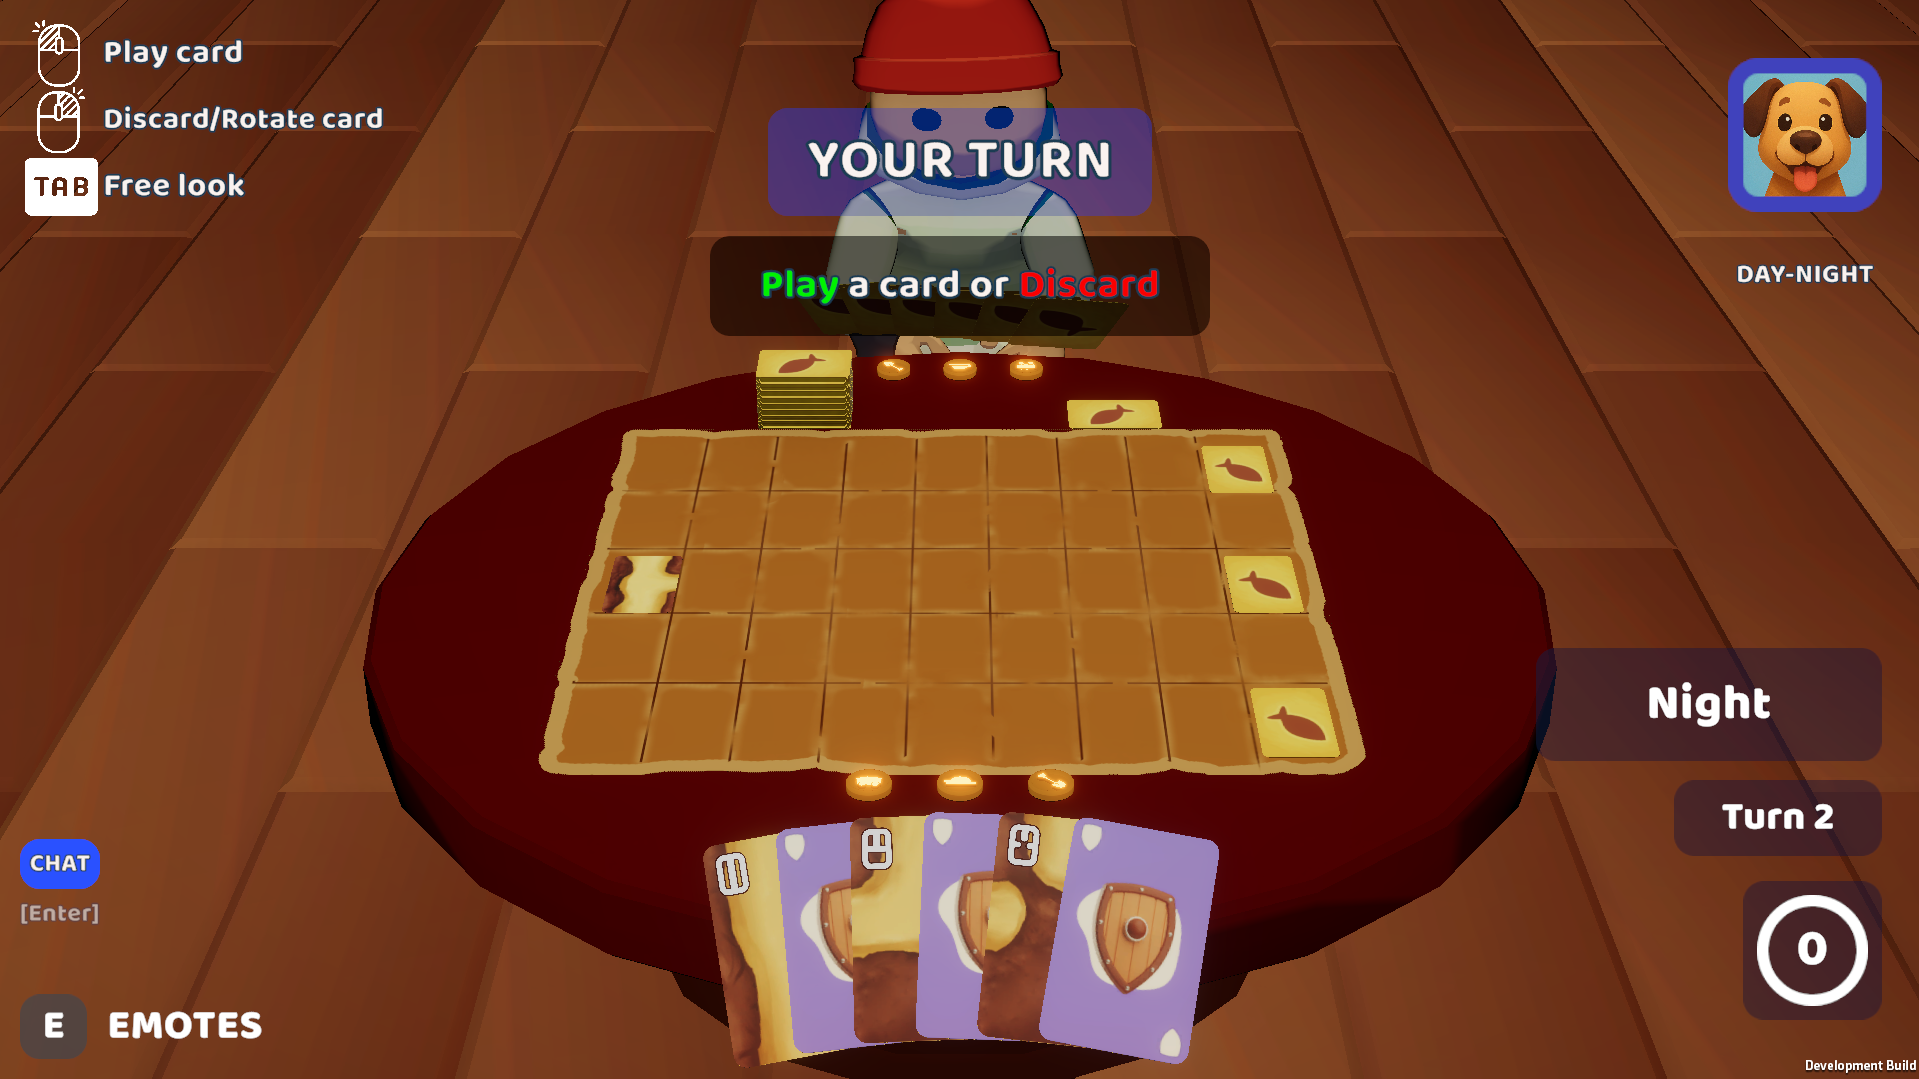
\includegraphics[width=0.75\linewidth]{10.Kết quả//images/DayPhase.png}
            \caption{Screenshot màn hình bắt đầu Day phase trong Day Night Mode của trò chơi}
            \label{fig:placeholder}
        \end{figure}
        Ở night phase, người chơi sẽ không thể nhìn được đang đến lượt ai hay ai đang làm gì, trừ khi đã sử dụng thẻ nhìn xuyên đêm. Chỉ khi sang phase mới như discussion hoặc đến lượt của bản thân gì mới có thể thấy được hiện trạng của board.
        \begin{figure} [H]
            \centering
            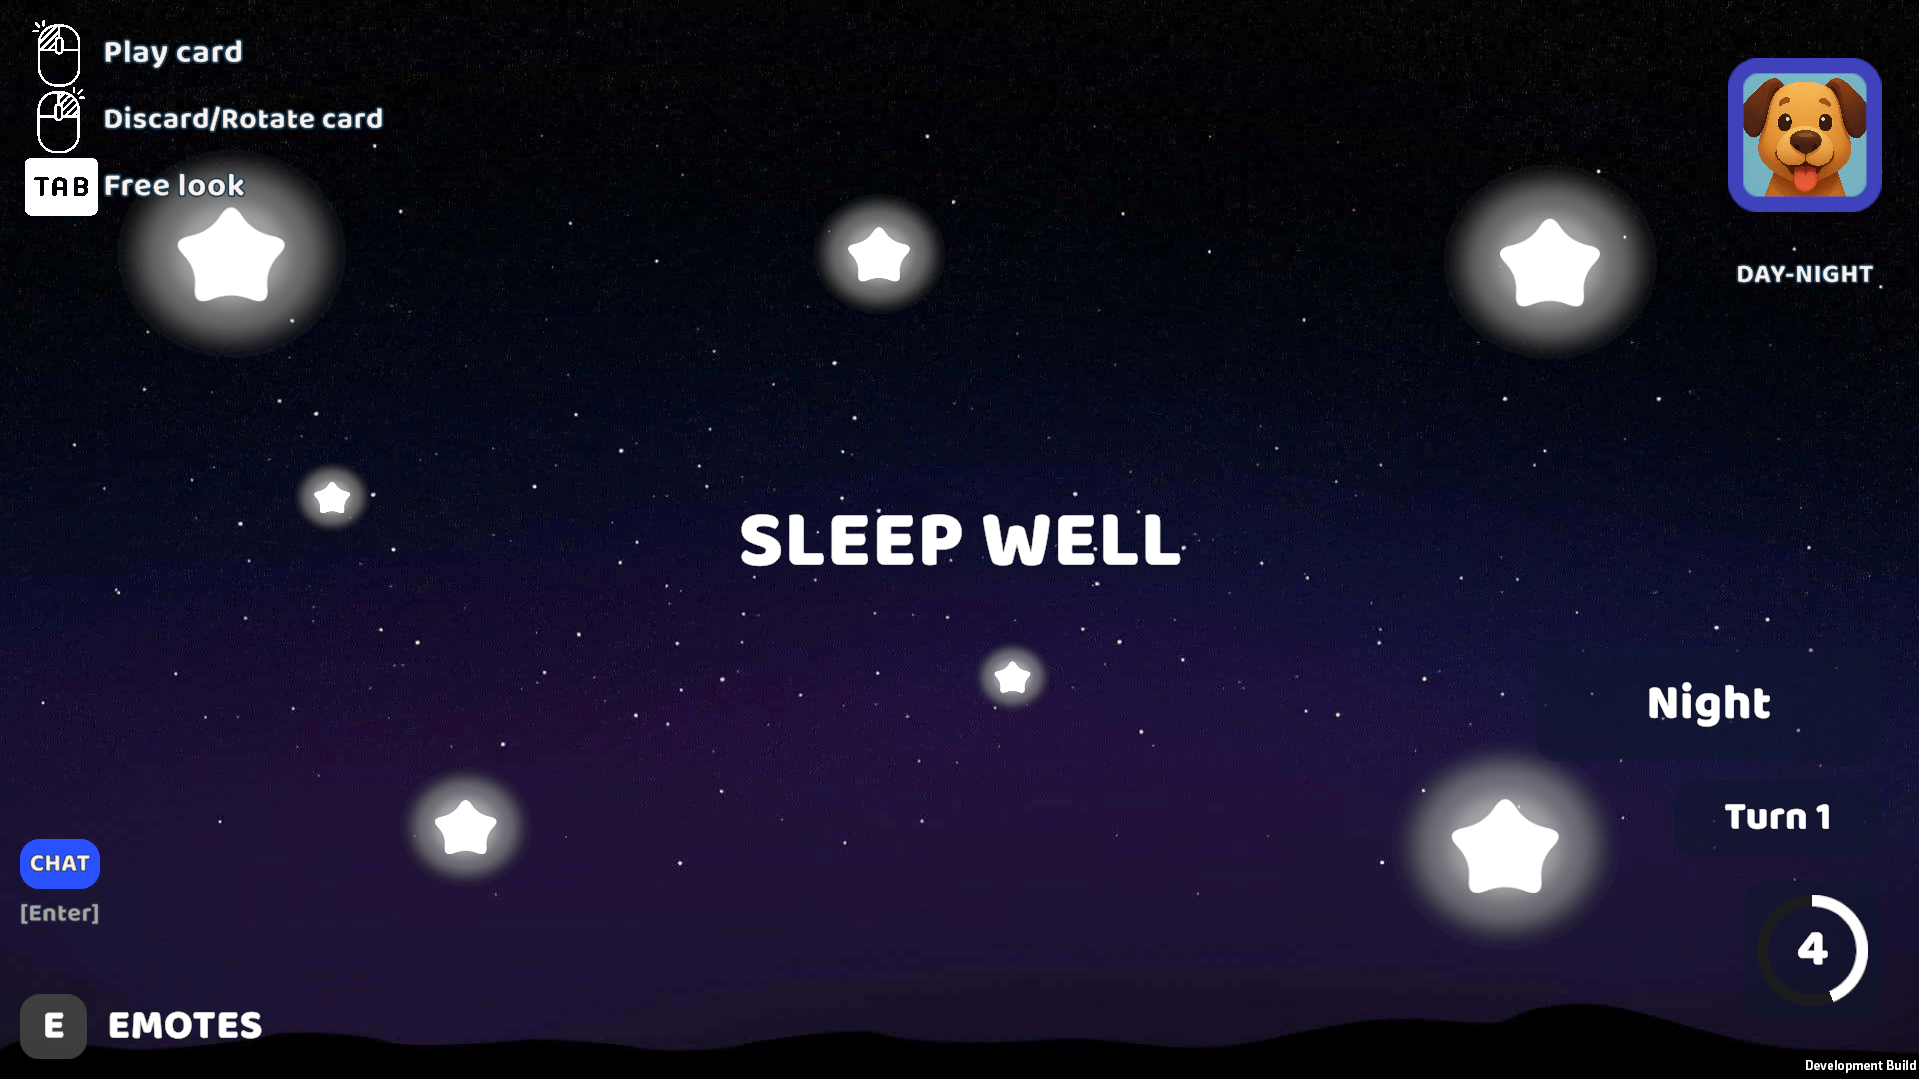
\includegraphics[width=0.75\linewidth]{10.Kết quả//images/NightPhase.png}
            \caption{Screenshot màn hình bắt đầu Night phase trong Day Night Mode của trò chơi}
            \label{fig:placeholder}
        \end{figure}
        Ở discussion phase, các người chơi có thể thấy được hiện trạng của board và thảo luận xem ai đã phá rối hay có vấn đề gì để có thể tiếp tục voting phase.
        
        \begin{figure} [H]
            \centering
            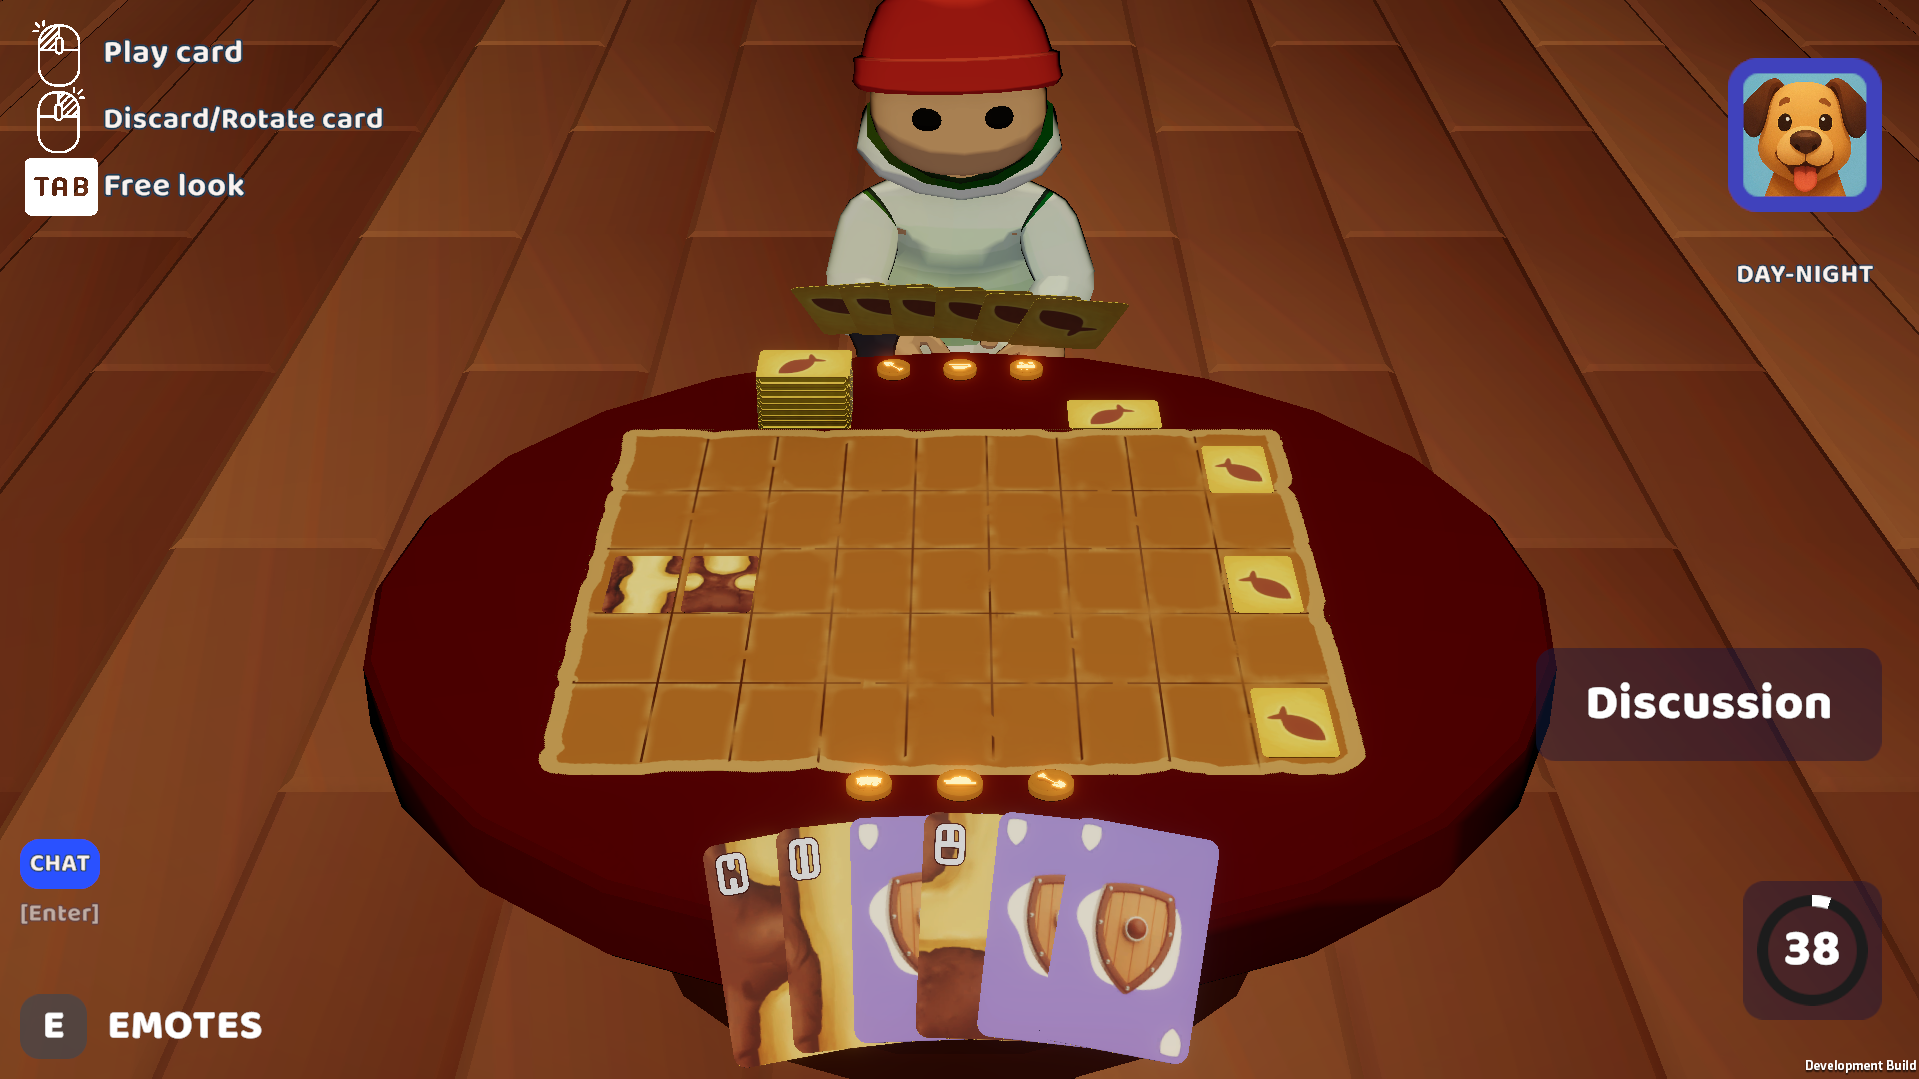
\includegraphics[width=0.75\linewidth]{10.Kết quả//images/DiscussionPhase.png}
            \caption{Screenshot màn hình bắt đầu Discussion phase trong Day Night Mode của trò chơi}
            \label{fig:placeholder}
        \end{figure}
        Ở voting phase, các người chơi có thể bầu chọn những ai mà mình nghi ngờ nhằm mục đích cấm 1 lượt chơi của người đó ở đêm kế tiếp.
        \begin{figure} [H]
            \centering
            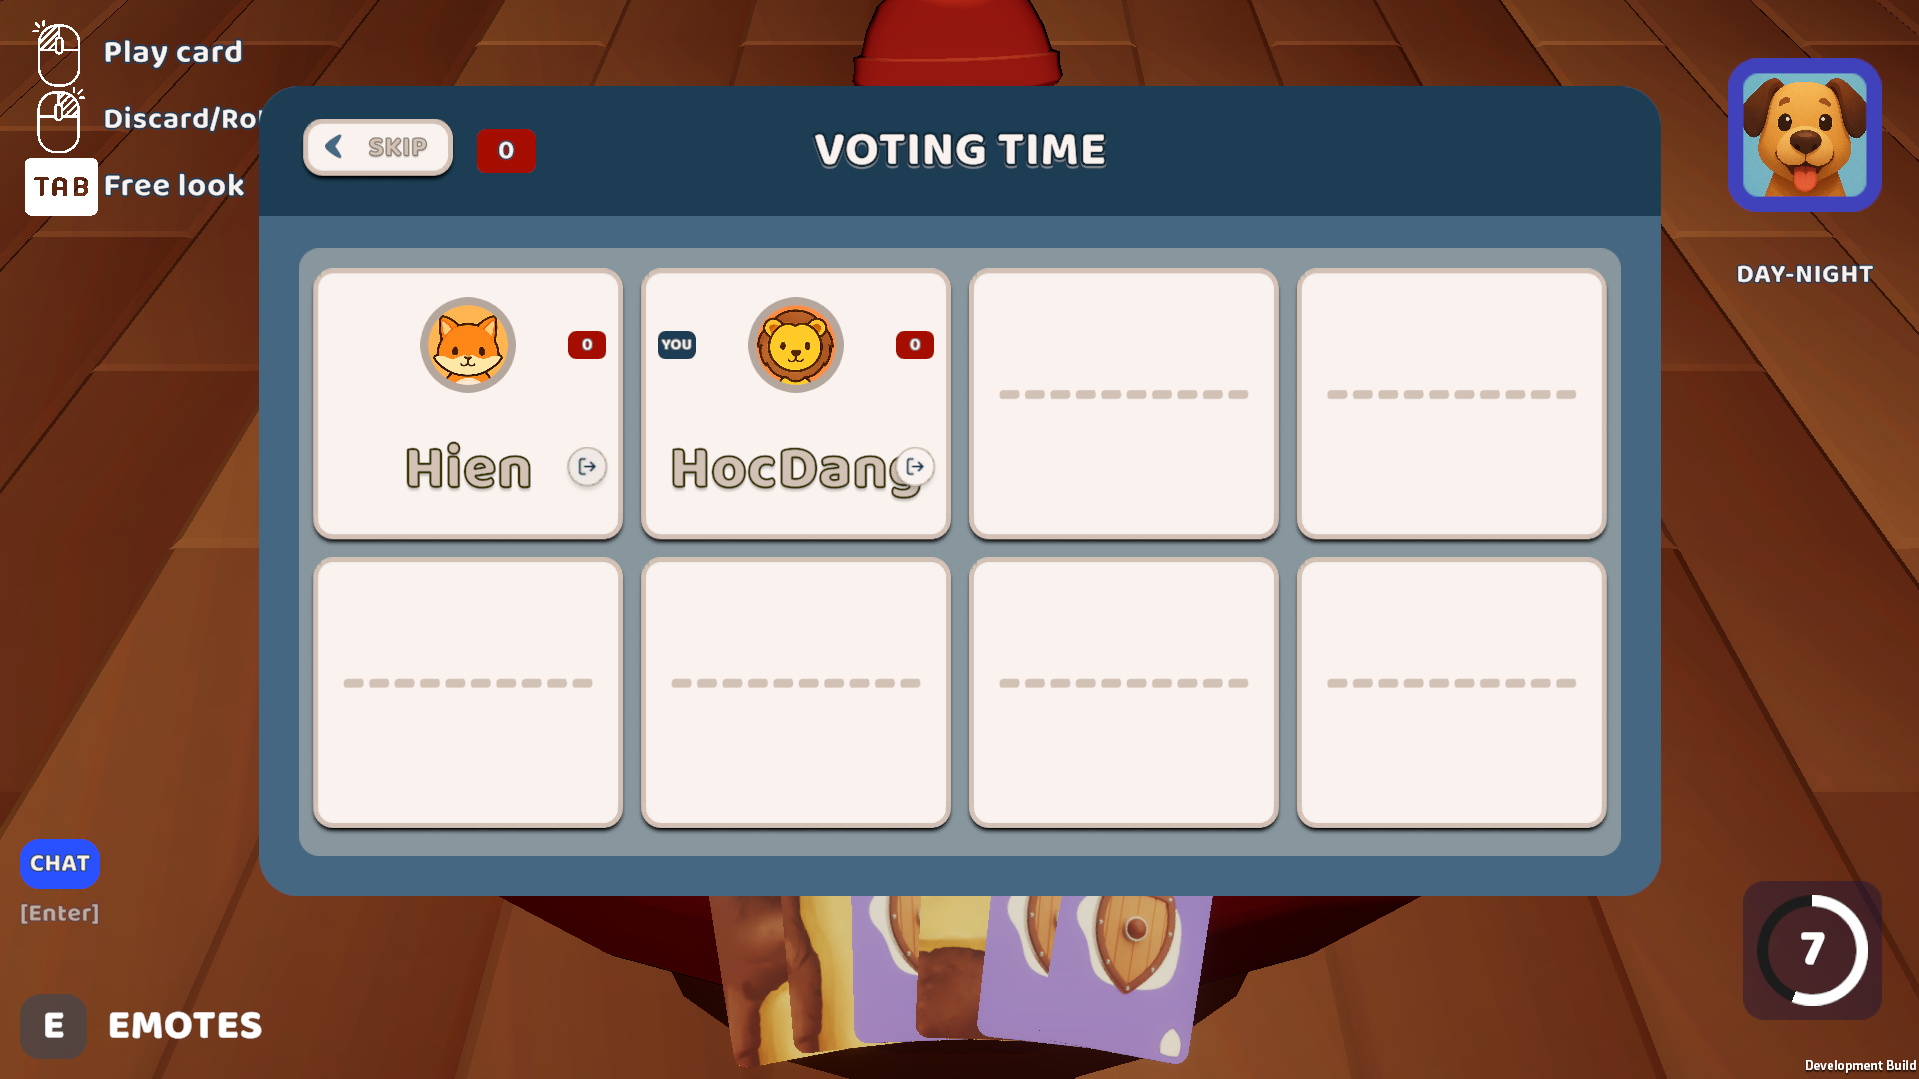
\includegraphics[width=0.75\linewidth]{10.Kết quả//images/VotingPhase.png}
            \caption{Screenshot màn hình bắt đầu Voting phase trong Day Night Mode của trò chơi}
            \label{fig:placeholder}
        \end{figure}
\end{itemize}

\subsubsection{Menu}
Người chơi có thể mở giao diện Menu bằng cách nhấn nút "Esc" để có thể xem thông tin phòng chơi, thông tin trò chơi, ...
\begin{figure}[H]
    \centering
    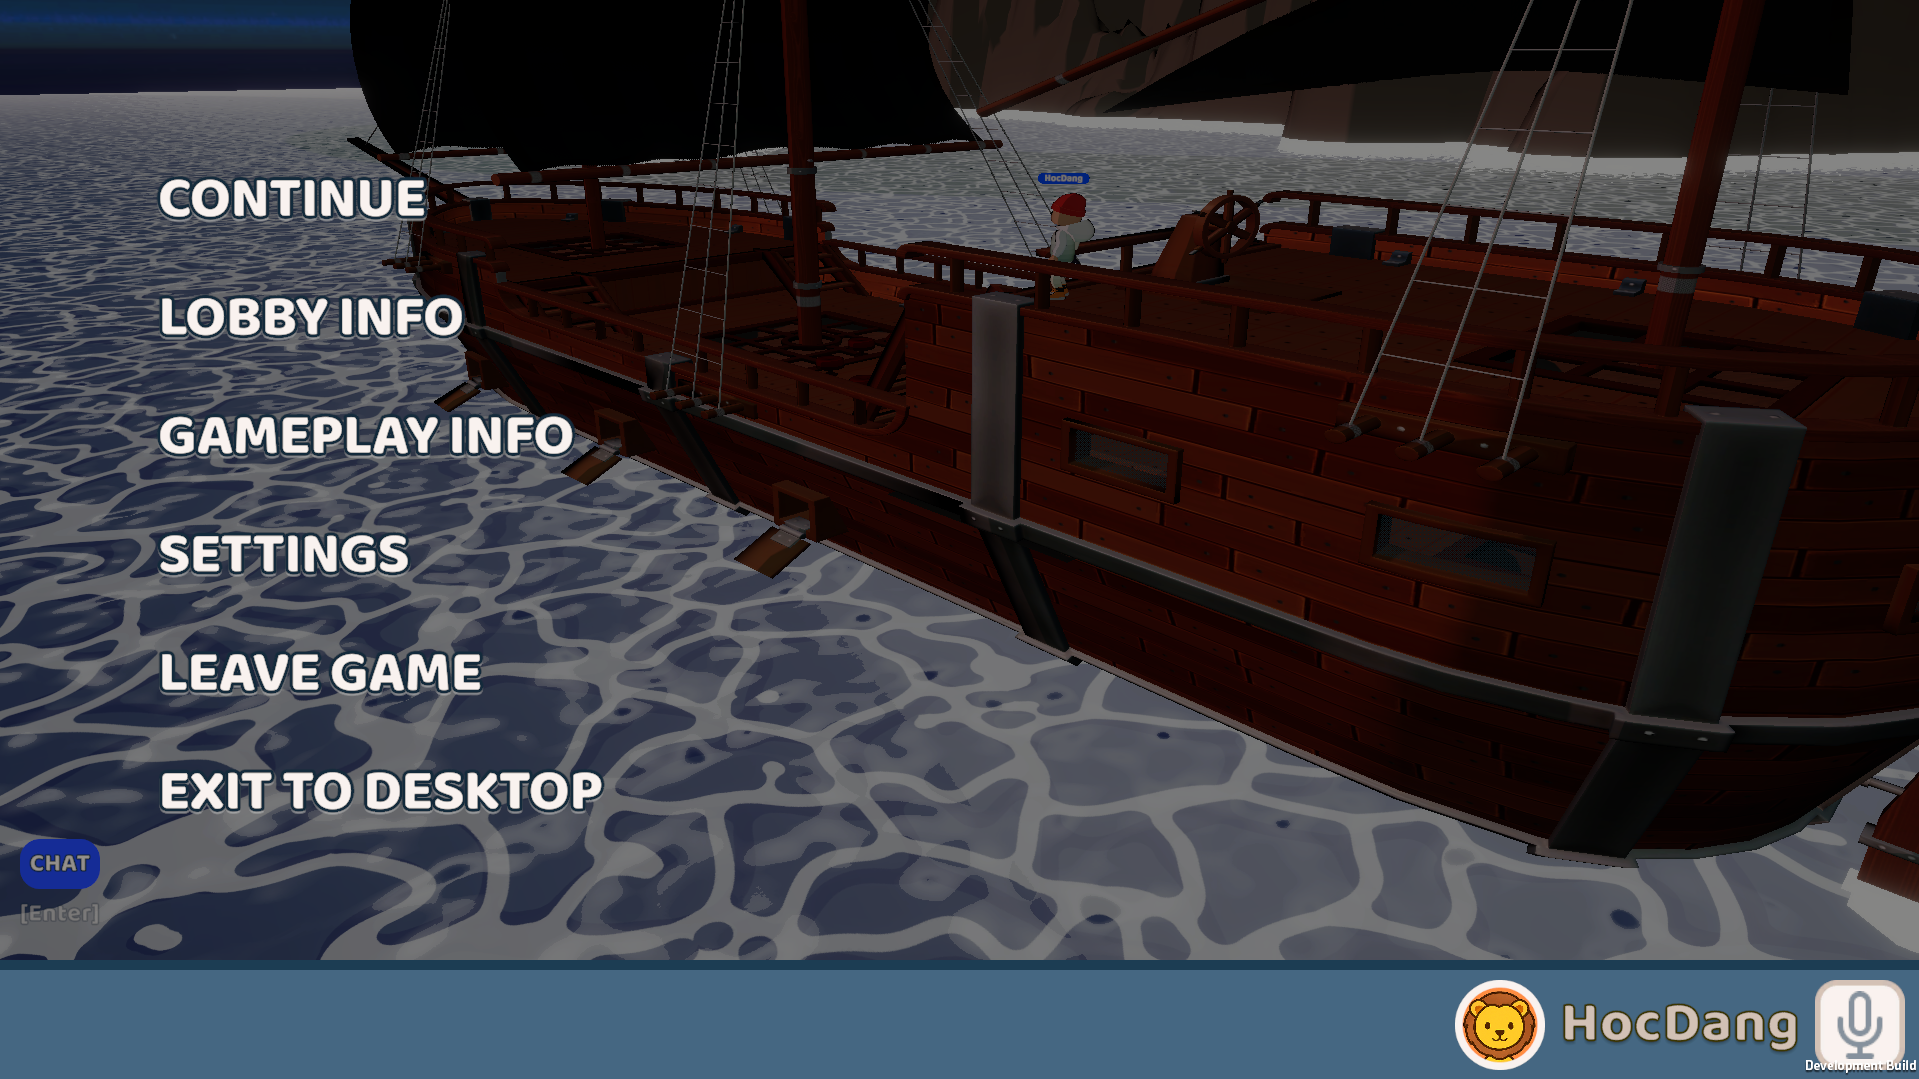
\includegraphics[width=0.75\linewidth]{10.Kết quả/images/MenuLobby.png}
    \caption{Screenshot màn hình Menu Lobby của trò chơi}
    \label{fig:placeholder}
\end{figure}
Người chơi có thể nhấn vào Lobby Info để xem thông tin phòng chơi như: có những ai, kết thúc game (nếu đang chơi board game), ... hoặc cũng có thể kick một người chơi ra khỏi phòng (chỉ chủ phòng mới làm được).
\begin{figure}[H]
    \centering
    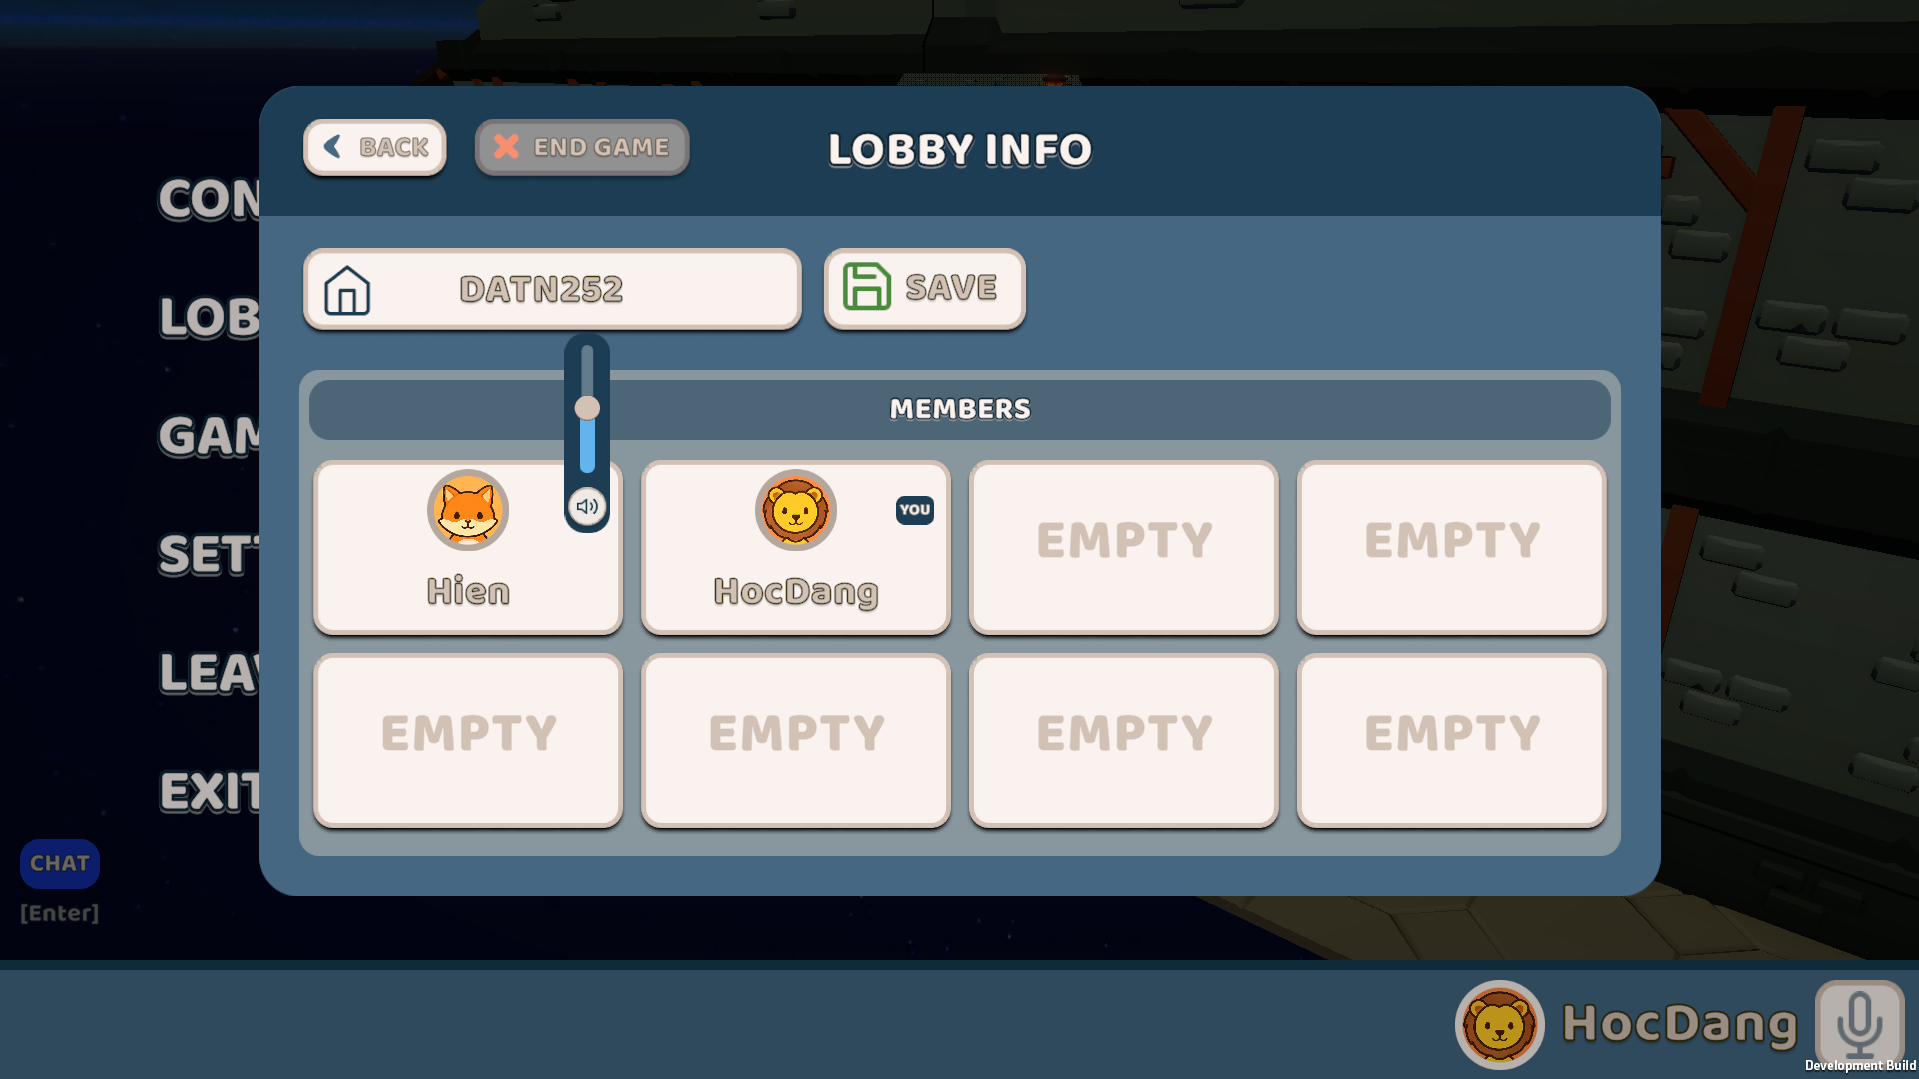
\includegraphics[width=0.75\linewidth]{10.Kết quả/images/LobbyInfo.png}
    \caption{Screenshot màn hình Lobby Info của trò chơi}
    \label{fig:placeholder}
\end{figure}
Người chơi cũng có thể nhấn vào Gameplay Info để xem luật chơi, các chức năng của các lá bài, ...
\begin{figure}[H]
    \centering
    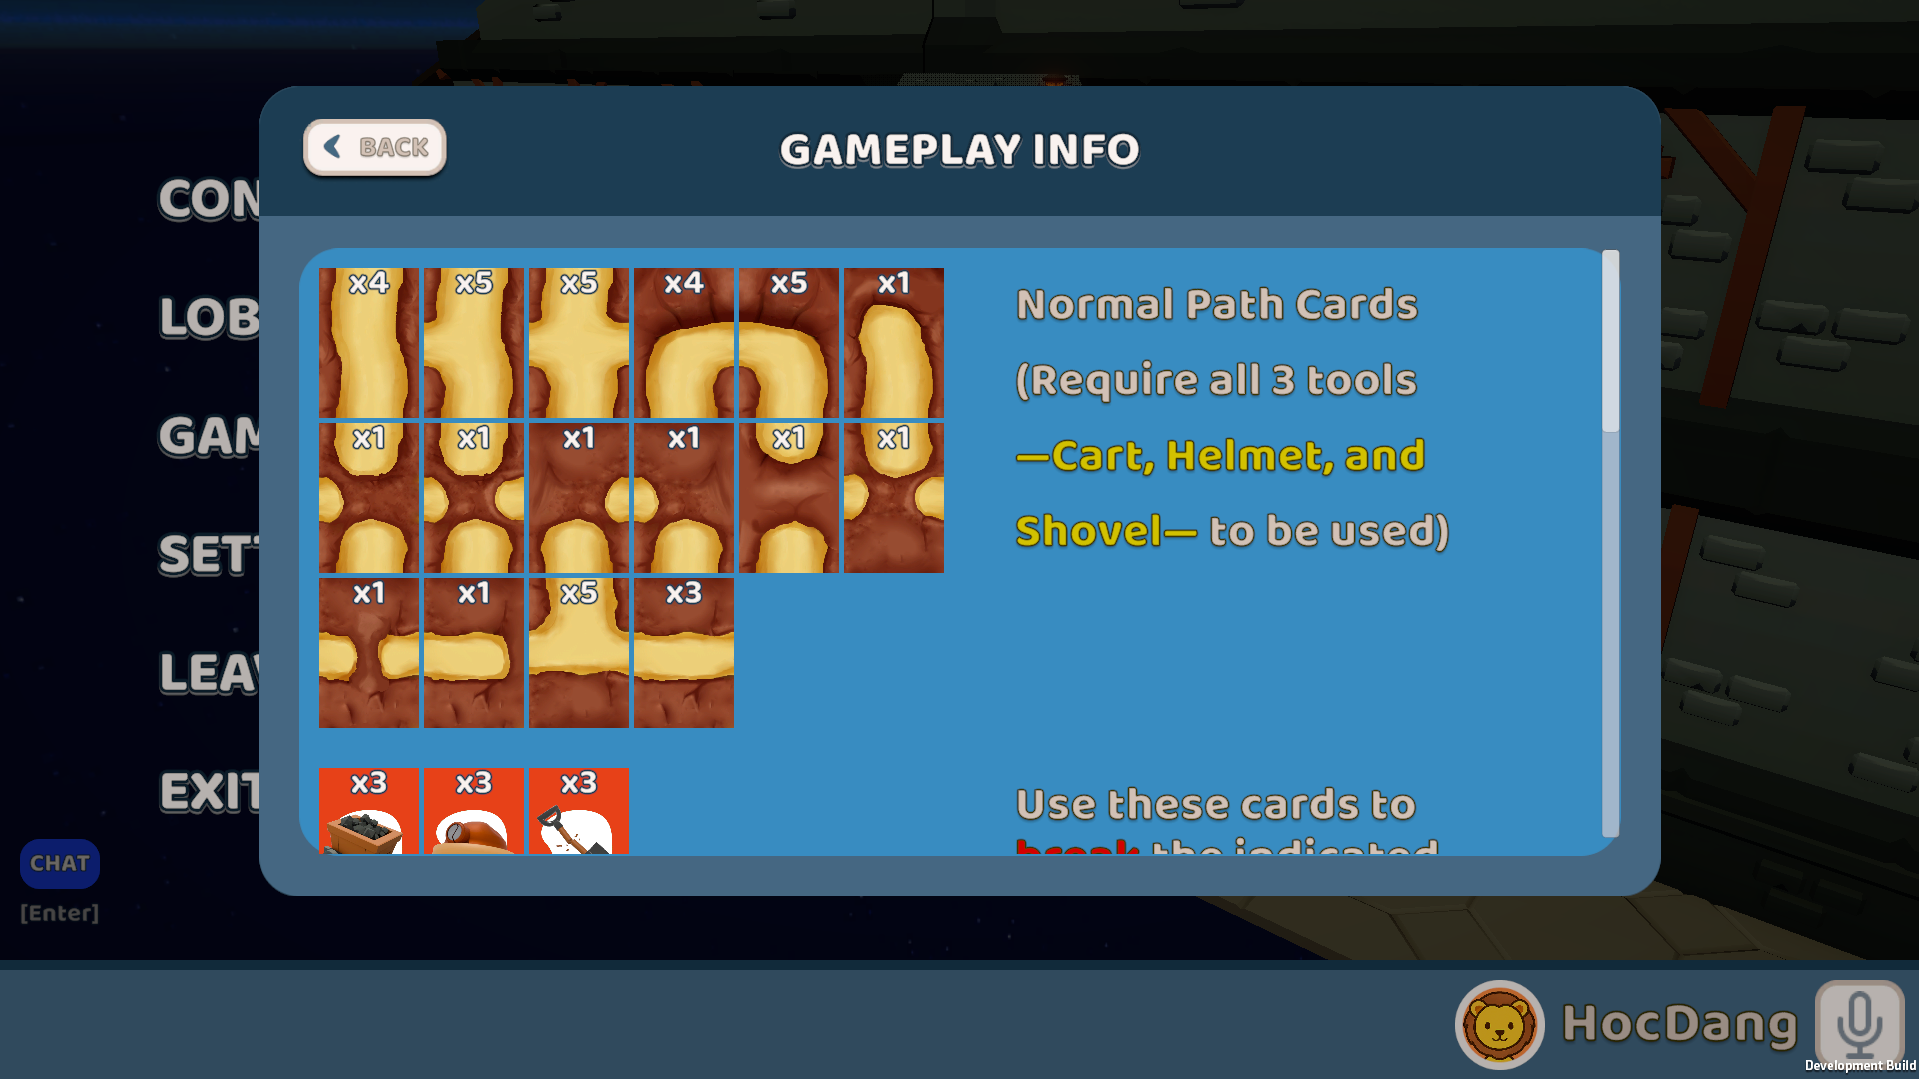
\includegraphics[width=0.75\linewidth]{10.Kết quả/images/PlayGameInfo.png}
    \caption{Screenshot màn hình Gameplay Info của trò chơi}
    \label{fig:placeholder}
\end{figure}

\subsection{Cơ chế chính của trò chơi}
\subsubsection{Cơ chế chọn thẻ bài}
Khi đến lượt của người chơi, người chơi có thể di chuột vào thẻ bài để có thể chọn thẻ bài mình muốn sử dụng, nếu thẻ đó có thể sử dụng được thì sẽ có viền màu vàng và di chuyển lên trên, còn nếu không sử dụng được thì sẽ có viền màu đỏ và đứng im không di chuyển.
\begin{figure} [H]
    \centering
    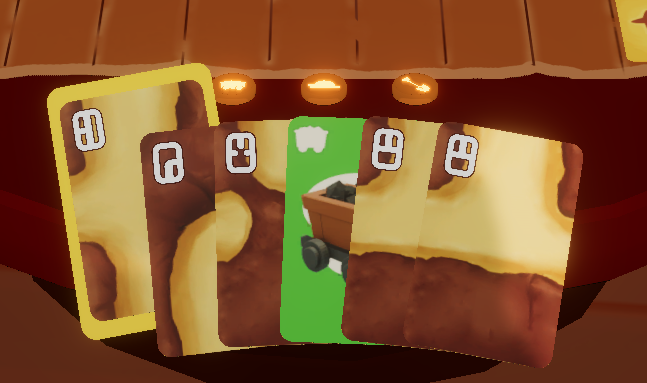
\includegraphics[width=0.5\linewidth]{10.Kết quả//images/SelectCard.png}
    \caption{Screenshot chọn thẻ bài dùng được}
    \label{fig:placeholder}
\end{figure}
\begin{figure}[H]
    \centering
    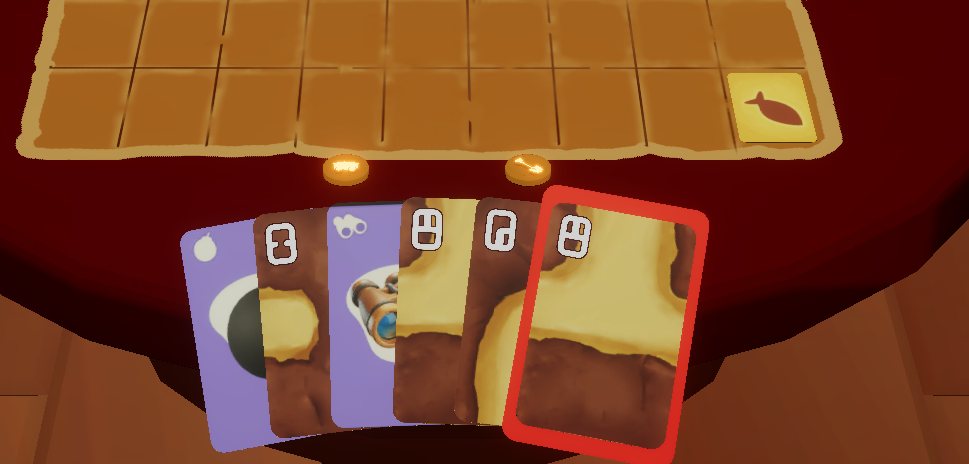
\includegraphics[width=0.5\linewidth]{10.Kết quả//images/CannotHoverCard.png}
    \caption{Screenshot chọn thẻ bài không dùng được}
    \label{fig:placeholder}
\end{figure}
Khi nhấn vào sử dụng thẻ bài nào thì thẻ bài đó sẽ di chuyển xuống dưới bàn và hiển thị những vị trí có thể đặt được, người chơi chỉ cần di chuyển chuột đến vị trí đó rồi nhấn chuột trái là có thể sử dụng. Ở đây chia ra làm 4 loại thẻ bài:
\begin{itemize}
    \item \textbf{Thẻ đường} sẽ đặt lên những vị trí có thể đặt dựa trên trạng thái board hiện tại và đường đi của thẻ.
    \item \textbf{Thẻ hành động} như phá, hồi phục công cụ, dùng khiên thì sẽ cần phải di chuột vào người chơi.
    \item \textbf{Thẻ liên quan đến kho báu} như xem thẻ kho báu, đổi vị trí kho báu thì cần di chuột vào 1 trong 3 thẻ kho báu ở trên bàn.
    \item Riêng \textbf{Thẻ hành động đặt bom} thì cần phải di chuột vào những thẻ đường đã được đặt xuống trừ thẻ bắt đầu và thẻ kho báu.
\end{itemize}    
\begin{figure} [H]
    \centering
    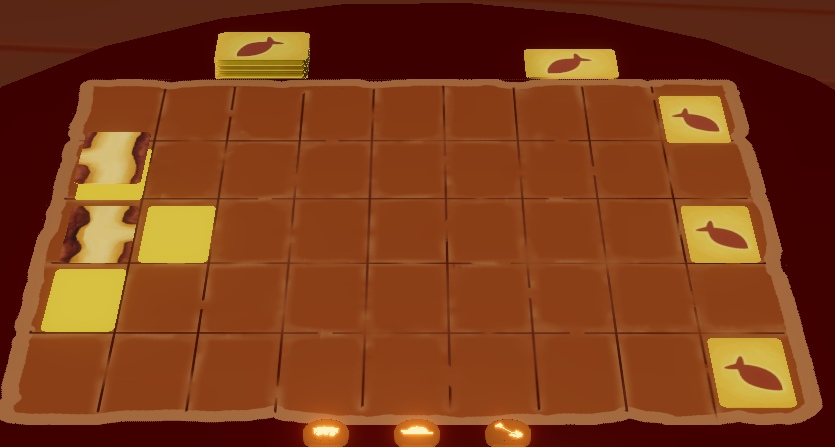
\includegraphics[width=0.5\linewidth]{10.Kết quả//images/PlaceCard.png}
    \caption{Screenshot đặt card xuống}
\end{figure}
\begin{figure}[H]
    \centering
    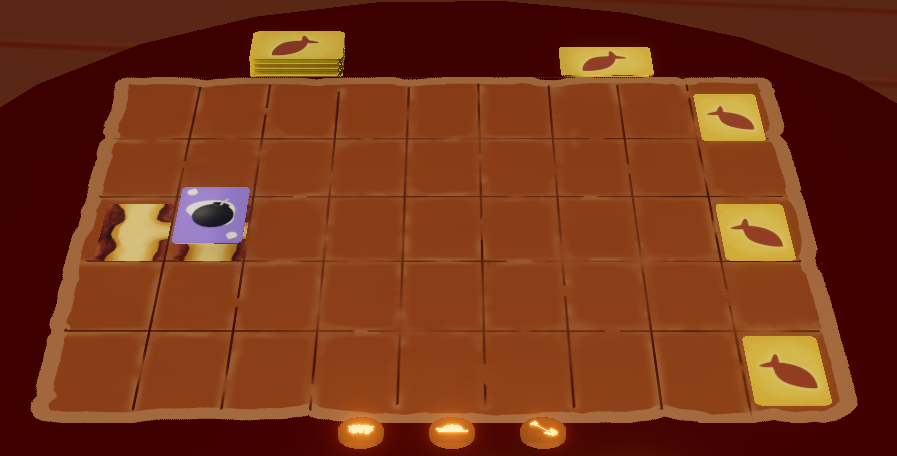
\includegraphics[width=0.5\linewidth]{10.Kết quả//images/HoverBomb.png}
    \caption{Screenshot chọn vị trí đặt bom}
    \label{fig:placeholder}
\end{figure}
\begin{figure}[H]
    \centering
    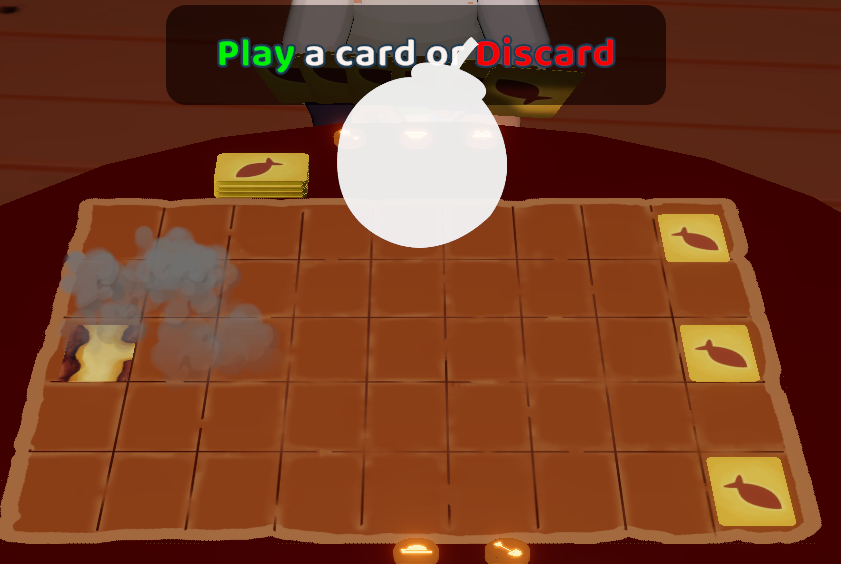
\includegraphics[width=0.5\linewidth]{10.Kết quả//images/BombUsed.png}
    \caption{Screenshot sử dụng bom}
    \label{fig:placeholder}
\end{figure}
\begin{figure}[H]
    \centering
    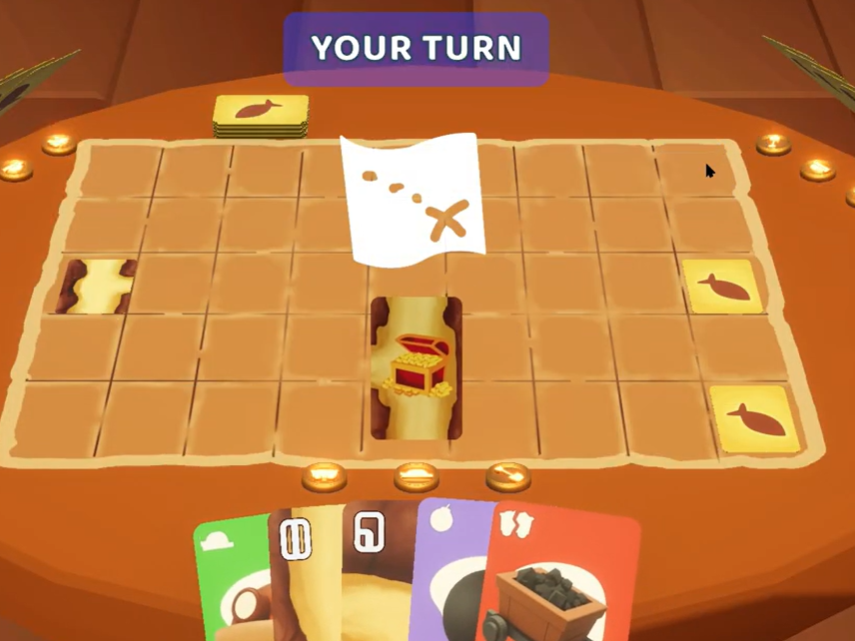
\includegraphics[width=0.5\linewidth]{10.Kết quả//images/MapUsed.png}
    \caption{Screenshot sử dụng thẻ xem kho báu}
    \label{fig:placeholder}
\end{figure}
\begin{figure}[H]
    \centering
    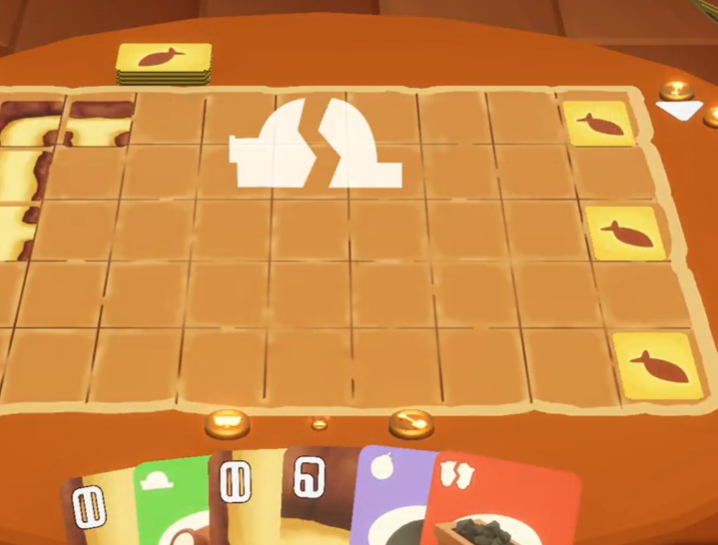
\includegraphics[width=0.5\linewidth]{10.Kết quả//images/BreakTool.png}
    \caption{Screenshot sử dụng thẻ phá công cụ}
    \label{fig:placeholder}
\end{figure}
\begin{figure}[H]
    \centering
    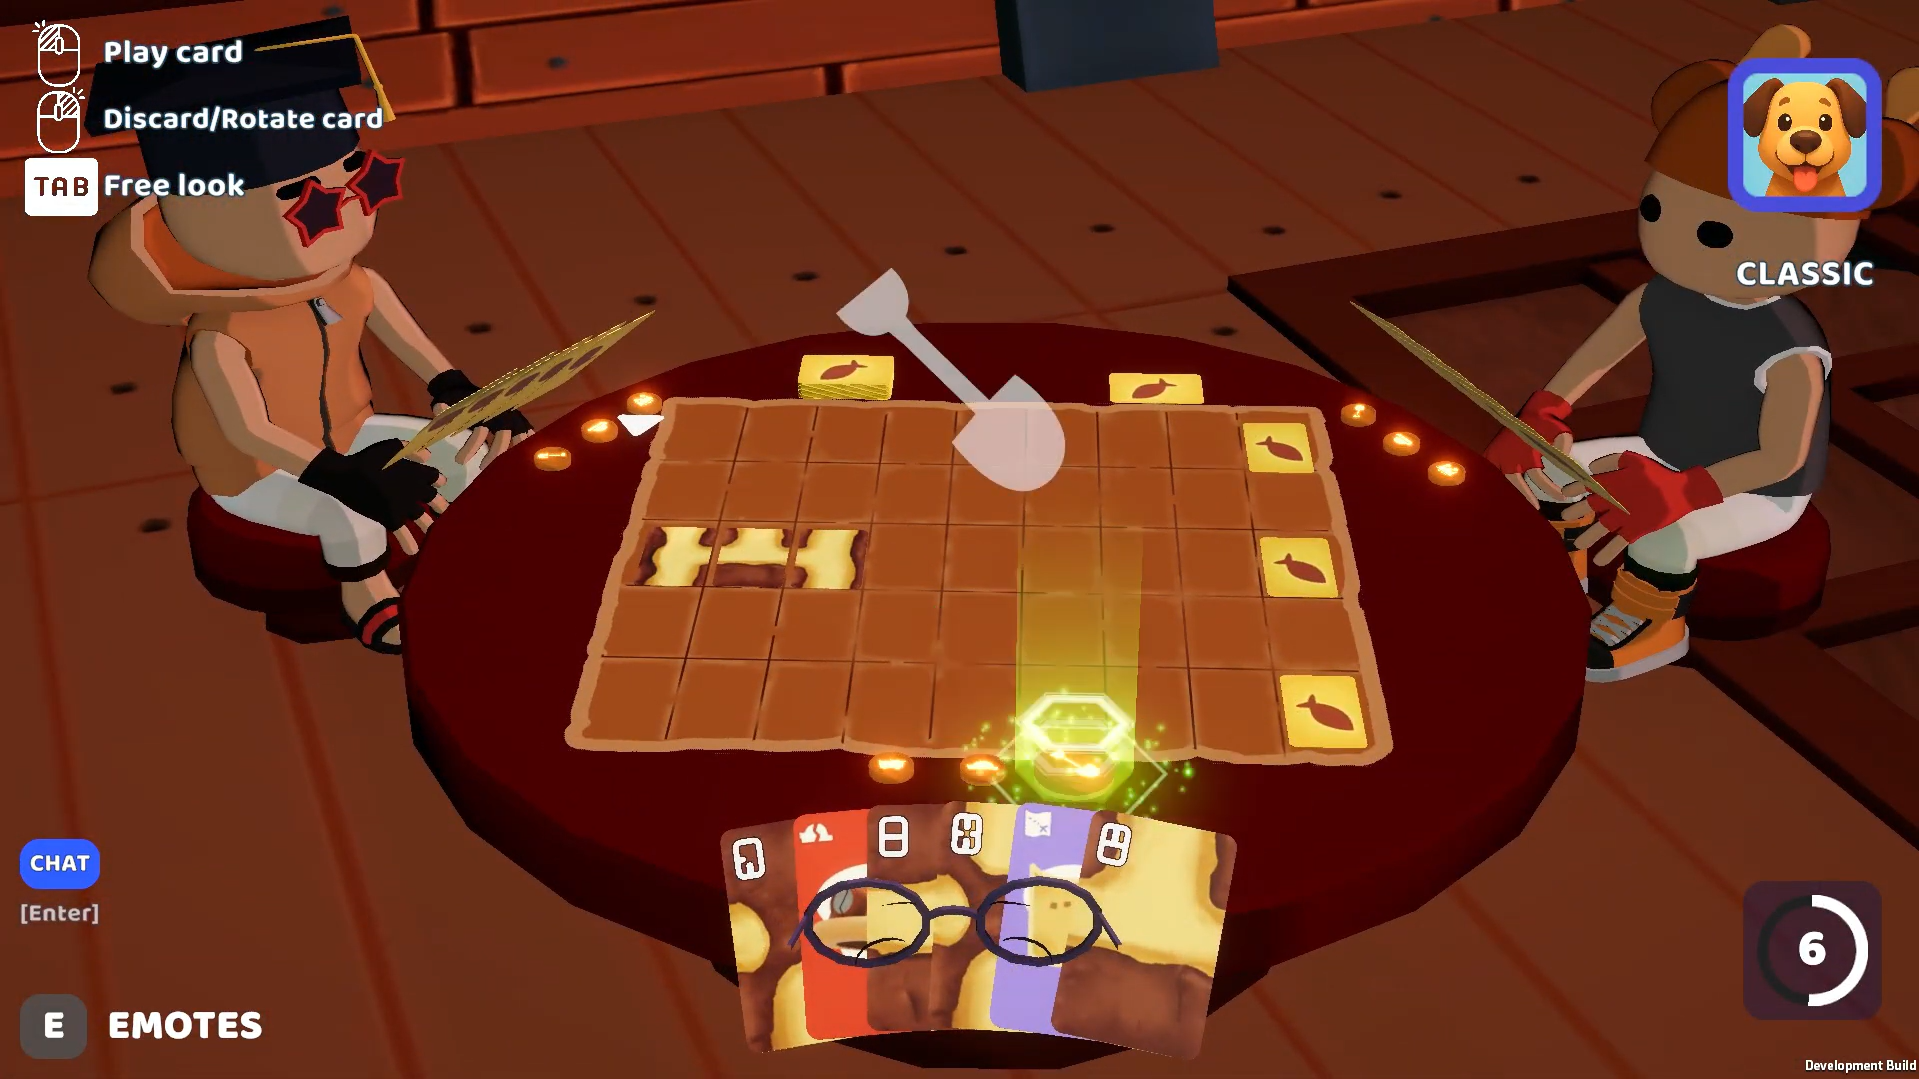
\includegraphics[width=0.5\linewidth]{10.Kết quả//images/ReviveTool.png}
    \caption{Screenshot sử dụng thẻ chức năng hồi phục công cụ}
    \label{fig:placeholder}
\end{figure}

\begin{figure}[H]
    \centering
    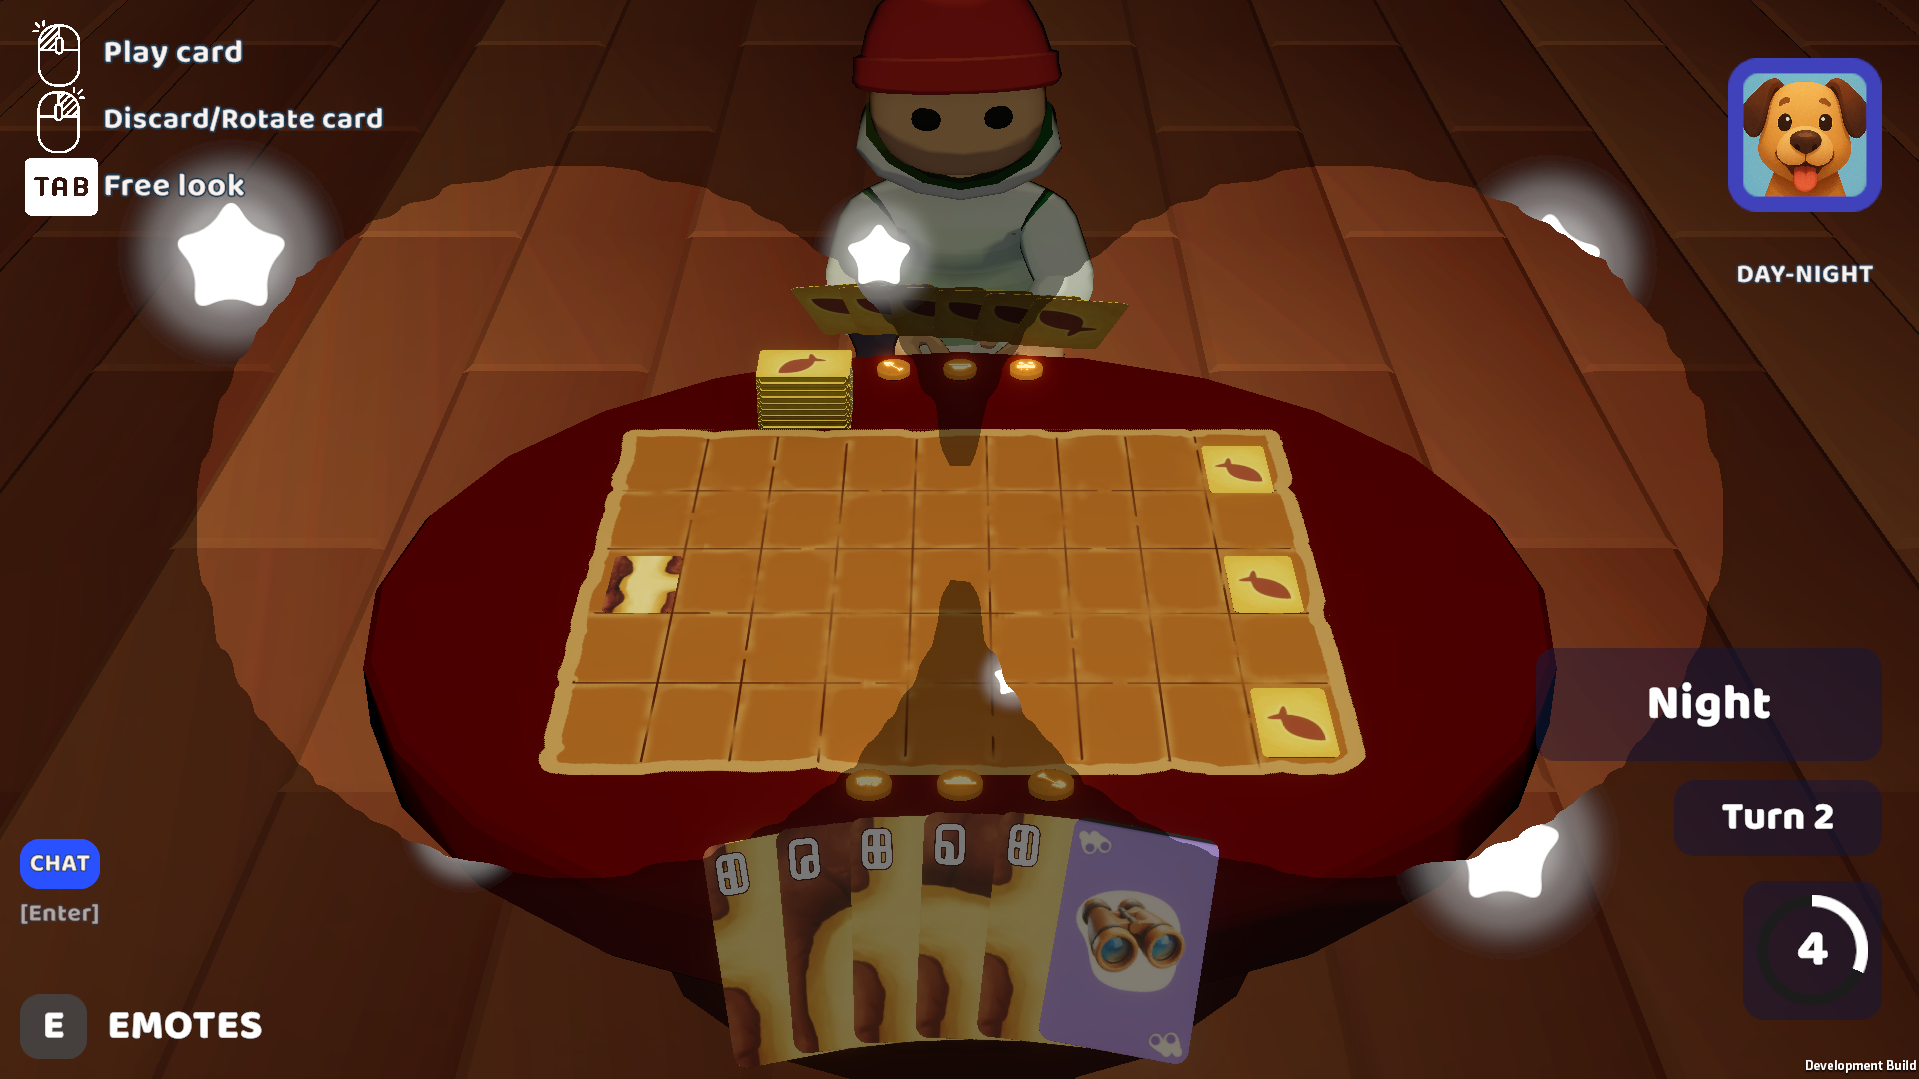
\includegraphics[width=0.5\linewidth]{10.Kết quả//images/Binocular.png}
    \caption{Screenshot sử dụng thẻ chức năng binoculars}
    \label{fig:placeholder}
\end{figure}

Sau khi đặt các thẻ đường sao cho có đường đến kho báu hoặc không còn thẻ bài nào trong tay bất kỳ người chơi nào thì sẽ kết thúc game đấu.
\begin{figure}[H]
    \centering
    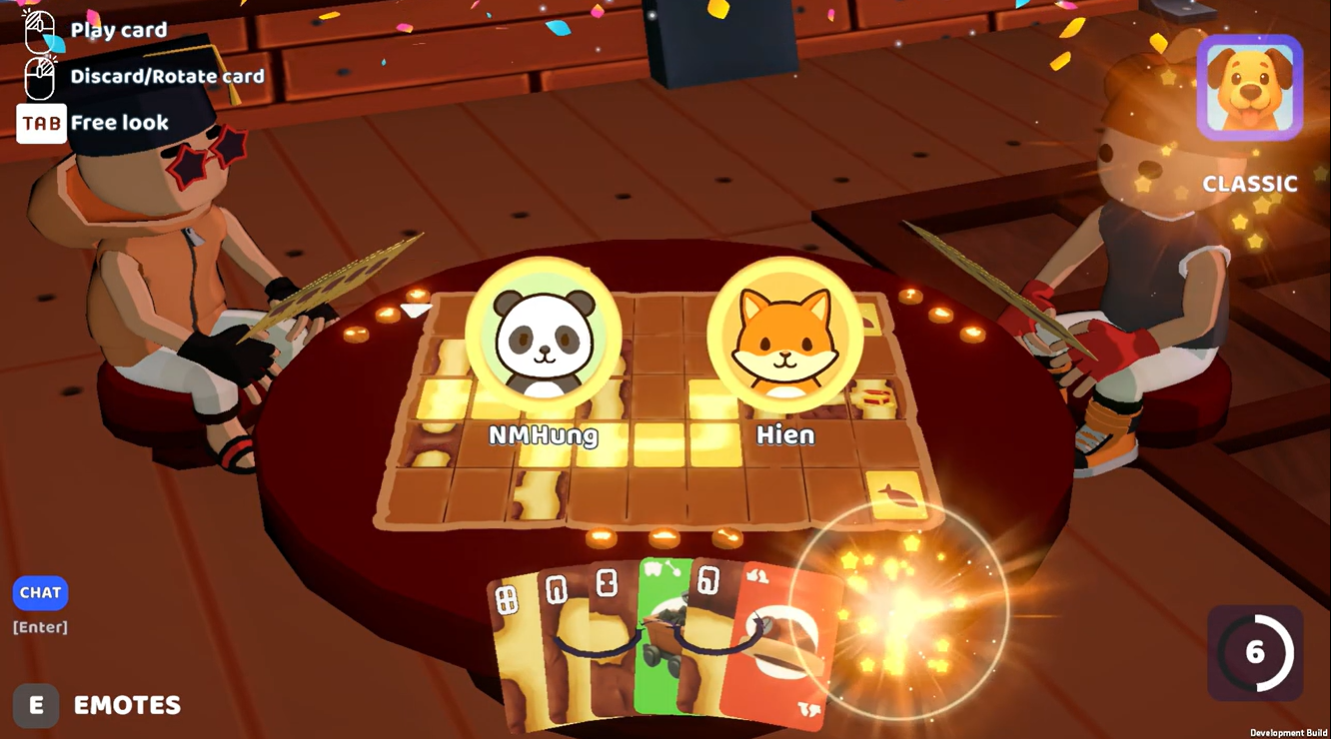
\includegraphics[width=0.5\linewidth]{10.Kết quả//images/victory.png}
    \caption{Screenshot màn hình \textbf{Chiến thắng}}
    \label{fig:placeholder}
\end{figure}
\subsection{Các hệ thống khác của trò chơi}
\subsubsection{Hệ thống cài đặt}
Giao diện cài đặt của trò chơi được hiển thị khi người chơi nhấn vào nút cài đặt, cửa sổ giao diện cài đặt gồm các thông tin như hình dưới:
\begin{figure}[H]
    \centering
    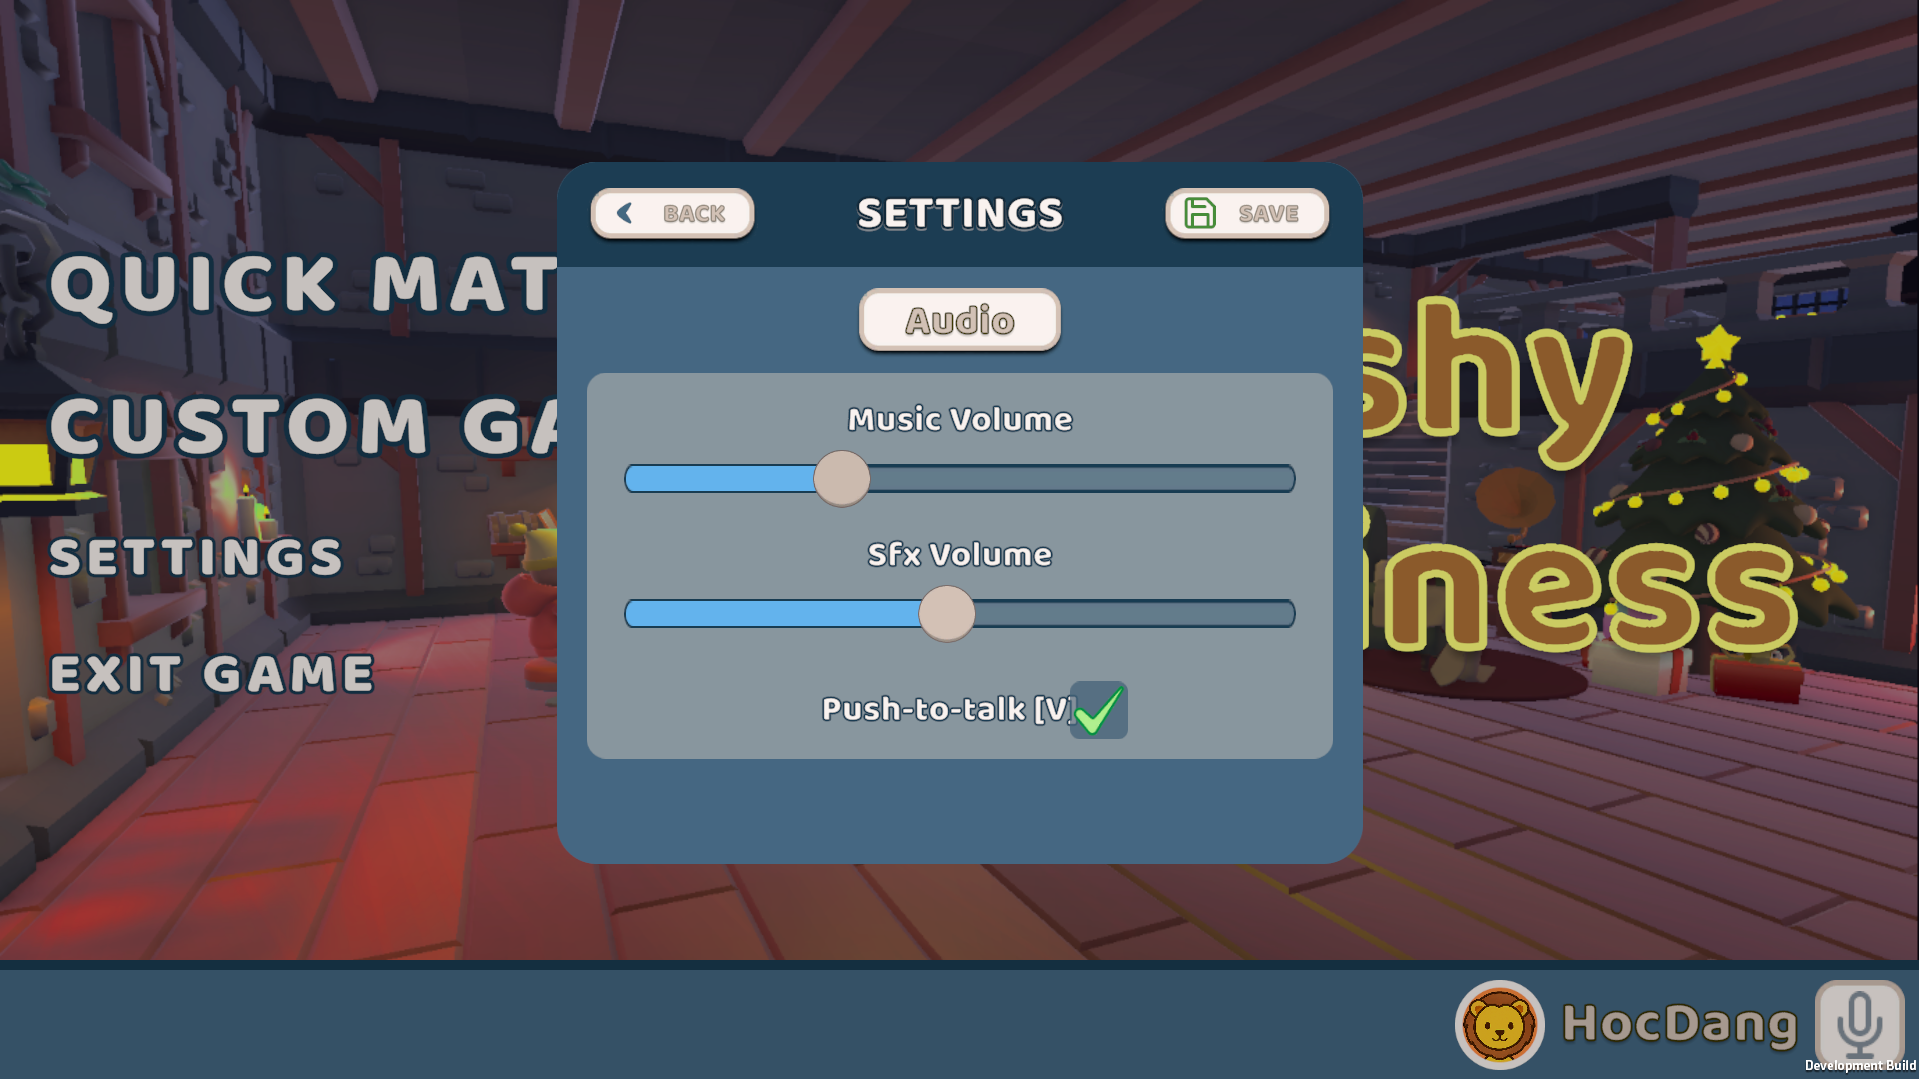
\includegraphics[width=0.75\linewidth]{10.Kết quả/images/Setting.png}
    \caption{Screenshot giao diện cài đặt của trò chơi}
    \label{fig:game-object}
\end{figure}
\begin{itemize}
    \item \textbf{Music Volume}: điều chỉnh âm lượng của nhạc nền
    \item \textbf{Sfx Volume}: điều chỉnh âm lượng của các hiệu ứng âm thanh
    \item \textbf{Push to talk}: tắt/bật chế độ cần phải nhấn giữ nút \textbf{''V''} để nói.
\end{itemize}
\subsubsection{Hệ thống Tooltip}
Khi bạn đang chơi game mà không biết chế độ, vai trò của bạn là gì thì có thể để chuột vào icon, dòng chữ đó để có thể hiện ra \textbf{tooltip}.
\begin{figure}[H]
    \centering
    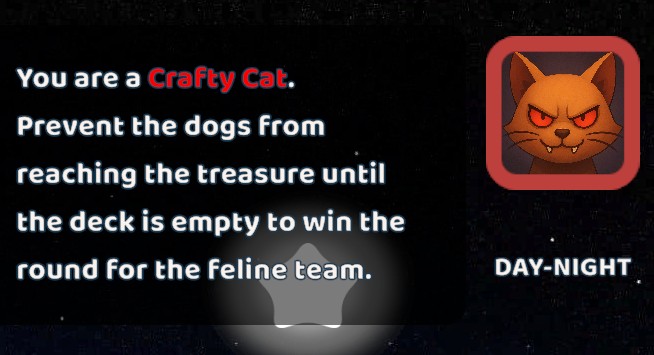
\includegraphics[width=0.75\linewidth]{10.Kết quả/images/CatTooltip.png}
    \caption{Screenshot Tooltip vai trò mèo của trò chơi}
    \label{fig:game-object}
\end{figure}
\begin{figure}[H]
    \centering
    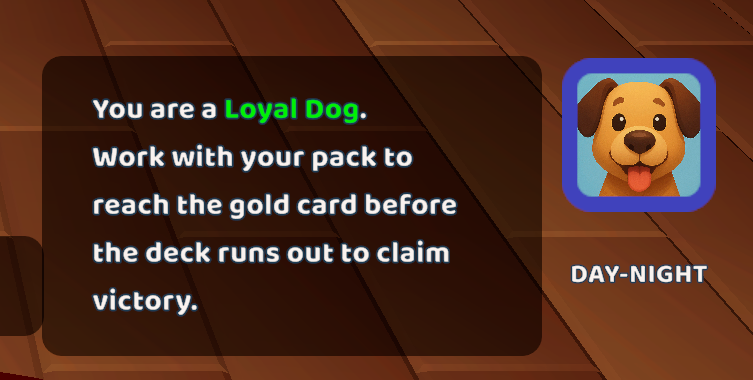
\includegraphics[width=0.75\linewidth]{10.Kết quả/images/DogTooltip.png}
    \caption{Screenshot Tooltip vai trò chó của trò chơi}
    \label{fig:game-object}
\end{figure}
\begin{figure}[H]
    \centering
    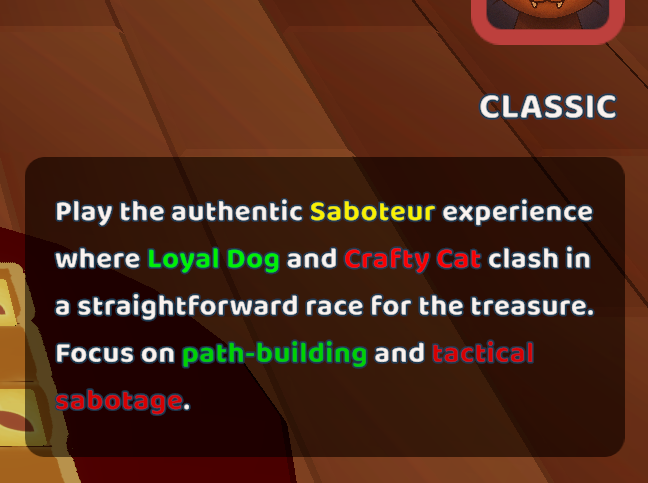
\includegraphics[width=0.75\linewidth]{10.Kết quả/images/ClassicTooltip.png}
    \caption{Screenshot Tooltip chế độ classic của trò chơi}
    \label{fig:game-object}
\end{figure}
\begin{figure}[H]
    \centering
    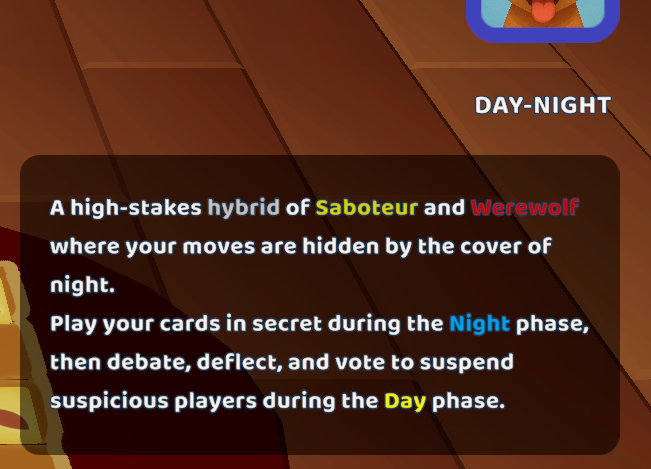
\includegraphics[width=0.75\linewidth]{10.Kết quả/images/DayNightTooltip.png}
    \caption{Screenshot Tooltip chế độ Day Night của trò chơi}
    \label{fig:game-object}
\end{figure}

\subsubsection{Hoạt động ngoài lề}
Người chơi cũng có thể đứng trước gương và nhấn giữ \textbf{''F''} để vào trạng thái thay trang phục, sau khi chọn xong trang phục mình muốn, người chơi có thể nhấn giữ phím \textbf{''F''} để thoát:
\begin{figure}[H]
    \centering
    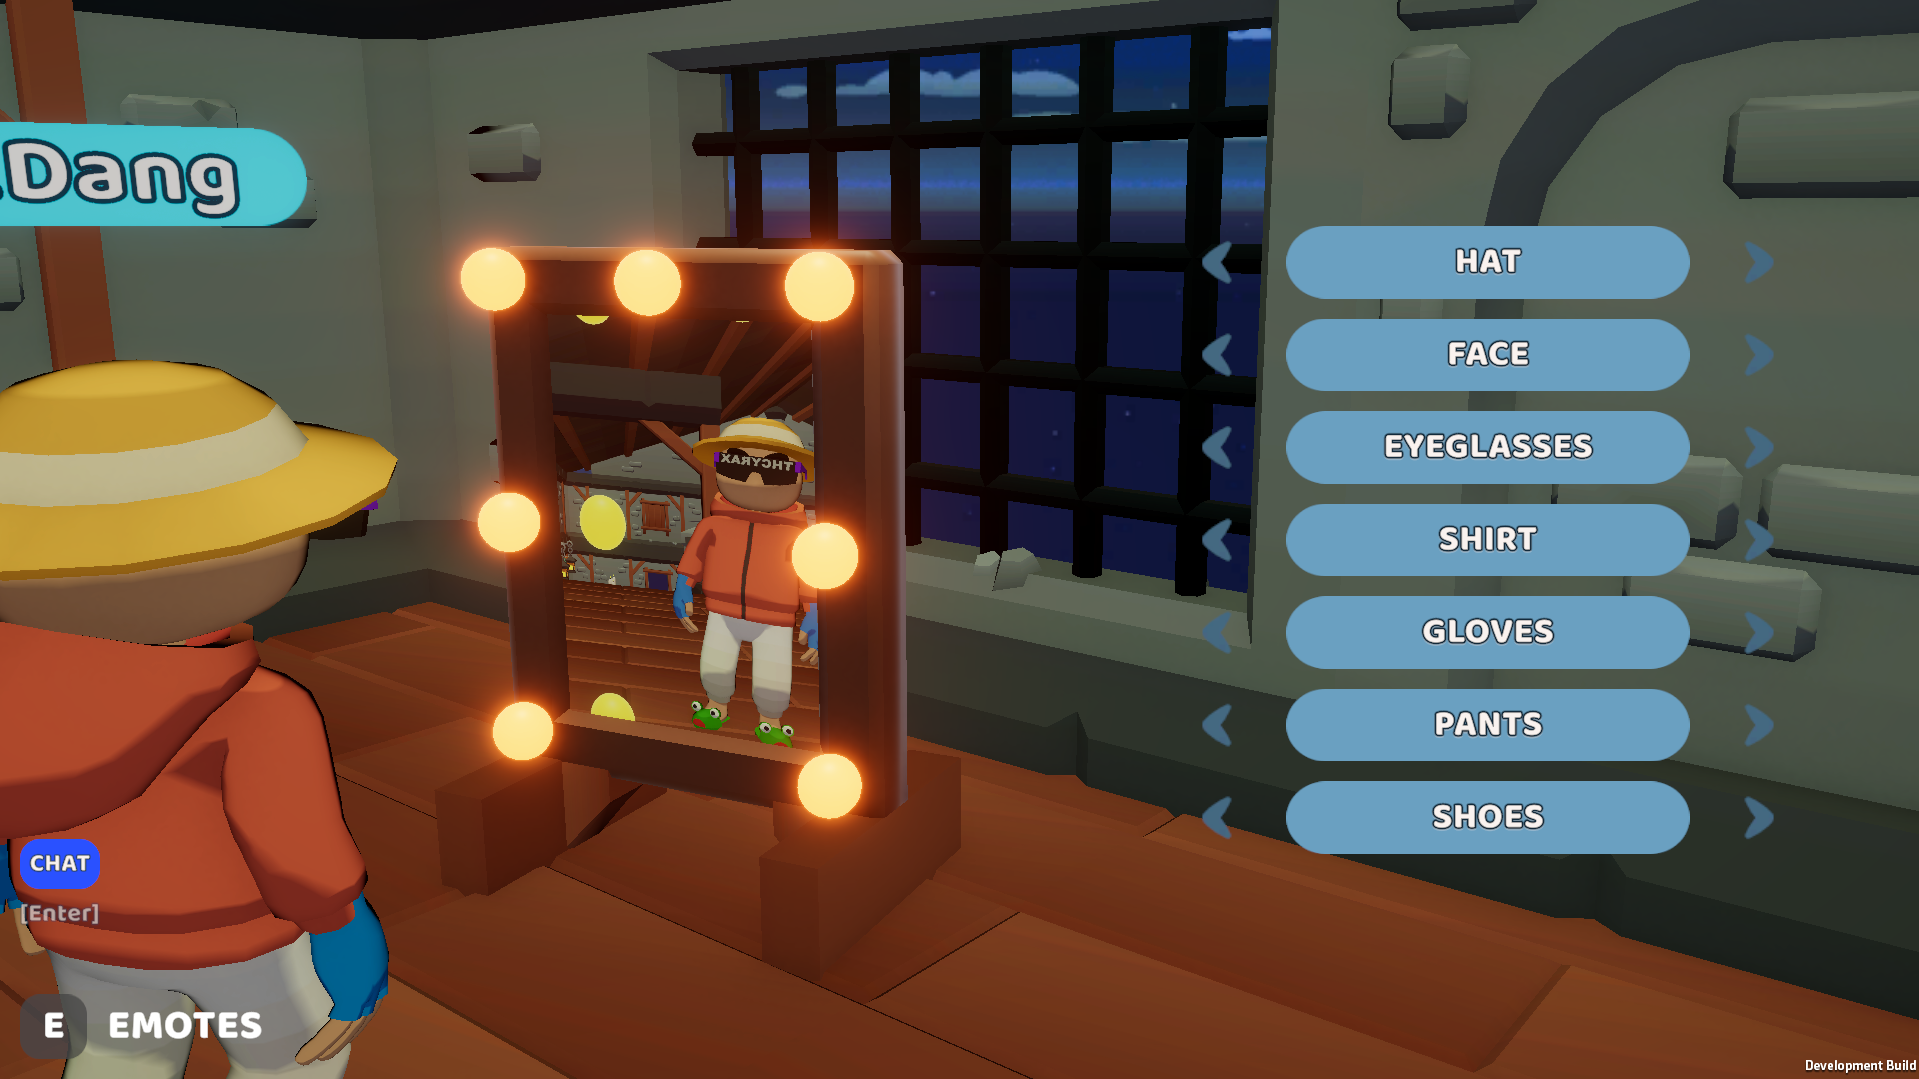
\includegraphics[width=0.75\linewidth]{10.Kết quả/images/ChangeSkin.png}
    \caption{Screenshot màn hình chọn trang phục của trò chơi}
    \label{fig:game-object}
\end{figure}
Hoặc người chơi cũng có thể đến chiếc ghế trước piano và nhấn giữ phím \textbf{''F''} để có thể ngồi vào. Tại đây người chơi có thể bắt đầu tương tác với piano bằng cách nhấn 7 phím đầu tiên của 3 hàng chữ trên bàn phím.
\begin{figure}[H]
    \centering
    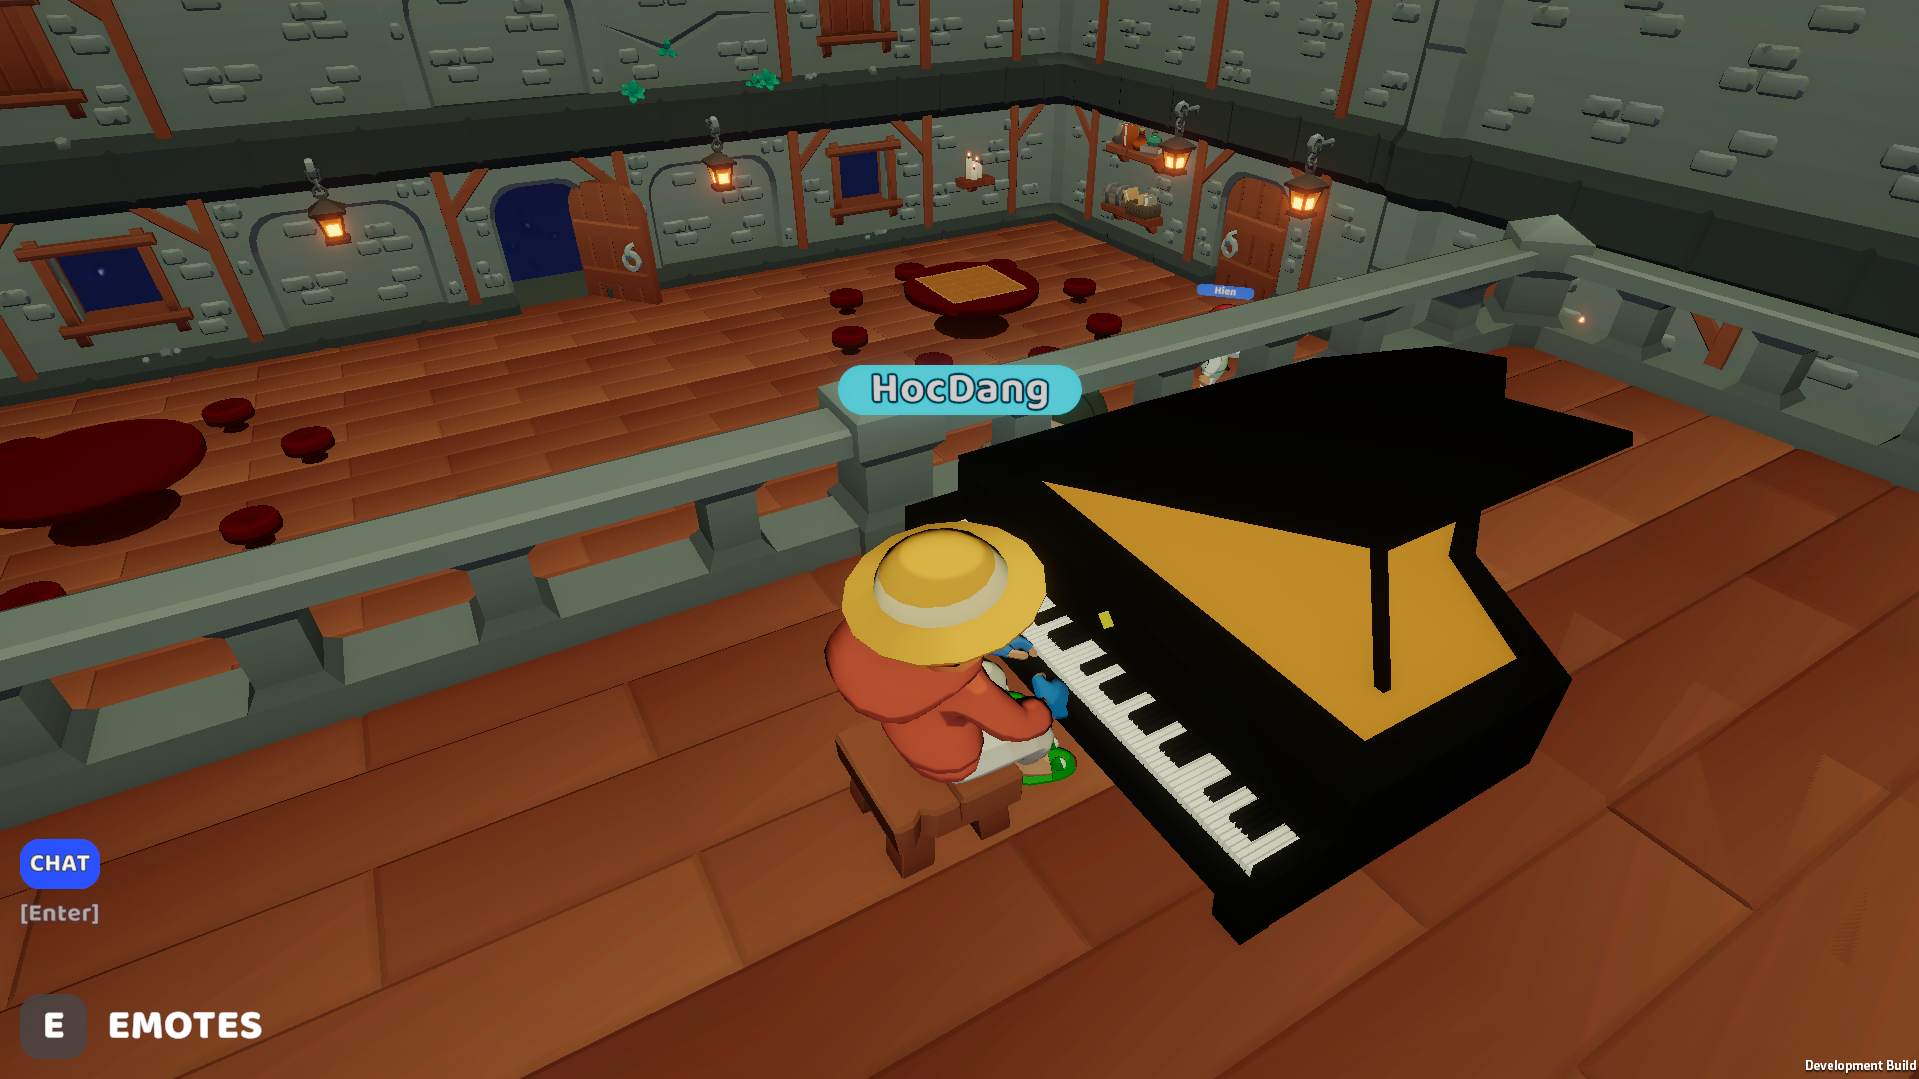
\includegraphics[width=0.75\linewidth]{10.Kết quả/images/PlayPiano.png}
    \caption{Screenshot màn hình chơi piano của trò chơi}
    \label{fig:game-object}
\end{figure}

Hơn nữa người chơi cũng có thể nhấn giữ phím \textbf{''E''} và sử dụng \textbf{lăn chuột} để chọn 1 emote để nhấn vật của người chơi có thể thực hiện một hành động như là nhảy, vẫy tay, ...
\begin{figure}[H]
    \centering
    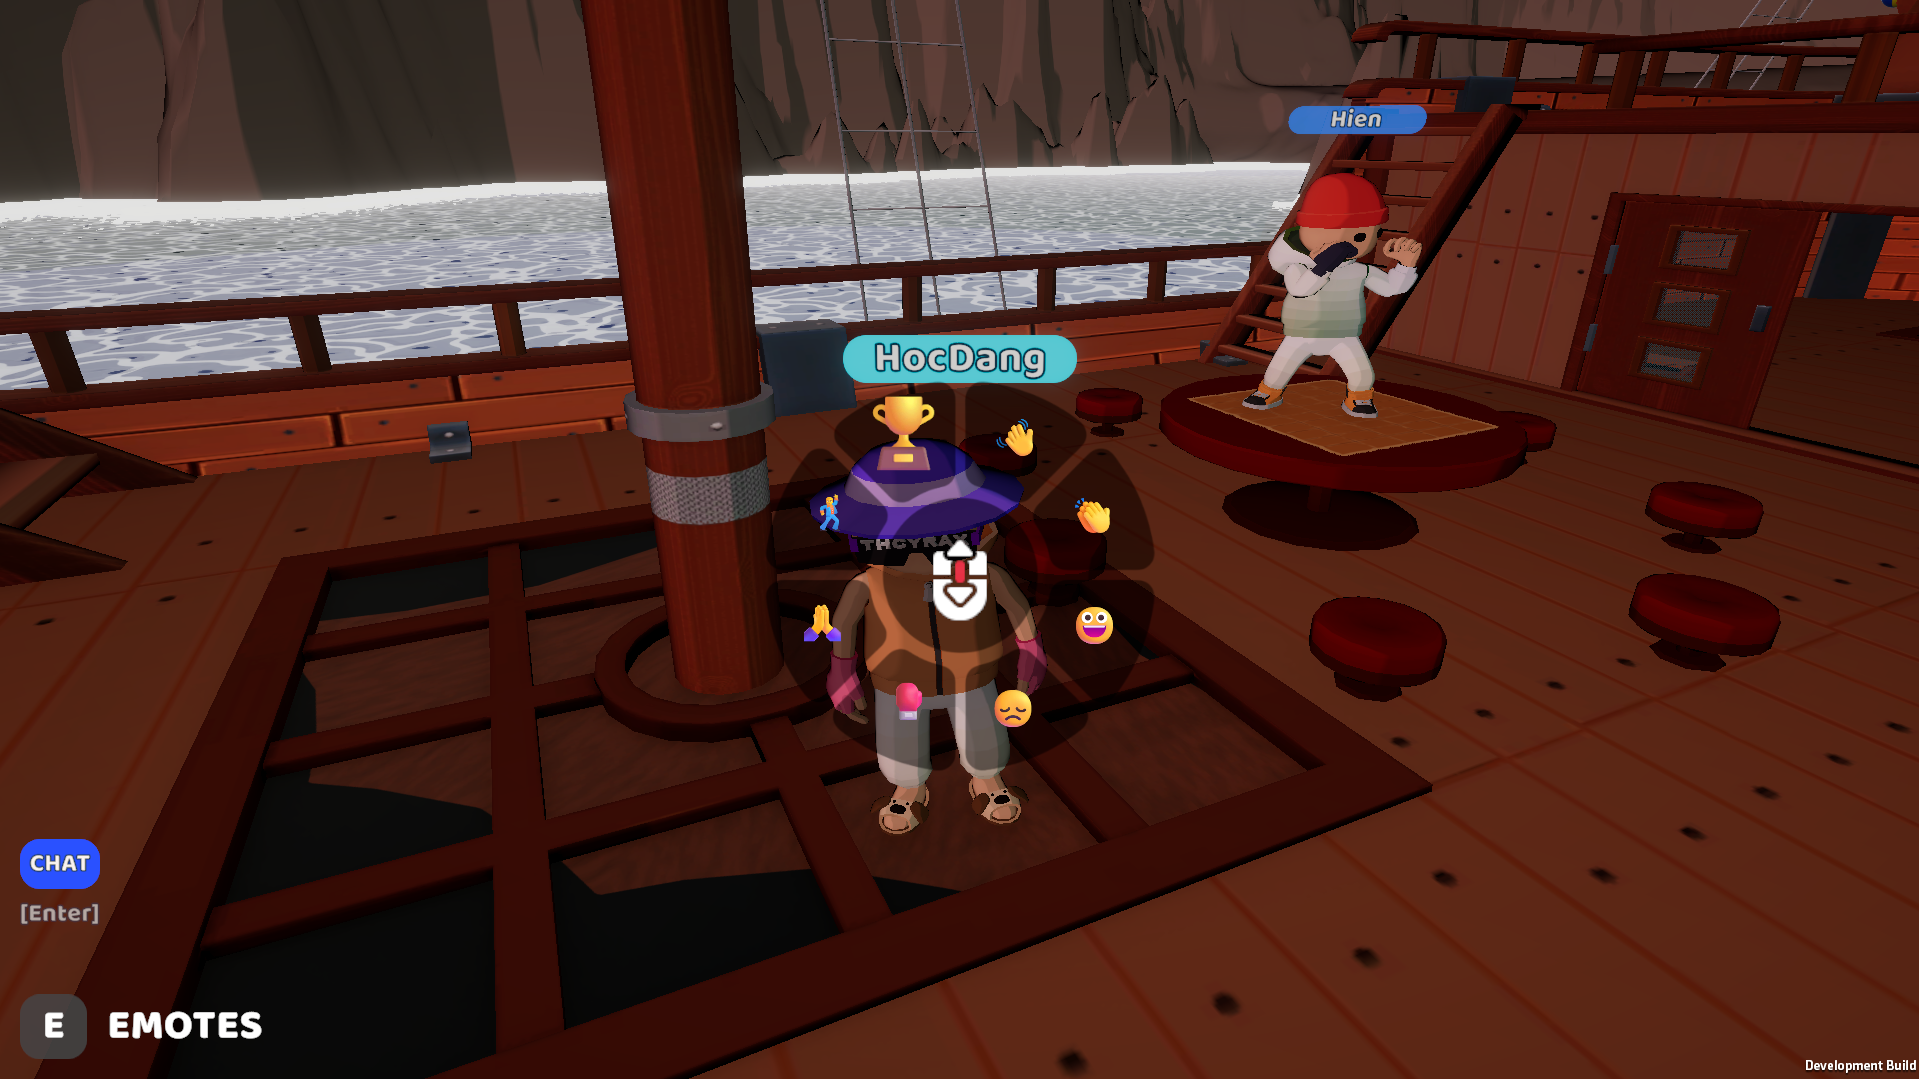
\includegraphics[width=0.75\linewidth]{10.Kết quả/images/Emote.png}
    \caption{Screenshot màn hình Emotes của trò chơi}
    \label{fig:game-object}
\end{figure}

Người chơi cũng có thể nhấn phím \textbf{''Enter''} để mở hộp thoại text chat và bắt đầu chat với những người chơi khác:
\begin{figure} [H]
    \centering
    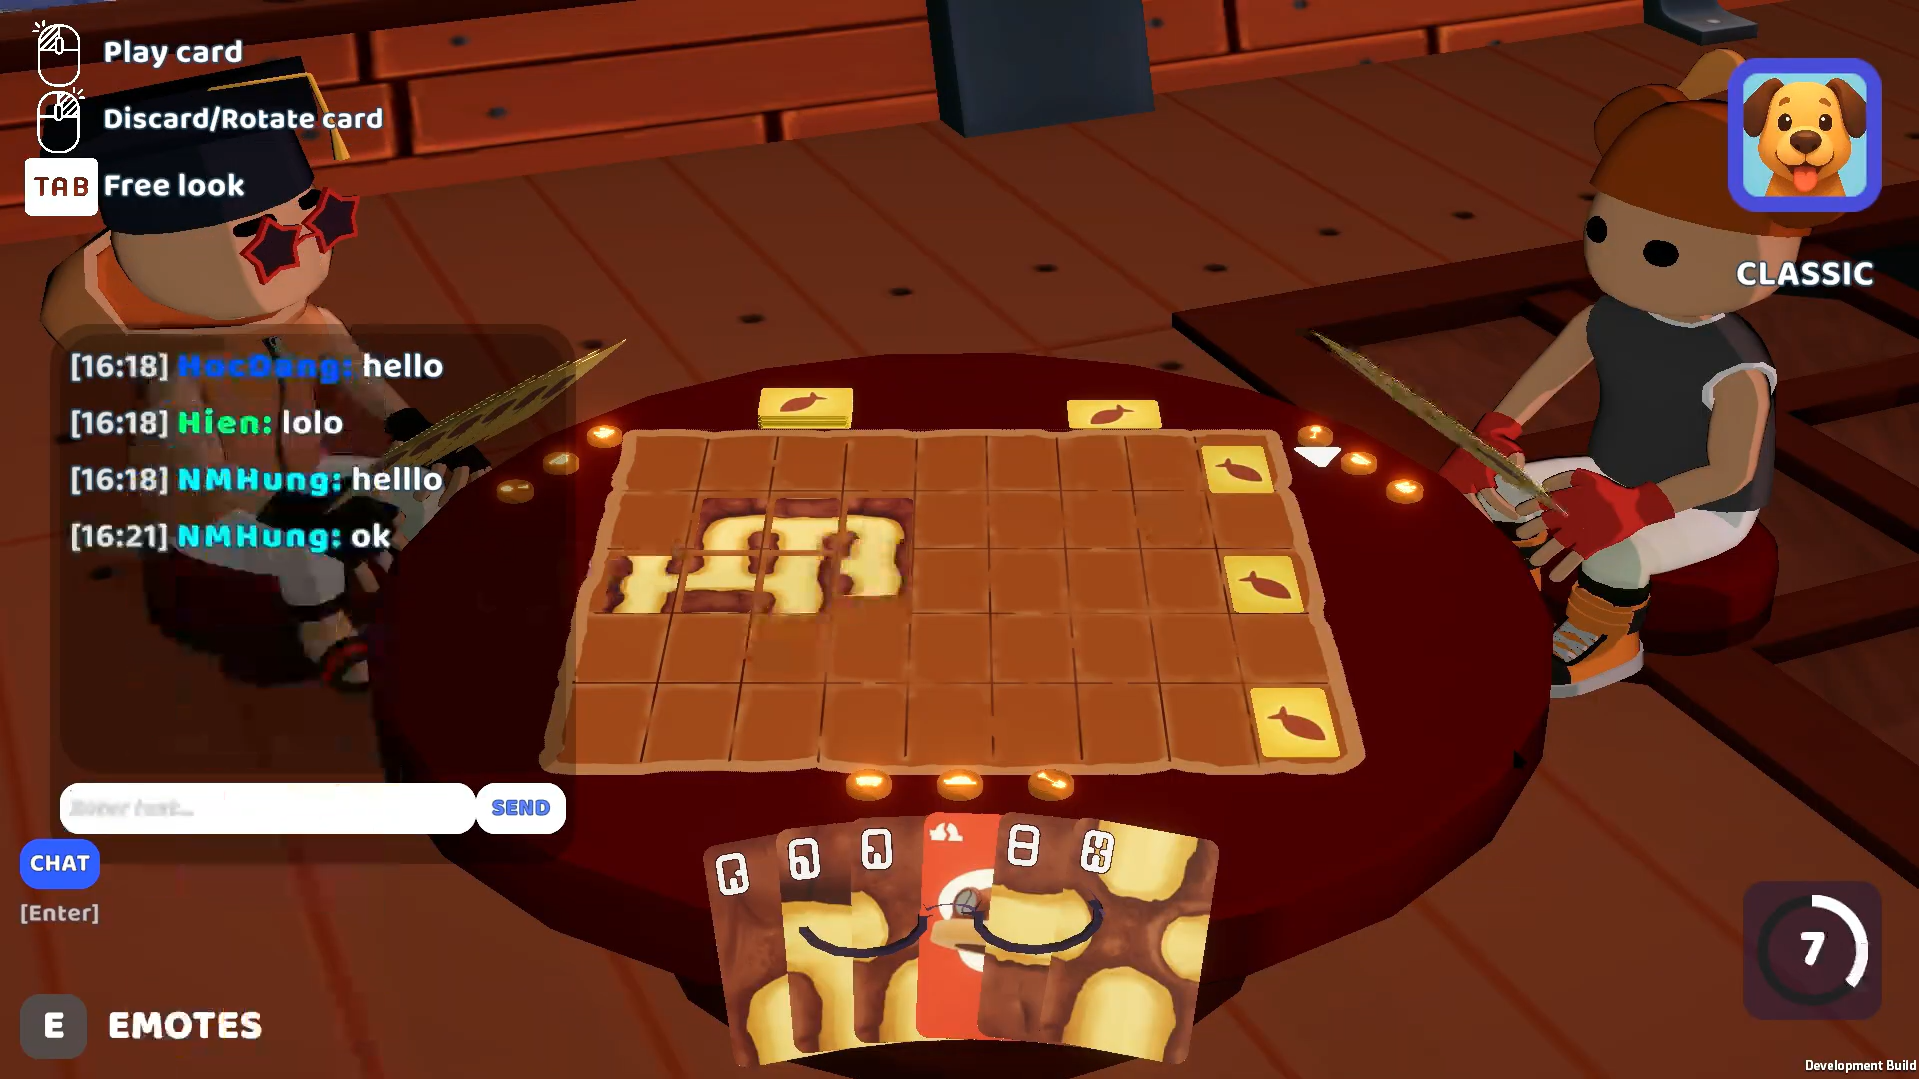
\includegraphics[width=0.75\linewidth]{10.Kết quả/images/TextChat.png}
    \caption{Screenshot màn hình text chat của trò chơi}
    \label{fig:placeholder}
\end{figure}

\section{Thu thập dữ liệu người dùng và đánh giá}

Để đánh giá chất lượng trò chơi \textit{Fishy Business} một cách khách quan và thu thập ý kiến phản hồi trực tiếp từ người chơi, nhóm đã tiến hành khảo sát trải nghiệm game thông qua Google Forms. Khảo sát được thiết kế nhằm đo lường mức độ hài lòng của người dùng đối với các yếu tố cốt lõi như cơ chế gameplay, giao diện, hiệu năng multiplayer, âm thanh – hình ảnh, cũng như các tính năng ngoài lề (emotes, voice chat, piano, thay trang phục). 

Form khảo sát: \href{https://forms.gle/mCoSvJsexBnodXNa7}{có tại đây}

Kết quả khảo sát:
\href{https://docs.google.com/spreadsheets/d/1KZl3N0H3yh3VPaNN1_ZQd04tOZtS0NndB_7dkX4CN0o/edit?usp=sharing}{có tại đây}

Tính đến thời điểm hoàn thành báo cáo, khảo sát đã thu thập được \textbf{9 phản hồi} từ người chơi (toàn bộ thuộc độ tuổi 18--24). 

Điểm số tổng thể mà người chơi chấm cho đồ án là:
\begin{itemize}
    \item Điểm cao nhất: 10/10 (3 người)
    \item Điểm thấp nhất: 7/10 (1 người)
    \item \textbf{Điểm trung bình: 9.0/10}
\end{itemize}

Xu hướng chung cho thấy người chơi đánh giá rất cao chất lượng trò chơi:
\begin{itemize}
    \item \textbf{Đồ họa tổng quan, nhân vật 3D, thẻ bài \& board}: hầu hết đạt 4--5/5.
    \item \textbf{Giao diện UI, hiệu ứng âm thanh, nhạc nền}: 4--5/5 (chỉ một số ít đánh giá 3).
    \item \textbf{Độ mượt mà điều khiển nhân vật, camera, chọn thẻ bài}: trung bình 4/5.
    \item \textbf{Gameplay}: 
        \begin{itemize}
            \item Classic mode: trung bình 4.3/5
            \item Day-Night mode: trung bình 4.2/5
        \end{itemize}
    \item \textbf{Multiplayer \& Networking}: phần lớn đánh giá 4--5/5, một số góp ý nhỏ về độ lag và hiện tượng teleport.
\end{itemize}

Các yếu tố được người chơi ấn tượng nhất (trích dẫn nguyên văn một số phản hồi tiêu biểu):
\begin{itemize}
    \item ``Gameplay thú vị, nhạc hay''
    \item ``Gameplay khá mới lạ''
    \item ``Multiplayer''
    \item ``Đồ họa đẹp''
    \item ``Nhóm làm game multiplayer có vẻ mạnh''
    \item ``Game tương tác với nhau vui''
\end{itemize}

Về góp ý cải thiện và bug tồn đọng, người chơi đề xuất:
\begin{itemize}
    \item Giảm độ lag, tối ưu hiệu năng (đặc biệt khi có nhiều người chơi).
    \item Cải thiện độ mượt của animation nhân vật và camera.
    \item Fix lỗi spawn sai vị trí, lỗi khi người chơi thoát trận/đứng mạng.
    \item Thêm effect hình ảnh (VFX) để game bắt mắt hơn.
    \item Thêm nhiều bản đồ, thẻ bài chức năng và tính năng mới.
    \item Nâng cấp thêm tooltip và hướng dẫn cho người mới.
\end{itemize}

Tỷ lệ người chơi sẵn sàng chơi bản chính thức sau này:
\begin{itemize}
    \item \textbf{Chắc chắn có}: 5 người (55.6\%)
    \item \textbf{Có thể}: 4 người (44.4\%)
    \item Không có phản hồi tiêu cực.
\end{itemize}

Tổng thể, kết quả khảo sát khẳng định \textit{Fishy Business} đã đạt được mục tiêu cốt lõi: mang lại trải nghiệm giải trí vui vẻ, hấp dẫn khi chơi nhóm, với gameplay sáng tạo và tính tương tác cao. Dữ liệu thu thập sẽ là cơ sở quan trọng để nhóm tiếp tục tối ưu, sửa lỗi và phát triển thêm các tính năng trong tương lai.

\section{Tổng kết}
Dựa vào các phần được trình bày trước đó, nhóm thực hiện đánh giá tổng quan về trò chơi trong phần này, cùng với các công việc đã đóng góp của từng thành viên trong nhóm và kế hoạch tương lai cho trò chơi.
\subsection{Đánh giá chung}
Đến thời điểm hiện tại, dự án Fishy Business đã hoàn thiện được phiên bản release có thể chơi được theo đúng định hướng ban đầu. Để đạt được kết quả này, nhóm đã duy trì được tiến độ ổn định, phối hợp hiệu quả giữa các thành viên và luôn tập trung vào những yếu tố cốt lõi của trò chơi, tránh lan man sang các tính năng chưa cần thiết.

Mục tiêu của dự án là xây dựng một trò chơi board game 3D mang tính giải trí cao, hướng đến trải nghiệm vui vẻ và tương tác giữa các nhóm bạn. Người chơi sẽ điều khiển nhân vật của mình di chuyển trên bàn chơi, tham gia vào các hoạt động cạnh tranh, tương tác và tạo ra những tình huống bất ngờ, thú vị. Trò chơi tập trung vào yếu tố multiplayer, cho phép nhiều người chơi tham gia cùng lúc.

Hiện tại, nhóm đã hoàn thiện các cơ chế chính của trò chơi bao gồm hệ thống di chuyển nhân vật, tương tác trên board, cơ chế chơi nhiều người và đồng bộ dữ liệu giữa các client. Bên cạnh đó, nhiều cải tiến cũng đã được bổ sung so với các phiên bản trước như tối ưu trải nghiệm người chơi, cải thiện độ mượt của gameplay và sửa các lỗi phát sinh trong quá trình phát triển.

Tuy nhiên, dự án vẫn còn đối mặt với một số thách thức cần giải quyết trong thời gian tới. Một trong những vấn đề quan trọng là tối ưu hiệu suất để đảm bảo trò chơi hoạt động ổn định trên nhiều nền tảng khác nhau. Ngoài ra, việc nâng cao chất lượng hệ thống multiplayer, giảm độ trễ và đảm bảo đồng bộ chính xác giữa các người chơi cũng là mục tiêu quan trọng để cải thiện trải nghiệm tổng thể. Việc thu thập và phân tích hành vi người chơi trong tương lai cũng sẽ giúp nhóm điều chỉnh gameplay hợp lý hơn, từ đó nâng cao tính hấp dẫn và giữ chân người chơi lâu dài.

Trong quá trình phát triển, nhóm đã tích lũy được nhiều kinh nghiệm quý báu, từ việc thiết kế gameplay multiplayer, xử lý đồng bộ dữ liệu, cho đến việc tổ chức và phối hợp làm việc nhóm hiệu quả. Những kinh nghiệm này không chỉ giúp nâng cao năng lực chuyên môn mà còn tạo nền tảng vững chắc cho các dự án trong tương lai.

Với định hướng rõ ràng và tinh thần học hỏi không ngừng, nhóm tin rằng Fishy Business có tiềm năng trở thành một trò chơi giải trí thú vị, mang lại những khoảnh khắc vui vẻ và gắn kết cho bạn bè khi cùng nhau trải nghiệm.

\subsection{Công việc đã đóng góp}
Nhóm thực hiện phân chia công việc, kiểm thử kết quả và hiệu chỉnh cột mốc, kế hoạch làm việc theo các tuần, thường là cách 2 tuần một lần. Bảng dưới đây ghi lại các công việc mà nhóm đã đóng góp theo các giai đoạn:
\subsubsection{Giai đoạn 1}
\begin{longtable}{|p{2cm}|p{4cm}|p{4cm}|p{4cm}|}
\hline
\textbf{Tuần (Sprint)} & \textbf{Lê Ngọc Hiền} & \textbf{Nguyễn Mạnh Hùng} & \textbf{Huỳnh Trần Học Đăng} \\
\hline

\textbf{Tuần 1--2} \newline (8/9 -- 21/9)
&
    $\bullet$ Thiết kế wireframe (Figma) chi tiết
    
    $\bullet$ Thiết kế UI tổng thể
    
    $\bullet$ Tạo khu vực chờ (lobby) cơ bản
&
    $\bullet$ Tích hợp mô hình Player
    
    $\bullet$ Tích hợp mô hình bản đồ
    
    $\bullet$ Xây dựng hệ thống camera
&
    $\bullet$ Wireframe Figma (chụp màn hình)
    
    $\bullet$ Tạo mô hình Thẻ bài (Card model)
    
    $\bullet$ Xây dựng logic thắng/thua
\\
\hline

\textbf{Tuần 3--4} \newline (22/9 -- 5/10)
&
    $\bullet$ Tích hợp UI menu chính
    
    $\bullet$ Tích hợp phòng tùy chỉnh (custom room)
    
    $\bullet$ Tích hợp UI menu khu vực chờ trong game
    
    $\bullet$ Thêm cấu hình trò chơi (GameConfig - cấu hình UI)
&
    $\bullet$ Tích hợp mô hình Thẻ bài
    
    $\bullet$ Tích hợp mô hình Xu
    
    $\bullet$ Xử lý vị trí ngồi
    
    $\bullet$ Xử lý vị trí camera
&
    $\bullet$ Triển khai chức năng chia bài
    
    $\bullet$ Triển khai chức năng chọn bài
    
    $\bullet$ Hoàn thiện logic thắng/thua
\\
\hline

\textbf{Tuần 5--6} \newline (6/10 -- 19/10)
&
    $\bullet$ Tích hợp UI Thông tin Lobby
    
    $\bullet$ Xây dựng hệ thống hoạt ảnh UI
    
    $\bullet$ Cải thiện Lobby (đá người chơi, đấu nhanh - quick match)
&
    $\bullet$ Triển khai chức năng dùng bài
    
    $\bullet$ Điều chỉnh camera khi dùng bài
    
    $\bullet$ Tích hợp mô hình Thẻ bài và Bàn chơi (Board)
&
    $\bullet$ Triển khai chức năng phát bài (deal card)
    
    $\bullet$ Triển khai chức năng rút bài (draw card)
    
    $\bullet$ Triển khai thẻ chức năng (action card)
    
    $\bullet$ Triển khai hệ thống Xu
    
    $\bullet$ Triển khai điều kiện thắng
\\
\hline

\textbf{Tuần 7--8} \newline (20/10 -- 9/11)
&
    $\bullet$ UI thay đổi thông tin người chơi
    
    $\bullet$ UI đổi tên Lobby
    
    $\bullet$ Thêm biểu tượng người chơi (icon player)
    
    $\bullet$ Hoàn thiện UI kết thúc game
&
    $\bullet$ Triển khai hoạt ảnh di chuyển đầu người chơi
    
    $\bullet$ Thêm hoạt ảnh sắp xếp chỗ ngồi 
    
    $\bullet$ Đồng bộ hóa (Sync) dữ liệu bàn chơi
    
    $\bullet$ Sửa lỗi chỗ ngồi và hiển thị
&    
    $\bullet$ Sửa lỗi dùng thẻ bài
    
    $\bullet$ Sửa lỗi đồng bộ hóa thẻ bài
    
    $\bullet$ Thêm đồng hồ đếm ngược theo lượt
\\
\hline

\textbf{Tuần 9--10} \newline (10/11 -- 30/11)
&
    $\bullet$ Xây dựng Hệ thống Âm thanh (Audio system)
    
    $\bullet$ Thêm hiệu ứng âm thanh (SFX) và nhạc nền
    
    $\bullet$ Thêm UI Cài đặt cho âm thanh
    
    $\bullet$ Triển khai Trò chuyện bằng giọng nói (Voice chat - Vivox)
    
    $\bullet$ Hỗ trợ chơi khác mạng
&
    $\bullet$ Cải thiện ánh sáng trong game scene
    
    $\bullet$ Highlight đường đi theo vai trò (role)
    
    $\bullet$ Cải thiện di chuyển camera
&
    $\bullet$ Thêm Hiệu ứng hình ảnh (VFX) (thắng/thua, xu, bài chức năng)
    
    $\bullet$ Sửa lỗi liên quan tới thẻ bài và hiệu ứng
\\
\hline

\textbf{Tuần 11--12} \newline (1/12 -- 14/12)
&
    $\bullet$ Viết báo cáo tổng hợp
    
    $\bullet$ Chuẩn bị slide thuyết trình
&
    $\bullet$ Viết báo cáo tổng hợp
    
    $\bullet$ Chuẩn bị slide thuyết trình
&
    $\bullet$ Viết báo cáo tổng hợp
    
    $\bullet$ Chuẩn bị slide thuyết trình
\\
\hline

\textbf{Tuần 13--14} \newline (15/12 -- 28/12)
&
    $\bullet$ Nghiên cứu phát triển giai đoạn 2

    $\bullet$ Sửa lỗi tồn đọng
&
    $\bullet$ Nghiên cứu phát triển giai đoạn 2

    $\bullet$ Sửa lỗi tồn đọng
&
    $\bullet$ Nghiên cứu phát triển giai đoạn 2

    $\bullet$ Sửa lỗi tồn đọng
\\
\hline
\caption{Phân công nhiệm vụ giai đoạn 1 theo Sprint}
\end{longtable}

\subsubsection{Giai đoạn 2}
\begin{longtable}{|p{2cm}|p{4cm}|p{4cm}|p{4cm}|}
\hline
\textbf{Tuần (Sprint)} & \textbf{Lê Ngọc Hiền} & \textbf{Nguyễn Mạnh Hùng} & \textbf{Huỳnh Trần Học Đăng} \\
\hline

\textbf{Tuần 1--2} \newline (12/1 -- 25/1)
&
    $\bullet$ Thiết kế wireframe (Figma) chi tiết
    
    $\bullet$ Refactor code và thêm flow cơ bản của game mode mới
    
&
    $\bullet$ Mô tả gameplay mới + cập nhật report
    
    $\bullet$ Vẽ class diagram 
    
&
    $\bullet$ Lên kế hoạch cụ thể giai đoạn 2
    
    $\bullet$ Vẽ use- case diagram 
    
\\
\hline

\textbf{Tuần 3--4} \newline (26/1 -- 8/2)
&
    $\bullet$ Hiện thực UI gameplay mới
    
    $\bullet$ Thêm cấu hình trò chơi (GameConfig - cấu hình UI)
    
&
    $\bullet$ Hiện thực gameplay mới: Day Night Phase
    
    $\bullet$ Hiện thực các thẻ chức năng: Binoculars, Self-protect, Swap Goal.

&
    $\bullet$ Hiện thực gameplay mới: Day Night Phase
    
    $\bullet$ Xử lý ban nhân vật khi bị vote
    
\\
\hline

\textbf{Tuần 5--6} \newline (22/2 -- 8/3)
&
    $\bullet$ Fix lỗi volumn setting.
    
    $\bullet$ Thêm tính năng tự tắt mic bản thân.
    
    $\bullet$ Thêm tính năng Push-to-talk

    $\bullet$ Thêm hiệu ứng UI: voting, voice chat.

    $\bullet$ Hoàn thiện voice chat

    $\bullet$ Thêm tính năng textchat.
&
    $\bullet$ Thêm tính năng mới: Emote
    
&
    $\bullet$ Cải thiện UI ban đêm 
    
    
\\
\hline

\textbf{Tuần 7--8} \newline (9/3 -- 29/3)
&
    $\bullet$ Thêm UI tooltip, hướng dẫn điều khiển
    
    $\bullet$ Thêm UI thông tin gameplay (mô tả card)
    
    $\bullet$ Thêm UI chọn map khi tạo lobby

&
    $\bullet$ Cải tiến emote người chơi
    
    $\bullet$ Thêm 1 map mới
    
    $\bullet$ Bổ sung báo cáo

    $\bullet$ Thêm respawn player
    
&    
    $\bullet$ Cập nhật map mới
    
    $\bullet$ Thêm hiệu ứng hình ảnh, âm thanh khi sử dụng card chức năng
    
    $\bullet$ Fix một số bug gameplay

    $\bullet$ Viết thêm report + vẽ các use-case diagram
\\
\hline

\textbf{Tuần 9--10} \newline (30/3 -- 12/4)
&
    $\bullet$ Fix lỗi gameplay:
    
    $\bullet$ Chơi thử bản build và quay video demo
    
    $\bullet$ Thiết lập trang publish game trên itch io
    
&
    $\bullet$ Fix lỗi gameplay
    
    $\bullet$ Cải tiến gameplay: các góc cam thay đổi khi ngồi và bắt đầu chơi
    
    $\bullet$ Tạo form khảo sát đánh giá game
&
    $\bullet$ Thiết lập môi trường làm slide
    
    $\bullet$ Hoàn thiện thêm báo cáo
\\
\hline

\textbf{Tuần 11--12} \newline (13/4 -- 26/4)
&
    $\bullet$ Hoàn thiện thêm báo cáo
    
    $\bullet$ Chuẩn bị slide thuyết trình

    $\bullet$ Thiết kế poster

    $\bullet$ Thêm 1 map mới
&
    $\bullet$ Hoàn thiện thêm báo cáo
    
    $\bullet$ Chuẩn bị slide thuyết trình

    $\bullet$ Thiết kế web giới thiệu game

    $\bullet$ Thiết kế poster
&
    $\bullet$ Hoàn thiện thêm báo cáo
    
    $\bullet$ Chuẩn bị slide thuyết trình

    $\bullet$ Thiết kế poster
\\
\hline

\textbf{Tuần 13--14} \newline (27/4 -- 10/5)
&
    $\bullet$ Hoàn thiện báo cáo
    
    $\bullet$ Hoàn thiện slide thuyêt trình

    $\bullet$ Hoàn thiện poster
&
    $\bullet$ Hoàn thiện báo cáo
    
    $\bullet$ Hoàn thiện slide thuyêt trình

    $\bullet$ Hoàn thiện web giới thiệu game
&
    $\bullet$ Hoàn thiện báo cáo
    
    $\bullet$ Hoàn thiện slide thuyêt trình

    $\bullet$ Kiểm tra lại tính năng game
\\
\hline

% \textbf{Tuần 13--14} \newline (15/12 -- 28/12)
% &
%     $\bullet$ Nghiên cứu phát triển giai đoạn 2

%     $\bullet$ Sửa lỗi tồn đọng
% &
%     $\bullet$ Nghiên cứu phát triển giai đoạn 2

%     $\bullet$ Sửa lỗi tồn đọng
% &
%     $\bullet$ Nghiên cứu phát triển giai đoạn 2

%     $\bullet$ Sửa lỗi tồn đọng
% \\
% \hline
\caption{Phân công nhiệm vụ giai đoạn 2 theo Sprint}
\end{longtable}


\subsection{Hạn chế}

Mặc dù đề tài đã xây dựng được một hệ thống trò chơi với đầy đủ các chức năng cơ bản như tạo phòng, tham gia phòng, đồng bộ trạng thái người chơi và xử lý gameplay theo thời gian thực, tuy nhiên trong quá trình thực hiện vẫn còn tồn tại một số hạn chế nhất định cần được cải thiện trong tương lai.

\begin{itemize}
    \item Số lượng bản đồ (map) và nội dung trong trò chơi hiện vẫn còn tương đối hạn chế. Các map chủ yếu tập trung vào việc phục vụ kiểm thử gameplay và cơ chế mạng, chưa có nhiều sự đa dạng về thiết kế, chủ đề và độ khó để tạo cảm giác mới mẻ cho người chơi khi trải nghiệm trong thời gian dài.

    \item Hệ thống truyền dữ liệu thời gian thực (real-time networking) vẫn chưa được tối ưu hoàn toàn. Trong một số trường hợp khi tốc độ mạng không ổn định hoặc có độ trễ cao, trò chơi vẫn có thể xuất hiện hiện tượng giật, chậm đồng bộ hoặc phản hồi chưa thật sự mượt mà giữa các người chơi.

    \item Dự án hiện tại vẫn đang sử dụng mô hình Client-Host thay vì mô hình Client-Server chuyên biệt. Vì vậy, toàn bộ quá trình xử lý và truyền dữ liệu trong một phòng chơi phụ thuộc khá nhiều vào thiết bị của người làm Host. Nếu Host có kết nối mạng yếu hoặc cấu hình không đủ mạnh thì trải nghiệm của các người chơi khác trong cùng lobby cũng sẽ bị ảnh hưởng đáng kể.

    \item Việc kiểm thử hệ thống với số lượng lớn người chơi thực tế vẫn còn hạn chế. Đề tài chủ yếu mới được thử nghiệm trong phạm vi nhỏ nên chưa thể đánh giá đầy đủ khả năng chịu tải, khả năng mở rộng cũng như độ ổn định của hệ thống khi hoạt động trong môi trường thực tế với nhiều người dùng đồng thời.

    \item Một số chức năng nâng cao nhằm cải thiện trải nghiệm người dùng vẫn chưa được triển khai đầy đủ, chẳng hạn như hệ thống xếp hạng (ranking), lưu dữ liệu người chơi trên server, reconnect khi mất kết nối hoặc cơ chế chống gian lận trong môi trường multiplayer. Đây đều là những tính năng quan trọng cần được nghiên cứu và phát triển thêm trong tương lai.
\end{itemize}

\subsection{Kế hoạch tương lai}

Trong tương lai, nhóm phát triển dự định tiếp tục mở rộng và hoàn thiện hệ thống nhằm nâng cao trải nghiệm người chơi cũng như cải thiện hiệu năng của trò chơi multiplayer. Một số định hướng phát triển chính bao gồm:

\begin{itemize}
    \item Mở rộng số lượng bản đồ (map), chế độ chơi và nội dung trong game nhằm tăng tính đa dạng và khả năng giải trí lâu dài cho người chơi. Các map trong tương lai sẽ được thiết kế với nhiều phong cách khác nhau, đồng thời bổ sung thêm các cơ chế gameplay mới để tạo sự khác biệt giữa các trận đấu.

    \item Tối ưu hệ thống mạng thời gian thực để giảm độ trễ (latency), tăng tốc độ đồng bộ dữ liệu và cải thiện tính ổn định trong quá trình chơi online. Ngoài ra, nhóm cũng hướng tới việc tối ưu lượng dữ liệu truyền tải nhằm giảm băng thông sử dụng và tăng hiệu suất hoạt động trên các thiết bị cấu hình thấp.

    \item Chuyển đổi từ mô hình Client-Host sang mô hình Client-Server nhằm nâng cao khả năng quản lý kết nối và đảm bảo tính ổn định cho hệ thống multiplayer. Việc sử dụng server chuyên biệt sẽ giúp giảm sự phụ thuộc vào thiết bị của người làm Host, đồng thời cải thiện trải nghiệm chơi game cho tất cả người chơi trong cùng lobby.

    \item Tiếp tục kiểm thử hệ thống với số lượng lớn người chơi thực tế để đánh giá khả năng chịu tải, độ ổn định và khả năng mở rộng của trò chơi trong môi trường mạng thực tế. Các kết quả kiểm thử sẽ được sử dụng để tối ưu kiến trúc hệ thống và cải thiện hiệu năng tổng thể.

    \item Phát triển thêm các tính năng nâng cao như hệ thống tài khoản, bảng xếp hạng (ranking), lưu dữ liệu người chơi trên server, reconnect khi mất kết nối, hệ thống bạn bè và mời bạn chơi cùng nhằm hoàn thiện trải nghiệm multiplayer.

    \item Bổ sung các cơ chế bảo mật và chống gian lận (anti-cheat) nhằm đảm bảo tính công bằng trong quá trình chơi trực tuyến, đặc biệt khi trò chơi được mở rộng cho nhiều người chơi hơn trong tương lai.

    \item Tối ưu giao diện người dùng (UI/UX), hiệu ứng hình ảnh và âm thanh để nâng cao tính thẩm mỹ cũng như trải nghiệm tổng thể của trò chơi trên nhiều nền tảng và độ phân giải khác nhau.
\end{itemize}
Dựa trên các kế hoạch chi tiết được đề ra, nhóm tin tưởng rằng có thể đưa trò chơi lên một tầm cao mới và có thể cho ra một phiên bản cập nhật cho trò chơi và thu hút được nhiều người dùng hơn nữa

% \section{Tiến độ dự án}

\begin{longtable}{|p{2cm}|p{4cm}|p{4cm}|p{4cm}|}
\hline
\textbf{Tuần (Sprint)} & \textbf{Lê Ngọc Hiền} & \textbf{Nguyễn Mạnh Hùng} & \textbf{Huỳnh Trần Học Đăng} \\
\hline

\textbf{Tuần 1--2} \newline (8/9 -- 21/9)
&
    $\bullet$ Thiết kế wireframe (Figma) chi tiết
    
    $\bullet$ Thiết kế UI tổng thể
    
    $\bullet$ Tạo khu vực chờ (lobby) cơ bản
&
    $\bullet$ Tích hợp mô hình Player
    
    $\bullet$ Tích hợp mô hình bản đồ
    
    $\bullet$ Xây dựng hệ thống camera
&
    $\bullet$ Wireframe Figma (chụp màn hình)
    
    $\bullet$ Tạo mô hình Thẻ bài (Card model)
    
    $\bullet$ Xây dựng logic thắng/thua
\\
\hline

\textbf{Tuần 3--4} \newline (22/9 -- 5/10)
&
    $\bullet$ Tích hợp UI menu chính
    
    $\bullet$ Tích hợp phòng tùy chỉnh (custom room)
    
    $\bullet$ Tích hợp UI menu khu vực chờ trong game
    
    $\bullet$ Thêm cấu hình trò chơi (GameConfig - cấu hình UI)
&
    $\bullet$ Tích hợp mô hình Thẻ bài
    
    $\bullet$ Tích hợp mô hình Xu
    
    $\bullet$ Xử lý vị trí ngồi
    
    $\bullet$ Xử lý vị trí camera
&
    $\bullet$ Triển khai chức năng chia bài
    
    $\bullet$ Triển khai chức năng chọn bài
    
    $\bullet$ Hoàn thiện logic thắng/thua
\\
\hline

\textbf{Tuần 5--6} \newline (6/10 -- 19/10)
&
    $\bullet$ Tích hợp UI Thông tin Lobby
    
    $\bullet$ Xây dựng hệ thống hoạt ảnh UI
    
    $\bullet$ Cải thiện Lobby (đá người chơi, đấu nhanh - quick match)
&
    $\bullet$ Triển khai chức năng dùng bài
    
    $\bullet$ Điều chỉnh camera khi dùng bài
    
    $\bullet$ Tích hợp mô hình Thẻ bài và Bàn chơi (Board)
&
    $\bullet$ Triển khai chức năng phát bài (deal card)
    
    $\bullet$ Triển khai chức năng rút bài (draw card)
    
    $\bullet$ Triển khai thẻ chức năng (action card)
    
    $\bullet$ Triển khai hệ thống Xu
    
    $\bullet$ Triển khai điều kiện thắng
\\
\hline

\textbf{Tuần 7--8} \newline (20/10 -- 9/11)
&
    $\bullet$ UI thay đổi thông tin người chơi
    
    $\bullet$ UI đổi tên Lobby
    
    $\bullet$ Thêm biểu tượng người chơi (icon player)
    
    $\bullet$ Hoàn thiện UI kết thúc game
&
    $\bullet$ Triển khai hoạt ảnh di chuyển đầu người chơi
    
    $\bullet$ Thêm hoạt ảnh sắp xếp chỗ ngồi 
    
    $\bullet$ Đồng bộ hóa (Sync) dữ liệu bàn chơi
    
    $\bullet$ Sửa lỗi chỗ ngồi và hiển thị
&    
    $\bullet$ Sửa lỗi dùng thẻ bài
    
    $\bullet$ Sửa lỗi đồng bộ hóa thẻ bài
    
    $\bullet$ Thêm đồng hồ đếm ngược theo lượt
\\
\hline

\textbf{Tuần 9--10} \newline (10/11 -- 30/11)
&
    $\bullet$ Xây dựng Hệ thống Âm thanh (Audio system)
    
    $\bullet$ Thêm hiệu ứng âm thanh (SFX) và nhạc nền
    
    $\bullet$ Thêm UI Cài đặt cho âm thanh
    
    $\bullet$ Triển khai Trò chuyện bằng giọng nói (Voice chat - Vivox)
    
    $\bullet$ Hỗ trợ chơi khác mạng
&
    $\bullet$ Cải thiện ánh sáng trong game scene
    
    $\bullet$ Highlight đường đi theo vai trò (role)
    
    $\bullet$ Cải thiện di chuyển camera
&
    $\bullet$ Thêm Hiệu ứng hình ảnh (VFX) (thắng/thua, xu, bài chức năng)
    
    $\bullet$ Sửa lỗi liên quan tới thẻ bài và hiệu ứng
\\
\hline

\textbf{Tuần 11--12} \newline (1/12 -- 14/12)
&
    $\bullet$ Viết báo cáo tổng hợp
    
    $\bullet$ Chuẩn bị slide thuyết trình
&
    $\bullet$ Viết báo cáo tổng hợp
    
    $\bullet$ Chuẩn bị slide thuyết trình
&
    $\bullet$ Viết báo cáo tổng hợp
    
    $\bullet$ Chuẩn bị slide thuyết trình
\\
\hline

\textbf{Tuần 13--14} \newline (15/12 -- 28/12)
&
    $\bullet$ Nghiên cứu phát triển giai đoạn 2

    $\bullet$ Sửa lỗi tồn đọng
&
    $\bullet$ Nghiên cứu phát triển giai đoạn 2

    $\bullet$ Sửa lỗi tồn đọng
&
    $\bullet$ Nghiên cứu phát triển giai đoạn 2

    $\bullet$ Sửa lỗi tồn đọng
\\
\hline
\caption{Phân công nhiệm vụ giai đoạn 1 theo Sprint}
\end{longtable}

Trải qua quá trình phát triển 14 tuần của giai đoạn 1, dưới đây là 1 số ảnh chụp màn hình gameplay hiện tại của nhóm:

\begin{figure}[H]
    \centering
    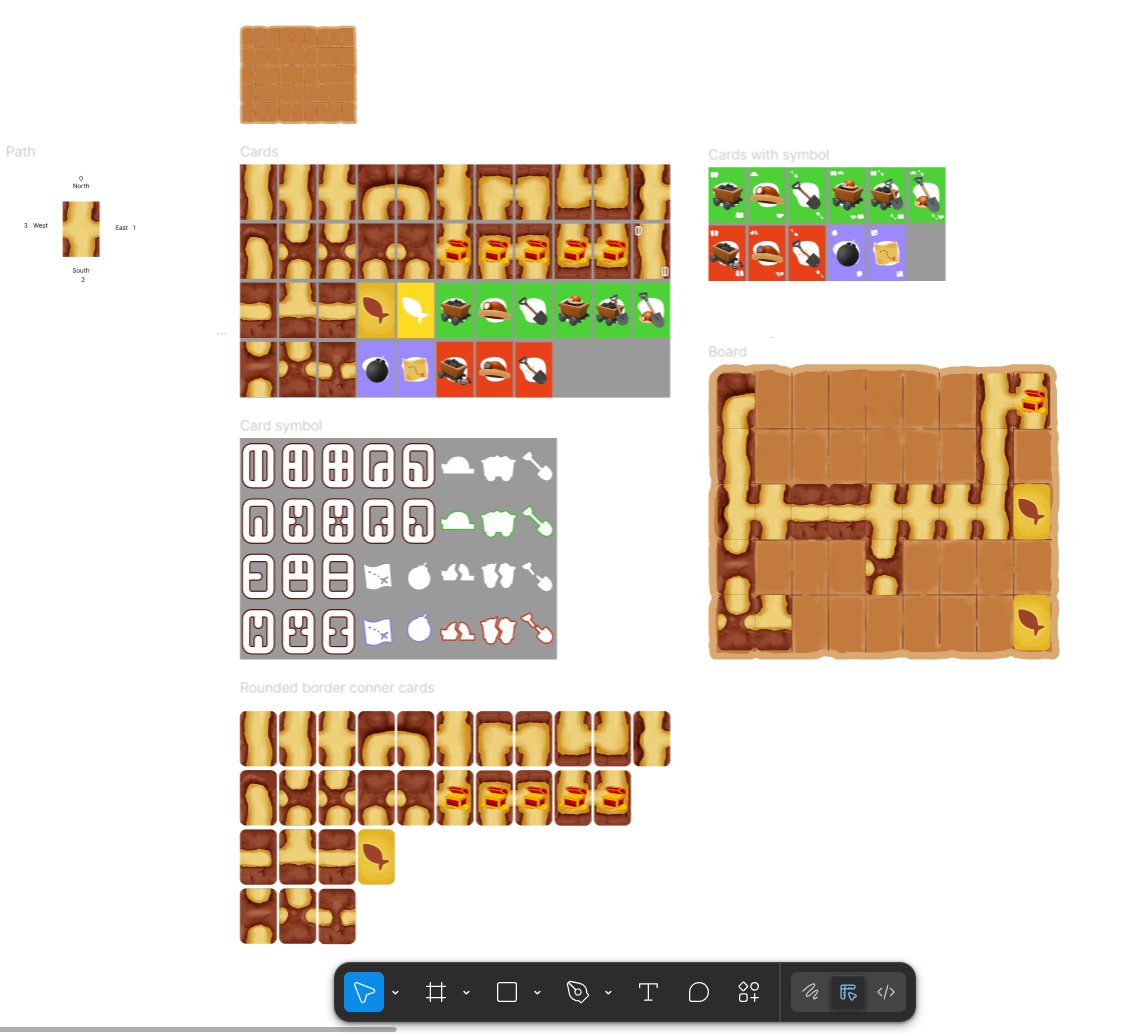
\includegraphics[width=0.75\linewidth]{8. Các thành tựu đạt được/images/CardArts.png}
    \caption{Figma: Bộ thiết kế card}
    \label{fig:placeholder}
\end{figure}

\begin{figure}[H]
    \centering
    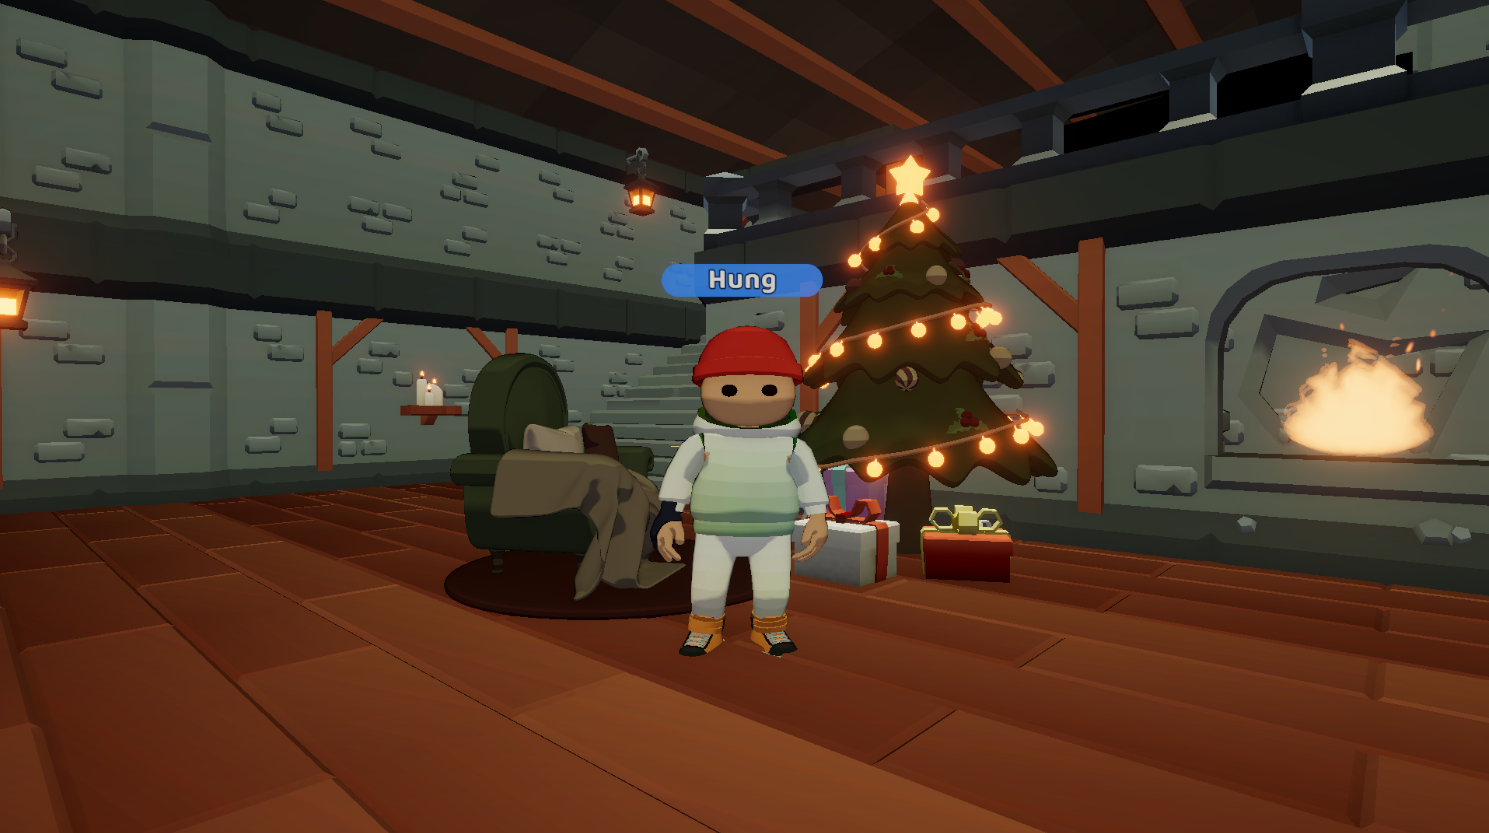
\includegraphics[width=0.75\linewidth]{8. Các thành tựu đạt được/images/character.png}
    \caption{Game Screenshot: Nhân vật khi mới tham gia vào Cabin}
    \label{fig:placeholder}
\end{figure}


\begin{figure}[H]
    \centering
    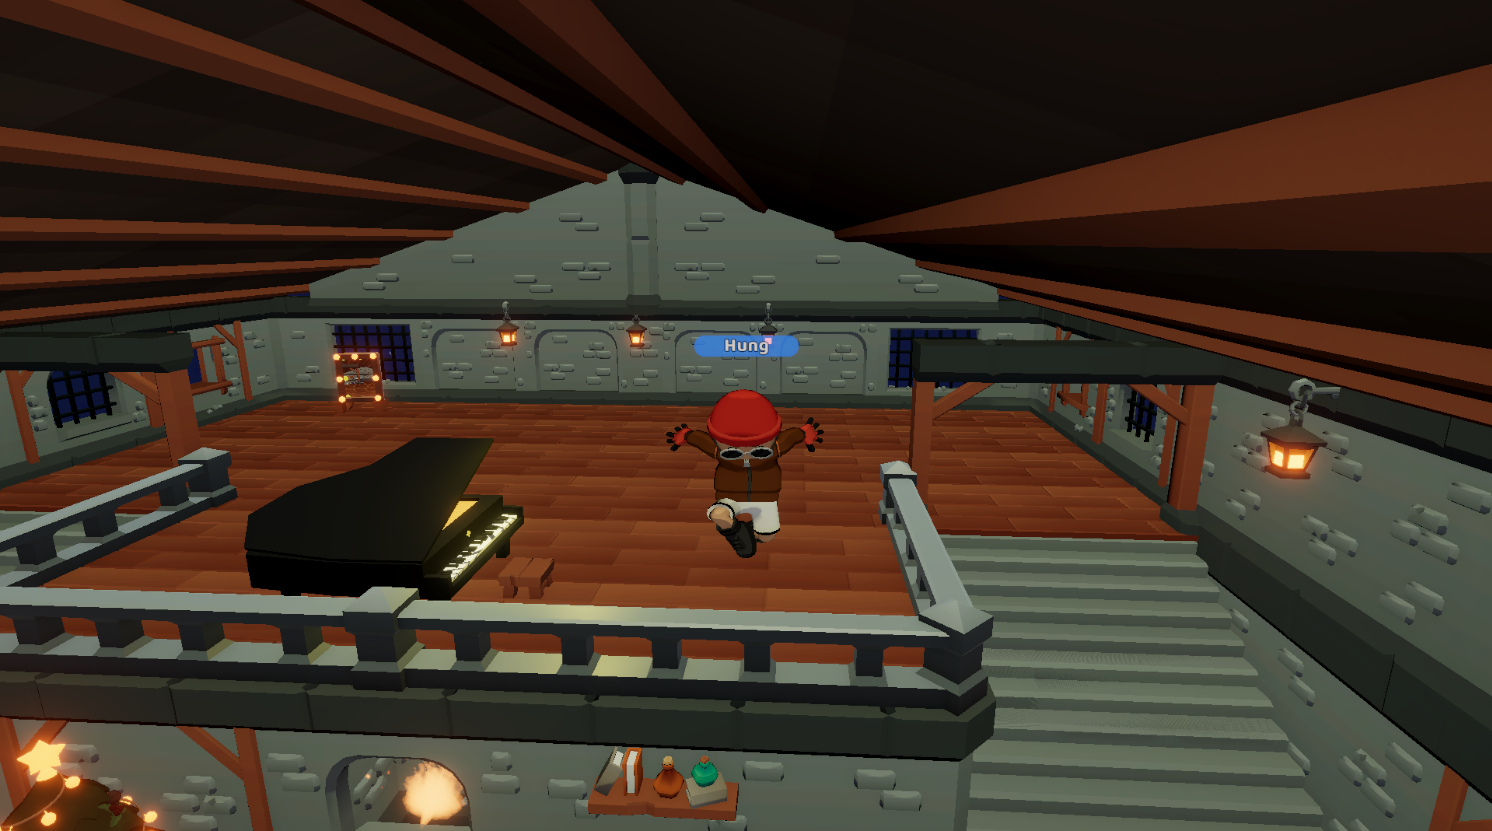
\includegraphics[width=0.75\linewidth]{8. Các thành tựu đạt được/images/jump.png}
    \caption{Game Screenshot: Người chơi nhảy từ gác xuống tầng 1}
    \label{fig:placeholder}
\end{figure}

\begin{figure}[H]
    \centering
    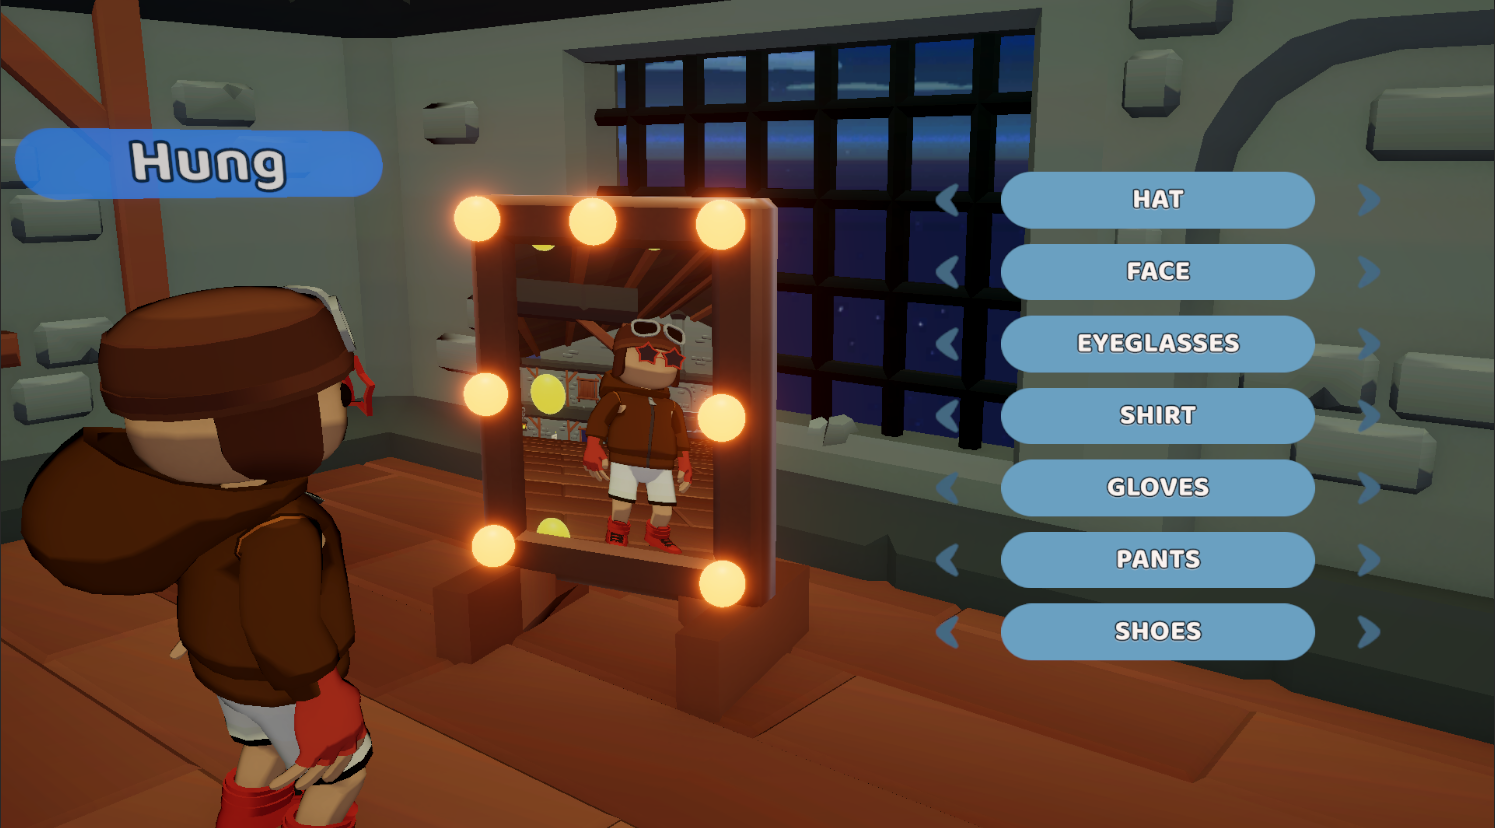
\includegraphics[width=0.75\linewidth]{8. Các thành tựu đạt được/images/mirror.png}
    \caption{Game Screenshot: Người chơi đứng trước gương thay đổi trang phục}
    \label{fig:placeholder}
\end{figure}

\begin{figure}[H]
    \centering
    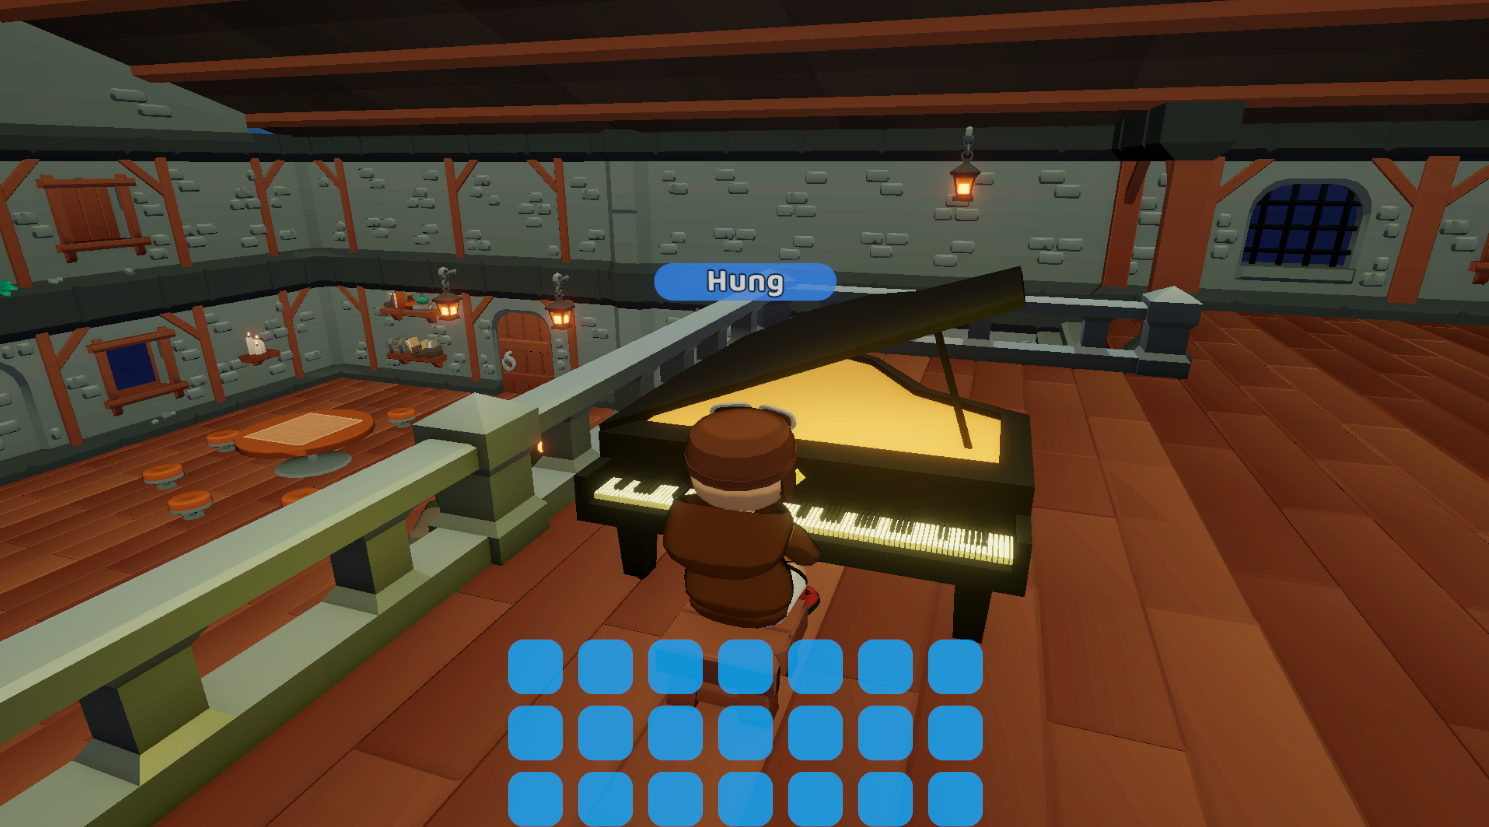
\includegraphics[width=0.75\linewidth]{8. Các thành tựu đạt được/images/piano.png}
    \caption{Game Screenshot: Người chơi chơi đàn piano bằng bàn phím}
    \label{fig:placeholder}
\end{figure}

\begin{figure}[H]
    \centering
    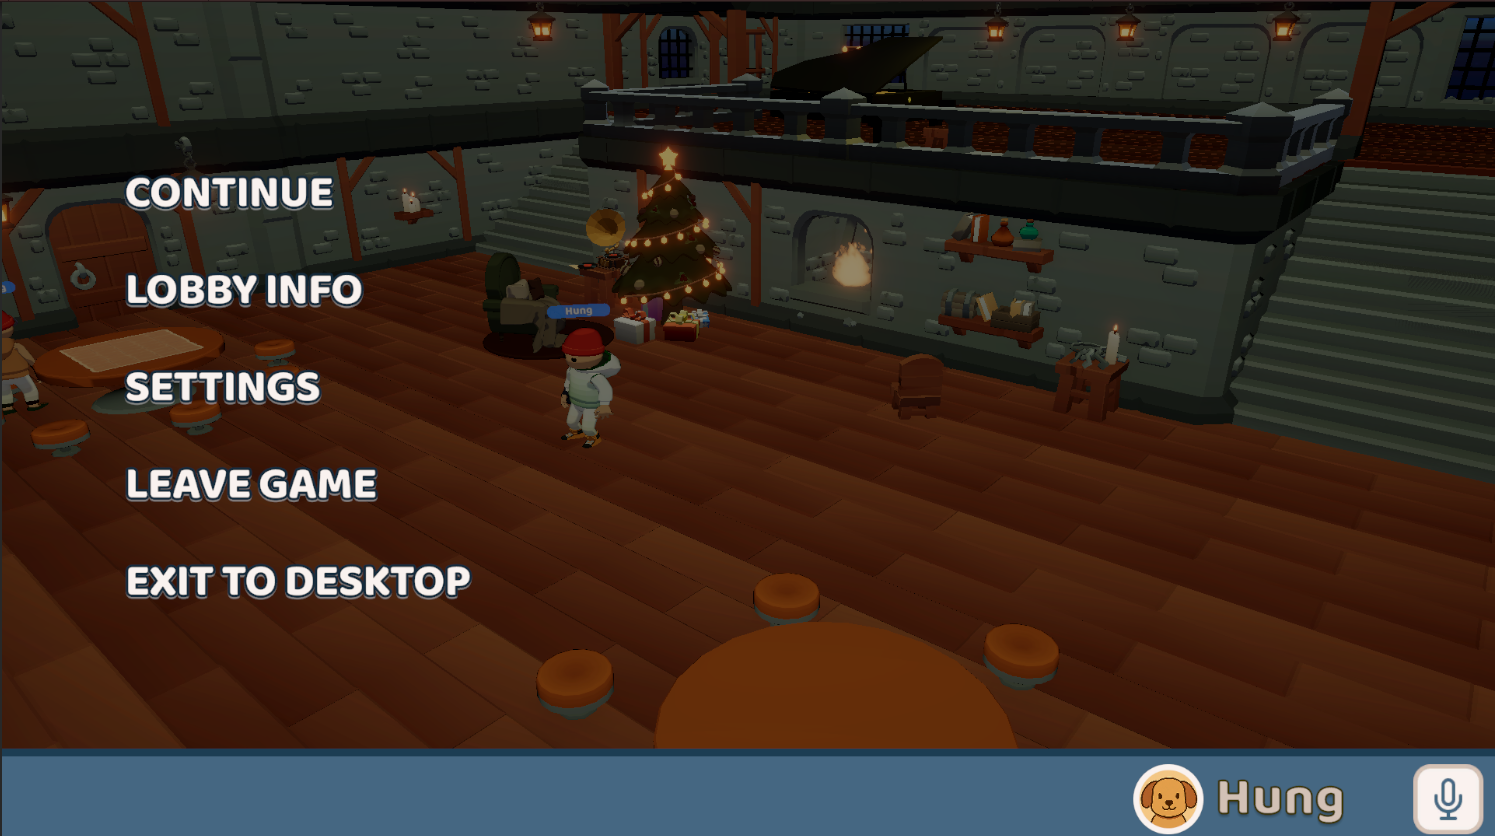
\includegraphics[width=0.75\linewidth]{8. Các thành tựu đạt được/images/ingame-menu.png}
    \caption{Game Screenshot: Menu trong game}
    \label{fig:placeholder}
\end{figure}

\begin{figure}[H]
    \centering
    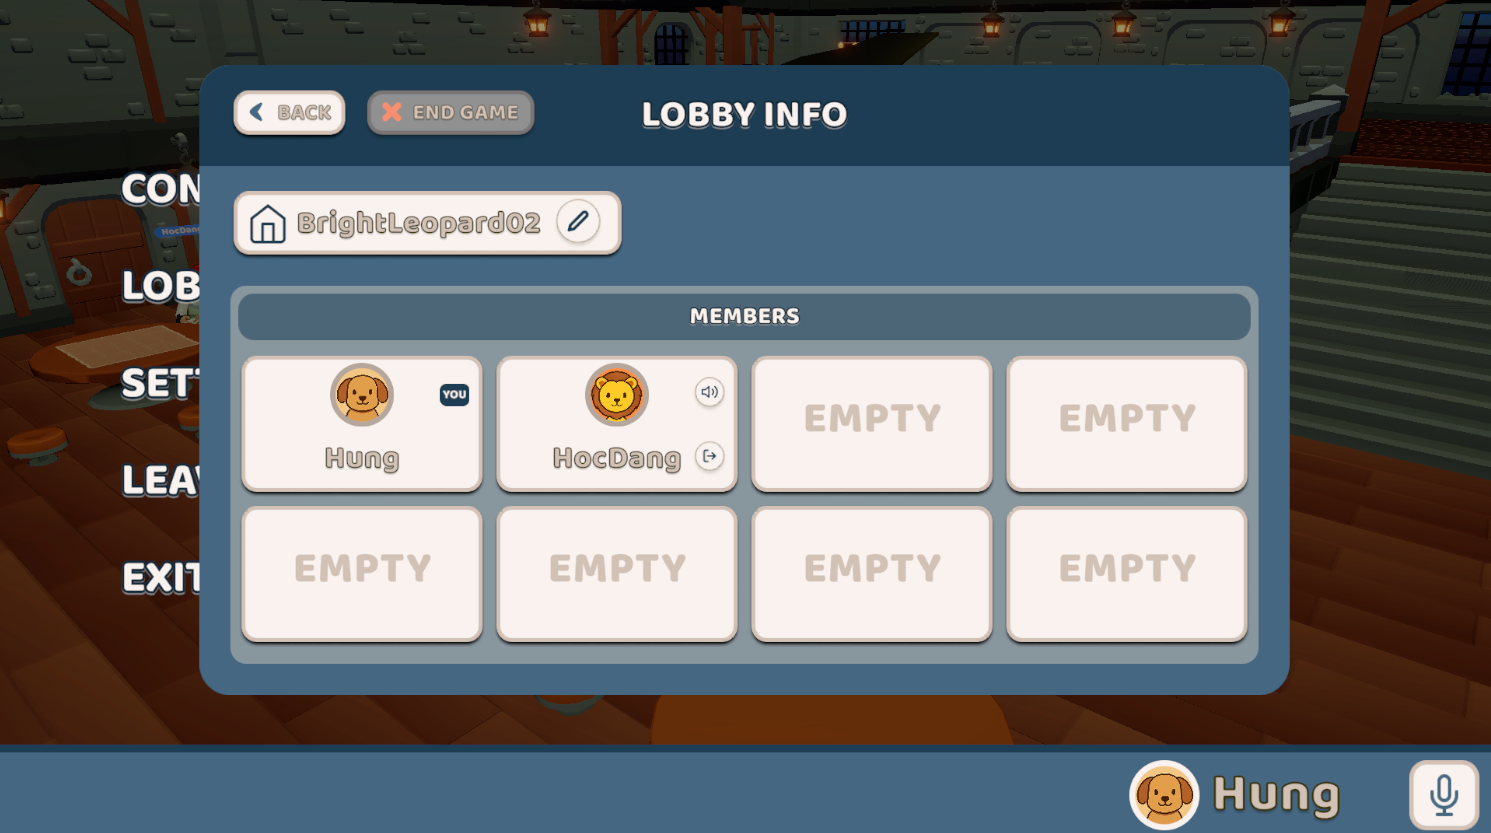
\includegraphics[width=0.75\linewidth]{8. Các thành tựu đạt được/images/lobby-info.png}
    \caption{Game Screenshot: Quản lý lobby, có thể đổi tên phòng, kick người chơi,..}
    \label{fig:placeholder}
\end{figure}

\begin{figure}[H]
    \centering
    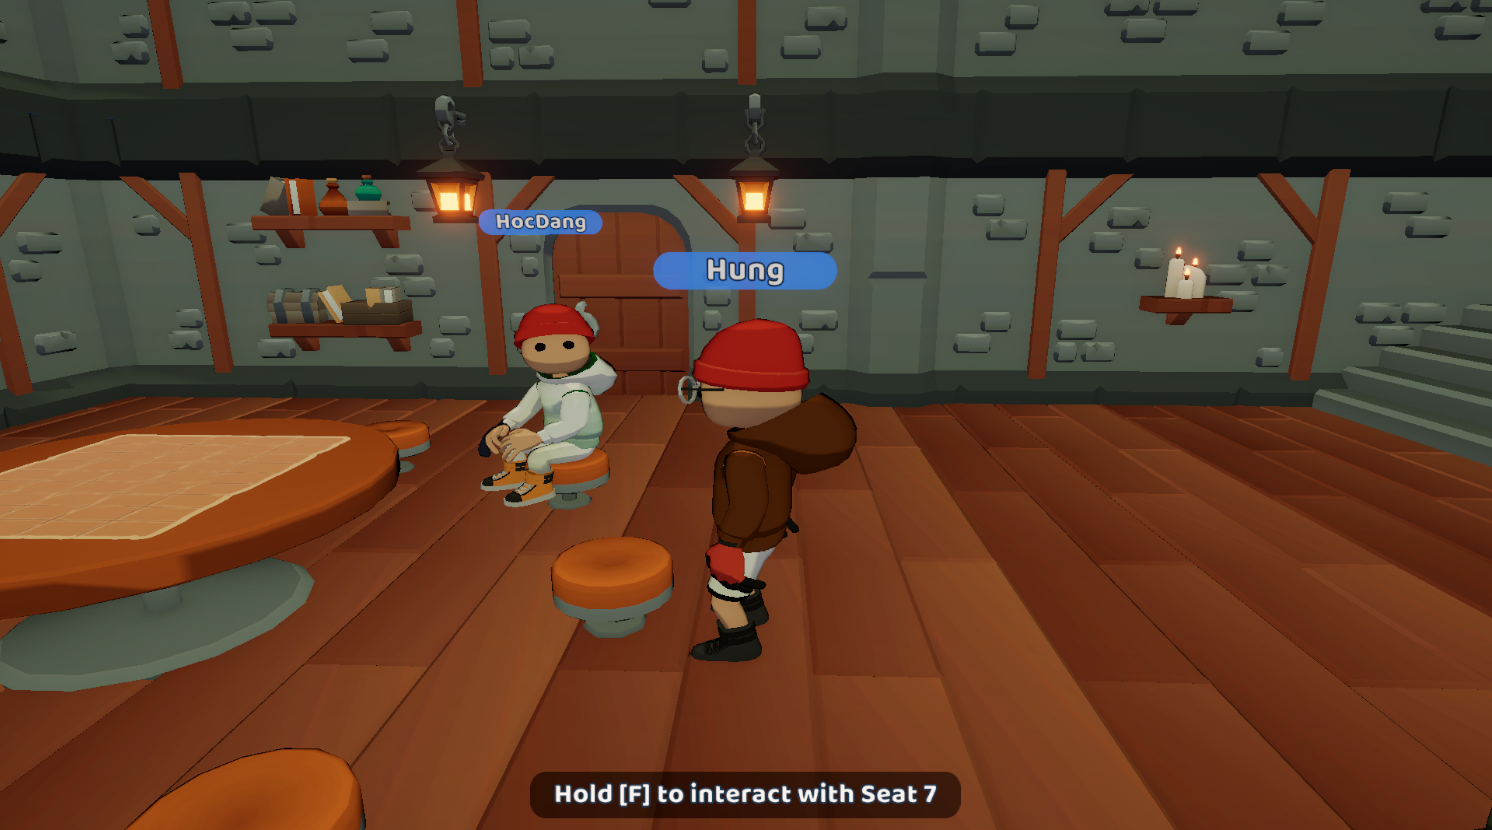
\includegraphics[width=0.75\linewidth]{8. Các thành tựu đạt được/images/interact.png}
    \caption{Game Screenshot: Tương tác với vật thể khi tới gần}
    \label{fig:placeholder}
\end{figure}

\begin{figure}[H]
    \centering
    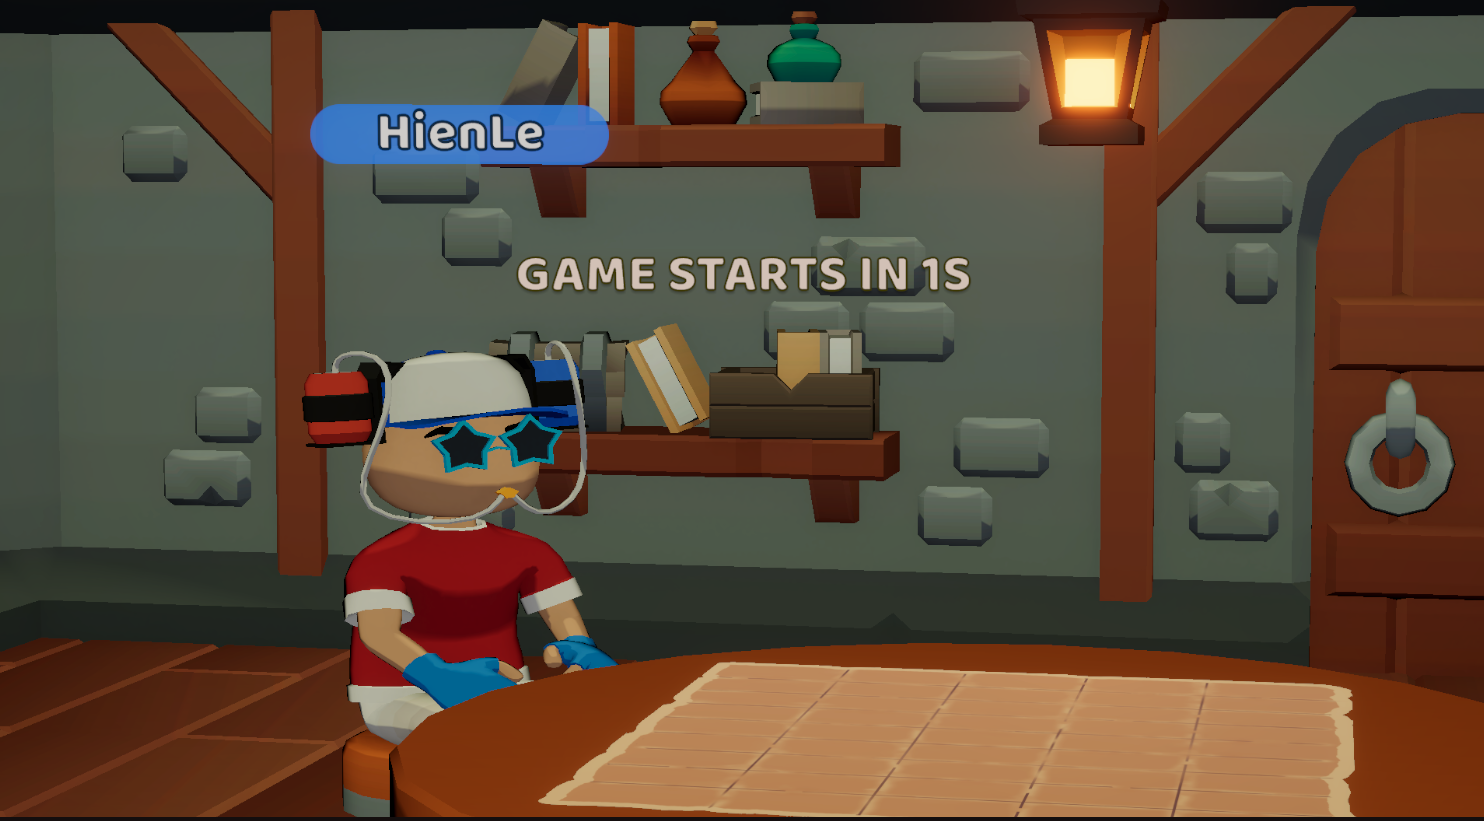
\includegraphics[width=0.75\linewidth]{8. Các thành tựu đạt được/images/start-game.png}
    \caption{Game Screenshot: Người chơi quay đầu nhìn xung quanh}
    \label{fig:placeholder}
\end{figure}


\begin{figure}[H]
    \centering
    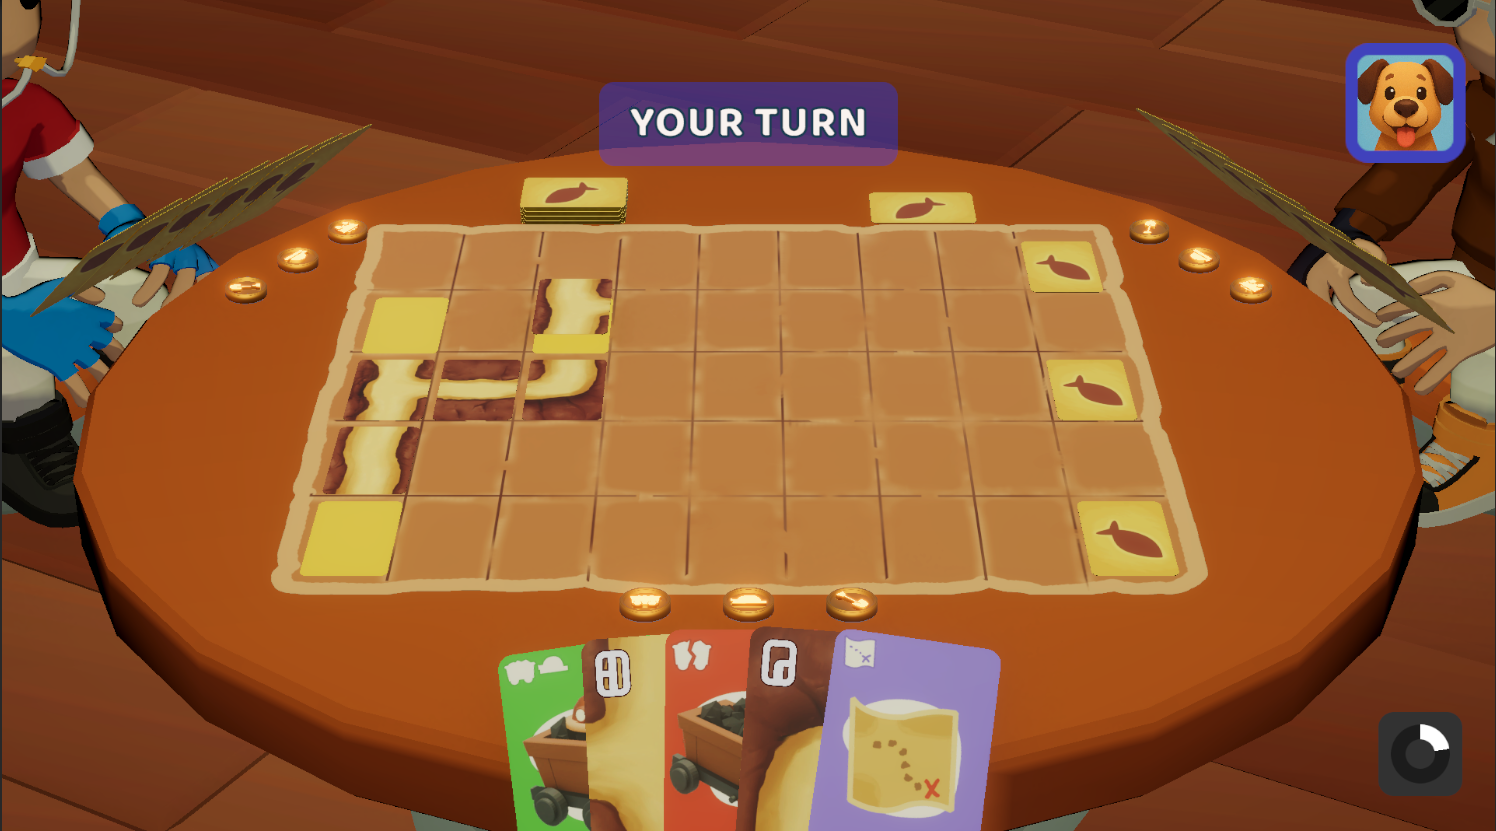
\includegraphics[width=0.75\linewidth]{8. Các thành tựu đạt được/images/playing-card-game.png}
    \caption{Game Screenshot: Khung cảnh của 1 bàn chơi dưới góc nhìn mặc định}
    \label{fig:placeholder}
\end{figure}


\begin{figure}[H]
    \centering
    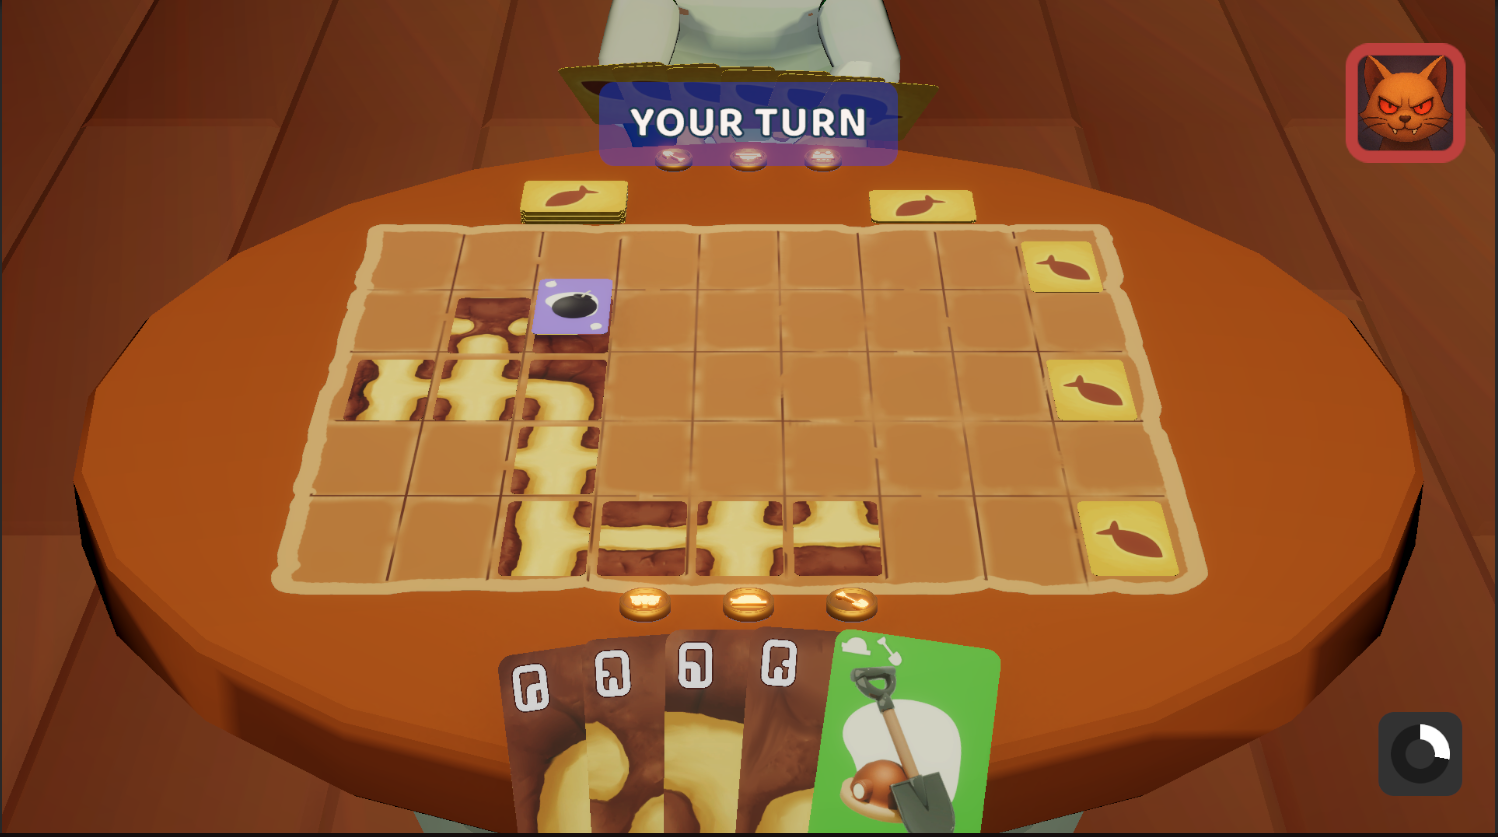
\includegraphics[width=0.75\linewidth]{8. Các thành tựu đạt được/images/bomb.png}
    \caption{Game Screenshot: Sử dụng thể rockfall (bomb) để phá đường}
    \label{fig:placeholder}
\end{figure}


\begin{figure}[H]
    \centering
    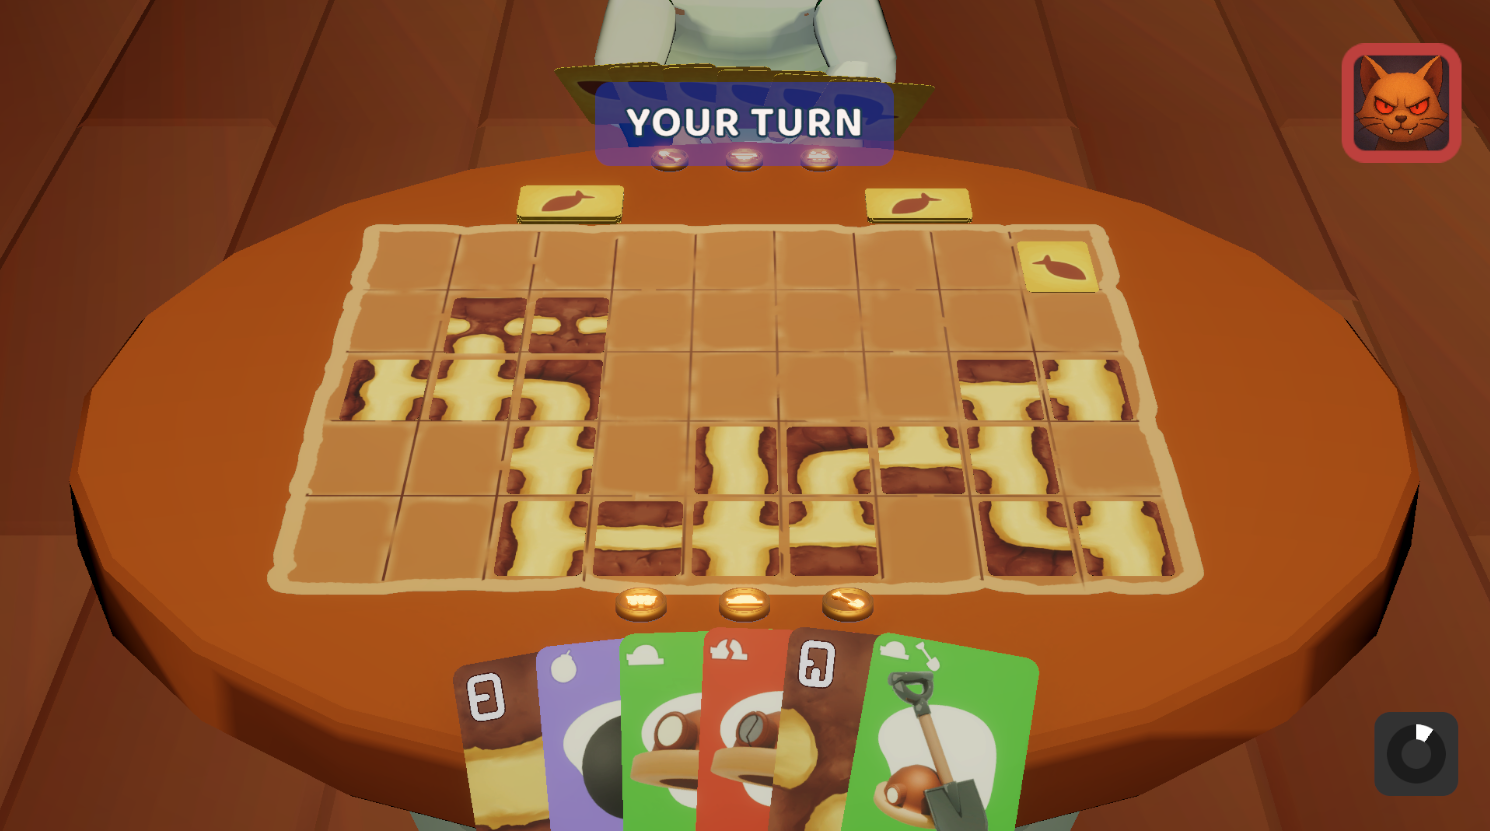
\includegraphics[width=0.75\linewidth]{8. Các thành tựu đạt được/images/empty-goal.png}
    \caption{Game Screenshot: Nối đường tới goal nhưng không chứa vàng}
    \label{fig:placeholder}
\end{figure}

\begin{figure}[H]
    \centering
    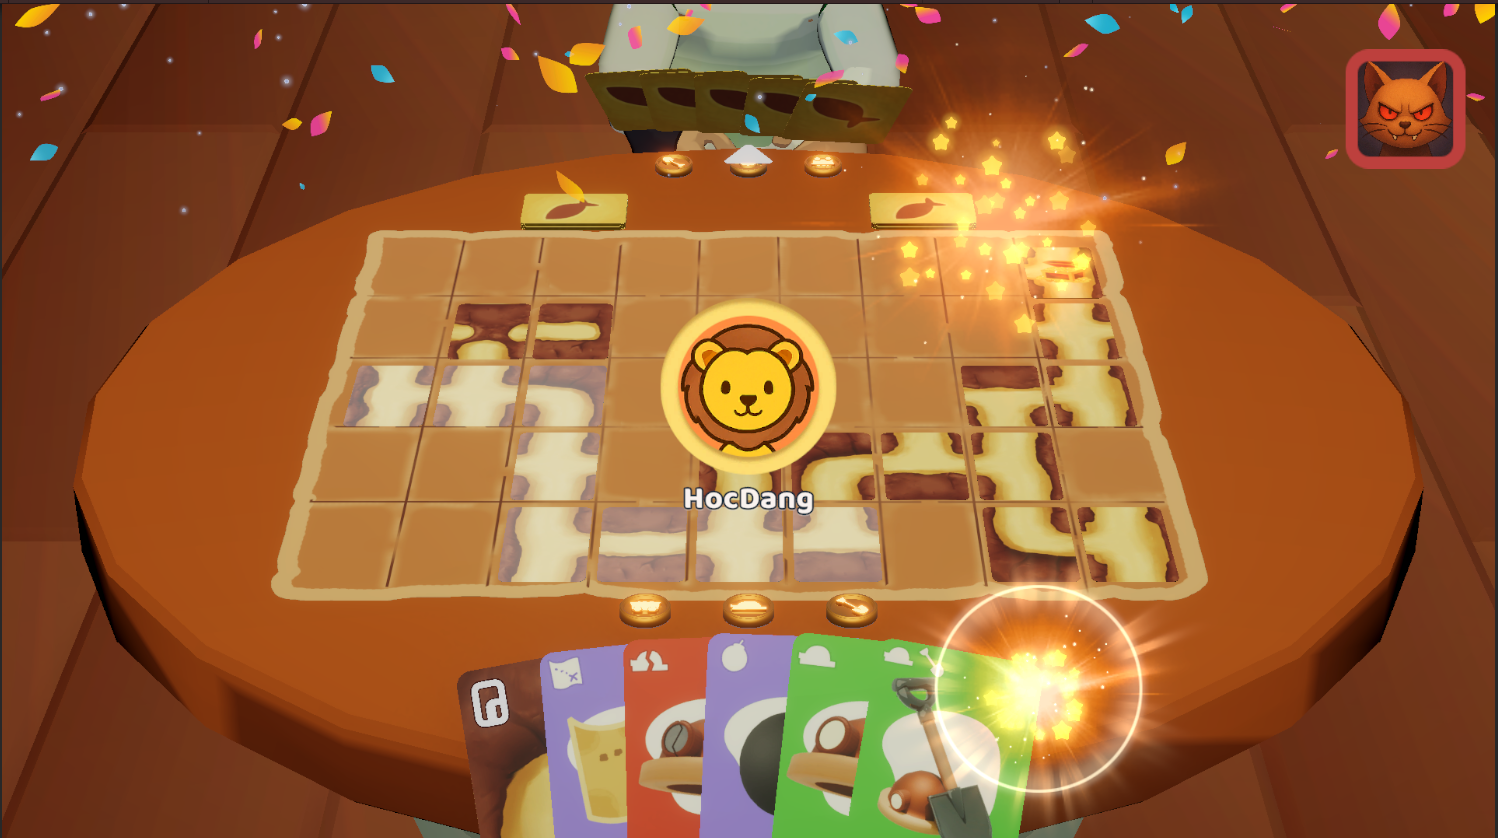
\includegraphics[width=0.75\linewidth]{8. Các thành tựu đạt được/images/end-board-game.png}
    \caption{Game Screenshot: Giao diện thắng/thua khi xong game}
    \label{fig:placeholder}
\end{figure}

% \newpage
\section{Kế hoạch thực hiện giai đoạn tiếp theo}
\subsection{Kế hoạch theo mốc thời gian}

Giai đoạn tiếp theo được triển khai trong vòng 14 tuần, với mục tiêu mở rộng tính năng,
cải thiện trải nghiệm người dùng và nâng cấp kiến trúc hệ thống theo hướng ổn định và
dễ mở rộng hơn. Mỗi tuần được phân rã thành một nhóm nhiệm vụ cụ thể, ưu tiên theo
mức độ quan trọng và sự phụ thuộc lẫn nhau giữa các tính năng. Kế hoạch chi tiết
theo từng mốc thời gian được mô tả trong bảng dưới đây.

% \subsection{Kế hoạch theo mốc thời gian}
\begin{table}[H]
\centering
\begin{tabular}{|c|p{11cm}|}
\hline
\textbf{Tuần} & \textbf{Nội dung công việc chi tiết} \\ \hline


1 & Xây dựng Text Chat: giao diện chat, danh sách người gửi, chống spam, đảm bảo đồng bộ tin nhắn theo thời gian thực. Cơ chế tính điểm cuối trận và hệ thống emoji. \\ \hline

2 & Phát triển hệ thống biểu cảm người chơi (Player's Emotion): tạo thư viện biểu cảm, hoạt ảnh đơn giản, nút chọn nhanh trong giao diện. \\ \hline

3 & Cải thiện tương tác với gameplay: thao tác kéo–thả hợp lý hơn, bổ sung hiệu ứng phản hồi trực quan. \\ \hline

4 & Thêm các map game mới cho người chơi đa dạng lựa chọn. Tích hợp lựa chọn map lên UI trước khi vào game\\ \hline

5 & Tích hợp SFX và VFX: âm thanh thao tác, hiệu ứng mở bài, hiệu ứng hành động, tối ưu hiệu suất tránh gây lag khi kích hoạt liên tục. \\ \hline

6 & Chuyển nền tảng sang mô hình Client–Server (nếu tìm được dịch vụ phù hợp): phân tách logic máy chủ, xử lý đồng bộ trạng thái, kiểm thử tải ở quy mô nhỏ. \\ \hline

7-8 & Thêm board game mới “Liar Bar!”: xây dựng luật chơi cơ bản, UI tối thiểu, chạy thử gameplay loop và kiểm tra lỗi phát sinh. \\ \hline

9 & Tối ưu hiệu suất mạng: giảm độ trễ, cải thiện truyền tải sự kiện, xử lý packet loss, kiểm thử với nhiều người chơi đồng thời. \\ \hline

10 & Nâng cấp và hoàn thiện UI: thiết kế lại các panel chính, thống nhất style, thêm hiệu ứng chuyển cảnh và icon trực quan hơn. \\ \hline

11 & Chuẩn bị bản build phát hành: kiểm thử tính năng, rà soát bug cuối cùng, tối ưu kích thước bản cài. \\ \hline

12 & Deploy và phát hành chính thức lên itch.io: tạo trang mô tả, screenshot, trailer ngắn, thiết lập bản public và kênh cập nhật. \\ \hline

13 & Thu thập phản hồi từ người chơi: khảo sát, ghi nhận lỗi, đánh giá trải nghiệm, phân loại mức độ ưu tiên của vấn đề. \\ \hline

14 & Tổng hợp toàn bộ kết quả, báo cáo tiến độ, đề xuất các cải tiến cho stage tiếp theo và điều chỉnh hướng phát triển lâu dài. \\ \hline

\end{tabular}
\caption{Bảng kế hoạch thực hiện dự án giai đoạn 2}
\end{table}


% \subsection{Kế hoạch phân công nhân sự}

% \begin{table}[h]
% \centering
% \begin{tabular}{|c|p{10cm}|}
% \hline
% \textbf{Thành viên} & \textbf{Nhiệm vụ} \\ \hline
% Người 1 & Phát triển hệ thống mạng, Client–Server, hiệu suất, tích hợp board game mới. \\ \hline
% Người 2 & UI/UX, VFX/SFX, Player Interaction, hệ thống Emotion. \\ \hline
% Người 3 & Map Custom, Text Chat, lobby, publish itch.io, thu thập phản hồi người dùng. \\ \hline
% \end{tabular}
% \end{table}

\subsection{Mục tiêu và kết quả mong đợi}

\begin{itemize}
    \item Hoàn thiện đầy đủ các tính năng cốt lõi của Stage 2: giao tiếp, tương tác, bản đồ tùy chỉnh và UI/UX.
    \item Tối ưu hệ thống mạng để hỗ trợ nhiều người chơi ổn định.
    \item Ra mắt phiên bản công khai trên itch.io để thu hút người dùng đầu tiên.
    \item Thu thập dữ liệu phản hồi từ người chơi nhằm cải thiện chất lượng sản phẩm và định hướng tương lai.
\end{itemize}


\newpage
% \section{Kết luận và hướng phát triển}
\subsection{Tóm tắt kết quả đạt được}
\subsection{Hạn chế của đề tài}
\subsection{Hướng phát triển tương lai}
%%%%%%%%%%%%%%%%%%%%%%%%%%%%%%%%%%%%%%%%%%%%

\newpage
\section{Tài liệu tham khảo}
\begin{thebibliography}{9}

\bibitem{saboteur2024}
AMIGO Spiel + Freizeit GmbH.
\textit{Saboteur: Offizielle Spielanleitung}.
Regelbuch (Artikel-Nr. 18750), AMIGO Spiel, 2024.
Truy cập ngày 13 tháng 12 năm 2025.
Available at: \url{https://www.amigo.games/wp-content/uploads/2024/08/18750-ur.pdf}

\bibitem{madhav2013}
Sanjay Madhav.
\textit{Game Programming Algorithms and Techniques: A Platform-Agnostic Approach}.
Addison-Wesley, 2013.
ISBN: 9780321940155.

\bibitem{unity_patterns}
Unity Technologies.
\textit{Level Up Your Code with Game Programming Patterns}.
E-book, Unity Technologies, 2022.
Truy cập ngày 13 tháng 12 năm 2025.
Available at: \url{https://unity.com/resources/level-up-your-code-with-game-programming-patterns}

\bibitem{unity_scriptableobjects}
Unity Technologies.
\textit{Create Modular Game Architecture in Unity with ScriptableObjects}.
E-book, Unity Technologies, 2023.
Truy cập ngày 13 tháng 12 năm 2025.
Available at: \url{https://unity.com/resources/create-modular-game-architecture-with-scriptable-objects-ebook}

\bibitem{hipple2017}
Ryan Hipple.
\textit{Unite Austin 2017 - Game Architecture with Scriptable Objects}.
Video presentation at Unite Austin 2017, Unity Technologies, 20 tháng 11 năm 2017.
Truy cập ngày 13 tháng 12 năm 2025.
Available at: \url{https://www.youtube.com/watch?v=raQ3iHhE_Kk}

\bibitem{vivox2025}
Unity Technologies.
\textit{Vivox Unity SDK documentation}.
Unity Gaming Services Documentation, phiên bản 16.
Truy cập ngày 13 tháng 12 năm 2025.
Available at: \url{https://docs.unity.com/ugs/en-us/manual/vivox-unity/manual/Unity/Unity}

\bibitem{netcode2025}
Unity Technologies.
\textit{Netcode for GameObjects Manual (Version 2.7.0)}.
Unity Package Documentation.
Truy cập ngày 13 tháng 12 năm 2025.
Available at: \url{https://docs.unity3d.com/Packages/com.unity.netcode.gameobjects@2.7/manual/index.html}

\bibitem{unitymultiplayer2025}
Unity Technologies.
\textit{Multiplayer - Unity Manual (Unity 6.2)}.
Unity Documentation.
Truy cập ngày 13 tháng 12 năm 2025.
Available at: \url{https://docs.unity3d.com/6000.2/Documentation/Manual/multiplayer.html}

\bibitem{appwill2025}
AppWill Inc.
\textit{Multiplayer in Unity: Best Networking Solutions 2025 | Ultimate Guide}.
Blog post, ngày 24 tháng 6 năm 2025.
Truy cập ngày 13 tháng 12 năm 2025.
Available at: \url{https://appwill.co/multiplayer-in-unity-best-networking-solutions-2025/}
\end{thebibliography}
\end{document}

